\documentclass[12pt]{ociamthesis}  % default square logo 
%\documentclass[12pt,beltcrest]{ociamthesis} % use old belt crest logo
%\documentclass[12pt,shieldcrest]{ociamthesis} % use older shield crest logo

%load any additional packages
\usepackage{amssymb,amsthm, amsmath}
\usepackage{graphicx}
\usepackage{setspace}
\usepackage{epsfig,epstopdf}
\usepackage{subcaption}
\usepackage{caption}
\usepackage{multirow}
\usepackage{makecell}
%\usepackage{pbox}
\usepackage{algorithm,algpseudocode}
\usepackage{url}
\usepackage[normalem]{ulem}
\usepackage{multirow,booktabs}

\usepackage{todonotes}
\usepackage{xcolor}



\graphicspath{ {./Charts/}}
\epstopdfsetup{outdir=./Charts/}

\theoremstyle{definition}
\newtheorem{example}{Example}[section]
\newtheorem{theorem}{Theorem}[section] % reset theorem numbering for each chapter
\newtheorem{definition}{Definition}[section]
\newtheorem{query}{Query}[section]
\newtheorem{lemma}[theorem]{Lemma}


\DeclareMathOperator*{\argmin}{argmin}
\DeclareMathOperator*{\argmax}{argmax}
\DeclareMathOperator*{\triu}{triu}
\DeclareMathOperator*{\range}{range}
\newcommand*{\argminl}{\argmin\limits}
\newcommand*{\argmaxl}{\argmax\limits}
\renewcommand{\algorithmicrequire}{\textbf{Input:}} 
\newcommand{\revised}[1]{{\color{red}{#1}}}
\newcommand{\doubted}[1]{{\color{blue}{#1}}}
\newcommand{\eat}[1]{ }
\newcommand{\original}[1]{\sout{#1}}


\includeonly{chapter1/chapter1, chapter2/chapter2}

%input macros (i.e. write your own macros file called mymacros.tex 
%and uncomment the next line)
%\include{mymacros}

\title{Codimension-Two\\[1ex]     %your thesis title,
        Free Boundary Problems}   %note \\[1ex] is a line break in the title

\author{Keith Gillow}             %your name
\college{National University of Singapore}  %your college

%\renewcommand{\submittedtext}{change the default text here if needed}
\degree{Doctor of Philosophy}     %the degree
\degreedate{Dec 2016}         %the degree date

%end the preamble and start the document
\begin{document}

%this baselineskip gives sufficient line spacing for an examiner to easily
%markup the thesis with comments
\baselineskip=18pt plus1pt
\doublespacing

%set the number of sectioning levels that get number and appear in the contents
\setcounter{secnumdepth}{3}
\setcounter{tocdepth}{3}

%\maketitle                  % create a title page from the preamble info
%\begin{dedication}
This thesis is dedicated to\\
 someone\\
for some special reason\\
\end{dedication}        % include a dedication.tex file
%\begin{acknowledgements}
I could not have completed this thesis without the help and support of many people.
It is my great pleasure to take this opportunity to thank all of them.
%
%Hereby, I would like to express my deepest gratitude to many people without whom this
%thesis would not have been completed.

First and foremost, I would like to express my utmost appreciation to 
my supervisor, Prof.~Kian-Lee Tan. Throughout my doctoral study, I have
received innumerable guidance and inspirations from him. His knowledgeable
insights play an important role in completing this thesis. As
a supervisor, he not only imparts me the rigorous research attitude
but also exemplifies a strong personality with
humility and gentleness. 
I would also like to mention his provision of the research assistant position which
sponsors me for the fifth year study. It is my privilege to be his student.

Second, I would like to deeply thank Prof.~Anthony K.~H.~Tung, Prof.~Shui-cheng Yan 
and Prof.~Roger Zimmermann for constituting my thesis advisory committee. 
I appreciate their efforts and time in monitoring and guiding my research with
inspiring comments. 


Third, I would like to especially thank Prof.~Zhengkui Wang and Prof.~Dong-xiang Zhang.
Prof.~Wang guided me on my first work which was a good starting point.
Prof.~Zhang has closely collaborated with me during my doctoral study. They
both generously shared me with the valuable knowledge on technical development 
and critical writing, which strengthened 
the technical quality and
literature presentation of my thesis.
I would not forget the assistance from my collaborators: Professor Chee-Yong Chan,
Dr.~Yuchen Li and Dr.~Huayu Wu. They have spent a lot of their precious time to greatly improve
our papers. It is fruitful to work with them.

Furthermore, I would like to thank NUS Graduate School of Integrative of Science and
Engineering (NGS) for offering me the scholarship.

Next, I feel lucky to have many friends during my academic
pursuit. They are Prof.~Zhifeng Bao, Dr.~Qian Xiao, Dr.~Htoo Htet Aung,
Dr.Long Guo, Dr.~Yong Zeng, Dr.~Zong Zeng, Dr.~Jingbo Zhou, Dr.~Yuxin Zheng, Yingjun Wu, Wentian Guo,
Yanhao Wang, Mo Sha, Qing Liu, Meiying Li, Qi Guo and Jiangwei Zhang. I would also 
like to thank my friends in Database Basketball Group %and Database Foosball Group
as we have shared wonderful memories.

Last but not least, the most special gratitude is reserved for my beloved family: my parents Xiaoquan Fan and Jiangrong Qi,
my parents-in-law Guangchen Cui and Yumei Zhang, and my dearest wife Sophia Xiang Cui.
Their unconditional support, persistent accompaniment, and consistent love
sustain me through the otherwise grueling Ph.D.~study.

%which has sustained me through the otherwise grueling period of my
%doctoral study
%
%
%through the otherwise grueling Ph.D.~study.

%My most appreciation is for my dearest wife Sophia Cui, 
%who provides me persistent accompany and love through the otherwise grueling Ph.D.~period.
%First and foremost, I would like to express my most profound gratitude to
%my supervisor, Prof. Beng Chin Ooi. Without him, I would not be able to
%complete my PhD program successfully. I was not from top university and
%did not come with very strong foundation and programming skills when I was
%admitted to the PhD program. I sincerely thank Prof. Ooi for his patience,
%guidance and support that helped me get through tough times and shape my
%research skills. I also thank him for offering me the opportunities to visit
%research labs and collaborate with accomplished researchers. It has been my
%great honor to be his student
%
%I would like to express my heartfelt gratitude and appreciation for his invaluable guidance
%and inspiration in this research, his moral support and encouragement during the duration
%of my Ph.D study. It is a privilege to work under him, and he has set a good example to
%me in many different ways. His insights and knowledge in this area play an important
%role in completing this thesis. As a supervisor, he shows me not only how to be a good
%researcher with rigorous research attitude, but also how to build a good personality with
%humility and gentleness. All that I have learned from him will be of great influence for
%my research and my entire life.
% 
%
%This thesis would not have been completed without the support of many people. I
%would like to reserve this section to express my gratitude to all of them.
%
%
%I would hereby express my gratitude to the people that have been ... without whom this thesis cannot be accomplished. 
%
%My utmost gratitude goes to my main supervisor, Prof. Kian-Lee Tan, for his constant and painstaking efforts in inspiring me to explore
%beyond the boundary of my research topic during my candidature. It has been a
%remarkable experience to conduct research under Professor Tan's guidance. During
%the time, he has shared much of his experience, knowledge and wisdom to me, which
%will surely benefit every aspect of my life. Regarding to research, he has always taught
%me to zoom in and zoom out when solving a particular problem, and this insight had
%deep impact on my research. Prof. Tan also provided me with many opportunities to
%stay in touch and collaborate with both local and global prestigious researchers which
%were invaluable experiences and broadened my horizon. I would also like to sincerely
%thank my TAC members, Prof. Anthony Tung, Prof Roger Zimmermann and Prof. Shuicheng Yan for the valuable guidance and support
%during my Ph.D. study. 
%
%I have been fortunate to work with these brilliant people
%who are generous with their time and friendship. My special thanks also go to my dear fellow colleagues. Without them, I would not have had such a meaningful Ph.D. life.
%Thank them for bringing me so many fond memories. I am also grateful to all the
%other staffs, fellow colleagues and friends in the Robotics Research Lab, the Social
%Robotics Lab and Advanced Robotics Center for their companionship, generous help
%and collaborations.
%
%I am also very grateful to National University of Singapore for providing me with a great opportunity and financial support to pursue my Ph.D. degree.
%
%Last but not least, I wish to thank my family, especially my parents and parents in-law, providing me the freedom to pursue my dream. My preserved thanks always goes to my wife Sophia, who consistently stands by me and give priceless support.
\end{acknowledgements}   % include an acknowledgements.tex file
%\begin{abstract}
With the increasing variety and volume of the data 
produced by today's applications, the adoption of effective 
analytics becomes remarkably demanding. Window functions,
being an important part of SQL family, have proven numerous successes in
relational analytics. A window function 
assigns each tuple a set of related tuples, on which analytics can be applied.
However, the window function defines the related tuples based on sorting which
limits its usage in the domains where sorting may not be meaningful.
In this thesis, we generalize the concept the window function to 
\emph{neighborhood analytics} which eliminates the stringent sorting requirement.
We propose three domain-specific queries tailored for emerging applications 
on the basis of two simple neighborhood functions.
Then, we study how to process these queries efficiently given today's data scale.

In particular, we first propose the \emph{Graph Window Query} (GWQ) in the graph domain. 
GWQ computes aggregation for each vertex on its graph window. We formally define
two instances of such graph windows: $k$-hop window and topological window. Then,
we develop the Dense Block Index (DBIndex) and Inheritance Index (I-Index) to
facilitate efficient processing of both queries. These indexes effectively compress
the windows of each vertex and reuse the shared components during query processing, 
which achieve both space and query efficiency. 

%We conduct extensive experimental evaluations
%over both large-scale real and synthetic datasets. The results verifies the 
%efficiency and scalability of our proposed indexes.


Second, we propose the $k$-Sketch query on the sequence data to summarize a subject's history.
$k$-Sketch query utilizes the novel \emph{ranked-streak} 
which is formed by a nested neighborhood function. Specifically, a streak is first constructed
by grouping temporally nearby events. Subsequently, streaks with the same length are 
compared to generate their ranks. 
A $k$-Sketch query then selects $k$ ranked-streaks which best summarize
a subject's history.
We study the $k$-Sketch query processing in both offline and online scenarios. 
In particular, we design two nontrivial streak-level pruning techniques and a $(1-1/e)$-approximate algorithm to achieve efficient processing in offline. Then we design a $1/8$-approximate algorithm for the online sketch maintenance. 
%Our comprehensive experiments demonstrated the efficiency of our solutions and a human study confirms the effectiveness of the $k$-Sketch query.

% two efficient pruning methods to quickly
%compute all \emph{ranked-streak}, and then we design a $1-1/e$ approximate solution to 
%find the $k$-Sketch. In the online scenario, we propose an efficient pruning method
%to avoid examine all the ranked-streak. We further design a $1/8$-approximate solution
%to find the online $k$-Sketch. 
%We conduct efficiency study on three real datasets. Our 
%solution achieves hundred times boost as compared to baselines. Besides, the effectiveness
%of our solution is also endorsed by the anonymous users from Amazon Mechanical Turk.

Third, we propose the General Co-Movement Pattern (GCMP) query for trajectory databases. A GCMP
is defined as the temporal invariant portion of an object's spatial neighborhood. Our GCMP
is versatile to express other moving patterns defined in the literature. Meanwhile, GCMP
is also able to eliminate the so-called loose-connection anomaly which has not been addressed before.
We design two parallel frameworks for supporting scalable GCMP detection. First, we propose
a baseline method named \emph{Temporal Replication and Parallel Mining} (TRPM) 
which partitions trajectories via replication of object locations and mines
GCMPs from each partition in parallel.
Then, we design an advanced method named \emph{Star Partition and ApRiori Enumerator} (SPARE)
to resolve the limitations of TRPM. We adopt three novel techniques in SPARE to achieve load balance 
while minimizing data replications. To the best of our knowledge, this is the first work which
detects co-moving patterns from trajectories with hundreds of millions of data points.

\end{abstract}          % include the abstract

%\begin{romanpages}          % start roman page numbering
%\tableofcontents            % generate and include a table of contents
%\listoffigures              % generate and include a list of figures
%\end{romanpages}            % end roman page numbering

%now include the files of latex for each of the chapters etc
\chapter{Introduction}
With the maturity of database technologies, nowadays
applications collect data in all domains at an
unprecedented scale. For example, billions of 
social network users and their activities are collected in the form
of \emph{graphs}; Thousand sensor reports are collected per second
in the form of \emph{time series}; Hundreds of millions of temporal-locations
are collected as \emph{trajectories}, to name just a few. Flooded by the
tremendous amount of data, it is emerging to 
provide useful and efficient analytics for various data domains.
Traditional SQL analytics which comprises 
of operations (such as, partition, sorting and aggregation) in the relational domain
become limited in non-structured domains.
In SQL context, interesting analytics such as graph traversal and pattern detection
often involve complex joins which are very hard to optimize 
without domain knowledge.
In this thesis, we explore the neighborhood data analytic, which
in SQL is expressed by the window function,
on different domains and demonstrate how to efficiently deploy
neighborhood analytic to gain useful insights.

\section{Neighborhood Analytics}
Followed by its self-descriptive name, neighborhood analytics aims to provide
summaries of each object over its vicinity. In contrast to aggregating the entire collection of data as a whole, neighborhood
analytic provides a personalized view for each object from its own perspective. Neighborhood
data analytics originates from the window function defined in SQL which is
illustrated in Figure~\ref{fig:window}.

\begin{figure}[h]
\centering
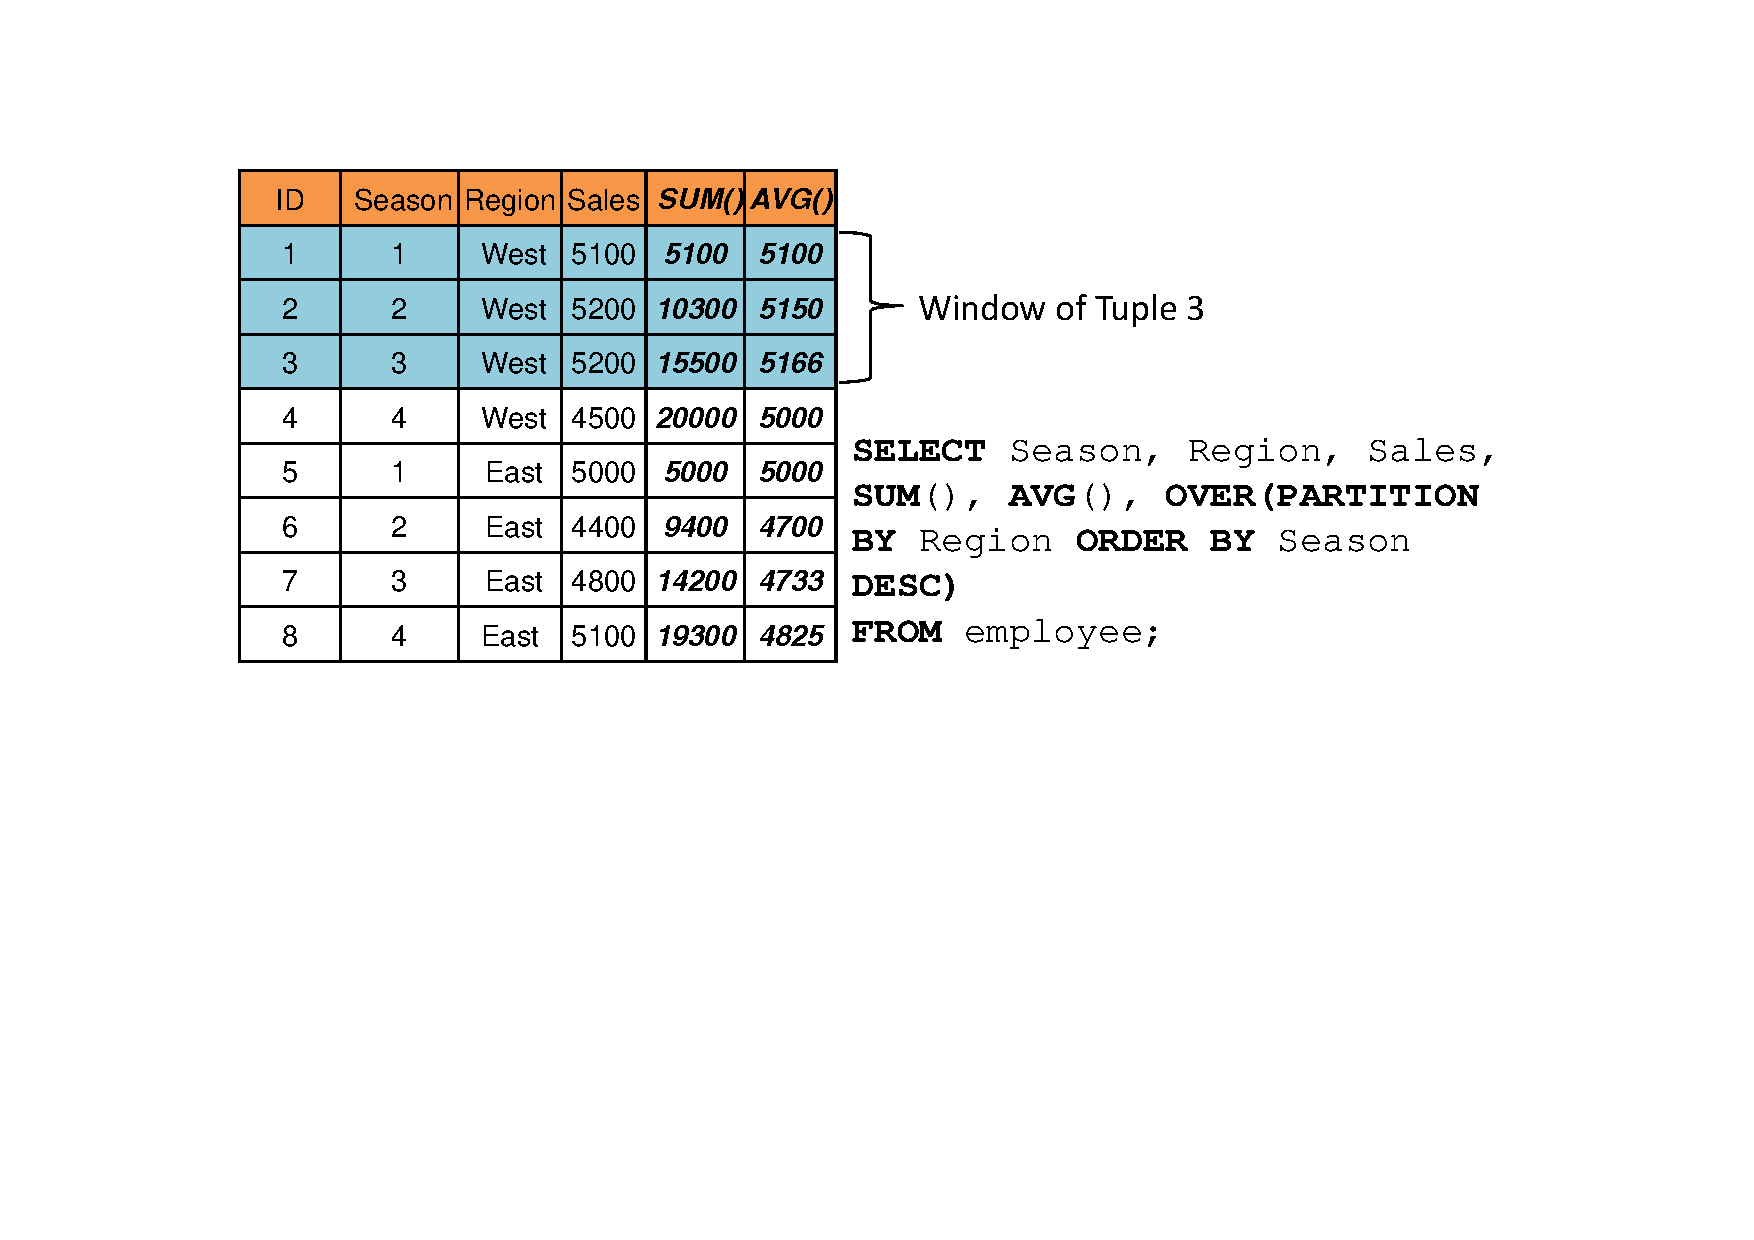
\includegraphics[width=0.8\linewidth]{window_example.pdf}
\caption{A SQL window function computing running sum and average of
sales. The window of tuple 3 is highlighted.} 
\label{fig:window}
\end{figure}

As shown in the figure, the sales report contains six columns: ``ID'',
``Season'', ``Region'' and ``Sales'' are the \emph{facts}, ``$\mathtt{sum()}$'' and ``$\mathtt{avg()}$''
are the \emph{analytics} representing the running sum and average. A window function
is represented by the $\mathtt{over}$ keyword. In this context, the window of a tuple $o_i$
contains other another tuple $o_j$ if $o_i$ and $o_j$ are in the same ``region'' and the``season'' of $o_j$ is
prior to the season of $o_i$. The window of tuple-$3$ is highlighted.
Apart from this example, there are also many other 
usages of the window functions in the relational context~\cite{cao2012optimization}. 
Being aware of the success of the window functions, 
SQL~11~\cite{zemke2012s} standard incorporates ``$\mathtt{LEAD}$'' and ``$\mathtt{LAG}$'' 
keywords to offer fine-grained specifications on a tuple's window.

Despite the usefulness, there are few works reporting
the usage of window functions in data domains such as graphs, sequence data and trajectories.
This may due to the
requirement of \emph{sorting} in the window functions. For example,
in Figure~\ref{fig:window},
objects need to be sorted according to ``Season'', and then the window of
each objects is implicitly formed based on the sorted order. However, 
in other data domains, sorting may be ambiguous and even undefined.

To broaden the usages of the window functions in other data domains, we propose the \emph{neighborhood
analytics} in a more general sense. Given a set of objects 
(such as tuples in relational tables, vertexes in graphs, moving objects in trajectories),
the neighborhood analytics is a composite function
$(\mathcal{F} \circ \mathcal{N})$ applied on every object. Here, $\mathcal{N}$
is the \emph{neighborhood function}, which contains the related objects (i.e., vicinity) of an object;
$\mathcal{F}$ is the \emph{analytic function}, which could be aggregation, ranking,
pattern matching, etc.
Apparently, the SQL window function is a special case of the
neighborhood analytics. For example, the window function in Figure~\ref{fig:window} 
can be represented as $\mathcal{N}(o_i)=\{o_j | o_i.season > o_j.season \wedge o_i.region = o_j.region\}$
and $\mathcal{F} = \mathtt{avg}$.
By relaxing the sorting constraint, neighborhood analytics gains an enriched 
semantic and can be applied on many other data domains.

%Since the \emph{sorting} requirement is relaxed, our neighborhood analytics is able to
%enrich the semantic of relational window notations 
%and can be applied on many other domains.
\section{Thesis Scope}
In this thesis, we explore the neighborhood analytics in emerging applications
from three prevalent data domains, namely \textbf{attributed graph},
\textbf{sequence data} and \textbf{trajectory}. 
To provide useful analytics, we define the following
two intuitive instances of the neighborhood function:
%Since the neighborhood analytics could be very broad,
%this thesis only focus on the following 
%two intuitive neighborhood functions:

\textbf{Distance Neighborhood}: the neighborhood is defined based on numeric distance, that is $\mathcal{N}(o_i,K) = \{o_j | \mathtt{dist}(o_i,o_j) \leq K \}$, where $\mathtt{dist}$ is a distance function and $K$ is a distance threshold.

\textbf{Comparison Neighborhood}: the neighborhood is defined based on the comparison of objects, that is $\mathcal{N}(o) = \{o_i | o.a_m \ \mathtt{cmp} \ o_i.a_m\}$, where $a_m$ is an attribute of object
and $\mathtt{cmp}$ is a binary comparator (i.e., $=,<,>,\leq,\neq,\geq$).

In spite of the simplicity of these two neighborhood functions, they can weave many useful analytics as we shall see in the remaining part of the thesis.
%
%There could be other types of neighborhood functions with different constraints. 
%However, despite the simpleness of these two neighborhood functions, they 
%are indeed versatile in representing many useful analytics.

%In particular, we looked at three most prevalent data domains, namely \textbf{attributed graph},
%\textbf{time series} and \textbf{trajectory}. 
%We then categorize two intuitive neighborhood functions as follows:
%
%\textbf{Distance Neighborhood}: the neighborhood is defined based on numeric distance, that is $\mathcal{N}(o_i,K) = \{o_j | \mathtt{dist}(o_i,o_j) \leq K \}$, where $\mathtt{dist}$ is a distance function and $K$ is a distance threshold.
%
%\textbf{Comparison Neighborhood}: the neighborhood is defined based on the comparison of objects, that is $\mathcal{N}(o) = \{o_i | o.a_m \ \mathtt{cmp} \ o_i.a_m\}$, where $a_m$ is an attribute of object
%and $\mathtt{cmp}$ is a binary comparator.
%
%There could be other types of neighborhoods with more fine-grained or more general definitions. 
%In this thesis, we demonstrate
%that these two simple neighborhood definitions
%joint with traditional analytic functions are already versatile 
%in various domains. 
%\revised{They are cable to both express existing queries and devise novel emerging 
%queries that are practically useful.
%}



\section{Thesis Contributions}
In brief, the contribution of this thesis is twofold.
First, by sewing different $\mathcal{N}$ and $\mathcal{F}$, 
several novel neighborhood based queries are proposed for 
\emph{graph}, \emph{sequence data} and \emph{trajectory} respectively. 
%three interesting
%neighborhood analytic queries are proposed for \emph{graph}, \emph{time series} 
%and \emph{trajectory} domains respectively. 
Second, this thesis
deals with the efficiency issues in deploying the corresponding analytic queries to
handle data of large scale.
The roadmap of this thesis is shown in Figure~\ref{fig:thesis_roadmap}.
\begin{figure}[h]
\centering
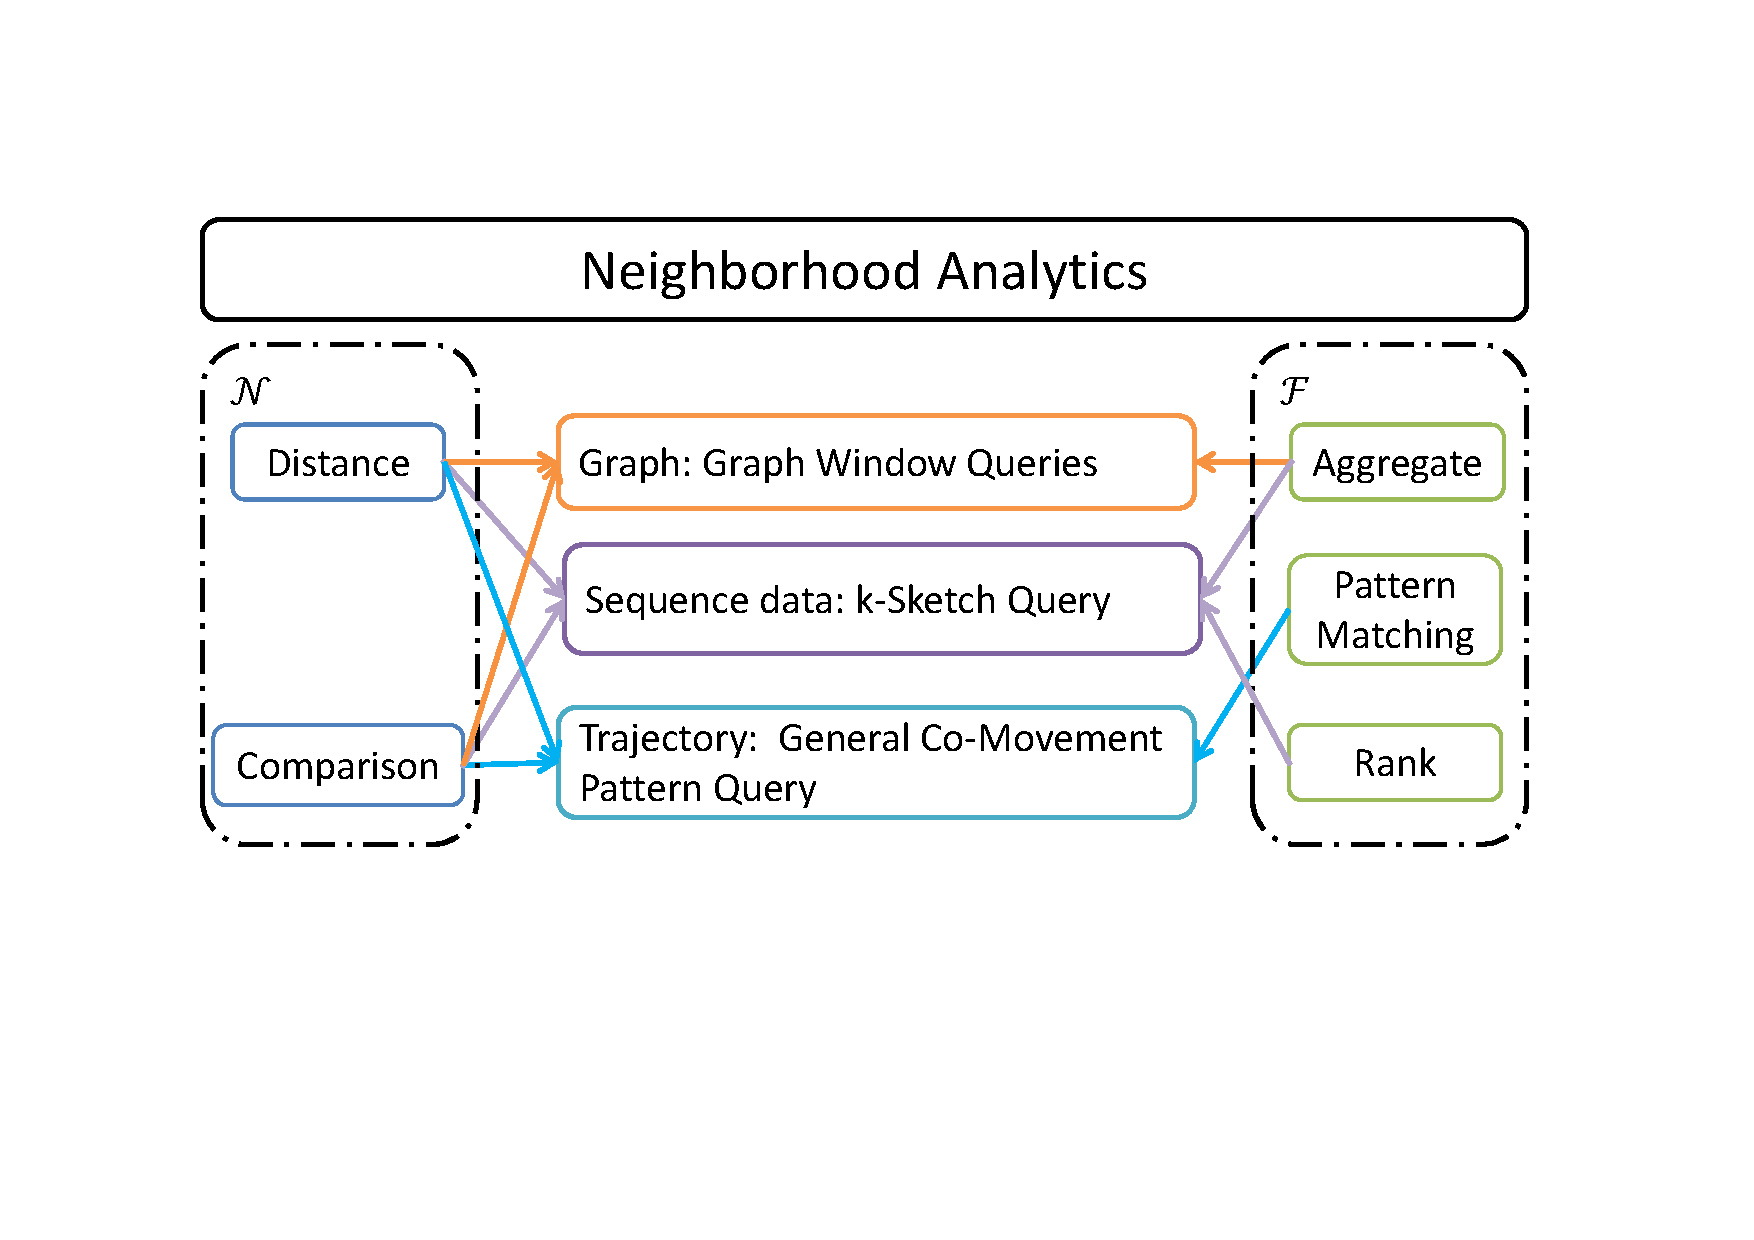
\includegraphics[width=0.8\linewidth]{thesis_roadmap.pdf}
\caption{The roadmap of this thesis. There are three major contributions as highlighted in the center. Each contribution
is an application based on neighborhood analytics with $\mathcal{N}$ and $\mathcal{F}$ as indicated by arrows.} 
\label{fig:thesis_roadmap}
\end{figure}

In a nutshell, we propose three neighborhood based queries in respective data domains. 
In \emph{graph}, we define the Graph Window Query which summarizes the vicinity of each vertex.
The query utilizes both distance neighborhood and comparison neighborhood to facilitate both
general graphs and direct acyclic graphs.
%
%two types of queries: \emph{k-hop window query} is based on the \emph{distance} neighborhood
%and \emph{topological window query} is based on the \emph{comparison} neighborhood. 
In \emph{sequence data}, we propose a $k$-Sketch Query to summarize a subject's history. The $k$-Sketch query builds on a nested \emph{distance} and \emph{comparison} neighborhood based pattern called \emph{rank-aware streak}.
%
% we design a nested \emph{distant} and \emph{comparison} neighborhoods based pattern called \emph{rank-aware streak}, and propose a $k$-Sketch query to select the most representative rank-aware streaks.
In \emph{trajectory}, we propose a General Co-movement Pattern (GCMP) query to discover co-moving behaviors among moving objects. The GCMP query leverages the neighborhood notion to unify existing co-moving patterns in the literature.
%
%we analyze existing movement patterns based
%on \emph{distance} and \emph{comparison} neighborhoods and unify
%the existing works with a general pattern discovery query. 
In the following parts of this section, we present our contributions in detail.


\subsection{Graph Window Queries}
The first piece of the thesis deals with neighborhood analytics
on graph data. Nowadays information network are typically
modeled as attributed graphs where the 
vertexes correspond to objects and the edges capture the
relationships among these objects. As vertexes embed a wealth
of information (e.g., user profiles in social networks), there are 
emerging demands on analyzing these data to extract useful insights. 
We propose the concept of \emph{window analytics} 
for attributed graph and identify two types of such analytics as shown in the following examples:

\textbf{$k$-hop Window:} The $k$-hop neighbors of a vertex form
its $k$-hop window. Since the $k$-hop neighbors are the most structurally
relevant vertexes to the vertex, analytics on the information from the $k$-hop window
would be beneficial. Typical analytic queries include summarizing the related connections' distribution among different companies, and computing age distribution of the related friends can be useful.
%In a social network (such as LinkedIn and Facebook etc.), users are normally modeled as vertexes and connectivity relationships are modeled as edges. In the social network scenario, it is of great interest to summarize the most relevant connections to each user such as the neighbors within $2$-hops. Some analytic queries such as summarizing the related connections' distribution among different companies, and computing age distribution of the related friends can be useful. In order to answer these queries, collecting data from every user's neighborhoods within 2-hop is necessary.
%\end{example}

\textbf{Topological Window:} The topological neighbors are defined
in the context of Directed Acyclic Graph (DAG). In DAGs,
topological neighbors are composed of all the ascendant vertexes of a vertex. 
The topological neighbors represent the most influential vertexes of a given vertex.
Since DAGs are often found in biological networks, topological window would
be helpful to analyze the statistics of molecules of each biological protein's pathway.
%Since the topological neighbors , analytics
%on the topological window would benefit the deeper understanding of the 
%network.
%DAGs are often found
%in biological networks and citation networks. 
% The topological neighbors
%represent the influences from the source vertex to the given vertex, thus
%analytics over topological window would be interesting.

%\begin{example}[Topological window]
%In biological networks (such as Argocyc, Ecocyc etc.), genes, enzymes and proteins are vertexes and their
%dependencies in a pathway are edges. Because these networks are directed and acyclic, 
%in order to study the protein regulating process, one may be interested to find out the statistics of molecules in each protein production pathway. For each protein,we can traverse the 
%graph to find every other molecules that are in the upstream of its pathway.
%Then we can group and count the number of genes and enzymes among those molecules.
%\end{example}

The two \emph{windows} shown in the above examples are essentially neighborhood functions defined for each vertex. Specifically, let $G=(V,E,A)$ be an attributed graph, where $V$ is the set of vertexes, $E$ is the set of edges, and each vertex $v$ is associated as a multidimensional point $a_v \in A$ called attributes.
The \emph{k-hop} window is a \emph{distance} neighborhood function, 
i.e., $\mathcal{N}_1(v,k)= \{u|\mathtt{dist}(v,u) \leq k\}$, 
which captures the vertexes that are $k$-hop nearby. 
The \emph{topological} window,  $\mathcal{N}_2(v)= \{u | u \in v.ancestor\}$,
is a \emph{comparison} neighborhood function that captures
the ancestors of a vertex in a directly acyclic graph.  The analytic function $\mathcal{F}$ is an aggregate function ($\mathtt{sum}$, $\mathtt{avg}$, etc.) on $A$.

Apart from demonstrating the useful use cases on these two windows, 
we also investigate how Graph Window Query processing can be efficiently supported.  We propose
two different types of indexes: Dense Block Index (DBIndex)
and Inheritance Index (I-Index). The DBIndex and I-Index
are specially optimized to support $k$-hop window and topological
window processing. These indexes
integrate the aggregation process with partial work sharing techniques
to achieve efficient computation.
In addition, we develop space and performance efficient techniques
for the index construction. Notably, DBIndex saves upto 80\%
of the index construction time as compared to the state-of-the-art competitor and up to 10 times
speedup in query processing. 


\subsection{$k$-Sketch Query on Sequence Data}
The second piece of this thesis explores the neighborhood analytics on sequence data. 
%In sequence data analysis, 
As part of the sequence data analysis,
summarizing a subject's history with sensational patterns
is an important and revenue-generating task in a plethora of applications 
such as computational journalism~\cite{cohen2011computational,zhang2014discovering}, automatic fact checking~\cite{hassan2014data,walenz2014finding}, and perturbation analysis~\cite{Walenz:2016:PAD:3007328.3007330}.
%
%an important and revenue-generating task is to
%summarize a subject's history using sensational patterns.
An outstanding example of such patterns is the \emph{streak}~\cite{zhang2014discovering},
which is commonly found in stock
and sports reports. For instance:

%For example, streaks may be of the following forms in stock and sports scenarios:

%Streak is commonly used in many sequenced applications,
%such as network monitoring, stock analysis
%and sport reporting. For example, streaks may be of the following forms in stock and sports scenarios:
\begin{enumerate}
	\item{[STOCK]:``Apple Inc.~has an \emph{average} price of USD 115.5 in the \emph{last week}''}
	\item{[SPORTS]: ``Kobe has scored \emph{at least} 60 points in \emph{three straight games}'' }
\end{enumerate}
In general, a streak is constructed from two concepts: an \emph{aggregate function} (e.g., $\mathtt{avg}$, $\mathtt{min}$)
applied on \emph{consecutive events} (e.g., seven days, three games). 
%Indeed, a streak an be simply modeled as a neighborhood query.
However, the streak itself does not embed the strikingness information, which is limited
to represent a sensational pattern. 
%
%
%is a neighborhood query defined for an event where the neighborhood range is the window the event belongs to.
%%
%, a \emph{streak} can be modeled as a neighborhood query
%of events, where the neighborhood function is defined as windows.
%This makes the streak as a neighborhood query of events where the neighborhood function is defined as time windows.
%
%Since the streak is aggregated based on the
%closeness of events in the time domain (i.e., time window), it can be viewed as a neighborhood query where the neighborhood function is defined by the time distance, and the analytic function can be any aggregate function.
%However, it is challenging to directly leverage streaks to discover sensational patterns because
%the strikingness of a streak is missing.
%A direct challenge in discovering phenomenal patterns using streak is
%how to quantify the strikingness of a streak.
For example, \emph{Streak 2} would not be striking if all NBA players were able to score over 60 points. 
On the contrary, knowing that most NBA players only score 20 points in a game,
\emph{Streak 2} is indeed quite striking. 
Therefore, the strikingness of a streak should be measured by comparing with other streaks.
Based on this observation, we propose a rank-aware pattern named \emph{ranked-streak} which measures the strikingness of
a streak by comparing among all streaks under the same condition (i.e., streak length).

Technically, the ranked-streak can be viewed as a joint neighborhood function. 
Let $t_s(e)$ be the sequence number of the event $e$ in the history of subject $s$.
%Let $e_s(t)$ denote the event of subject $s$ at time $t$. 
Then the ranked-streaks of length $L$ are generated using neighborhood functions in a two-step manner: 

\begin{enumerate}
\item {a \emph{distance neighborhood} $\mathcal{N}_1(s,e,L)=\{e_j | t_s(e) - t_s(e_j) \leq L \}$ groups a consecutive $L$ events for each event in the history of subject $s$. Let $\overline{v}$ be the aggregate value associated with $\mathcal{N}_1$, then the output of this step is a set of \emph{streak}s of the form  $sk=\langle s, L, t, \overline{v} \rangle$.}
\item {a \emph{comparison neighborhood} $\mathcal{N}_2(sk) = \{sk_i | sk.L = sk_i.L \wedge sk_i.\overline{v} \geq sk.\overline{v} \}$ ranks a subject's streak among all other streaks with the same length.  Note that the rank information can be simply calculated from a $\mathtt{count}$ function. The result of this step is a tuple $\langle s, L, t, \overline{v}, r \rangle$, where $r$ is the \emph{rank}.}
\end{enumerate}
%(1) a \emph{distance neighborhood} $\mathcal{N}_1(o_i,w)=\{o_j | o_i.t - o_j.t \leq w \}$ groups a consecutive $w$ events for each event. Let $\overline{v}$ be the aggregate value associated with $\mathcal{N}_1$, then the output of this step is a set of \emph{streak}s of the form  $n=\langle o_i, w, t, \overline{v} \rangle$.
%
%(2) a \emph{comparison neighborhood} $\mathcal{N}_2(n_i) = \{n_j | n_j.w = n_i.w \wedge n_i.\overline{v} \geq n_j.\overline{v} \}$ ranks a subject's streak among all other streaks with the same window length. The result of this step is a tuple $\langle o_i, w, t, r \rangle$, where $r$ is the \emph{rank}.
%

As the ranked-streak contains the relative position of the streak among its cohort, it provides a quantitative measure of the strikingness.
For example, the rank-aware version of \emph{Streak 2} would be ``Kobe has scored at least 60 points in three straight games, which is best in the league''.  This clearly suggests that \emph{Streak 2} is striking.
%

On the basis of the ranked-streaks, we study the problem of effectively summarizing
a subject history. We notice that, for a subject with $n$ events, there
are $O{n \choose 2}$ streaks. 
In real life, ``Kobe'' has played $1,000$ games which may produce near half million streaks.
Such a large number of streaks is too overwhelming to represent a subject's history. Hence,
we are motivated to propose a $k$-Sketch query that selects $k$ ranked-streaks which best represent
a subject's history. To find the qualified streaks, we design a novel scoring which
considers both the events covered of the streaks and the ranks of the streaks.
% under a novel scoring function. Our scoring function
%considers both the events covered of the streaks and the ranks of the streaks.

%A prominent drawback of streak is that the amount of streaks
%%Another challenge  the pattern discovery is that the amount of streaks
%for a subject is huge. For a subject with $N$ events,
%there are $O{N\choose 2}$ streaks as well as rank-aware streaks. 
%In real life, ``Kobe'' has played $1000$ games which may produce near half million streaks.
%Such a large number clearly poses difficulties for pattern discoveries.
%%for selecting phenomen streaks. 
%Nevertheless, we observe that many streaks share almost identical information. For example, when Kobe scored 81 points
%in one game, this single-event streak ranks number 1 among all streaks. Subsequently, the streaks with size 3 (i.e., 3 straight games afterwards) ranked number 10. Thus reporting this
%streak only provide redundant striking information (i.e., the 81 point game).
%Based on this observation, we
%propose a $k$-Sketch query to select the $k$ most \emph{representative streaks} via a novel scoring function that considers both strikingness and diversity of streaks.
%
%Our $k$-Sketch query is based on a novel scoring function that consider both the 
%stringness and the diversity of the streaks. 

In this thesis, we extensively study
the technical issues in processing $k$-Sketch queries in both online and offline scenarios.
In the offline scenario, we design two pruning techniques which largely
reduce the streaks enumerated in generating ranked-streaks. Then, we adopt a
$(1-1/e)$-approximate sketch selection algorithm by utilizing the 
submodularity of the $k$-Sketch query. In the online scenario, we design
an \emph{online-streak bound} to avoid evaluating many unnecessary streaks. Furthermore,
we propose a $1/8$-approximate algorithm to facilitate efficient sketch maintenance.
In the experimental study, we compare our solutions with baselines using
four real datasets, and the results demonstrate the efficiency and 
effectiveness of our proposed algorithms: the running time
achieves up to 500 times speedup as compared to the baseline and the quality of the
detected sketch is endorsed by the anonymous users
from Amazon Mechanical Turk\footnote{\url{https://requester.mturk.com}}. 
%
%, our techniques is confirmed by the experiments on four 
%real datasets. And the effectiveness of our $k$-Sketch query is endorsed
%by the anonymous users from Amazon Mechanical Turk\footnote{\url{https://requester.mturk.com}}.

%%
%%Besides proposing the rank-aware streak, we also technically 
%%study how to efficiently support the \emph{$k$-Sketch} query in both
%%offline and online scenarios. We propose various window-level 
%%pruning techniques to find striking candidate steaks.
%%Among those candidates, we then develop approximation
%%methods, with theoretical bounds, to discover $k$-sketches for each subject. 
%Furthermore, we conduct experiments on four real
%datasets, and the results demonstrate the efficiency and 
%effectiveness of our proposed algorithms: the running time
%achieves up to 500x speedup as compared to baseline and the quality of the
%detected sketch is endorsed by the anonymous users
%from Amazon Mechanical Turk \footnote{\url{https://requester.mturk.com}}.

\subsection{Co-Movement Pattern Query on Trajectory Data}
The third piece of the thesis studies the neighborhood
analytics in the trajectory domain. 
In trajectory analysis, an important
mining task is to discover traveling patterns among moving objects. 
A traveling pattern is often determined by the spatial neighborhoods of moving objects. One of the prominent examples is the \emph{co-movement pattern}~\cite{li2013onlinegroup,zheng2015trajectory}.
A co-movement pattern refers to a group of moving objects traveling together for a certain period of time. 
We observe that the co-movement pattern can be concisely represented using two neighborhood functions in spatial and temporal domains as follows:

%Table~\ref{tbl:intro-move-patterns} summarizes several popular co-movement patterns with different 
%constraints with respect to clustering in spatial proximity, consecutiveness in temporal duration
%and computational complexity. In particular, the flock~\cite{gudmundsson2006computing} and the group~\cite{wang2006grouppattern} patterns require all the objects in a group to be enclosed by a disk with radius $r$;
%whereas the convoy~\cite{jeung2008discovery}, the swarm~\cite{li2010swarm} and the platoon~\cite{li2015platoon} patterns resort to density-based spatial clustering. In the temporal dimension,
%the flock~\cite{gudmundsson2006computing} and the convoy~\cite{jeung2008discovery} require all the timestamps
%of each detected spatial group to be consecutive, which is referred to as global consecutiveness; whereas the swarm~\cite{li2010swarm} does not impose any restrictions. 
%The group~\cite{wang2006grouppattern} and the platoon~\cite{li2015platoon} adopt 
%a compromised approach by allowing arbitrary gaps between consecutive segments, 
%which is called local consecutiveness. They introduce a parameter $L$ to control the minimum length of each local consecutive segment.
%
%
%\begin{table}[h]
%\centering
%\begin{tabular}{|l|c|c|}
%\hline 
%\textbf{Pattern} & {\textbf{Proximity}} & { \textbf{Consecutiveness}} \\% & { \textbf{Time  Complexity}}\\ 
%\hline 
%flock~\cite{gudmundsson2006computing} & disk based &  global \\%& {$O(|\mathbb{O}||\mathbb{T}|\log(|\mathbb{O}|))$} \\ 
%\hline 
%convoy~\cite{jeung2008discovery} & density based &   global \\%& {$O(|\mathbb{O}|^2+|\mathbb{O}||\mathbb{T}|)$}\\ 
%\hline 
%swarm~\cite{li2010swarm} & density based  & - \\%& {$O(2^{|\mathbb{O}|}|\mathbb{O}||\mathbb{T}|)$}  \\ 
%\hline 
%group~\cite{wang2006grouppattern} & disk based &  local \\%& {$O(|\mathbb{O}|^2|\mathbb{T}|)$}\\ 
%\hline 
%platoon~\cite{li2015platoon} & density based &  local \\%& {$O(2^{|\mathbb{O}|}|\mathbb{O}||\mathbb{T}|)$}\\ 
%\hline 
%\end{tabular} 
%\caption{Constraints of co-movement patterns.}
%\label{tbl:intro-move-patterns}
%\end{table}
%Neighborhoods relationship
%among moving objects forms the traveling behavior of the objects
%which is often referred as moving patterns. Specifically, the neighborhoods
%of objects are defined based on the spatial proximity and the 
%
%
%nIn trajectory domain, an instance 
%of neighborhood usage is to detect the movement pattern. In simple
%words, a movement pattern is a set of moving object whose trajectories
%exhibits interesting behaviors.
%
%Due to its wide spectrum of applications, 
%mining the movement patterns have attracted many research attention.

%
%In trajectory domain, the neighborhoods of objects across multiple time snapshots collectively 
%form a movement pattern. Due to its wide spectrum of applications, mining the movement patterns have attracted many research attention.
%
%In the trajectory domain, neighborhood
%functions can effectively model the movement patterns
%of objects which is useful in a wide
%spectrum of applications. 
%
%An important mining task in trajectory
%data that has drawn many research attention is discovering
%movement patterns. Coincidentally, a movement pattern
%can be 
%
%
%Discovering co-movement patterns from large-scale trajectory 
%databases is an important mining task and has a wide
%spectrum of applications. 
%Existing studies have identified several types of interesting movement patterns called \emph{co-movement} patterns. A co-movement pattern refers to a group of moving objects traveling together for a certain period of time and the group of objects is normally determined by their spatial proximity. A pattern is prominent if the group size exceeds $M$ and the length of duration exceeds $K$. 
%Inspired by the basic definition 
%and driven by different mining applications, there are a bunch of variant 
%co-movement patterns that have been developed with more advanced constraints.

%\begin{figure}[h]
%\centering
%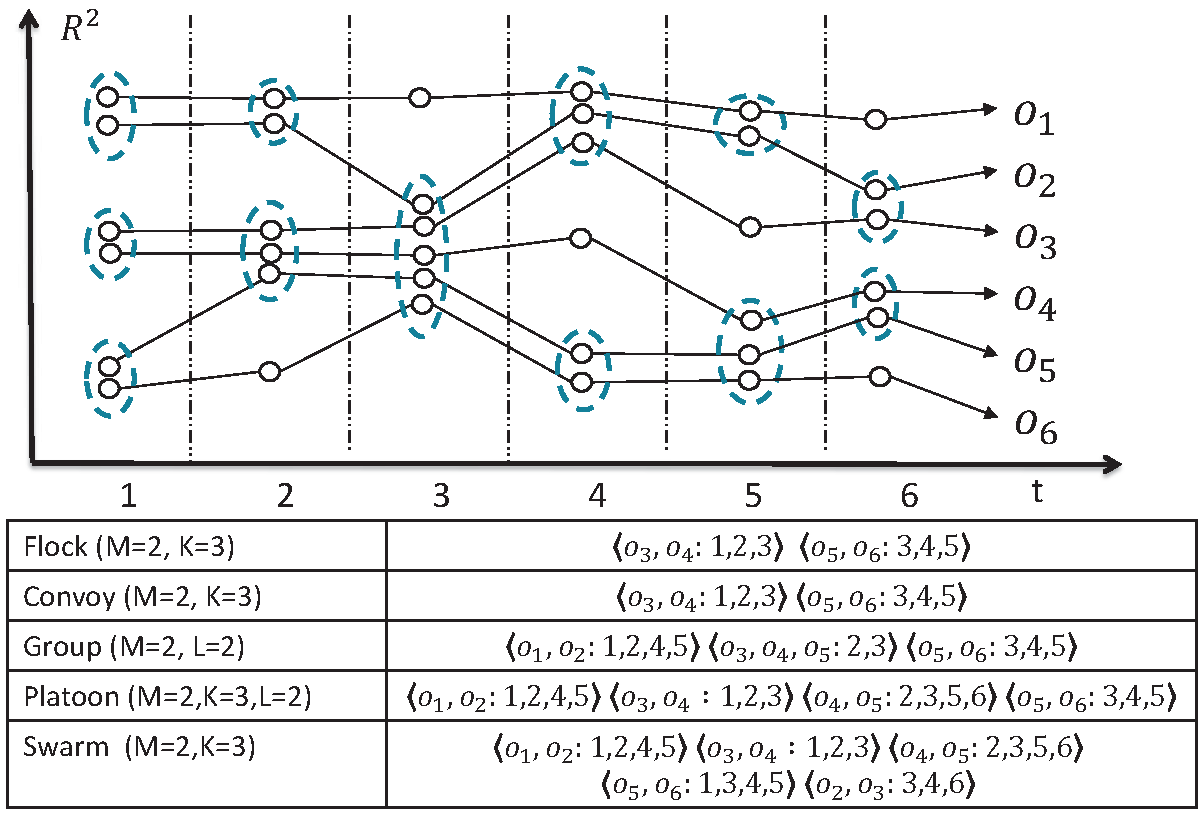
\includegraphics[width=0.8\textwidth]{trajectory_patterns.pdf}
%\caption{Trajectories and co-movement patterns. The example consists of six trajectories across six snapshots. Objects in spatial clusters are enclosed by dotted circles. $M$ is the minimum cluster cardinality; $K$ denotes the minimum number of snapshots for the occurrence of a spatial cluster; and $L$ denotes the minimum length for local consecutiveness.}
%\label{fig:related_work}
%\end{figure}
%
%Figure~\ref{fig:related_work} is an example to demonstrate the concepts of various co-movement patterns. The trajectory database consists of six moving objects and the temporal dimension is discretized into six snapshots. In each snapshot, we treat the clustering method as a black-box and assume that they generate the same clusters. Objects in proximity are grouped in the dotted circles. As aforementioned, there are three parameters to determine the co-movement patterns and the default settings in this example are $M=2$, $K=3$ and $L=2$. Both the \emph{flock} and the \emph{convoy} require the spatial clusters to last for at least $K$ consecutive  timestamps. Hence,$\langle o_3,o_4:1,2,3 \rangle$ and $\langle o_5,o_6:3,4,5 \rangle$  remains the only two candidates matching the patterns. The \textit{swarm} relaxes the pattern matching by discarding the temporal consecutiveness constraint. Thus, it generates many more candidates than the \textit{flock} and the \textit{convoy}. The \textit{group} and the \textit{platoon} add another constraint on local consecutiveness to retain meaningful patterns. For instance, $\langle o_1,o_2:1,2,4,5 \rangle$ is a pattern matching local consecutiveness because timestamps $(1,2)$ and $(4,5)$ are two segments with length no smaller than $L=2$. The difference between the \textit{group} and the \textit{platoon} is that the \textit{platoon} has an additional parameter $K$ to specify the minimum number of snapshots for the spatial clusters. This explains why $\langle o_3,o_4,o_5:2,3 \rangle$ is a \textit{group} pattern but not a \textit{platoon} pattern.


%As shown, there are various types of co-movement patterns facilitating different application needs and 

	(1) In spatial domain, let $o(t)$ be the spatial location of object $o$ at time $t$. The co-moving objects of an object $o$
	can be determined by a \emph{distance neighborhood} $\mathcal{N}_1$. For example,  flock~\cite{gudmundsson2006computing} and group~\cite{wang2006grouppattern} patterns use the \emph{disk-based} clustering, which is equivalent to $\mathcal{N}_1(o, t)= \{o_j | \mathtt{dist}(o(t),o_j(t)) < r \}$. Convoy~\cite{jeung2008discovery}, swarm~\cite{li2010swarm} and platoon~\cite{li2015platoon} patterns use the \emph{density-based} clustering, which is equivalent to $\mathcal{N}_1(o,t)= \{o_j | \mathtt{dist}(o_j(t),o_k(t)) \leq \epsilon \wedge o_k \in \mathcal{N}_1(o,t)\}$.
%	
%	
%	spatial groups of moving objects at time $t$
%	can be formed by a \emph{distance neighborhood} $\mathcal{N}_1$. For example,  flock~\cite{gudmundsson2006computing} and group~\cite{wang2006grouppattern} patterns use the \emph{disk-based} clustering, which is equivalent to $\mathcal{N}_1(o, t)= \{o_j | \mathtt{dist}(o(t),o_j(t)) < r \}$. Convoy~\cite{jeung2008discovery}, swarm~\cite{li2010swarm} and platoon~\cite{li2015platoon} patterns use the \emph{density-based} clustering, which is equivalent to $\mathcal{N}_1(o,t)= \{o_j | \mathtt{dist}(o_j(t),o_k(t)) \leq \epsilon \wedge o_k \in \mathcal{N}_1(o,t)\}$.
%	
%	 $\mathcal{N}_1$ is a \emph{distance neighborhood} used to determine the spatial proximity of objects. For example,  flock~\cite{gudmundsson2006computing} and group~\cite{wang2006grouppattern} patterns uses the \emph{disk-based} clustering, which is equivalent to $\mathcal{N}_1(o, t)= \{o_j | \mathtt{dist}(o(t),o_j(t)) < r \}$ for each object. Convoy~\cite{jeung2008discovery}, swarm~\cite{li2010swarm} and platoon~\cite{li2015platoon} patterns uses the \emph{density-based} clustering, which is equivalent to $\mathcal{N}_1(o,t)= \{o_j | \mathtt{dist}(o_j(t),o_k(t)) \leq \epsilon \wedge o_k \in \mathcal{N}_1(o_i,t)\}$.
	
	(2) In temporal domain, objects that co-move with $o$ for a duration $T$ can be determined by
	a \emph{comparison neighborhood} $\mathcal{N}_2$:
% is a \emph{comparison neighborhood} used to determine co-moving behavior, i.e.,
	%objects that co-move with $o$ for a duration $T$ can be represented by 
	$\mathcal{N}_2(o, T)=\{o_j| \forall t \in T, o_j \in \mathcal{N}_1(o,t) \}$.%, where $C_t(\cdot)$ returns the neighborhoods (i.e., $N_1$) of an object at time $t$.

A pattern is deemed significant if the group size exceeds $M$ (i.e., $|\mathcal{N}_2(\cdot)| \geq M$ and the length of duration exceeds $K$ (i.e., $T \geq K$). 
%The group is defined based on the spatial proximity of objects, which 
%can be seen as the spatial neighbors of each object.
%
%
Rooted from the basic movement definition and driven by different mining applications, there are several instances of co-movement patterns that have been developed with more advanced constraints, namely \emph{flock}~\cite{gudmundsson2006computing}, \emph{convoy}~\cite{jeung2008discovery}, \emph{swarm}~\cite{li2010swarm}, 
\emph{group}~\cite{wang2006grouppattern} and \emph{platoon}~\cite{li2015platoon}. 
However, these solutions are tailored for each individual pattern and it is cumbersome to deploy and optimize each of the algorithms in real applications. Therefore, there 
calls for a general framework which provides versatile and efficient support on these pattern discoveries. 


Towards this goal, we propose a \emph{General Co-Movement Pattern} (GCMP)
query to capture all existing co-movement patterns in one shot. In GCMP, we treat the proximity detection (i.e., $\mathcal{N}_1$) as
a black box and only focus on the pattern detection (i.e., $\mathcal{N}_2$). We relax the parameter settings on the
co-moving duration (i.e., $T$) and by tuning different parameters (as explained in later sections), GCMP
query is able to detect any of the existing patterns.
%
%It is notable that the GCMP
%query is able to detect any of the existing co-movement patterns by adopting different analytic functions.



In the technical aspect, we study how to efficiently process GCMP query 
on the modern parallel processing platform (i.e., Apache Spark) to
gain scalability over large-scale trajectories. 
In particular, we propose two parallel frameworks: (1) TRPM, which partitions trajectories by replicating snapshots in the temporal domain. Within each partition, a line-sweep method is developed to find all patterns. 
(2) SPARE, which partitions trajectories based on object's neighborhood. Within each partitions, a variant of Apriori enumerator is applied to generate all patterns. 
We deploy the two solutions in our in-house cluster with 11 machines. The experiments on three
real trajectory datasets up to 170 million data points confirm the scalability and efficiency 
of our methods.
%
%We then show the efficiency of both our methods in the Apache Spark platform with three real trajectory datasets upto 170 million points. The results show that SPARE achieves upto 14 times efficiency as compared to TRPM, and 112 times speedup as compared to the state-of-the-art centralized schemes.


\section{Thesis Organization}
The remaining part of the thesis are organized as follows: in Chapter 2, we summarize related literature on neighborhood related analytics in different data domains. In Chapter 3, we present the window function on graph data. In Chapter 4, we present a news discovery application on time series data.
In Chapter 5, we present a pattern mining framework on trajectory data. Chapter 6 summarizes this thesis and highlights the future directions.

\chapter{Literature Review}

Lorem ipsum dolor sit amet, consectetur adipiscing elit, sed do eiusmod tempor incididunt ut labore et dolore magna aliqua. Ut enim ad minim veniam, quis nostrud exercitation ullamco laboris nisi ut aliquip ex ea commodo consequat. Duis aute irure dolor in reprehenderit in voluptate velit esse cillum dolore eu fugiat nulla pariatur. Excepteur sint occaecat cupidatat non proident, sunt in culpa qui officia deserunt mollit anim id est laborum.
\chapter{Graph Window Query: Neighborhood Analytics on Attributed Graphs}

%\section*{Preface}
%Nowadays, attributed graph are prevalently adopted to model
%linked data in many applications, such as social networks and biological networks.
%Besides the link structure, attributed graph also captures
%the attribute information of vertexes. In such a graph domain,
%vertexes are the objects of interest. Therefore, the natural definition of
%neighborhoods would base on the interconnections between the vertexes.
%In this chapter, we introduce the Graph Window Query, which encloses two neighborhood
%definitions. The $k$-hop neighborhood is a distance neighborhood, and the
%topological neighborhood is a comparison neighborhood. We first present the 
%semantic of these two window queries and then
%discuss how to 
%efficient process graph window queries in large-scale graphs.

\section{Introduction}
Information networks such as social networks, 
biological networks and phone-call networks are 
typically modeled as graphs \cite{chen2008graph}
where the vertexes correspond to objects and the edges
capture the relationships between these objects.
For instance, in social networks, every user is represented by
a vertex and the friendship between two users is reflected by an edge between
the vertexes. In addition, a user's profile can be maintained as
the vertex's attributes. Such graphs contain a wealth of valuable 
information which can be analyzed to discover interesting patterns. 
For example, we can find the top-k influential users who can 
reach the most number of friends within 2 hops. With increasingly
larger network sizes, it is becoming significantly challenging to 
query, analyze and process these graph data. Therefore, there is an urgent need 
to develop effective and efficient mechanisms over graph data to draw out
information from such data resources.
 
Traditionally, in relational DBMS, window functions have been commonly
used for data analytics \cite{cao2012optimization, bellamkonda2013adaptive}. 
Instead of performing analysis (e.g., ranking, aggregate) over the entire data set, 
a window function returns for each input tuple a value derived from applying the function over a window of 
neighboring tuples. For instance, users may be interested in finding 
each employee's salary ranking within the department. Here,
each tuple's neighbors are essentially records from the same department.

%Interestingly, we find that the locality feature in graph scenario has even more importance than in relational data. In graph data, the graph structure indicates the relationship among different objects. In graph analysis, it is often useful to quantify a structural range to each vertex and perform analytic over the range. For instance, in a social network, it is important to detect one person's social position and influence in his/her social community. In this paper, we are motivated to extend the window queries in traditional SQL into the graph analysis. However, the window definition in the SQL is no longer applicable in graph context, as it does not capture the graph structure information which has a strong meaning in the graph data. 

Interestingly, the notion of window functions turns out to be not uncommon
in graph data. For instance, in a social network, it is important to detect 
a person's social position and influence among his/her social community. 
The ``social community'' of the person is essentially his/her ``window'' 
comprising neighbors derived from his/her k-hop friends.
However, as illustrated in this example, the structure of a graph
plays a critical role in determining the neighboring data of a vertex.
In fact, it is often useful to quantify a structural range to each vertex 
and then perform analytics over the range. 
Surprisingly, though such a concept of window functions has been widely
used, the notion has not been explicitly formulated. 
In this paper, we are motivated to extend the window queries in traditional 
SQL for supporting graph analysis. However, the window definition in 
SQL is no longer applicable in a graph context, as it does not capture 
the graph structure information.
% which has a strong meaning in the graph data. 
Thus, we seek to formulate the notion of graph windows and to develop
efficient algorithms to process them over large scaled graph structures. 

We have identified two instances of graph windows, namely 
$k${\em -hop} and {\em topological} windows. 
We first demonstrate these window semantics with the following examples. 
\begin{example}
\label{query:linkedin-2-hop-window}
\emph{(k-hop window)} In a social network ( such as Linked-In and Facebook etc.), users are normally modeled as vertexes and connectivity relationships are modeled as edges. In social network scenario, it is of great interest to summarize the most relevant connections to each user such as the neighbors within 2-hops. Some analytic queries such as summarizing the related connections' distribution among different companies, and computing age distribution of the related friends can be useful. In order to answer these queries, collecting data from every user's neighborhoods within 2-hop is necessary.
\end{example}

\begin{example}
\label{query:bio-dag-window}
\emph{(Topological window)} In biological networks (such as Argocyc, Ecocyc etc.\cite{keseler2005ecocyc}), genes, enzymes and proteins are vertexes and their dependency in a pathway are edges. Because these networks are directed 
and acyclic, in order to study the protein regulating process, one may be 
interested to find out the statistics of molecules in each protein 
production pathway. For each protein, we can traverse the graph to find 
every other molecule that is in the upstream of its pathway. Then we can group and count the number of genes and enzymes among those molecules. 
\end{example}

A common feature among these examples is that data aggregation is needed based on a set of vertexes (which is the {\em graph window}) 
defined according to each vertex.  To illustrate, in Example~\ref{query:linkedin-2-hop-window}, every user needs to gather data from its friends and friends-of-friends. 
The \emph{2-hop neighbors} form its window. Likewise, in Example~\ref{query:bio-dag-window}, every protein needs to count the number of particular type of genes preceding it in the regulating pathway. For every protein, the set of
\emph{preceding molecules} forms its window. 

To support the analyses in the above-mentioned examples, we propose a new 
type of query, \emph{Graph Window Query} (GWQ in short),
over a data graph. \emph{GWQ} is defined with respect to a graph structure 
and is important in a graph context. Unlike the traditional window in SQL, 
we identify two types of useful graph windows according to the 
graph structures, namely k-hop Window $W_{kh}$ and Topological Window $W_t$. 
A k-hop window forms a window for one vertex by using its k-hop neighbors. 
k-hop neighbors are important to one vertex, as these are the vertexes 
showing structural closeness as in Example~\ref{query:linkedin-2-hop-window}. The k-hop neighbors window 
we define here is similar to the egocentric-network in network analysis \cite{burt2009structural} \cite{mondal2014eagr}. A topological window, on the
other hand, forms a window for one vertex by using all its preceding 
vertexes in a directed acyclic graph. The preceding vertexes of one vertex are normally those which influence the vertex in a network as illustrated in Example~\ref{query:bio-dag-window}. 

To the best of our knowledge, existing graph databases or graph query languages do not directly support our proposed GWQ. There are two major challenges in processing GWQ. First, we need an efficient scheme to  calculate the window of each vertex. Second, we need
efficient solutions to process the aggregation over a large number 
of windows that may overlap. This offers opportunities to share the 
computation. However, it is non-trivial to address these two challenges.  

For $k$-hop window like query, the state-of-the-art processing algorithm
is EAGR \cite{mondal2014eagr}. EAGR builds an overlay graph including 
the shared components of different windows. This is done 
in multiple iterations, each of which performs the following.
First, EAGR sorts all the vertexes according to their $k$-hop 
neighbors based on their lexicographic order. 
Second, the sorted vertexes are split into equal sized chunks each of which is further built as one frequent-pattern tree to mine the shared components. 
However, EAGR requires all the vertexes' $k$-hop 
neighbors to be pre-computed and resided in memory during 
each sorting and mining operation;
otherwise, EAGR incurs high computation overhead if the pre-computed structure needs to be shuffled to/from disk.
This limits the efficiency and scalability of EAGR.
 For instance, 
a LiveJournal social network graph\footnote{Available at http://snap.stanford.edu/data/index.html, which is used in \cite{mondal2014eagr}} 
(4.8M vertices, 69M edges) generates over 100GB neighborhood information 
for k=2 in adjacency list representation. In addition, the overlay graph construction is not a one-time task,
but periodically performed after a certain number of structural updates in order to maintain the overlay quality. The high memory consumption renders the scheme impractical 
when $k$ and the graph size increases.

In this paper,
we propose \textit{Dense Block Index (DBIndex)} 
to process queries efficiently.
Like EAGR, DBIndex seeks to exploit common
components among different windows to salvage 
partial work done. However, unlike EAGR,
we identify the window similarity utilizing a hash-based 
clustering technique instead of sorting. This ensures 
efficient memory usage, as the window information of each vertex can 
be computed on-the-fly. On the basis of the clusters, we develop different optimizations 
to extract the shared components which result in an efficient index construction. 

Moreover, we provide another \emph{Inheritance Index (I-Index)} tailored 
to topological window query. I-Index differentiates itself from
DBIndex by integrating more descendant-ancestor relationships 
to reduce repetitive computations. This results in
%to reduce the repetitive computation. This results in
more efficient index construction and query processing.  

 
Our contributions are summarized as follows:
\begin{itemize}
\item{We propose a new type of graph analytic query, \emph{Graph Window Query} and formally define two graph windows: k-hop window and topological window. We illustrate how these window queries would help users better query and
understand the graphs under these different semantics.}

\item{ To support efficient query processing, we further propose two different types of indexes: \emph{Dense Block Index} (DBIndex) and \emph{Inheritance Index} (I-Index). The
\emph{DBIndex} and \emph{I-Index} are specially 
optimized to support k-hop window and topological window query processing. 
We develop the indices by integrating the window aggregation sharing techniques to salvage partial work done for efficient computation. In addition, we develop space and performance efficient techniques for index construction. 
Compared to EAGR \cite{mondal2014eagr}, the state-of-the-art index method for k-hop window queries, our DBIndex is much more memory efficient and scalable towards handling the large-scale graphs. }

\item{We perform extensive experiments over both real and synthetic datasets
with hundreds of millions of vertexes and edges on a single machine. Our experiments 
indicate that our proposed index-based algorithms outperform the naive non-index
algorithm 
by up to four orders of magnitude. In addition, our experiments also show 
that DBIndex is superior over EAGR in terms of both
scalability and efficiency. In particular, 
DBIndx saves up to 80\% of indexing time as 
compared to EAGR, 
and performs well even when EAGR fails due
to memory limitations. 
}
\end{itemize}

%\section{Related Work}
%Window function was proposed in \cite{zemke2012s}, which is widely used in SQL data analytic. There are several optimization on standard window functions \cite{cao2012optimization, bellamkonda2013adaptive}. \cite{cao2012optimization} optimize window function via shared sorted components, and \cite{bellamkonda2013adaptive} optimized window function via partition. However, in \emph{GWF}, the sorting and partition is no longer required, thus their techniques are not applicable in the graph window context.
%\remark{We haven't mention GWFs in introduction section, does this needs to be mentioned?}
Our proposed graph window functions (GWFs) for graph databases is inspired by the usefulness of window functions in relational analytic queries
\cite{zemke2012s}.

A window function in SQL typically specifies a set of partitioning attributes $A$ and an aggregation function $f$.
Its evaluation first partitions the input records based on $A$ to compute $f$ for each partition,
and each input record is then associated with the aggregate value corresponding to the partition that contains the record.
Several optimization techniques \cite{cao2012optimization, bellamkonda2013adaptive}
have also been developed to evaluate complex SQL queries involving multiple window functions.
%by reducing the overall partitioning cost to evaluate the aggregation functions.
%\remark{Need to also cite an earlier Oracle tech report.}

%However, in \emph{GWF}, the sorting and partition is no longer required, thus their techniques are not applicable in the graph window context.
However, the semantics and evaluation of window functions are very different between relational and graph contexts.
Specifically, the partitions (i.e., subgraphs) associated with GWFs are not necessarily disjoint; thus,
the evaluation techniques developed for relational context \cite{cao2012optimization, bellamkonda2013adaptive} are not applicable to GWFs. %\remark{\cite{bellamkonda2013adaptive} focuses on utilizing partition to parallel window processing, and \cite{cao2012optimization} focuses on leveraging sorting among windows. However sorting and partitioning are no longer exists in GWFS, thus, their work are not applicable}

GWFs are also different from graph aggregation \cite{zhao2011graph,wang2014pagrol,chen2008graph,tian2008efficient} in graph OLAP.
In graph OLAP, information in a graph are summarized
by partitioning the graph's nodes/edges (based on some attribute values) and computing aggregate values for each partition.
GWFs, on the other hand, compute aggregate values for each graph node w.r.t. the subgraph associated with the node.
Indeed, such differences also arise in the relational context, where different 
techniques are developed to evaluate OLAP and window function queries.

In \cite{yan2010top}, the authors investigated the problem of finding the vertices that have top-k highest aggregate values over their h-hop neighbors. They proposed mechanisms to prune the computation by using two properties: First, the locality between vertices is used to propagate the upper-bound of aggregation; Second, the upper-bound value of aggregates can be estimated from the distribution of attribute values. However, all these pruning techniques are not applicable in our work, as we need to compute the aggregation value for every vertex. In such a scenario, techniques in \cite{yan2010top} degrade to the non-indexed approach as described in Section 4.
%rather than finding the top-k values.  

%\cite{cheng2012k} provided a \emph{K-Reach} index for fast determining whether two vertices can be reached within K-hop distance. However, \emph{K-Reach} index can not be directly used to support the k-hop window query due to its high overhead. Gathering the window of one vertex may involve $|V|$ reachability detections which results in the complexity of $O(|V|^2)$ to compute the windows for all the vertices, where $|V|$ is the number of vertices.}  

Indexing techniques have been proposed to efficiently determine whether an input pair of vertices is within a distance of k-hops (e.g. k-reach index \cite{cheng2012k}) or reachable (e.g. reachability index \cite{yu2010graph}). However, such techniques are not efficient for computing the k-hop window or topological window for a set of $n$ vertices with a time complexity of $O(n^2)$. 



%Indexing techniques \cite{yu2010graph,cheng2012k} is able to test whether a vertex belongs to another vertex's window. \cite{cheng2012k} proposed \emph{K-Reach} index which tests a whether an input pair of vertices is within a distance of k-hops, thus it can be used to compute \emph{k-hop} window. \cite{yu2010graph} surveys a wealth of \emph{Reachability Indices} which tests whether a input pair of vertices is reachable, thus it can be used to compute \emph{topological} window. However, those techniques are not efficient for computing either \emph{k-hop} or \emph{topological} window, since for a set of $n$ vertices, their complexity of forming window is of $O(n^2)$.

% which efficiently determines whether an input pair of vertices is within a distance of k-hops. Thus \emph{K-Reach} is able to facilitate \emph{k-hop} window. While, \cite{yu2010graph} presents a survey of reachability indices which determine whether an input pair of vertices is connected. Thus, those techniques is able to facilitate \emph{topological} window. However, such techniques are not efficient for computing either \emph{k-hop} or \emph{topological} window, since for a set of $n$ vertices, their complexity of forming window is of $O(n^2)$.

%Indexing techniques such as the \emph{K-Reach} index \cite{cheng2012k} have been proposed
%to efficiently determine whether an input pair of vertices is within a distance of k-hops.  
%However, such techniques are not efficient for computing the k-hop window for a set of $n$ vertices has a time complexity of $O(n^2)$.

%However, \emph{K-Reach} index can not be directly used to support the k-hop window query due to its high overhead. Gathering the window of one vertex may involve $|V|$ reachability detections which results in the complexity of $O(|V|^2)$ to compute the windows for all the vertices, where $|V|$ is the number of vertices.}  
%
%use \emph{K-Reach} index to collect the windows of each vertex 
%
%it incurs high overhead to adopt \emph{K-Reach} index to gather the window for a k-hop window query. The reason is that  
%
%is unable to answer k-hop window query. To see this, for each vertex, $|V|$ reachability queries need to be performed in order to gather a window. The total running time of this approach is $O(|V|^2|R|)$, where $|R|$ is the cost for answering one reachability query. This is obvious not acceptable in terms of query performance.

\eat{\cite{mondal2014eagr} proposed an EAGR system which evaluates neighborhood-based aggregation
queries over low hops (k = 1). They follow a in-memory model and assume the k-hop information 
for each vertex is pre-computed. Based on the neighborhood information, it first sort each vertex
using lexicographic order. Then vertices are split into equal sized chunks. For each chunk, it 
then builds a Frequent-Pattern Tree for iteratively mining the shared components between each vertex's 
neighborhoods. Lastly, it builds an overlay graph based on the shared components for efficient computing.
}

\cite{mondal2014eagr} proposed an EAGR system, which uses the famous VNM heuristic and Frequent-Pattern
Tree to find the shared component among each vertex's neighborhoods. It starts by building an
overlay graph as a bipartite graph representing the vertex-neighbor mapping. Then it aims to
find the bi-cliques in the overlay graph. Each bi-clique represents a set of vertices whose neighborhood
aggregates can be shared. Once a bi-clique is found, it is inserted back to the overlay graph as
a virtual node to remove redundant edges. EAGR find bicliques in iterations. During each iteration,
it sorts each vertices in overlay graph by their neighborhood information. Then the sorted vertices 
are split into equal-sized chunks. For each chunk, it then builds a FP-Tree to mining the large bi-cliques. 
As the algorithm iterates, the overlay graph evolves to be less dense. 


The main drawback of EAGR is its demands of high memory usage on overlay construction. It
requires the neighborhood information to be pre-computed, which is used in the sorting phase
of each iteration. In EAGR the neighborhood information is assumed to be stored in memory.
However, the assumption does not scale well for computing higher hop windows (such as k $\geq 2$). 
For instance, a LiveJournal social network graph \footnote{Available at http://snap.stanford.edu/data/index.html, which is used \cite{mondal2014eagr}} (4.8M nodes, 69M edges) generates over 100GB mapping information for k=2 in adjacency list 
representation. If the neighborhood information is resided in disk, the performance of EAGR will
largely reduced. Similarly, if the neighborhood information is computed on-the-fly, EAGR needs
to perform the computation in each iteration, which largely increases indexing time.

We tackle this drawback by adapting a hash based approach that clusters each vertex based
on its neighborhood similarity. During the hashing, the vertex's neighborhood information
is computed on-the-fly. As compared to sorting based approach, we do not require vertex's neighborhood
to be pre-reside in memory. In order to reduce the repetitive computation of vertex's neighborhood,
we further propose an estimation based indexing construction algorithm that only require a vertex's small
hop neighborhood to be computed during clustering. As our experiments show, our proposed methods 
can perform well even when EAGR algorithm fails when neighborhood information overwhelms system's memory.
To further reduce the neighborhood access, we adapted a Dense Block heuristic process each vertex
in one pass. Experiments shows that the performance of our heuristic is comparable to EAGR's, but with
much shorter indexing time.
  


  

%
%\eat{The work that is most related to ours is 
% \cite{mondal2014eagr} - referred as EAGR 
%which examines the evaluation of neighborhood-based or ego-centric (similar to our k-hop window)
%aggregation queries. 
%Both EAGR and our DBIndex aim to speed up the aggregation computation by sharing the processing of the intersections among different windows. There are, however, two main differences between our work and EAGR.
%First, while both EAGR and our approach are main-memory techniques, 
%our approach is much more memory efficient and scalable than EAGR.
%%which results in a high scalablity to support large-scale graphs. 
%%The scalability limitation of EAGR arises due to its assumption that the mapping information about all vertices' windows must be precomputed and stored in main memory, and memory-inefficient data structure, Frequent Pattern Tree (FPT) adopted to construct the overlay graph. Note that FPT has almost the same high space requirement as the mapping information for a large k: for k-hop queries, in $O(|V|d^k)$ if represented as an adjacency lists and
%The scalability limitation of EAGR arises due to its large memory requirement 
%for both the mapping information for all vertex windows 
%as well as a Frequent Pattern Tree (FPT) data structure used to construct an overlay graph. 
%Each of these main-memory structures
%has a space complexity of $O(nd^k)$ if represented as an adjacency lists and
%$O(n^2)$ if represented as adjacency matrix,
%for $k$-hop queries where $n$ denotes the number of vertices and $d$ denotes the average node degree. 
%For instance, a LiveJournal social network graph \footnote{Available at http://snap.stanford.edu/data/index.html, which is used \cite{mondal2014eagr}} (4.8M nodes, 69M edges) generates over 100GB mapping information for k=2 in adjacency list representation; the size is even larger if a matrix representation is used. 
%In contrast to EAGR, our approach is more scalable as it does not require the existence of the large mapping and data structure, and thus is more memory efficient. The peak memory usage for our algorithm is only around 8GB for such a large graph. 
%Second, we formally define and propose a new type of query, topological window query and a new index I-Index, which are not covered in \cite{mondal2014eagr}. 
%}


%unlike our work, EAGR does not consider topological window queries.
%While topological queries could be evaluated as a form of k-hop queries 
%(by treating a node's topological neighborhood as its k-hop neighborhood),
%we show that topological queries could be evaluated more efficiently using specialized techniques that take into account of the 
%topological properties. 




%EAGR further assumes that the information about each node's window, referred as the {\em mapping information}, has been precomputed
%and stored in the main memory.
%Based on the mapping information, EAGR further computes an index structure (known as overlay graph) in multiple iterations where each iteration builds one Frequent Pattern  (FP) Tree to construct the overlay graph. Note that the size of the FPTree is essentially the same as the mapping information.  
%For $k$-hop queries, the space requirement for the mapping information could be very large for a large $k$:
%$O(|V|d^k)$  if represented as an adjacency lists and
%$O(|V|^2)$  if represented as adjacency matrix,
%where $|V|$ denotes the number of graph vertices and $d$ denotes the average node degree. Under this high complexity, a LiveJournal social network graph \footnote{Available at http://snap.stanford.edu/data/index.html, which is used \cite{mondal2014eagr}} (4.8M nodes, 69M edges) generates over 100GB vertex-window mapping under 2-hop scenario in adjacency list representation. This size is even larger in a matrix representation due to the $O(|V|^2)$ space complexity of matrix.  The assumption of in-memory mapping limits the scalability of EAGR with respect to the number of hops. In contrast to EAGR, our approach is more scalable as it does not require the existence of the large mapping and thus is more memory efficient. The peak memory usage for our algorithm is only around 8GB for such large graph. 
%Second, unlike our work, EAGR does not consider topological window queries.
%While topological queries could be evaluated as a form of k-hop queries 
%(by treating a node's topological neighborhood as its k-hop neighborhood),
%we show that topological queries could be evaluated more efficiently using specialized techniques that take into account of the 
%topological properties. We emphasize that our index can be directly used to handle dynamic graphs when the attribute changes as EAGR did. However, it is non-trivial to support structure changes. In EAGR, this was 
%briefly discussed  without any experimental evaluation. We intend to study how to efficiently update indices in the presence of structural data updates as part of our future work. %%%we add this last point is to say why we dont study the dynamic graphs.  


%The work that is most related to ours is 
% \cite{mondal2014eagr} 
%which examines the evaluation of continuous k-hop window (referred to as neighborhood-based or ego-centric) 
%aggregation queries for dynamic graphs (i.e., in the presence of dynamic updates to the graph structure/attribute values). 
%In [7], a scheme called EAGR is proposed to process these queries. Both EAGR and our work aim to speed up the aggregation computation by sharing the processing of the intersections among different windows. There are, however, two main differences between our work and EAGR.
%First, while both EAGR and our approach are main-memory techniques,
%which assume that the data graph fits in main memory,
%EAGR further assumes that the information about each node's window, referred as the {\em mapping information}, has been precomputed
%and stored in the main memory.
%Based on the mapping information, EAGR further computes an index structure (known as overlay graph) in multiple iterations where each iteration builds one Frequent Pattern  (FP) Tree to construct the overlay graph. Note that the size of the FPTree is essentially the same as the mapping information.  
%For $k$-hop queries, the space requirement for the mapping information could be very large for a large $k$:
%$O(|V|d^k)$  if represented as an adjacency lists and
%$O(|V|^2)$  if represented as adjacency matrix,
%where $|V|$ denotes the number of graph vertices and $d$ denotes the average node degree. Under this high complexity, a LiveJournal social network graph \footnote{Available at http://snap.stanford.edu/data/index.html, which is used \cite{mondal2014eagr}} (4.8M nodes, 69M edges) generates over 100GB vertex-window mapping under 2-hop scenario in adjacency list representation. This size is even larger in a matrix representation due to the $O(|V|^2)$ space complexity of matrix.  The assumption of in-memory mapping limits the scalability of EAGR with respect to the number of hops. In contrast to EAGR, our approach is more scalable as it does not require the existence of the large mapping and thus is more memory efficient. The peak memory usage for our algorithm is only around 8GB for such large graph. 
%Second, unlike our work, EAGR does not consider topological window queries.
%While topological queries could be evaluated as a form of k-hop queries 
%(by treating a node's topological neighborhood as its k-hop neighborhood),
%we show that topological queries could be evaluated more efficiently using specialized techniques that take into account of the 
%topological properties. We emphasize that our index can be directly used to handle dynamic graphs when the attribute changes as EAGR did. However, it is non-trivial to support structure changes. In EAGR, this was 
%briefly discussed  without any experimental evaluation. We intend to study how to efficiently update indices in the presence of structural data updates as part of our future work.

%%{I added these aspects because Prof Yan mentioned about this point in the TAC meeting}
%Our \emph{DB-Index} and \emph{I-Index} effectively compress the vertex-window mapping, which is conceptually similar to graph compression \cite{Fan2012QPG,Grabowski2014TSW,Toivonen2011CWG,Buehrer2008SPM:}. However, these techniques fail to work in our scenario, since they do not consider aggregation query preservation and they assume initial vertex-mapping is memory-resides.

%\section{Problem Formulation}\label{gw:sec:pf}
In this section, we provide the formal definition of graph window query.
%In this section, we provide the formal definition of graph window query. 
We use $G = (V,E)$ to denote a directed/undirected data graph, where $V$ is its vertex set and $E$ is its edge set.
Each node/edge is associated with a (possibly empty) set of attribute-value pairs.

%\begin{defn}
%\label{attributed_graph}
%[Attributed Graph]
%Let $G = (V,E,A)$ be an attribute graph, where $V$ is  its vertex set, $E$ is its edge set and $A$ is its attribute set respectively. An edge $e(u,v) \in E$ indicates that $u$ is linked to $v$, where $u \in V$ and $v \in V$. For every vertex in the graph, there exists one multidimensional vector in $A$ representing the attributes of the vertex. i.e. $\forall v \in V, \exists a(v)=(a_1,a_2..,a_k) \in A$.
%\end{defn} 

Figure~\ref{fig:attributed} (a) shows an undirected graph representing 
a social network that will be used as our running example in this chapter. 
For convenience, each vertex is labeled by its ``user'' attribute;
and there is one edge between vertex X and vertex Y if user X and user Y are connected in the social network.
The table in Figure~\ref{fig:attributed} (b) shows the values of five attributes (User, Age, Gender, Industry, and Number of posts) associated with each user.


\begin{figure}[h]
\centering
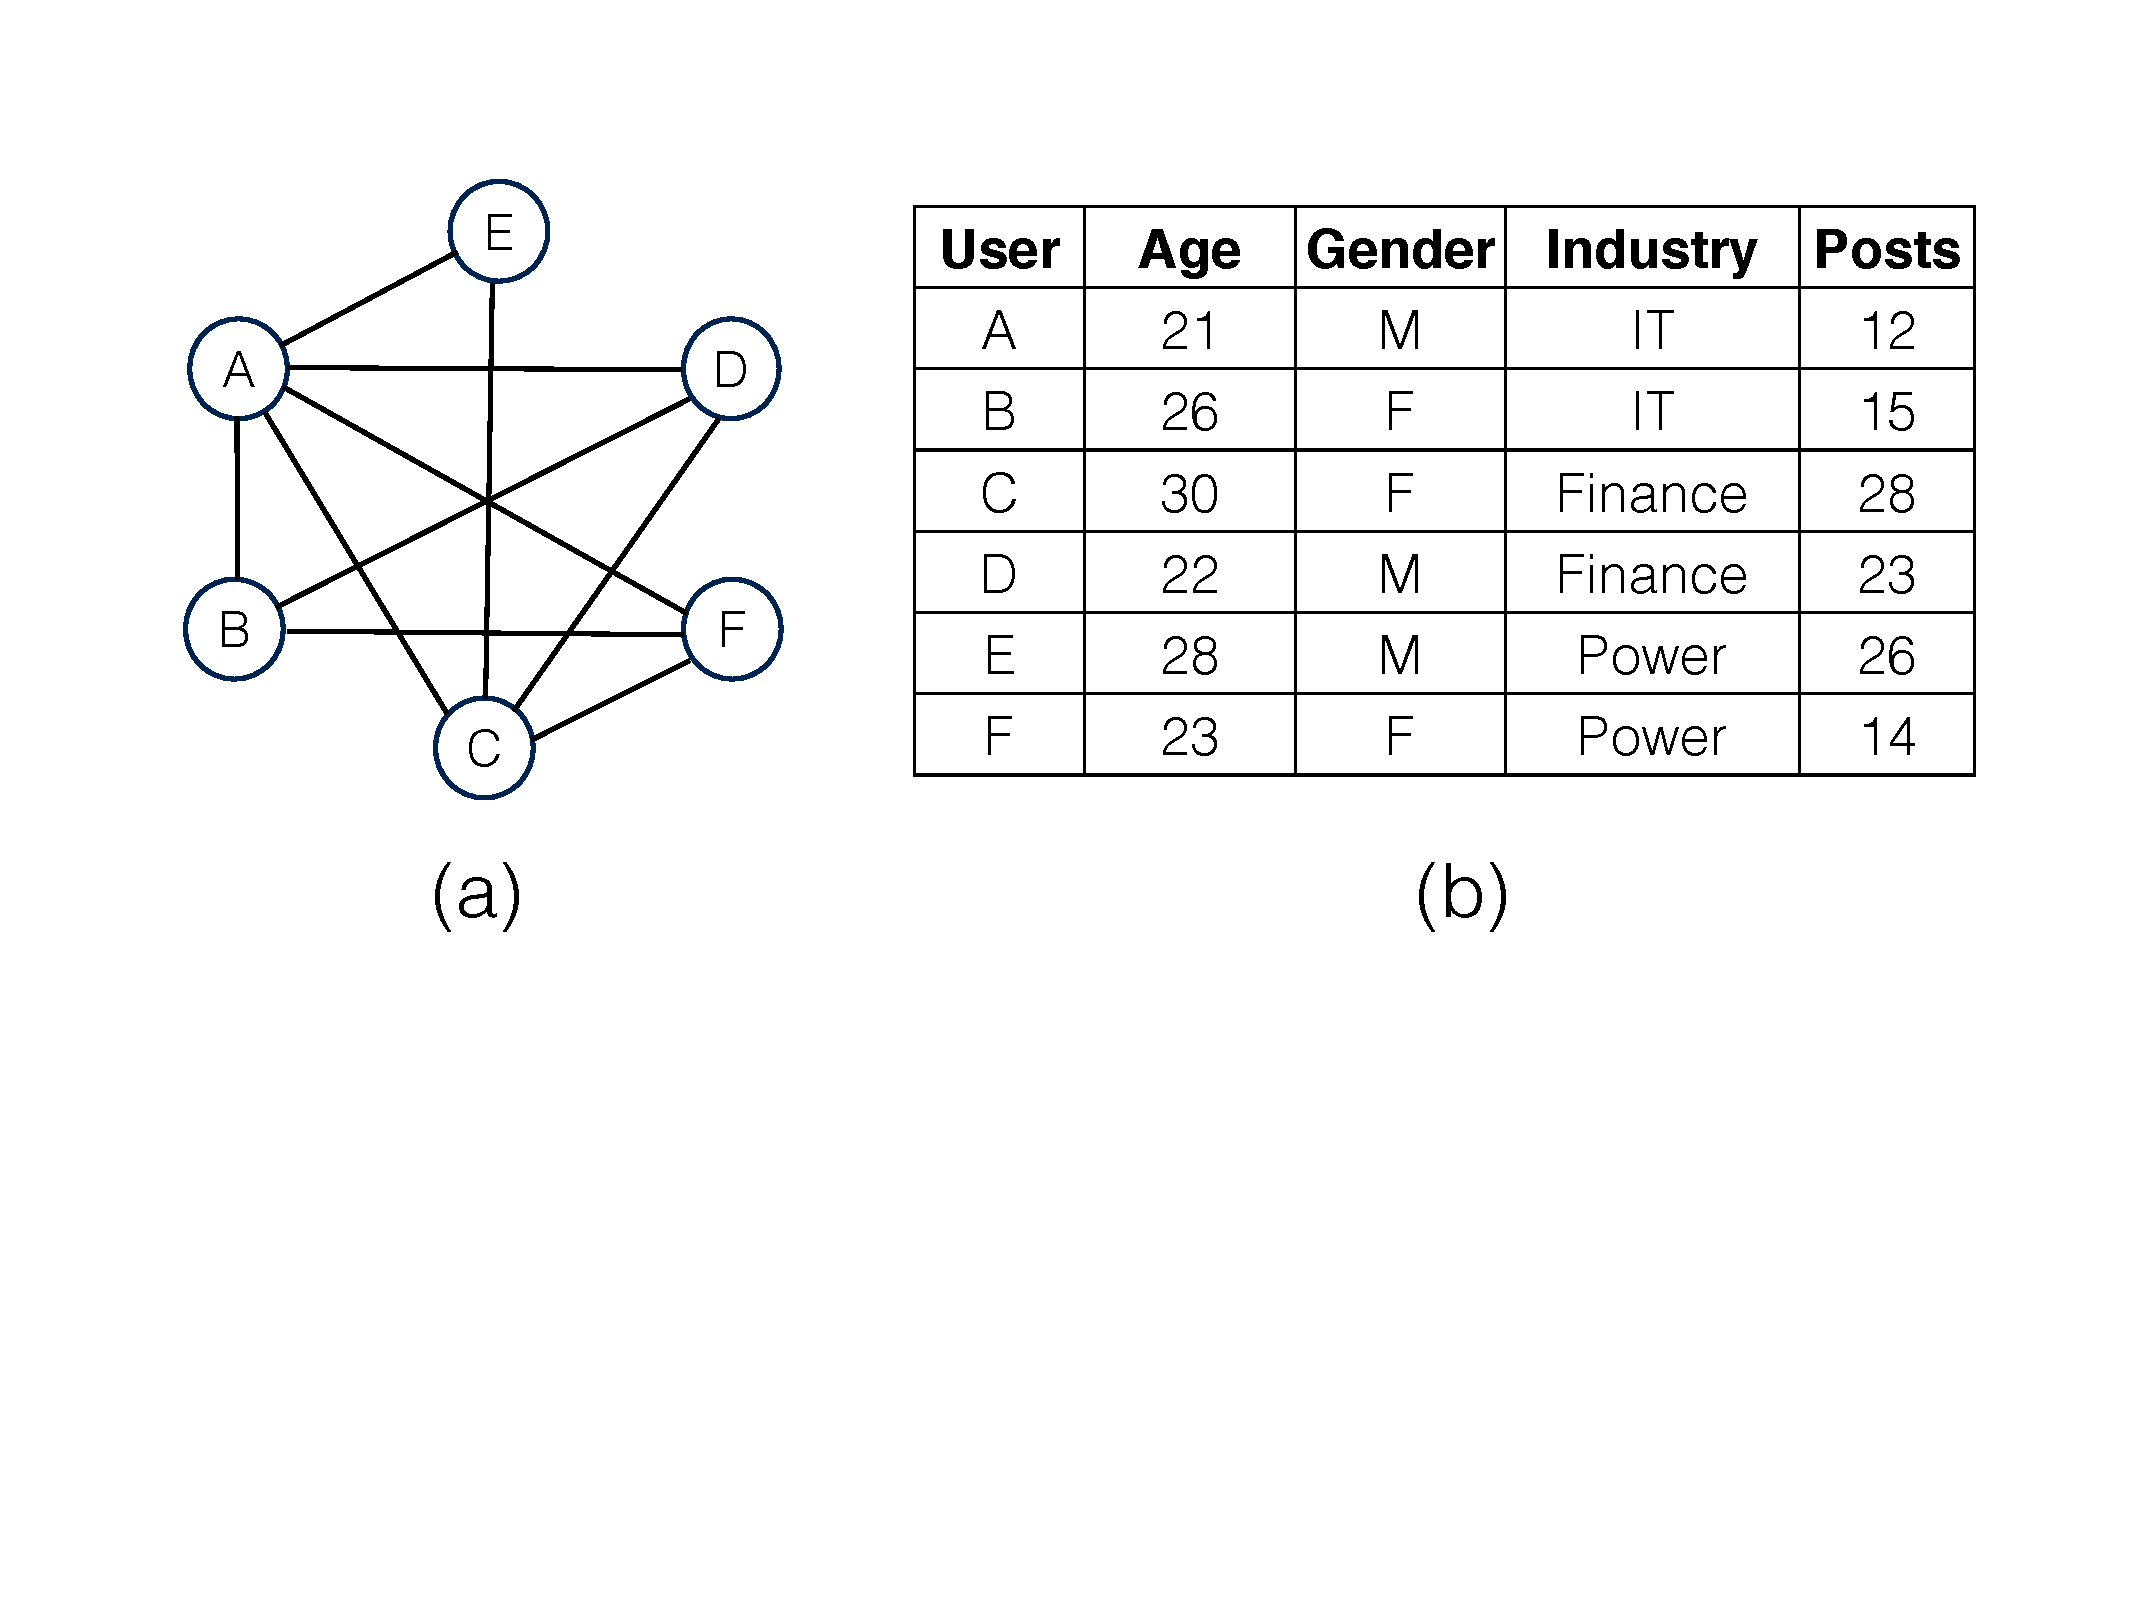
\includegraphics[width=0.8\textwidth]{chapter3/attributed_graph.pdf}
	\caption{A miniature social graph. (a) the graph structure. (b) the attributes associated with the vertexes in (a).} 
	\label{fig:attributed}
\end{figure}

Given a data graph $G = (V,E)$,
a \emph{Graph Window Function (GWF)} over $G$ can be expressed 
as a pair $(W, \Sigma)$, where 
$W(v)$ denotes a \emph{window specification} for a vertex $v \in V$ 
that determines the set of $v$'s neighborhood nodes\footnote{We use ``vertex'' to refer the vertex in the original graph and ``node'' to refer to the vertex in the windows.},
$\Sigma$ denotes an \emph{aggregate function}\footnote{An aggregate function is associated with an attribute. I.e., $\mathtt{average}$(age) and $\mathtt{average}$(salary) are considered to be two different aggregate functions.}.
%, and $A$ denotes  a \emph{vertex attribute}.
The evaluation of a GWF $(W, \Sigma)$ on $G$
computes for each vertex $v$ in $G$, the aggregation $\Sigma$ 
%on the  values of attribute $A$  
over all the nodes in $W(v)$, which is denoted by $\Sigma_{v' \in W(v)} v'$.
%
In this chapter, we focus on the distributive or algebraic aggregate functions (e.g., sum, count, average), as these aggregate functions are widely used in practice. 
%In other words, $W(v)$ refers to a set of vertexes, and the aggregation function 
%$\Sigma$ operates on the values of attribute $A$ over all the vertexes in $W(v)$. 
%Meanwhile, the aggregate function $\Sigma$ is distributive or algebraic (e.g., sum, count, average), as these aggregate functions are widely used in practice. 
 
In the following, we introduce two useful types of window specification (i.e., $W$), namely, 
\emph{k-hop window} and \emph{topological window}.


\begin{definition}[$k$-hop Window] 
Given a vertex $v$ in a data graph $G$, 
the $k$-hop window of $v$, denoted by $W_{kh}(v)$ (or $W(v)$ when there is no ambiguity),
is the set of nodes in $G$ which can be reached by $v$ within $k$ hops.
For an undirected graph $G$,
a node $u$ is in $W_{kh}(v)$  if there is a $\alpha$-hop path between $u$ and $v$ where $\alpha \leqslant k$.
For a directed graph $G$,
a node $u$ is in $W_{kh}(v)$  if there is a $\alpha$-hop directed path from $v$ to $u$\footnote{
Other variants of k-hop window for directed graphs are possible; e.g.,
a node $u$ is in $W_{kh}(v)$  if there is a $\alpha$-hop directed path from $u$ to $v$ where $\alpha \leqslant k$.
} where $\alpha \leqslant k$.
\end{definition}

Intuitively, a $k$-hop window selects the neighboring nodes within a $k$-hop distance. 
These neighboring nodes typically represent the most important 
entities to a vertex with regard to their structural relationship in a graph. 
Thus, the $k$-hop window provides a meaningful specification for many applications, such as customer behavior analysis \cite{briscoe2013determining,dai2012predicting} , digital marketing \cite{ma2010ego} etc.
%\remark{Cite some papers here to justify.}

As an example, in Figure~\ref{fig:attributed}, the $1$-hop window of vertex \emph{E} is $\{A,C,E\}$ and the $2$-hop window of vertex \emph{E} is $\{A,B,C,D,E,F\}$.  

\begin{definition}[Topological Window] 
Given a vertex $v$ in a DAG $G$, the topological window of $v$, denoted by $W_t(v)$,
refers to the set of ancestor nodes of $v$ in $G$,
i.e., a vertex $u$ is in $W_t(v)$ if there is directed path from $u$ to $v$ in $G$.
\end{definition}

There are many directed acyclic graphs (DAGs) in real world applications (such as biological networks, citation networks and dependency networks)
where topological windows represent meaningful relationships that are of interest.
For example, in a citation network where (X,Y) is an edge if paper $X$ cites paper $Y$, 
the topological window of a paper represents the citation impact of that paper \cite{campanario2011empirical,holsapple2003citation,ma2008bringing}.

To illustrate, Figure~\ref{fig:topological} shows a small example of a Pathway Graph from a biological network. 
The topological window of $E$ (i.e., $W_t(E)$) is $\{A, B, C, D, E\}$ and $W_t(H)$ is $\{A, B, D, H\}$.


\begin{figure}[h]
\centering
 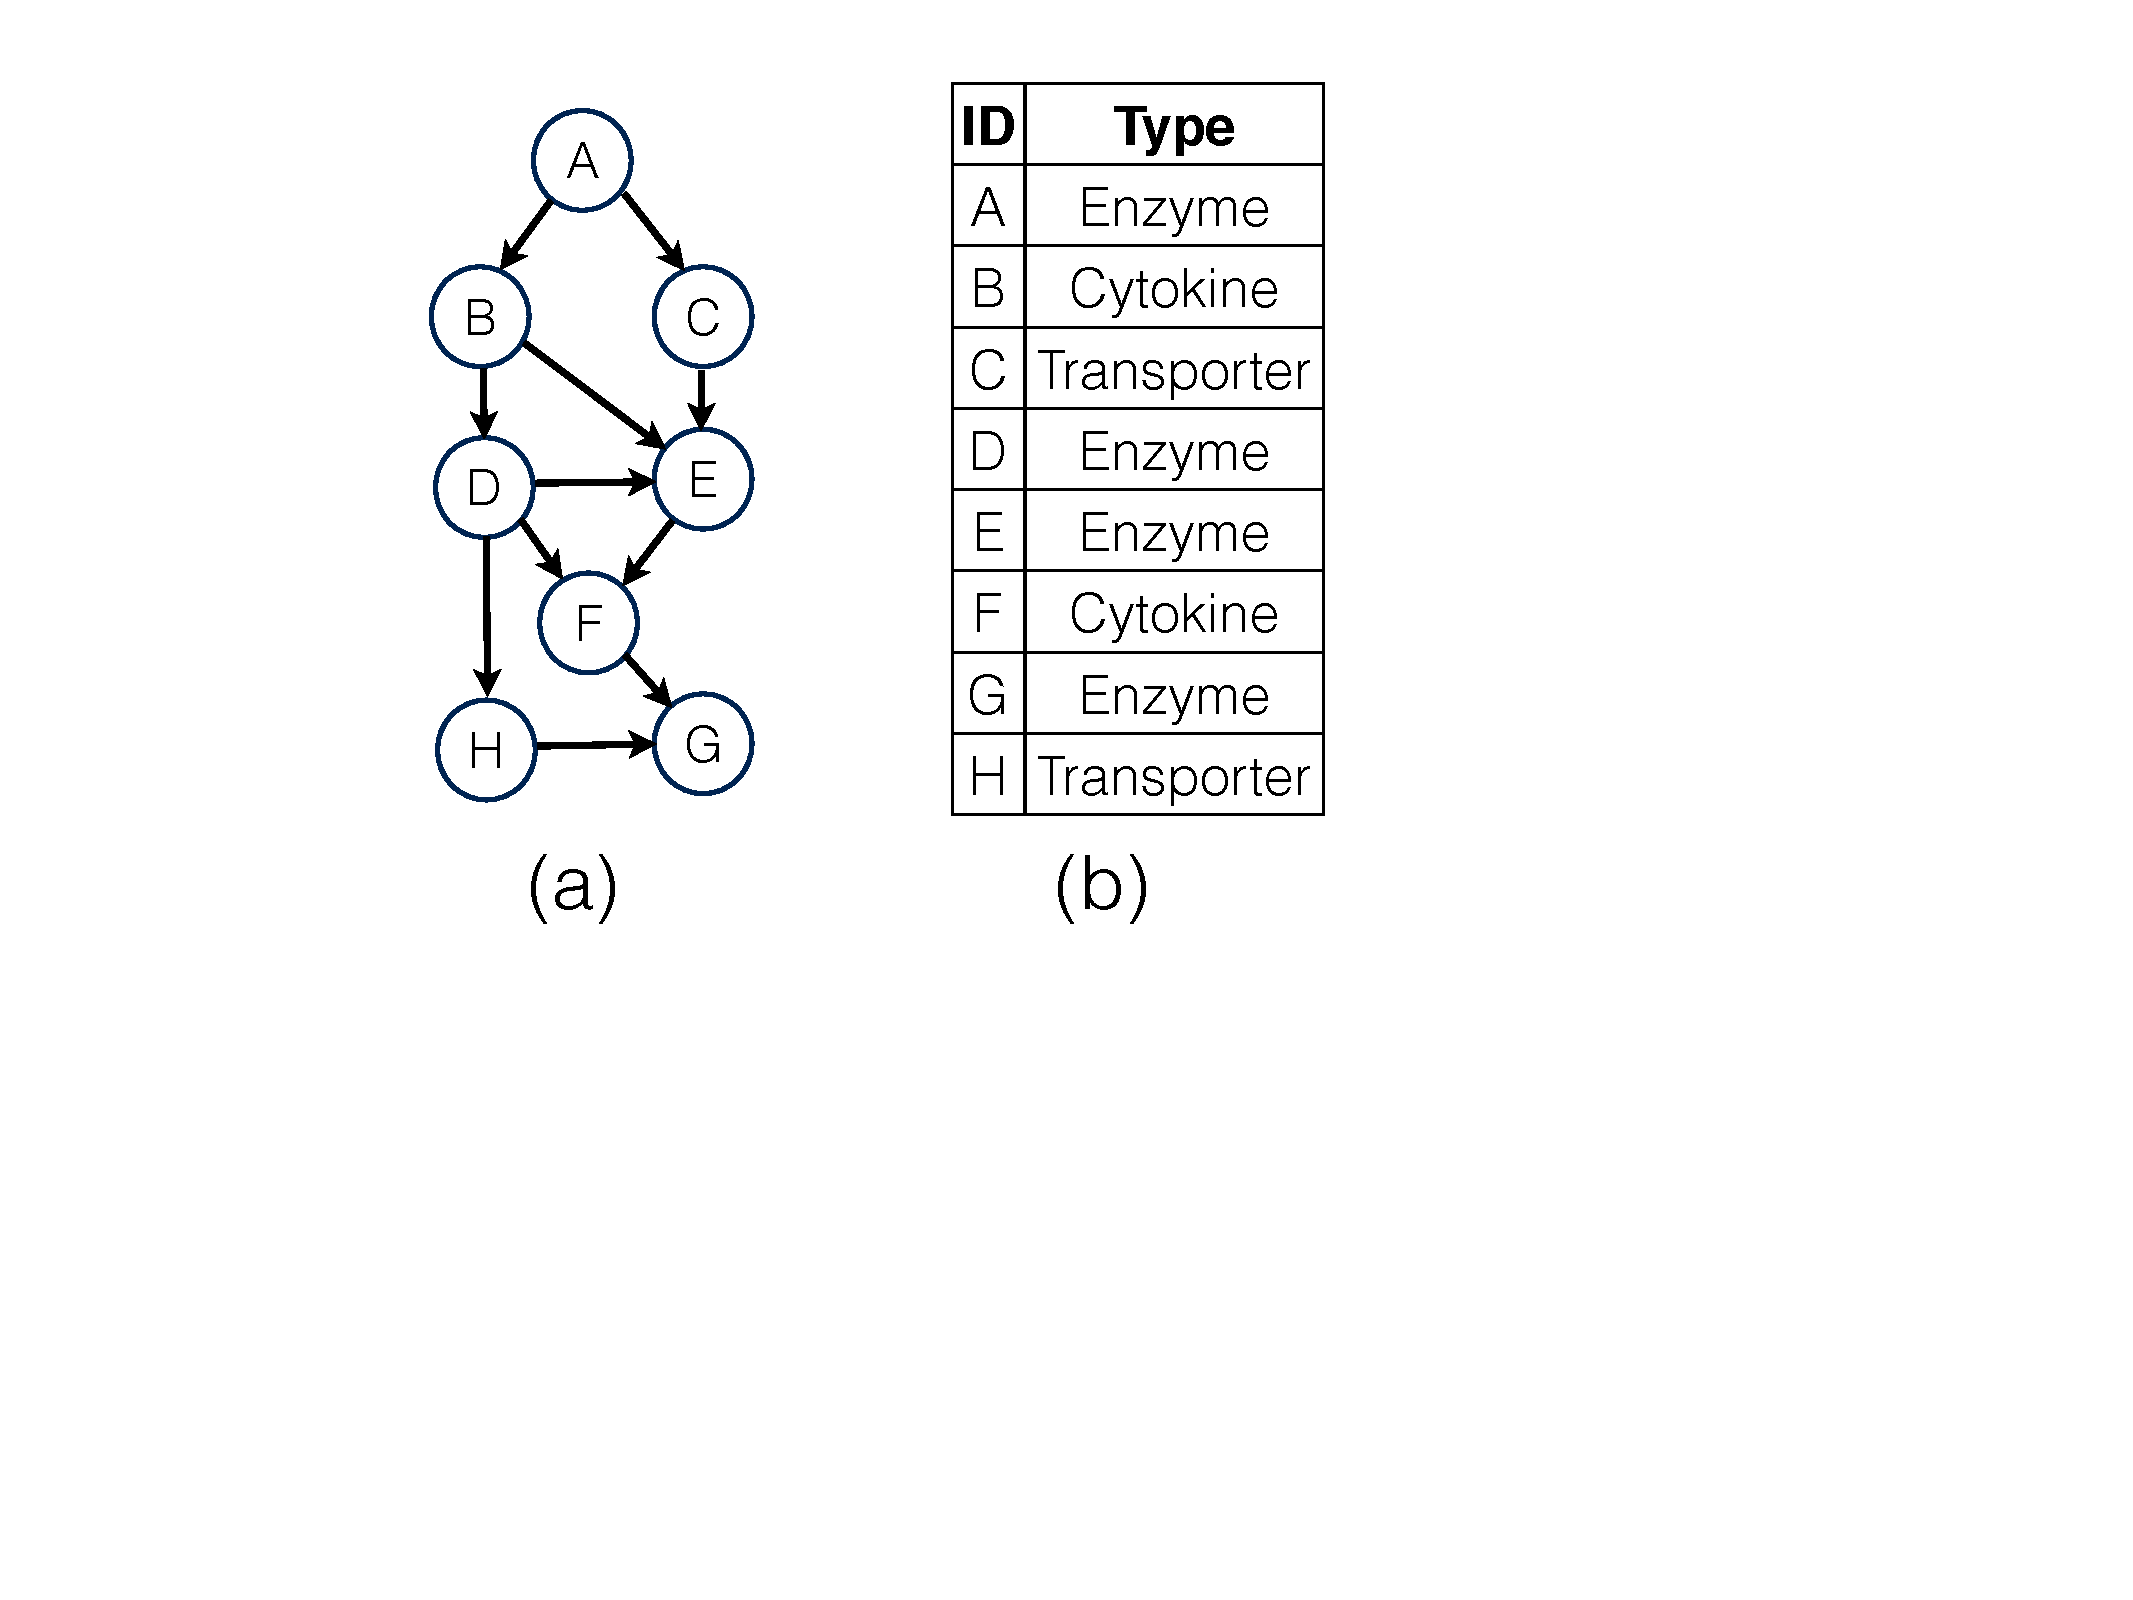
\includegraphics[width=0.8\textwidth]{chapter3/dag.pdf}
	\caption{A miniature pathway DAG. (a) the DAG structure. (b) the attributes associated with the vertexes of (a).}
	\label{fig:topological}
\end{figure}

\begin{definition}[Graph Window Query] 
A graph window query on a data graph $G$ is of the form
$GWQ(G, W_1, \Sigma_1,\cdots, W_m, \Sigma_m)$, where $m \geq 1$
and
each pair $(W_i,\Sigma_i)$ is a graph window function on $G$.
\end{definition}
In this chapter, we focus on graph window queries with a single window 
function that is either a $k$-hop or topological window. 
The evaluation of complex graph window queries with multiple window 
functions can be simply processed as a sequence of window functions one
after another. 
We leave the optimization of processing multiple window functions for future studies.


%
\newcommand{\DBIndex}{DBIndex}
\newcommand{\blockset}{{\cal B}}
\newcommand{\clusterset}{{\cal C}}

\section{Dense Block Index}
A straightforward approach to process a graph window query 
$Q = (G, W, \Sigma, A)$, where $G = (V,E)$,
is to dynamically compute the window $W(v)$ for each vertex $v \in V$ and
its aggregation 
$\Sigma_{v' \in W(v)} v'.A$ 
independently from other vertexes. We refer to this approach as \emph{Non-Indexed} method.

Given that many of the windows would share many common nodes (e.g., the k-hop windows of two adjacent nodes),
such a simple approach would be very inefficient due to the lack of sharing of the aggregation computations. 

To efficiently evaluate graph window queries, we propose an indexing technique named \emph{dense block index} (\textit{\DBIndex}), which is both space and query efficient. 
The main idea of \DBIndex\ is to try to reduce the aggregation computation cost by identifying subsets of nodes that are shared by more than one window 
so that the aggregation for the shared nodes could be computed only once instead of multiple times.

For example, consider a graph window query on the social graph in Fig.~\ref{fig:attributed} using the 1-hop window function.
We have $W(B) = \{A,B,D,F\}$ and $W(C) = \{A,C,D,E,F\}$ sharing three common nodes $A$, $D$, and $F$.
By identifying the set of common nodes $S=\{A,D,F\}$, its aggregation 
$\Sigma_{v \in S} v.A$ can be computed only once
and then reuse to compute the aggregation for $\Sigma_{v \in W(B)} v.A$ and $\Sigma_{v \in W(C)} v.A$.

%Given a graph window query $Q = (G, W, \Sigma, A)$ on a graph $G=(V,E)$,
Given a window function $W$ and a graph $G=(V,E)$,
we refer to a non-empty subset $B \subseteq V$ as a {\it block}.
Moreover, if $B$ contains at least two nodes and $B$ is contained by at least two different windows
(i.e., there exists $v_1, v_2 \in V$, $v_1 \neq v_2$, $B \subseteq W(v_1)$, and $B \subseteq W(v_2)$),
then $B$ is referred to as a {\it dense block}.
Thus, in the last example, $\{A,D,F\}$ is a dense block.

We say that a window $W(X)$ is {\it covered} by a collection of disjoint blocks $\{B_1,\cdots,B_n\}$
if the set of nodes in the window $W(X)$ is equal to the union of all nodes in the collection of disjoint blocks;
i.e., $W(X) = \bigcup_{i=1}^{n} B_i$ and $B_i \cap B_j = \emptyset$ if $i \neq j$.

To maximize the sharing of aggregation computations for a graph window query, 
the objective of \DBIndex\ is to identify a small set of blocks $\blockset$ such that
for each $v \in V$, $W(v)$ is covered by a small subset of disjoint blocks in $\blockset$.
Clearly, the cardinality of $\blockset$ is minimized if $\blockset$ contains a few large dense blocks.

Thus, given a window function $W$ and a graph $G=(V,E)$,
%given a graph window query $Q = (G, W, \Sigma, A)$ on a graph $G=(V,E)$,
a \DBIndex\ to evaluate $W$ on $G$ consists of three components in the form of a bipartite graph.
The first component is a collection of nodes (i.e., $V$);
%The first component is a collection of windows; i.e., $\{W(v) |\ v \in V\}$;
the second component is a collection of blocks; i.e., $\blockset = \{B_1,\cdots,B_n\}$ where each $B_i \subseteq V$;
and the third component is a collection of links from blocks to nodes
such that if a set of blocks $B(v) \subseteq \blockset$ is linked to a node $v \in V$,
then $W(v)$ is covered by $B(v)$.
Note that a \DBIndex\ is independent of both the aggregation function (i.e., $\Sigma$) and the attribute to be aggregated (i.e., $A$).

Fig.~\ref{fig:dbi_agg}(a) shows an example of a \DBIndex\ wrt the social graph in Fig.~\ref{fig:attributed} and the 1-hop window function.
Note that the index consists of a total of seven blocks of which three of them are dense blocks.

\begin{figure}[t]
\centerline{
	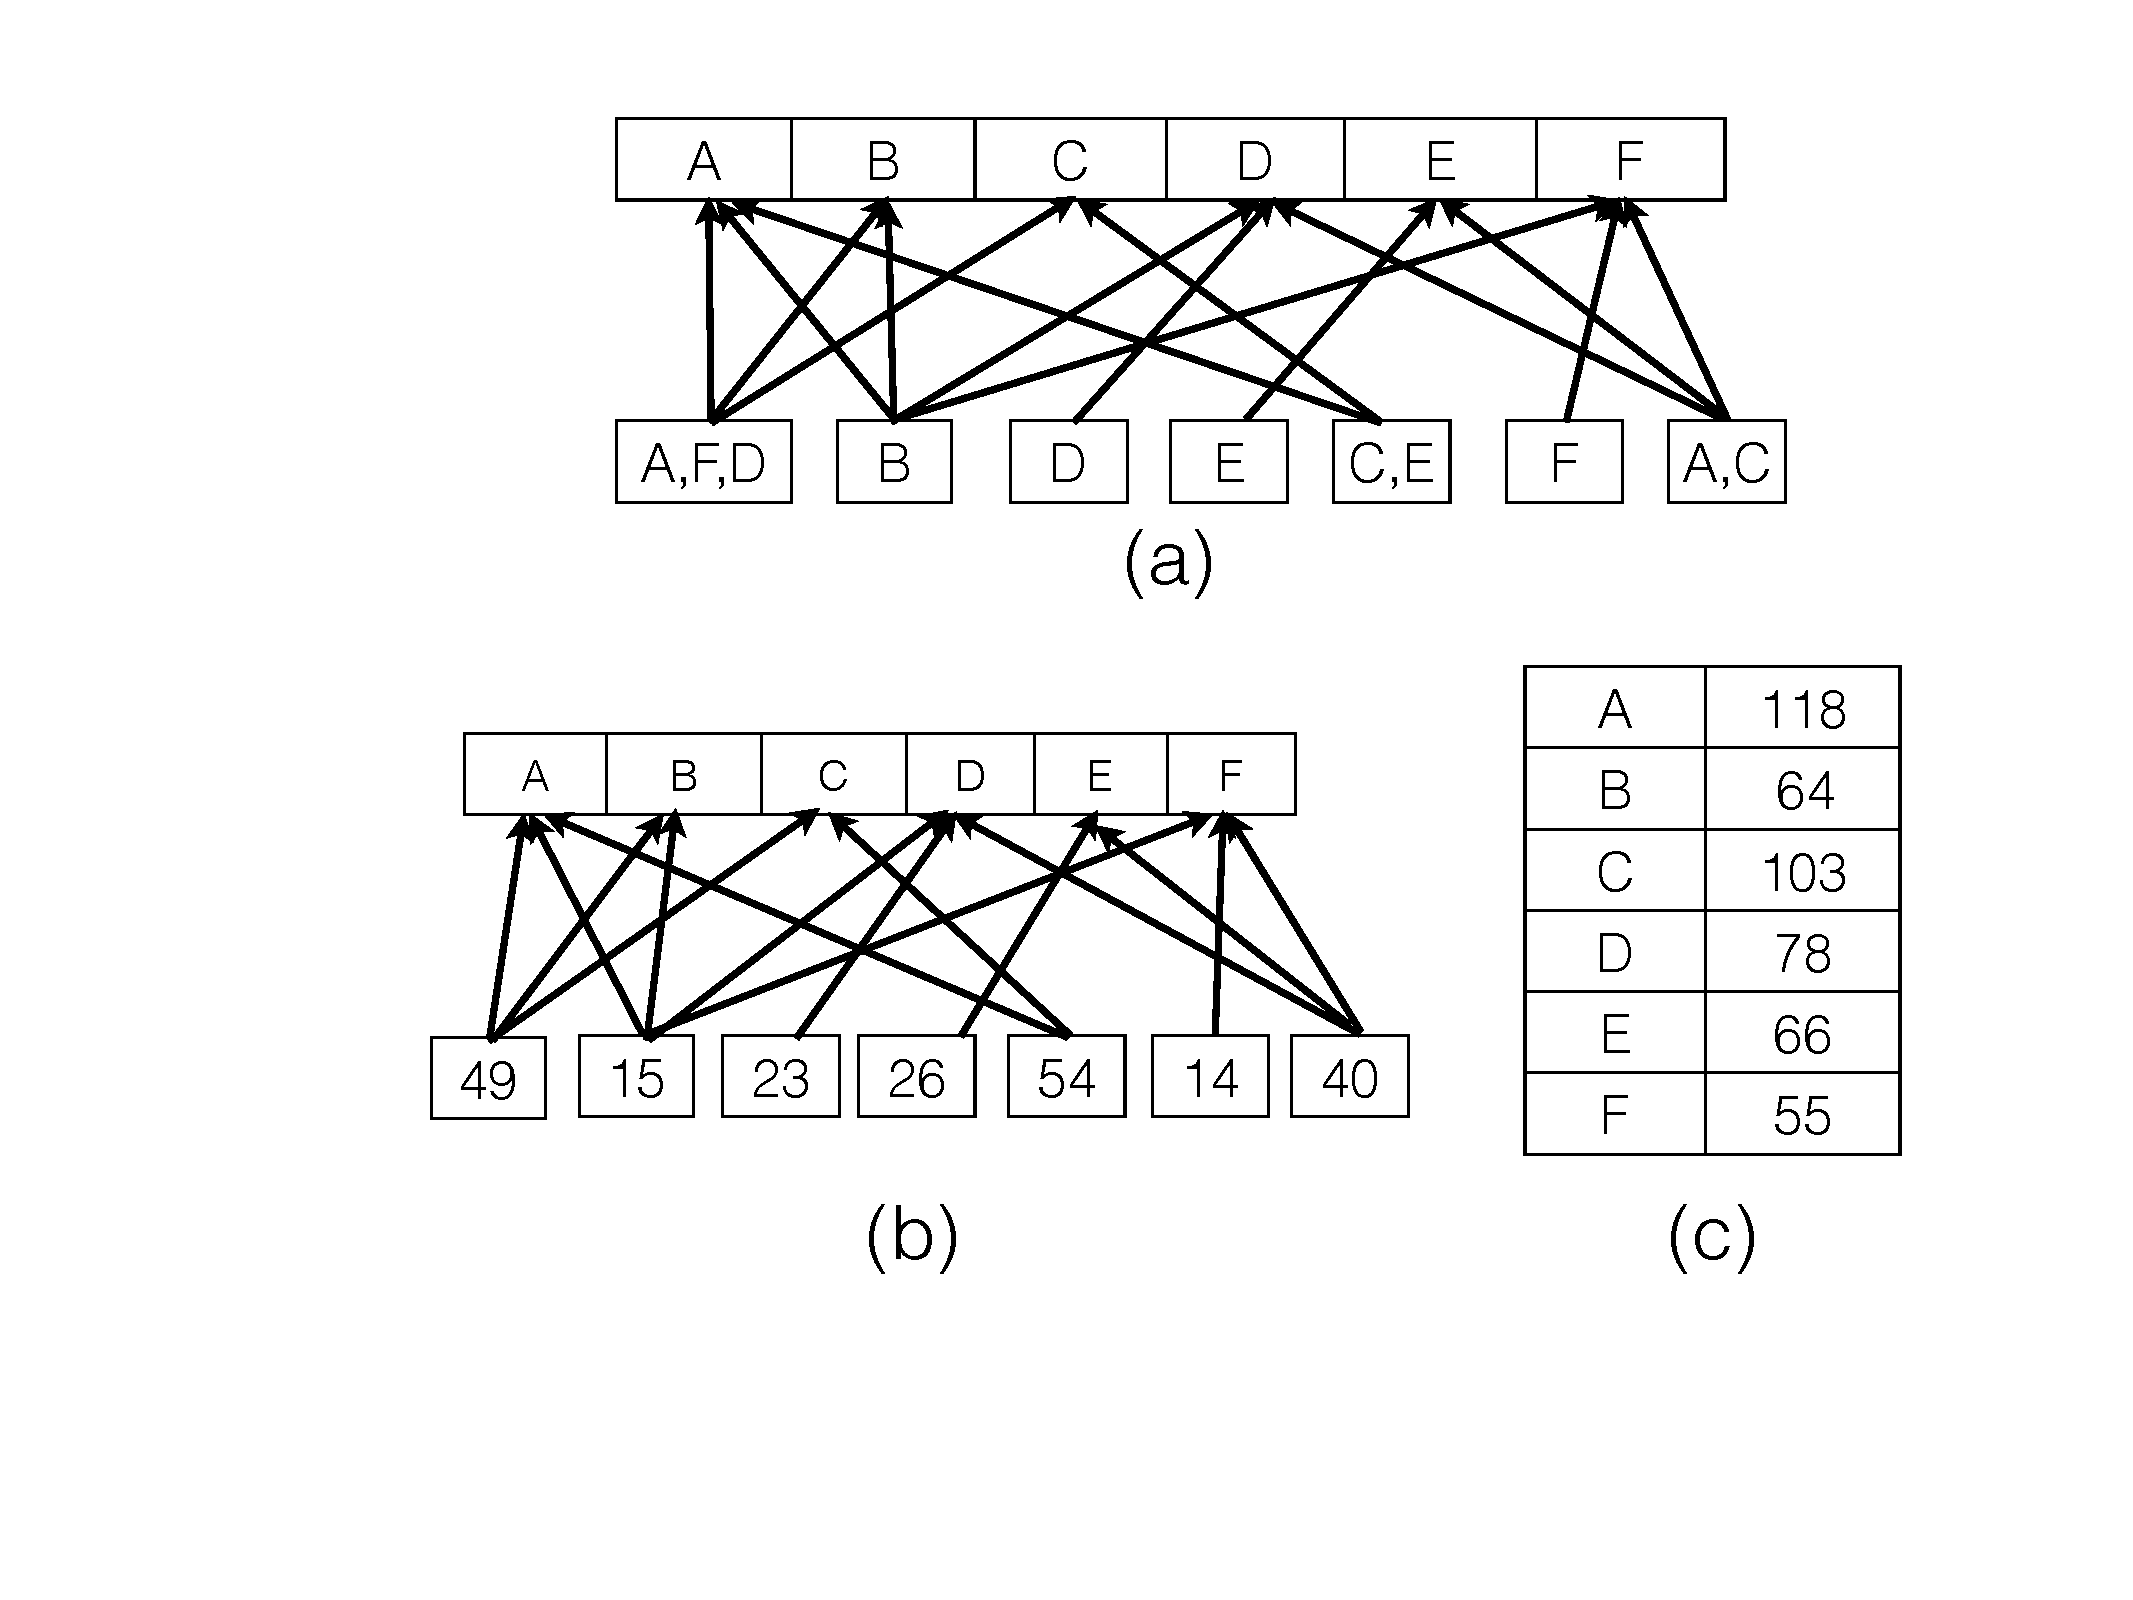
\includegraphics[width=0.8\textwidth]{chapter3/dbi_process} 
	}
	\caption{Window Query Processing using DBIndex. (a) provides the DBIndex for 1-hop window query in Fig.~\ref{fig:attributed}; (b) shows the partial aggregate results based on the dense block; (c) provides the final aggregate value of each window. }
	\label{fig:dbi_agg}
\end{figure}

\subsection{Query Processing using \DBIndex}
Given a \DBIndex\ wrt a graph $G$ and a window function $W$, a graph window query $Q = (G, W, \Sigma, A)$ is processed by the following two steps.
First, for each block $B_i$ in the index, we compute the aggregation (denoted by $T_i$) over all the nodes in $B_i$;
i.e., $T_i = \Sigma_{v \in B_i} v.A$. 
Thus, each $T_i$ is a partial aggregate value.
Next, for each window $W(v)$, $v \in V$, the aggregation for the window is computed by aggregating over all the partial aggregates
associated with the blocks linked to $W(v)$;
i.e., if $B(v)$ is the collection of blocks linked to $W(v)$, 
then the aggregation for $W(v)$ is given by $\Sigma_{B_i \in B(v)} T_i$. 

Consider again the \DBIndex\ shown in Fig.~\ref{fig:dbi_agg}(a) 
defined wrt the social graph in Fig.~\ref{fig:attributed} and the 1-hop window function.
Fig.~\ref{fig:dbi_agg}(b) shows how the index is used to evaluate the graph window query $(G, W, sum, Posts)$
where each block is labeled with its partial aggregate value;
and
Fig.~\ref{fig:dbi_agg}(c) shows the final query results.




%%%%%%%%%%%%%%%%%%%%%%%%%%%%%%%%%%%%%%%%%%%%%%%%%%%%%%%%%%%%%%%%%%%%%%%%%%%%%%%
%%%%%%%%%%%%%%%%%%%%%%%%%%%%%%%%%%%%%%%%%%%%%%%%%%%%%%%%%%%%%%%%%%%%%%%%%%%%%%%
%%%%%%%%%%%%%%%%%%%%%%%%%%%%%%%%%%%%%%%%%%%%%%%%%%%%%%%%%%%%%%%%%%%%%%%%%%%%%%%
%%%%%%%%%%%%%%%%%%%%%%%%%%%%%%%%%%%%%%%%%%%%%%%%%%%%%%%%%%%%%%%%%%%%%%%%%%%%%%%
%%%%%%%%%%%%%%%%%%%%%%%%%%%%%%%%%%%%%%%%%%%%%%%%%%%%%%%%%%%%%%%%%%%%%%%%%%%%%%%

%%%%%%%%%%%%%%%%%%%%%%%%%%%%%%%%%%%%%%%%%%%%%%%%%%%%%%%%%%%%%%%%%%%%
\subsection{\DBIndex\ Construction} 

In this section, we discuss the construction of the \DBIndex\ (wrt a graph $G=(V,E)$ and window function $W$) which has two key challenges.

The first challenge is the time complexity of the index construction. 
From our discussion of query processing using DBIndex, we note that the number of aggregation computations is determined by both the number of blocks as well as the number of links in the index; 
the former determines the number of partial aggregates to compute
while the latter determines the number of aggregations of the partial aggregate values.
Thus, to maximize the shared aggregation computations using DBIndex, both the number of blocks in the index as well as the number of blocks covering each window should be minimized. 
%As discussed, to maximize the shared aggregation computations using \DBIndex,
%both the number of blocks in the index as well as the number of blocks covering each window should be minimized.
However, finding the optimal \DBIndex\ to minimize this objective is NP-hard\footnote{
Note that a simpler variation of our optimization problem has been proven to be NP-hard \cite{vassilevska2004finding}.}.
Therefore, efficient heuristics are needed to construct the \DBIndex.

The second challenge is the space complexity of the index construction.
In order to identify large dense blocks to optimize for query efficiency,
a straightforward approach  is to first derive the window $W(v)$ for each node $v \in V$ and
then use this derived information to identify large dense blocks.
However, this direct approach incurs a high space complexity of $O(|V|^2)$.
Therefore, a more space-efficient approach is needed in order to scale to handle large graphs.

In this section, we present two heuristic approaches, namely {\it MC} and {\it EMC}, to construct \DBIndex.
The second approach EMC is designed to improve the efficiency of the first approach MC for constructing \DBIndex\
(wrt k-hop window function) by using some approxmation techique at the expense of possibly sacrificing 
the ``quality'' of the dense blocks (in terms of their sizes).

%%%%%%%%%%%%%%%%%%%%%%%%%%%%%%%%%%%%%%%%%%%%%%%%%%%%%%%%%%%%%%%%
\subsubsection{MinHash Clustering (MC)}

To reduce both the time and space complexities for the index construction,
instead of trying to identify large dense blocks among a large collection of windows,
we first partition all the windows 
into a number of smaller clusters of similar windows and then identify large dense blocks for each of the smaller clusters.
Intuitively, two windows are considered to be highly similar if they share a larger subset of nodes.
We apply the well-known {\it MinHash based Clustering (MC)} algorithm \cite{broder1997syntactic} to partition the windows into clusters of similar windows.
The MinHash clustering algorithm is based on using the
\emph{Jaccard Coefficient} to measure the similarity of two sets.  
Given the two window $W(v)$ and $W(u)$, $u,v \in V$,
their \emph{Jaccard Coefficient} is given by
\begin{equation} \label{eq:jacc_sim}
	J(u,v) = \frac{|W(u) \cap W(v)|}{|W(u) \cup W(v)|}
\end{equation}
The \emph{Jaccard Coefficient} ranges from 0 to 1, where  a larger value means that the windows are more similar.

\begin{figure}[htb]
\centering
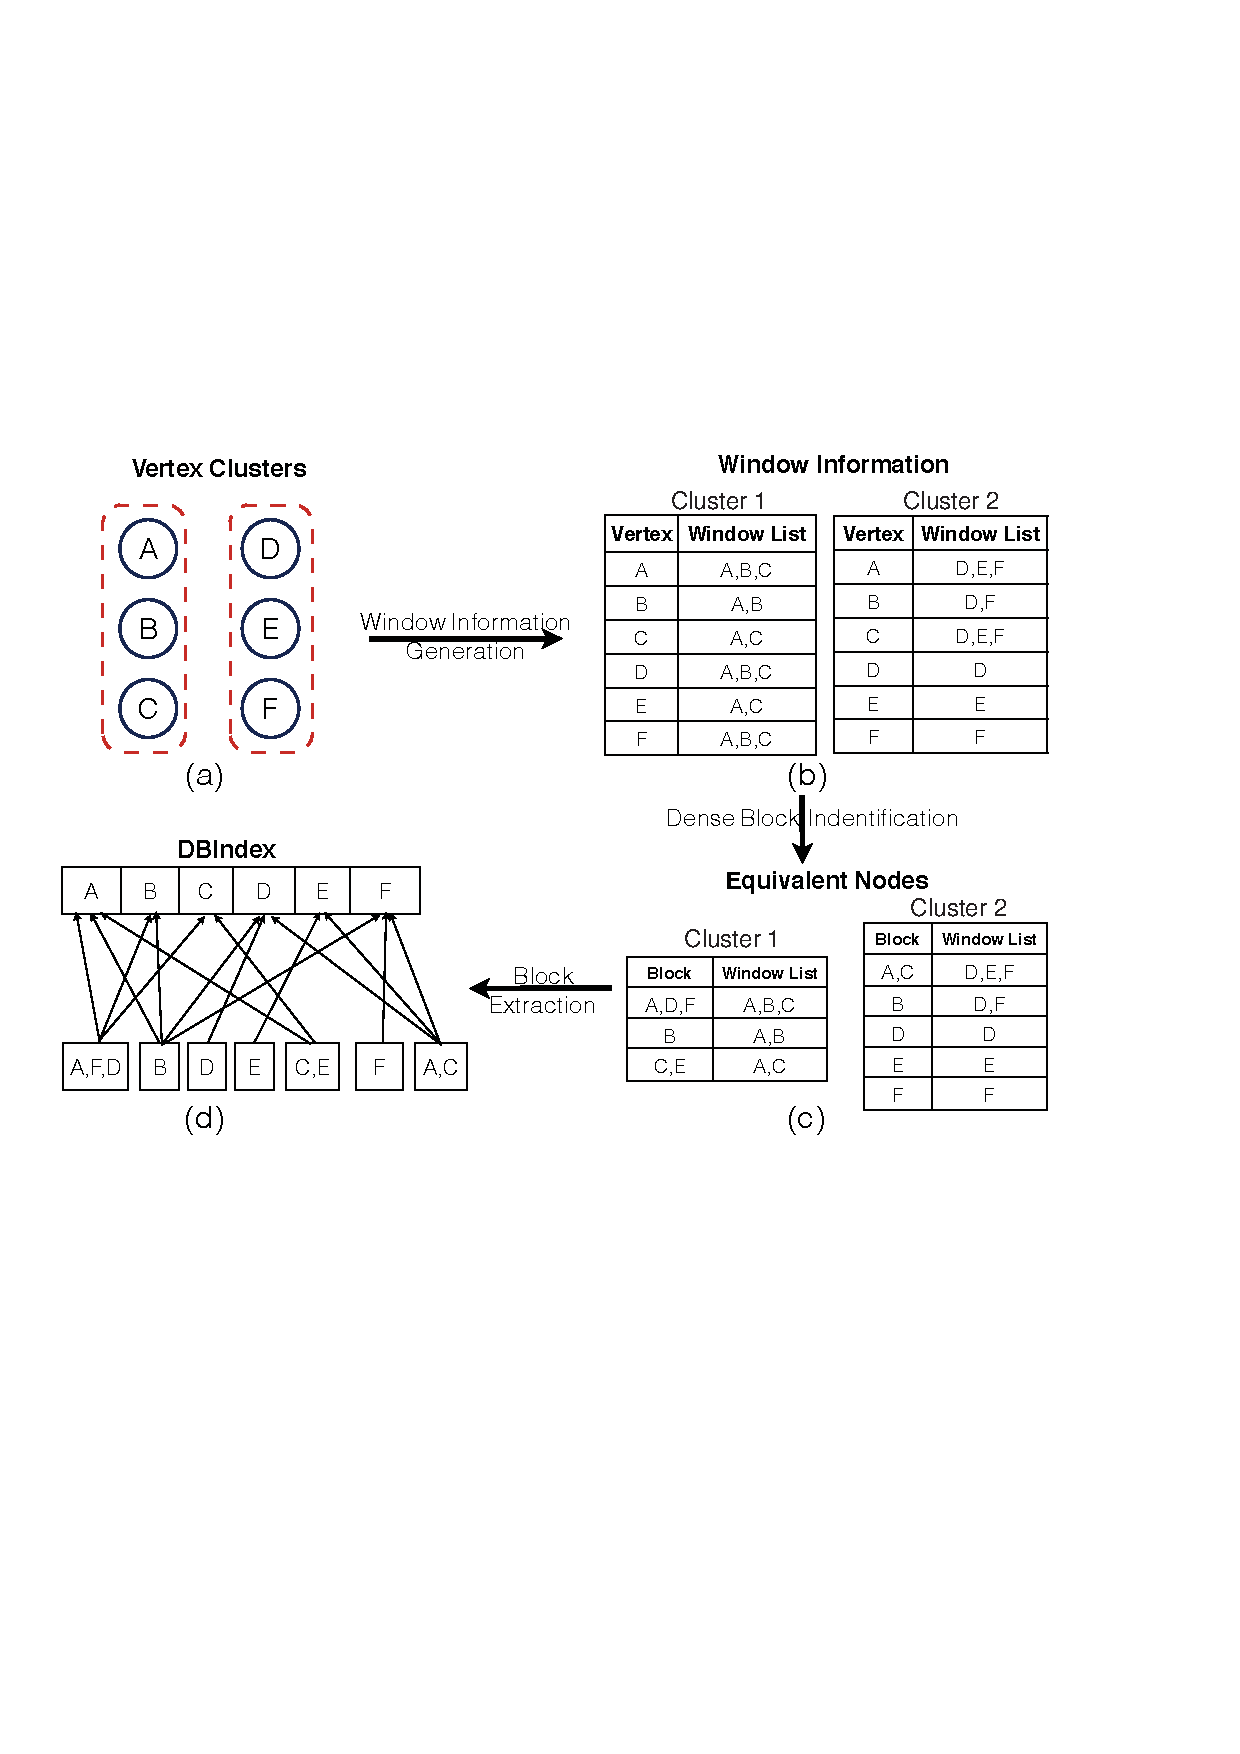
\includegraphics[width=0.8\textwidth]{chapter3/dbi_indexing.pdf}
\caption{DBIndex Construction over Social Graph in Fig.~\ref{fig:attributed}. (a) shows two clusters after MinHash clustering; (b) shows the window information of involved vertices within each cluster; (c) shows the dense blocks within each cluster; (d) provides the final DBIndex.}
\label{fig:dbi-indexing}
\end{figure}


Our heuristic approach to construct \DBIndex\ $I$ operates as follows.
Let $nodes(I)$, $blocks(I)$, and $links(I)$ denote, respectively,
the collection of nodes, blocks, and links that form $I$.
Initially, we have $nodes(I) = V$,
$blocks(I) = \emptyset$,
and
$links(I) = \emptyset$.
\begin{algorithm}
\caption{CreateDBIndex}
\begin{algorithmic}[1]  \small
%\FUNCTION $dbiGen$
\Require Graph $G=(V,E)$, window function $W$
\Ensure \DBIndex\ $I$
\State Initialize \DBIndex\ $I$: $nodes(I)=V$, $blocks(I)=\emptyset$, $links(I)=\emptyset$
\ForAll{$v \in V$}
	\State Traverse $G$ to determine $W(v)$
	\State Compute the hash signature $H(v)$ for $W(v)$
\EndFor
\State Partition $V$ into clusters $\clusterset = \{C_1,C_2,\cdots\}$ based on hash signatures $H(v)$
\ForAll{$C_i \in \clusterset$}
	\ForAll{$v \in C_i$} 
		\State Traverse $G$ to determine $W(v)$
	\EndFor
	\State {\tt IdentifyDenseBlocks} $(I,G,W,C_i)$
\EndFor
\Return $I$
\end{algorithmic}
\label{algo:k-hop-dbi}
\end{algorithm}

The first step is to partition the nodes in $V$ into clusters
using MinHash algorithm such that nodes with similar windows belong to the same cluster. 
For each node $v \in V$, we first derive its window $W(v)$ by an appropriate traversal of the graph $G$.
Next, we compute a hash signature (denoted by $H(v)$) for $W(v)$ based on applying $m$ hash functions on the set $W(v)$.
Nodes with identical hash signatures are considered to have highly similar windows and are grouped into the same cluster.
To ensure that our approach is scalable,
we do not retain $W(v)$ in memory  after its hash signature $H(v)$ has been computed and used to cluster $v$;
i.e., our approach does not materialize all the windows in the memory to avoid high space complexity.
Let $\clusterset = \{C_1,C_2,\cdots\}$ denote the collection of clusters obtained from the first step,
where each $C_i$ is a subset of nodes.
%A cluster is classified as {\it trivial} if it contains only one window; otherwise, it is classified as {\it non-trivial}.

The second step is to identify dense blocks from each of the clusters computed in the first step.
%For each cluster $C_i \in \clusterset$,
%let $N_i$ denote the union of all the nodes in all the windows in $C_i$;
%i.e., $N_i = \{v \in W(u) |\ W(u) \in C_i\}$.
The identification of dense blocks in each cluster $C_i$ is based on the notion of node equivalence defined as follows.
Two distinct nodes $u, v \in C_i$ are defined to be equivalent (denoted by $u \equiv v$)
if $u$ and $v$ are both contained in the same set of windows;
i.e., for every window $W(x), x \in C_i$, $u \in W(x)$ iff $v \in W(x)$.
Based on this notion of node equivalence, $C_i$ is partitioned into blocks of equivalent nodes.
To perform this partitioning, we need to again traverse the graph for each node $v \in C_i$ to 
determine its window $W(v)$\footnote{
Note that although we could have avoided deriving $W(v)$ a second time if we had materialzed all the derived windows the first time, our approach is designed to avoid the space complexity of materializing all the windows in memory at the cost of computing each $W(v)$ twice. We present an optimization in Section~\ref{sec:optimized} to avoid the recomputation cost.
}.
%However, since $C_i$ is now  a smaller cluster of nodes, we can now materialize all the windows for the nodes in $C_i$ in memory without exceeding the memory space.

However, since $C_i$ is now a smaller cluster of nodes, we can now materialize all the windows for the nodes in $C_i$ in memory without exceeding the memory space. In the event that a cluster $C_i$ is still too large for all its vertex windows to be materialized in main memory, we can further partition $C_i$ into equal size sub-clusters. This re-partition process can be recursively performed until the sub clusters created are small enough such that the windows for all nodes in the sub clusters fit in memory. 


Recall that a block $B$ is a dense block if $B$ contains at least two nodes and
$B$ is contained in at least two windows.
Thus, we can classify the nodes in each $C_i$ as either dense or non-dense nodes:
a node $v \in C_i$ is classified as a {\it dense node} if $v$ is contained in a dense block;
otherwise, $v$ is a non-dense node.

For each dense block $B$ in $C_i$,
we update the blocks and links in the \DBIndex\ $I$ as follows:
we insert $B$ into $blocks(I)$ if $B \not\in blocks(I)$,
and we insert $(B,v)$ into $links(I)$
for each $v \in C_i$ where $B \subseteq W(v)$.
If all the blocks in $C_i$ are dense blocks, then we are done with identifying dense blocks in $C_i$;
otherwise, there are two cases to consider.
%otherwise, we update $C_i$ by removing all the dense nodes from $C_i$ and recursively apply the
%two-step procedure on the updated $C_i$ to try to identify more dense blocks.
For the first case, if all the nodes in $C_i$ are non-dense nodes,
then we also terminate the process  of identifying dense blocks in $C_i$
and update the blocks and links in the \DBIndex\ $I$ as before:
we insert each non-dense block $B$ into $blocks(I)$,
and we insert $(B,v)$ into $links(I)$ for each $v \in C_i$ where $B \subseteq W(v)$.
For the second case, if $C_i$ has a mixture of dense and non-dense nodes,
we remove the dense nodes from $C_i$ and recursively identify dense blocks in $C_i$
following the above two-step procedure.

Note that since the blocks are identified independently from each cluster,
it might be possible for the same block to be identified from different clusters.
We avoid duplicating the same block in $blocks(I)$ by checking that a block $B$ is not already in $blocks(I)$
before inserting it into $blocks(I)$.
The details of the construction algorithm are shown as Algorithms
\ref{algo:k-hop-dbi},
\ref{algo:identify},
and
\ref{algo:refine}.

%begin{algorithm}
%\caption{IdentifyDenseBlocks}
%\begin{algorithmic}[1]
%\REQUIRE \DBIndex\ $I$, Graph $G=(V,E)$, window function $W$, a cluster $C_i \subseteq V$
%%\ENSURE \DBIndex
%\STATE Partition $C_i$ into blocks based on node equivalence
%\STATE Initialize $DenseNodes = \emptyset$
%\FORALL{dense block $B$}
% \STATE Insert $B$ into $blocks(I)$ if $B \not\in blocks(I)$
% \STATE Insert $(B,v)$ into $links(I)$ for each $v \in C_i$ where $B \subseteq W(v)$
% \STATE $DenseNodes = DenseNodes \cup B$
%\ENDFOR
%\IF{($DenseNodes = \emptyset$)}
% \FORALL{block $B$}
%  \STATE Insert $B$ into $blocks(I)$ if $B \not\in blocks(I)$
%  \STATE Insert $(B,v)$ into $links(I)$ for each $v \in C_i$ where $B \subseteq W(v)$
% \ENDFOR
%\ELSIF{($C_i - DenseNodes \neq \emptyset$)}
% \IF{($C_i \neq DenseNodes$)}
%  \STATE {\tt RefineCluster} $(I,G,W,C_i - DenseNodes)$
%  \ENDIF
%\ENDIF
%\end{algorithmic}
%\label{algo:identify}
%\end{algorithm}

\begin{algorithm}
\caption{IdentifyDenseBlocks}
\begin{algorithmic}[1] \small
\Require \DBIndex\ $I$, Graph $G=(V,E)$, window function $W$, a cluster $C_i \subseteq V$
%\ENSURE \DBIndex
\State Partition $C_i$ into blocks based on node equivalence
\State Initialize $DenseNodes = \emptyset$
\ForAll{dense block $B$}
	\State Insert $B$ into $blocks(I)$ if $B \not\in blocks(I)$
	\State Insert $(B,v)$ into $links(I)$ for each $v \in C_i$ where $B \subseteq W(v)$
	\State $DenseNodes = DenseNodes \cup B$
\EndFor
\If{($DenseNodes = \emptyset$)}
	\ForAll{block $B$}
		\State Insert $B$ into $blocks(I)$ if $B \not\in blocks(I)$
		\State Insert $(B,v)$ into $links(I)$ for each $v \in C_i$ where $B \subseteq W(v)$
	\EndFor
\ElsIf{($C_i - DenseNodes \neq \emptyset$)}
	\If{($C_i \neq DenseNodes$)}
		\State {\tt RefineCluster} $(I,G,W,C_i - DenseNodes)$
	\EndIf
\EndIf
\end{algorithmic}
\label{algo:identify}
\end{algorithm}

Figure~\ref{fig:dbi-indexing} 
illustrates the construction of the DBIndex with respect to the social graph in 
Figure~\ref{fig:attributed}(a) and 1-hop window using the MC algorithm.
First, the set of graph vertexes are partitioned into clusters using MinHash clustering;
Figure~\ref{fig:dbi-indexing}(a)
shows that the set of vertexes $V = \{A, B, C, D, E, F \}$ are partitioned into two clusters $C_1=\{A, B, C\}$ and $C_2=\{D, E, F\}$. 

For convenience, cluster 1 in 
Figure~\ref{fig:dbi-indexing}(b) shows for each $v \in C_1$, the set of vertexes whose windows contain $v$;
i.e., $\{u |\ v \in W(u)\}$.
Similarly, Cluster 2 in Fig.~\ref{fig:dbi-indexing} (b)
shows for each $v \in C_2$, the set of vertexes whose windows contain $v$.
Consider the identification of dense blocks in cluster $C_1$.
As shown in Figure~\ref{fig:dbi-indexing} (c), based on the notion of equivalence nodes,
cluster $C_1$ is partitioned into three blocks of equivalent nodes:
$B_1=\{A,D,F\}$, $B_2=\{B\}$, and $B_3\{C,E\}$.
Among these three blocks, only
$B_1$ and $B_3$ are dense blocks.
The MC algorithm then tries to repartition the window $A,B,C$ using non-dense nodes in $C_1$,
(i.e., $B_2$). Since $B_2$ is the only non-dense node, it directly outputs.
%the remaining non-dense nodes in $C_1$ (i.e., $\{B\}$).
At the end of processing cluster $C_1$,
the DBIndex $I$ is updated as follows:
$blocks(I) = \{B_1, B_2, B_3\}$ 
and
$links(I) = \{ (B_1,\{A,B,C\}), (B_2, \{A,B\}),$, $(B_3, \{A,C\}) \}$. The identification of dense blocks in cluster $C_2$ 
is of similar process.

We find it is non-trivial to precisely analyze the complexity of Algorithm~\ref{algo:k-hop-dbi}. Here, we only offer a brief analysis. Suppose the MinHash cost is $H$ and the total cost for k-bounded BFS for all vertex is $B$, Lines 1-5 has the complexity of $O(H + B)$.  Lines 7-10 has the complexity of $O(B)$. A single execution of Algorithm~\ref{algo:identify}  has the  complexity of $O(|V|)$, since we can simply partition nodes using hashing. Suppose the iteration runs for $K$ times, the total cost for Algorithm~\ref{algo:identify} and Algorithm~\ref{algo:refine} is $O(K|V|)$. Therefore the overall complexity of Algorithm~\ref{algo:k-hop-dbi} is $O(H+2*B + O(K|V|))$. $H$ depends on the number of vertex-window mappings for a given query and $B$ depends on the graph structure and number of hops. As we demonstrate in Section 6, the $H$ and $B$ are the major contribution of the indexing time. To reduce the index time, we provide further optimization techniques.


\begin{algorithm}
\caption{RefineCluster}
\begin{algorithmic}[1]
\Require \DBIndex\ $I$, Graph $G=(V,E)$, window function $W$, a cluster $C \subseteq V$
%\ENSURE \DBIndex
\ForAll{$v \in C$}
	\State Compute the hash signature $H(v)$ for $W(v) \cap C$
\EndFor
\State Partition $C$ into clusters $\clusterset = \{C_1,C_2,\cdots\}$ based on hash signatures $H(v)$
\ForAll{$C_i \in \clusterset$}
	\State {\tt IdentifyDenseBlocks} $(I,G,W,C_i)$
\EndFor
\end{algorithmic}
\label{algo:refine}
\end{algorithm}

\subsubsection{Estimated MinHash Clustering (EMC)}
\label{sec:optimized}

The MC approach described in the previous section requires the window of each node (i.e., $W(v), v \in V$)
to be computed twice in order to avoid the high space complexity of materializing all the windows in main memory.
For k-hop window function with a large value of $k$, the cost of graph traverals to compute the k-hop windows
could incur a high computation overhead. Moreover, the cost of initial MinHash in MC approach equals to the initial number of vertex-window mappings, which is of the same order as graph traversal. For the larger hops, MinHash clustering would incur high computation cost.

To address these issues, we present an even more efficient approach,
referred to as {\it Estimated MinHash Clustering (EMC)}, 
to optimize the construction of the \DBIndex\ for k-hop window function with larger k.

The key idea behind $EMC$ is based on the observation that for any two nodes $u, v \in V$,
if their $m$-hop windows, $W_m(u)$ and $W_m(v)$, are highly similar 
and they are grouped into the same cluster, 
then it is likely that the $n$-hop windows of these two nodes, where $n > m$,
would also be highly similar and grouped into the same cluster.

Using the above observation, we could reduce the overhead cost for constructing a \DBIndex\ wrt a $k$-hop window 
function by clustering the nodes based on their $k'$-hop windows, where $k' < k$, instead of their $k$-hop windows.

To reduce the overhead of window computations,
our $EMC$ approach is similar to the MC approach except   
for the first round of window computations
(line 3 in Algorithm \ref{algo:k-hop-dbi}):
$EMC$ uses lower hop windows to approximate $k$-hop windows for the purpose of clustering the nodes in $V$.
Thus, the hash signatures used for partitioning $V$ are based on lower hop windows.
This approximation clearly has the advantage of improved time-efficiency as traversing and Minhashing on lower hop window is of
order of magnitude faster. For the extreme case, adapting 1-hop window of a node $v$ requires only accessing the adjacent nodes of $v$. 
The tradeoff for this improved efficiency is that the ``quality'' of the dense blocks might be reduced (in terms of their sizes).
However, our experimental results show that this reduction in quality is actually only marginal which makes this approximation a worthy tradeoff.


\subsubsection {Justification of Heuristic}
In the following, we show the theoretical justification of our heuristic: the Jaccard coefficient
is increasing with respect to the number of hops for a large class of graphs. We 
assume that the degree of vertexes follows the same distribution, which is true in most
real-networks and random graph models\footnote{E.g. Social network, Preferential Attachment model etc. follow
power-law distribution. However, our analysis works for other distribution as well.}.  
This implies we can analyze vertexes 
with their neighborhoods structure using a unified way. 

We use $d_i$ to indicate the degree of vertex $i$. For any vertex pair $(u,v)$, their 
intersection on $k$-hop window consists of three part. We name them using $A=W_k(u)-W_k(v)$, 
$B=W_k(v)-W_k(u)$ and $C_k = W_k(u) \cap W_k(v)$. Clearly the Jaccard coefficient at $k$-hops
can be expressed as follows:
\begin{equation}
	J_k(u,v) = \frac{|C_k|}{|A_k| + |B_k| + |C_k|}
\end{equation}

To deduct the relationship between $J_k(u,v)$ and $J_{k+1}(u,v)$, we prove the following lemma first:
\begin{theorem}
Let $S$ be a collection of connected vertexes, the number of newly discovered
vertexes by one-hop expansion from $S$ is bounded by a function on $|S|$.
\end{theorem}
\begin{proof}
Consider a random variable $Y_i$ indicate the newly 
discovered vertexes from one-hop expansion from vertex $i$. 
Then the probability of $|Y_i|=y$ is can be analyzed as follows: there 
are $d_i$ edges for vertex $i$. Since $|Y_i|$ is connected with $S$, one edge
is fixed to link with a vertex in $S$. There are remaining $d_i-1$ edges with
$y$ edges linked to the new vertexes. In total, there are $|V|-1 \choose d_i -1$
combinations with $d_i$ edges. Therefore, the probability can be written as:
\begin{equation}
Prob(Y_i = y| v_i \in S) = \frac{{|S| -1 \choose d_i - y -1}{|V|-|S| \choose y}}{{|V|-1 \choose d_i -1}}
\end{equation}
Thus, the expectation of $Y_i$ is:
\begin{equation}
\begin{split}
E(Y_i|v_i \in S) & = \Sigma( y Prob(Y_i = y| v_i \in S) )\\
	& = \Sigma_{y=1}^{y=d_i -1} ( \frac{{|S| -1 \choose d_i - y -1}{|V|-|S| \choose y}}{{|V|-1 \choose d_i -1}} y )\\
	& = \Sigma_{y=1}^{y=d_i -1} (\frac{{|S| -1 \choose d_i - y -1}{|V|-|S| -1 \choose y - 1}}{{|V|-1 \choose d_i -1}}  (|V|-|S|))\\
	& = (|V|-|S|)  \Sigma_{y=1}^{y=d_i -1}\frac{{|S| -1 \choose d_i - y -1}{|V|-|S| -1 \choose y - 1}}{{|V|-1 \choose d_i -1}} \\
	& = (|V|-|S|)  \frac{{|V|-2 \choose d_i - 2}}{{|V|-1 \choose d_i -1}} = \frac{(|V|-|S|)(d_i-1)}{|V| - 1}
\end{split}
\end{equation}
Taking the expectation over all vertexes in $S$, we can find the expectation of $E(Y|S) = \frac{(|V|-|S|)*(\overline{d}-1)}{|V| - 1}$, 
where $\overline{d}$ is the average degree of the graph. We then define the event $X=\cup_{i=1}^{i=|S|} Y_i$, i.e. $X$ is the number
of newly discovered vertexes for one-hop expansion of entire $S$. By union bound, 
the expectation of $X$ is:
\begin{equation} 
\begin{split}
E(X|S) &= E(\cup_{i=1}^{i=|S|}Y_i|S) \\
& \leq \Sigma_{i=1}^{i=|S|}E(Y_i|S) \\ 
&= \frac{|S|(|V|-|S|)(\overline{d} -1)}{|V|-1} = f(|S|)
\end{split}
\end{equation}
The bound is achieved when each vertex in $S$ discovers non-overlapping neighbors, such
as in the case of tree structure. Therefore, the newly discovered vertexes are tightly bounded 
by a quadratic function on $|S|$.
\end{proof}

We thus use $f(m)$ to denote the number of newly discovered vertexes
from a base set of $m$ connected vertexes. Since $u,v$ have 
identical degree distribution, their expected value $S_u=E(|W_k(u)|)$
and $S_v=E(|W_k(v)|)$ are the same, i.e. $S_u = S_v$.
We further use $\alpha = \frac{|C|}{|A|+|C|}$ to denote the portion of shared
components in $u$'s $k$-hop neighborhood. Likewise, we use $\beta = \frac{|B|}{|B|+|C|}$ for 
$W_k(v)$. Since vertexes have identical degree distribution, $\alpha$ and $\beta$ are likely
to be the same, i.e. $\alpha \cong \beta$.
Now, the $J_{k+1}(u,v)$ for ($k+1$)-hop can be represented as follows:
\begin{equation}
\begin{split}
J_{k+1}(u,v) & = \frac{|C_{k+1}|}{|A_{k+1}| + |B_{k+1}| + |C_{k+1}|} \\
	& = \frac{|C_k| + \alpha * f(S_u) + \beta * f(S_v)}{|A_k| +|B_k| +|C_k| +f(S_u) +  f(S_v) -\Delta} 
\end{split}
\end{equation}
, the $\Delta$ here is to compensate the doubly counted portion on the
overlapping: $(A_{k+1} \cup B_{k+1}) \cap C_{k+1}$. Since $\Delta \geq 0$, by dropping the $\Delta$, it  follows:
\begin{equation}
\begin{split}
J_{k+1}(u,v) & \geq \frac{|C_k| + \alpha * f(S_u) + \beta * f(S_v)}{|A_k| +|B_k| +|C_k| +f(S_u) +  f(S_v)}  \\
		& = \frac{|C_k| + 2\alpha * f(S_u)}{|A_k|+|B_k|+|C_k| + 2 * f(S_u)}
\end{split}
\end{equation}
Due to the fact that $\alpha = \frac{|C_k|}{|C_k|+|A_k|} \geq \frac{|C_k|}{|A_k|+|B_k|+|C_k|}$, it follows:
\begin{equation}
\begin{split}
	\frac{\alpha f(S_u)}{f(S_u)} & \geq \frac{|C_k|}{|A_k|+|B_k|+|C_k|} \Rightarrow \\
	\frac{|C_k| + 2\alpha * f(S_u)}{|A_k|+|B_k|+|C_k| + 2 * f(S_u)} & \geq \frac{|C_k|}{|A_k|+|B_k|+|C_k|} \\
	& = J_k(u,v)
\end{split}
\end{equation}

Therefore, our analysis shows that $J_k(u,v)$ is most likely increasing for random graphs with identical
degree distribution.

%If each $d_i$ follows the same distribution, we have a simplified form of $E(Y) =
%|S|*E(d) * \frac{|V|-|S|}{|V|}$ or simply $E(Y)= O(1 - \frac{|S|}{|V|})*|S|$.  Using this result, we can deduce the $J_{k+1}$ as
%follows:
%
%\begin{equation}
%	J_{k+1}(u,v) = \frac{\beta_C |C_k|}{\beta_A |A_K| + \beta_B |B_K| + \beta_C|C_K|}
%\end{equation} 
%,where $\beta_C$ is proportional to $|C_K|$ and $\beta_A$ ($\beta_B$) is proportional to $|A|$ ($|B|$).
%
%
%We assume the average degree for each vertex is $\overline{d}$, so that when a vertex
%performs one-hop expansion, the newly discovered vertices are $|\overline{d}|$.
%We then assert that the Jaccard coefficient between two vertex $u$ and $v$ increase with
%number of hops becomes bigger. We use $J_k(u,v)$ to be the Jaccard coefficient for the
%$k^{th}$ neighborhood of $u$ and $v$. Then we assert the following:
%\begin{equation}
%	J_k(u,v) < J_{k+1}(u,v)
%\end{equation}
%
%For any vertex pair $u$ and $v$, their intersection on $k$-hop window consists of three 
%set of vertices, namely $A_k = W_k(u)-W_k(v)$, $B_k=W_k(v)-W_k(u)$ and $C_k= W_k(v) \cap W_k(u)$.
%By definition, we have the following:
%\begin{equation}
%\begin{split}
%J_k(u,v) &  = \frac{|C_k|}{|A_k|+|B_k|+|C_k|} \\
%J_{k+1}(u,v) &  = \frac{|C_{k+1}|}{|W_{k+1}(u) \cup W_{k+1}(v)|}
%\end{split}
%\end{equation}
%To build connections between $J_k(u,v)$ and $J_{k+1}(u,v)$, we define 
%\begin{equation}
%\begin{split}
%G & =\{v| v_1\in A_k, 
%\exists v_2 \in C_k, dist(v_1,v_2) = 1\}
%\\
%H & =\{v| v_1\in B_k, 
%\exists v_2 \in C_k, dist(v_1,v_2) = 1\}
%\end{split}
%\end{equation}
%$G$ (resp. $H$) represents the portion of vertices in $A_k$ (resp. $B_k$) which
%are of 1-hop distance away from any vertices in $C_k$. 
%$W_{k+1}(u) \cup W_{k+1}(v)$ can be then derived from the portion of $A_k$
%,$B_k$ and $C_k$ by 1-hop expansion, it follows:
%\begin{equation}
%\begin{split}
%|W_{k+1}(u) \cup W_{k+1}(v)| & = \overline{d} * (|A_k| +|B_k| + |C_k|)  \\
%			& - |G| - |H|
%\end{split}
%\end{equation}
%The deduction on $|G|$ and $|H|$ is to compensate on the double counted vertices.
%Therefore, it follows:
%\begin{equation}
%\begin{split}
%J_{k+1}(u,v)  & = \frac{|C_{k+1}|}{|W_{k+1}(u) \cup W_{k+1}(v)|} \\
%			& = \frac{|C_{k}| * \overline{d}}{(|A_k| +|B_k| + |C_k|)*\overline{d} - |G| - |H|} \\
%			& \geq \frac{|C_{k}| * \overline{d}}{(|A_k| +|B_k| + |C_k|)*\overline{d}} \\
%			& = \frac{|C_k|}{|A_k| + |B_k| + |C_k|} = J_k(u,v)
%\end{split}
%\end{equation}
%The above derivation is based on the undirected graph; However, in many real directed graphs
%e.g. Facebook friendship graph, it contains many reciprocal edges, in such scenarios, the
%above derivation mostly holds. We verified our scheme in two real-life graphs in Section~\ref{sec:experiments}.
%
%Assume every vertex $v_i$'s degree is a random variable $s_i$ and 
%Let $\overline{s}$ be its expectation of $s_i$. Then, the cardinality
%of 1-hop expansion of a set of vertices $V$ can be written as 
%$EX(V) = |\cap_{v_i \in V} s_i|$. It follows that $E(EX(V)) \leq \overline{s}*|V|$.
\eat{In the following, we justify the soundness of the approximation technique in $EMC$.
Consider the Jaccard coefficient for two $k$-hop windows wrt nodes $u$ and $v$, denoted by $J_k(u,v)$.
For convenience, let $A$, $B$, and $C$, denote 
the sets $W(u)$-$W(v)$, 
$W(v)$-$W(u)$, and 
$W(u) \cap W(v)$, respectively. 
Thus, $J_k(u,v)$ can be rewritten as $\frac{|C|}{|A|+|B|+|C|}$, where $|\centerdot|$ denotes the cardinality of a set. 
Since a \emph{(k+1)-hop} window can be viewed as a \emph{1-hop} 
expansion from a \emph{k-hop} window, the $J_{k+1}(u,v)$ can be estimated by:
\begin{equation} \label{eq:jacc-esimation}
\begin{split}
J_{k+1}(u,v) & = \frac{\alpha |C| + \Delta}{\beta |A|+ \beta |B|+\alpha |C| - \Delta} \\
\end{split}
\end{equation}  
Here, $\alpha$ denotes the expansion factor of $C$,
and $\beta$ denotes the expansion factor of $A$ and $B$. 
The expansion factor measures the additional number of nodes that are added to a set based on the
\emph{1-hop} expansion of that set. 
$\Delta$ denotes the additional nodes that are common in the the expanded sets $A$ and $B$ from  their \emph{1-hop} expansions. 
On average, both $\alpha$ and $\beta$ should be close to the average degree of the graph. 
Thus, this shows that $J_{k+1}(u,v) > J_{k}(u,v)$. 
In other words, if two nodes are grouped into the same cluster wrt to their k-hop windows,
then these two nodes are likely to be also grouped into the same cluster as the value of $k$ increases. 
}



\subsection{Handling Updates}

In this section, we overview how our DBIndex is maintained when there are updates to the input graph.
There are two types of updates for graph data: updates to the attribute values associated with the nodes/edges and updates to the graph structure 
(e.g., addition/removal of nodes/edges).
Since the DBIndex is an index on the graph structure which is independent of the attribute values in the graph,
the DBIndex is not affected by updates to the graph's attribute values.

The efficient maintenance of the DBIndex in the presence of structural updates is challenging as a single structural change (e.g., adding an edge) could affect many vertex windows.  To balance the trade-off between efficiency of index update and efficiency of query processing, 
we have adopted a two-phase approach to maintain the DBIndex.
The first phase is designed to optimize update efficiency where the DBIndex is updated incrementally whenever there are structural updates to the graph.
The incremental index update ensures that the updated index functions correctly but does not fully optimize the query efficiency of the updated index
in terms of maximizing the shared computations.
The second phase is designed to optimize query efficiency where the DBIndex is periodically re-organized to maximize share computations.

As an example of how the DBIndex is updated incrementally, consider a structural change where a new edge is added to the input graph.
Let $S$ denote the subset of graph vertexes whose windows have expanded (with additional vertexes) as a result of the insertion of the new edge.
Let $W'(v)$ denote the set of additional vertexes in the vertex window of $v$ for each vertex $v \in S$.
Based on the identified changes to the vertex windows (i.e., $S$ and $\{W'(v) |\ v \in S\}$), 
we construct a secondary DBIndex which is then merged into the primary DBIndex.
As the identified changes are small relative to the entire graph and collection of vertex windows,
the construction and merging of the secondary index can be processed efficiently relative to an index reorganization to fully optimize query efficiency.

%\begin{figure}[t]
\centering
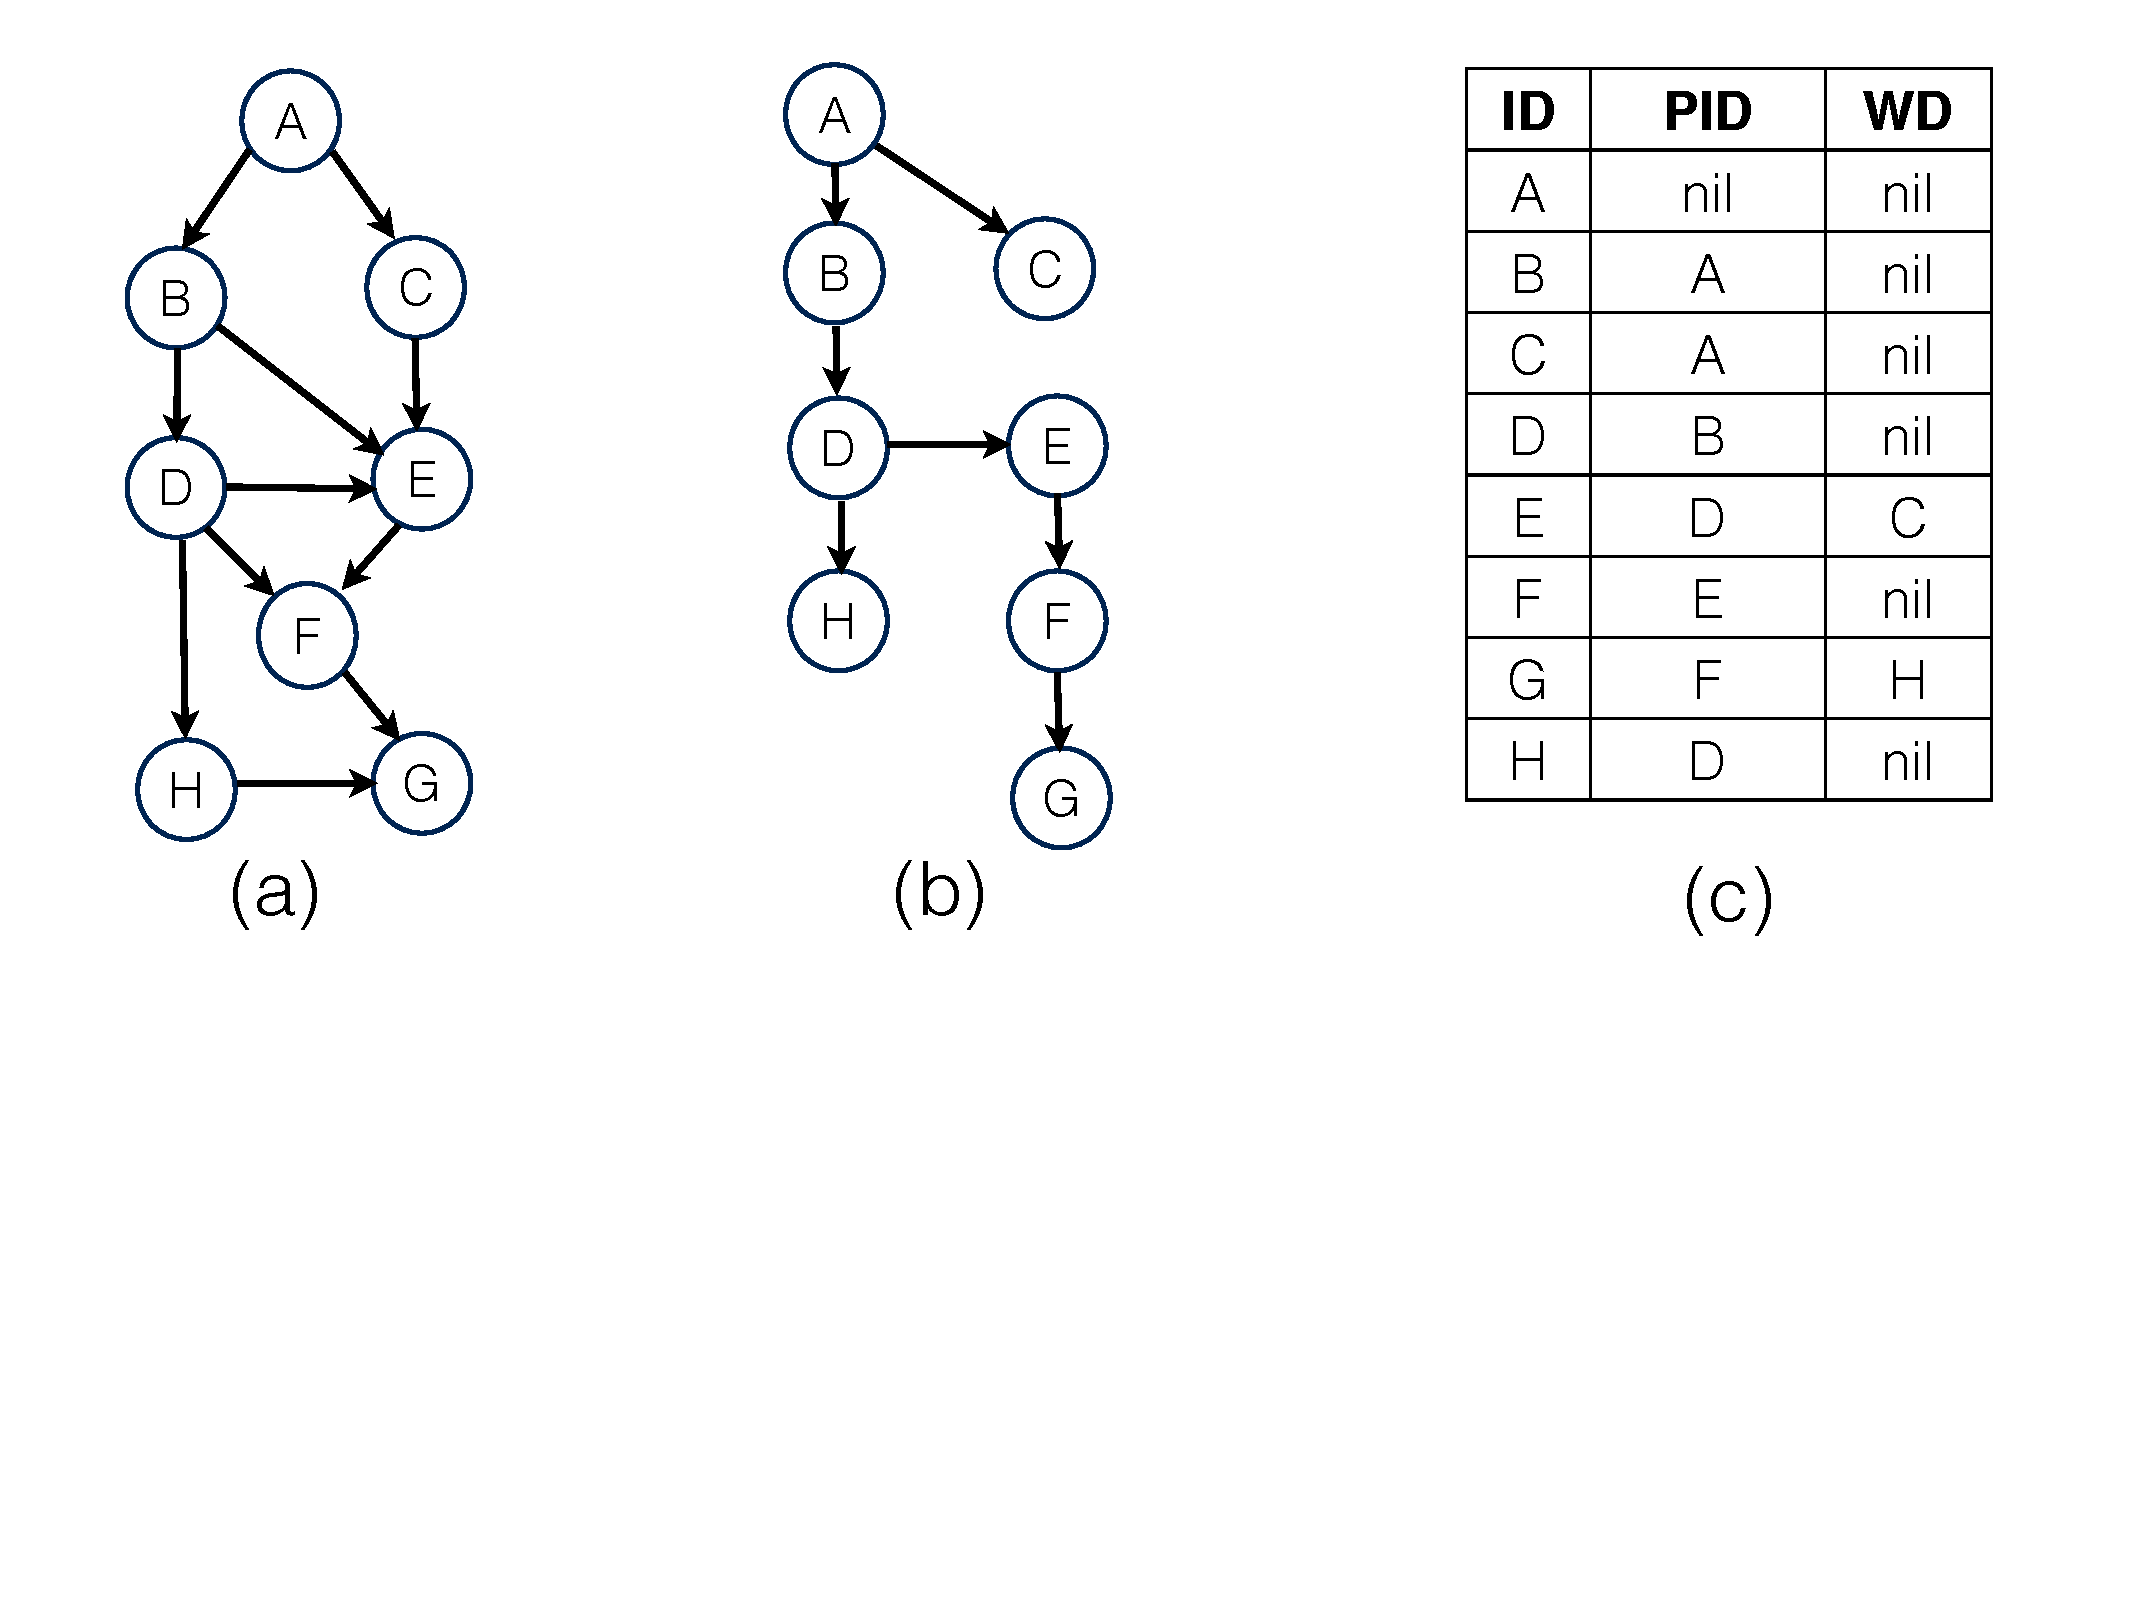
\includegraphics[width=0.8\textwidth]{chapter3/di_indexing.pdf}
	\caption{I-Index Construction over the Pathway DAG in Figure~\ref{fig:topological}. (a) shows the DAG structure; (b) provides the inheritance relationship discovered during the index construction; (c) shows the final I-Index.}
	\label{fig:diff-index}
\end{figure}

\section{Inheritance Index}
\textit{DBIndex} is a general index that can support both k-hop as well as
topological window queries. 
%This is intuitive as the window matrix is able to cover both k-hop window or topological window. 
However, the evaluation of a topological window function, $W_t$, 
can be further optimized due to its containment feature. 
In other words, the window of a descendant vertex 
completely covers that of one of its ancestors. 
This feature can be formally formulated in the following theorem. 

\begin{theorem}
\label{thm:containment}
In a DAG, if vertex u is the ancestor of vertex v, the topological window of $v$, $W_t(v)$ completely contains the window of $u$, $W_t(u)$, i.e., $W_t(u) \subset W_t(v)$.   
\end{theorem}

\begin{proof}
In a DAG, if $u$ is the ancestor of $v$, then $u \leadsto v$. $\forall w \in W_t(u)$, then $w \leadsto u$. As $u \leadsto v$, then $w \leadsto v$. Thus, $w \in W_t(v)$ and the theorem is proved.   
\end{proof}

Let us consider the BioPathway graph in Figure~\ref{fig:topological} as
an example.
Figure~\ref{fig:diff-index} (a) shows its abstract DAG. In (a), 
D is the ancestor of E. In addition, we can see that the window of $D$, 
$W_t(D)$ is $\{A, B, D\}$ and the window of $E$, $W_t(E)$ is $\{A, B, D, C, E\}$. It is easy to see that $W_t(D) \subset W_t(E)$. 

Now, Theorem~\ref{thm:containment} provides us with opportunities for optimizing
the space and computation of topological window queries. 
First, since the set of vertices corresponding to the
window of a node, say $u$, is a superset of the set of vertices of its
parent node, say $v$, there is no need to maintain the full set of 
vertices of the window at $u$. Instead, 
we only need to maintain the difference between 
$W_t(u)$ and $W_t(v)$. We note that in a DAG, it is possible for $u$ to have
multiple parents, $v_1, \cdots, v_k$. In this case, the parent
which has the smallest difference with $u$ can be used; where there
is a tie, it is arbitrarily broken.
We refer to this parent as the {\em closest} parent. For instance, in Figure~\ref{fig:diff-index} (a), instead of maintaining 
$\{A, B, D, C\}$ for $W_t(E)$, it can simply maintain the difference 
to $W_t(D)$ which is $\{C\}$. This is clearly more space efficient.

Second, using a similar logic, the aggregate computation
at a node $u$ can actually reuse the 
aggregate result of its closest parent, $v$.
Referring to our example, the aggregation result of $W_t(D)$ can be 
simply passed or inherited to $W_t(E)$ and further aggregated with the difference 
set ($\{C\}$) in $W_t(E)$ to generate the aggregate value for $W_t(E)$. 
Figure~\ref{fig:diff-index} (b) indicates the inheritance relationship that 
the values of the father can be inherited to the child in the tree. 

Thus, we propose a new structure, called the \textbf{inheritance index}, 
$I$-$Index$, to support efficient processing of topological window queries. 
In $I$-$Index$, each vertex $v$ maintains two information. 
\begin{itemize}
\item The first information is the ID of the closest parent (say $u$) 
of $v$. We denote this as PID($v$).
\item The second information is the difference between 
$W_t(v)$ and $W_t(u)$. We denote this as WD($v$). 
\end{itemize}

With PID($v$), we can retrieve $W_t(u)$, and combining with 
WD($v$), we can derive $W_t(v)$. 
Likewise, we can retrieve the aggregation result of $u$ 
which can be reused to compute $v$'s aggregation result.

Figure~\ref{fig:diff-index}(c) shows the I-index of our example
in Figure~\ref{fig:diff-index}(a). In the figure, I-Index
is represented in a table format; 
the second column is the PID and the third indicates the WD. 

\subsection{Index Construction} 

Building an I-Index for a DAG
can be done efficiently. 
This is because the containment relationship can be easily 
discovered using a topological scan.
Algorithm~\ref{algo:piconstruction} lists the pseudo code for 
index creation. 
The scheme iterates through all the vertices in a topological order.
For vertex $v$, the processing involves two steps.
In the first step, we determine the closest parent
of $v$. This is done by comparing the cardinalities of 
the windows of $v$'s parents, and 
find the parent with largest value. 
The corresponding PID is recorded in the \emph{PID} field of 
I-Index (Lines~\ref{algo:tp-step1-start}-\ref{algo:tp-step1-stop}). 
In the second step, the window of $v$, $W_t(v)$, is pushed to 
its children 
(Lines~\ref{algo:tp-step2-start}-\ref{algo:tp-step2-stop}). 
When the processing of $v$ finishes, its window can be discarded. This
frees up the memory space, which makes the scheme memory efficient.

We not that the complexity of Algorithm~\ref{algo:piconstruction} is non-trivial to analyze. 
This dues to the difficulty of analyzing of the number of ancestors of each vertex. Suppose the 
average number of ancestors for each vertex is $H$, then Algorithm~\ref{algo:piconstruction} is of
complexity $O(H|V|*d)$, where $d$ is the average degree of the graph. This complexity is close to the
output complexity. That is to gather the all vertex-window mapping, at least $O(H|V|)$ elements needs
to be outputted. Thus the indexing time complexity is reasonably efficient.

We further note that the size of \emph{I-Index} is hard to be precisely evaluated. 
This dues to the difficulty of analyzing the window difference. Assume the average size of window difference
is $D$, then the size of \emph{I-Index} is $O(D|V|)$. Although $D$ can be as large $O(|V|)$, our 
experimental results indicate that the index size is always 
comparable to the graph size. We defer this discussion to 
section \ref{sec:experiments}. Furthermore, it is possible to
reduce the index size (should it be a concern) by employing
compression techniques. 

\begin{algorithm}[h]
\label{alg:piconstruction}
\caption{CreateI-Index}
\begin{algorithmic}[1]
\Require Input graph: $G$ 
\Ensure Inheritance Index: $IIndex$ 
\State $IIndex \leftarrow ()$
\State $p \leftarrow ()$ \Comment{stores the window for each vertex}
\State $c \leftarrow ()$ \Comment{stores the cardinality of window for each vertex}
\ForAll{$v \in$ topological order}
\State $WD \leftarrow -\infty$ \Comment{the window difference}
\State $bestu \leftarrow nil$
\ForAll{$u \in v.parent$} \label{algo:tp-step1-start}
	\If{$c[u] > diff$} 
		\State $diff \leftarrow c[u]$
		\State $bestu \leftarrow u$
	\EndIf
\EndFor \label{algo:tp-step1-stop}
\State $IIndex[v].WD \leftarrow WD$
\State $IIndex[v].PID \leftarrow bestu$
\State $p[v] \leftarrow p[v] \cup v$
\ForAll{$u \in v.child$} \label{algo:tp-step2-start}
	\State $p[u] \leftarrow p[u] \cup p[v]$
\EndFor \label{algo:tp-step2-stop}
\State $c[v] \leftarrow |p[v]|$ \Comment{update window cardinality}
\State $p[v] \leftarrow ()$ \Comment{release memory}
\EndFor
\end{algorithmic}
\label{algo:piconstruction}
\end{algorithm}

%In our experiments, we have evaluated various datasets. 
%The experimental results indicate that the index size is always 
%comparable to the graph size. We defer this discussion to 
%section \ref{sec:experiments}. Furthermore, it is possible to
%reduce the index size (should it be a concern) by employing
%compression techniques. 


\subsection{Query Processing using I-Index}

By employing the I-Index, window aggregation can be processed efficiently 
for each vertex according to 
the topological order. Algorithm \ref{alg:dstw-index} 
provides the pseudo code for the query processing. 
Each vertex $v$'s window aggregation value can be calculated 
by using the following formula: 
\begin{equation}
\Sigma (W_t(v)) = \Sigma (W_t(v.PID),\Sigma(v.WD))
\end{equation}
%%% TANKL: this doesn't work for average!! or min or max!!!
%%%%
where $\Sigma$ is the aggregate function. As the vertex is 
processed according to the topological order, $W_t(v.PID)$ 
would have already been calculated while processing $v$'s parent and 
thus can be directly used for $v$ without any recompution. 
In general, $v$'s window aggregation is achieved by utilizing its 
parent's aggregate value and window difference sets. 
This avoids repeated aggregate computation and achieves 
the goal of computation sharing between a vertex and its parent. 
In so doing, the computation overhead can be further reduced. 
Take the index  provided in Figure~\ref{fig:diff-index} (c) as an example, 
assume the query wants to calculate the sum value over each window 
for every vertex. As a comparison, the number of add operations 
are 33, 22, 16 for the cases without any index, 
with DBIndex and with I-Index index respectively. 


\begin{algorithm}
\caption{QueryProcessingOverIIndex}
\begin{algorithmic}[1]
\Require Input graph $G$, aggregate function $\Sigma$, inheritance index $IIndex$ 
\Ensure $w$ \Comment{The aggregation result of each vertex}
\State $w \leftarrow ()$
\ForAll{$v \in$ topological order} \label{code:dstw-index-tp1}
	\State $u \leftarrow IIndex[v].PID$
	\State $WD \leftarrow IIndex[w].WD$
	\State $S \leftarrow v.val$
	\State $S \leftarrow \Sigma(S, w[u])$
	\ForAll{$t \in WD$ } \label{code:dstw-index-tp2}
		\State $S\leftarrow \Sigma(S, t.val)$
	\EndFor
	\State $w[v] \leftarrow S$
\EndFor
\Return $w$
\end{algorithmic}
\label{alg:dstw-index}
\end{algorithm}

As the query processing in Algorithm~\ref{alg:dstw-index} basically scans the \emph{I-Index}, the query
complexity essentially correlates to the index size. As we shown in the experiment session, the query can be performed efficiently 
in various graph conditions. We defer the discussion to Section 6.


\subsection{Handling Updates}
%\remark{
%Similar to DBIndex, attribute updates on I-Index is easy, since I-Index is built on the structure of the graph.
%The general idea for handling structural updates is to identify the region that affected by the structure updates. Because adding or deleting an isolated node is trivial, the core part of structure update is adding/deleting edges. We observe that the region that affected by inserting/deletion edge $e(u,v)$ can be bounded by the subgraph between \emph{Lowest Common Ancestor} of $u,v$ and $v$. Since we do not focus on dynamic graph, we omit the detail here. Interested user may refer to the extended report of this paper \cite{}.}
%\eat{
We cover the updates handling in this section. For attribute updates, \emph{I-Index} is not affected since \emph{I-Index} is only structure related. Structure updates on \emph{I-Index} consists of node updates and edge updates. It is easy to handle the case where an isolated node is added or delete, since it does not affect any other nodes in the graph. Adding (resp. deleting) a node with edges can be done via edge insertions (resp. deletions). Here we focus on describing single edge insertion and deletion. We use $I$ to denote the \emph{I-index} and $I(v)$ to denote the index entry of $v$. 

During an update of edge $e(s,t)$, there are two types of vertices are affected. The first type contains single node $t$, which is the endpoint of edge $e$. The second type of nodes contains all the descendants of $t$. There are altogether four special cases needs to be consider during the updates. We illustrate the four cases with aids of Figure~\ref{fig:dag_update}. In Figure~\ref{fig:dag_update}, the dashed edge $e(s,t)$ is the edge to be updated (added or deleted). The node $u$ is the \emph{lowest common ancestor}(LCA) of $t$ and $s$. The cloud shape $A$ and $B$ are nodes in between of $u,s$ and $u,t$. Since $u$ is the \emph{LCA}, $A$ and $B$ are thus disjoint. Bold edge $e(c,d)$ indicate that $I(d).PID$ is $c$. We distinguish and handle the four cases as follows:

\textbf{Case I ($I(t).PID = s$)}: As shown in Figure~\ref{fig:dag_update} (a), during deletion, $t$ needs to choose a parent from $A$ to be its $I(t).PID$. $I(t).WD$ needs to be updated accordingly. In this case, no insertion needs to be considered since if there is no edge between $s$ and $t$, $I(t).PID$ cannot be $s$. 

\textbf{Case II ($I(t).PID \neq s$)}: As shown in Figure~\ref{fig:dag_update} (b), during insertion, $B$ needs to be excluded from $I(t).WD$. During deletion, any node in $B$ that cannot reach $t$ needs to be included in $I(t).WD$. Since $A$ and $B$ are disjoint, every node in $B$ needs to be removed from $I(t).WD$

\textbf{Case III ($t \leadsto I(v).PID$)}: As shown in Figure~\ref{fig:dag_update} (c), during insertion, any node in $B$ needs to be removed from $I(v).WD$. During deletion, any node in $B$ that reaches $v$ but cannot reach $a$ needs to be added to $I(v).WD$.

\textbf{Case IV ($t \nrightarrow I(v).PID$)}: As shown in Figure~\ref{fig:dag_update} (d), during insertion, any node in $B$ that cannot reach $r$ needs to be included into $I(v).WD$. During deletion, any node in $B$ that cannot reach $v$ needs to be excluded from $I(v).WD$.

During structure updates, essential operations are computing $A,B$ and performing reachability queries. Computing $A,B$ can be done via existing techniques such as \cite{bender2005lowest,czumaj2007faster} while reachability query can be supported by indexing methods such as \cite{yildirim2013dagger}. We defer exploring for more efficient updating algorithms to future work 


\begin{figure*}[t]
\centering
\begin{subfigure}{0.22\linewidth}
  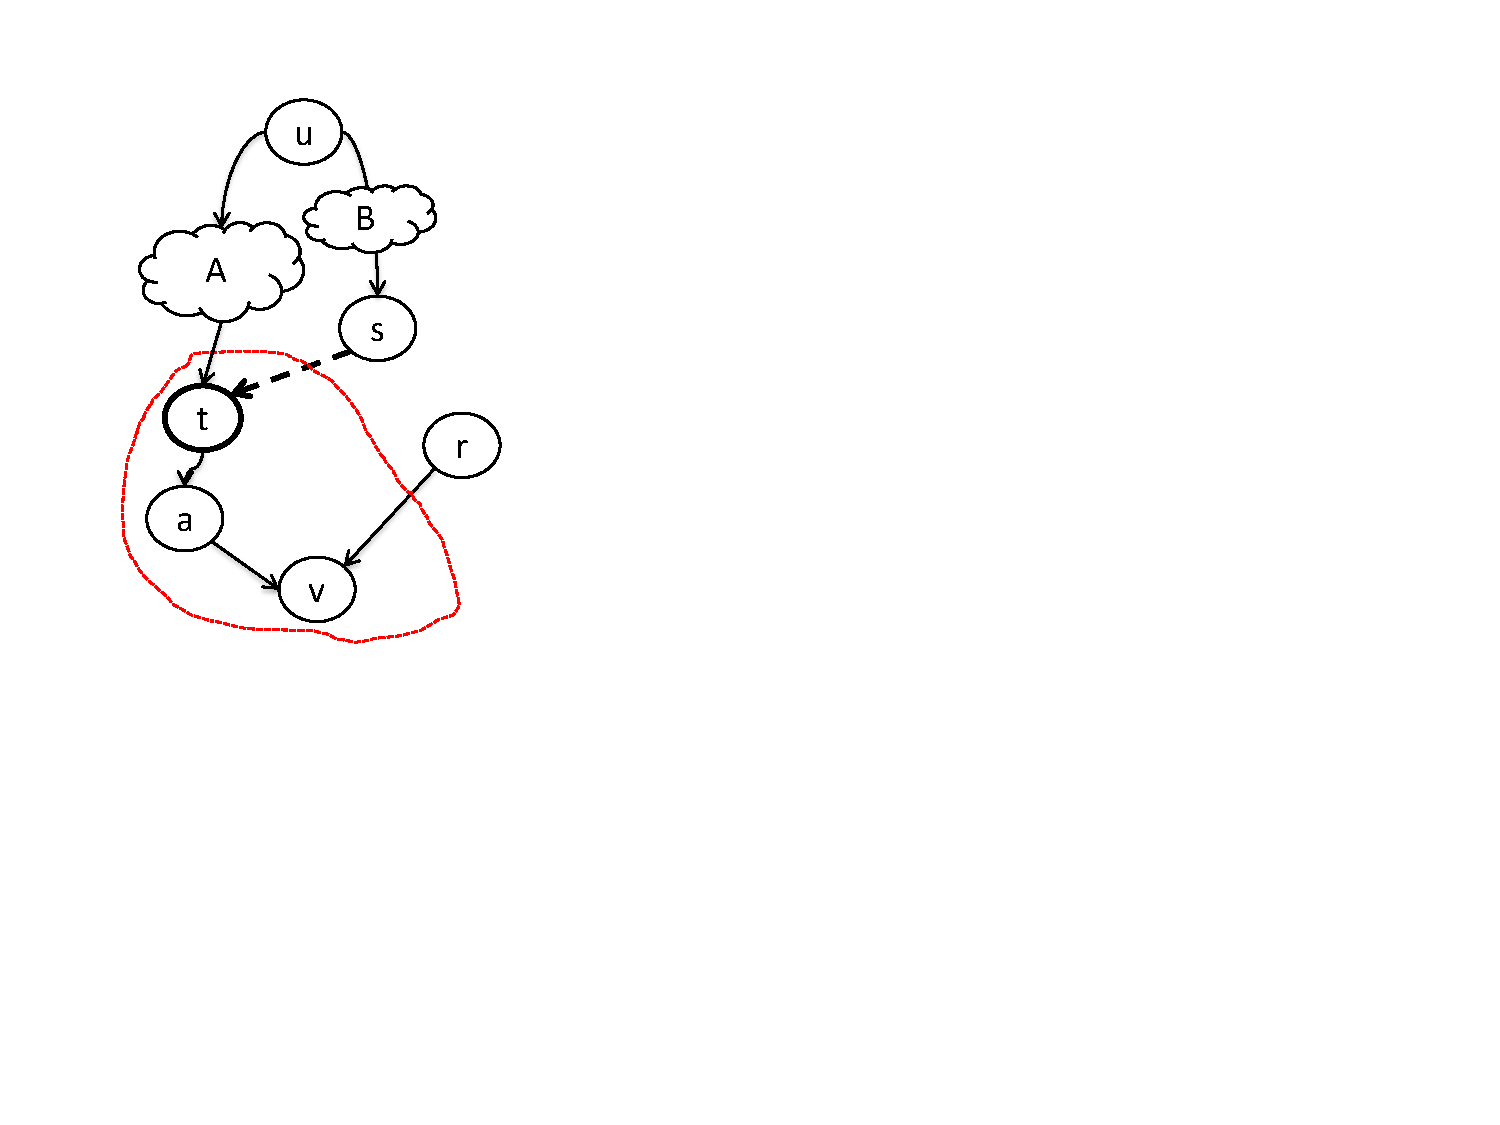
\includegraphics[width=\textwidth]{chapter3/dag_update_1.pdf}
  \caption{Case 1}
\end{subfigure}%
\begin{subfigure}{0.22\linewidth}
  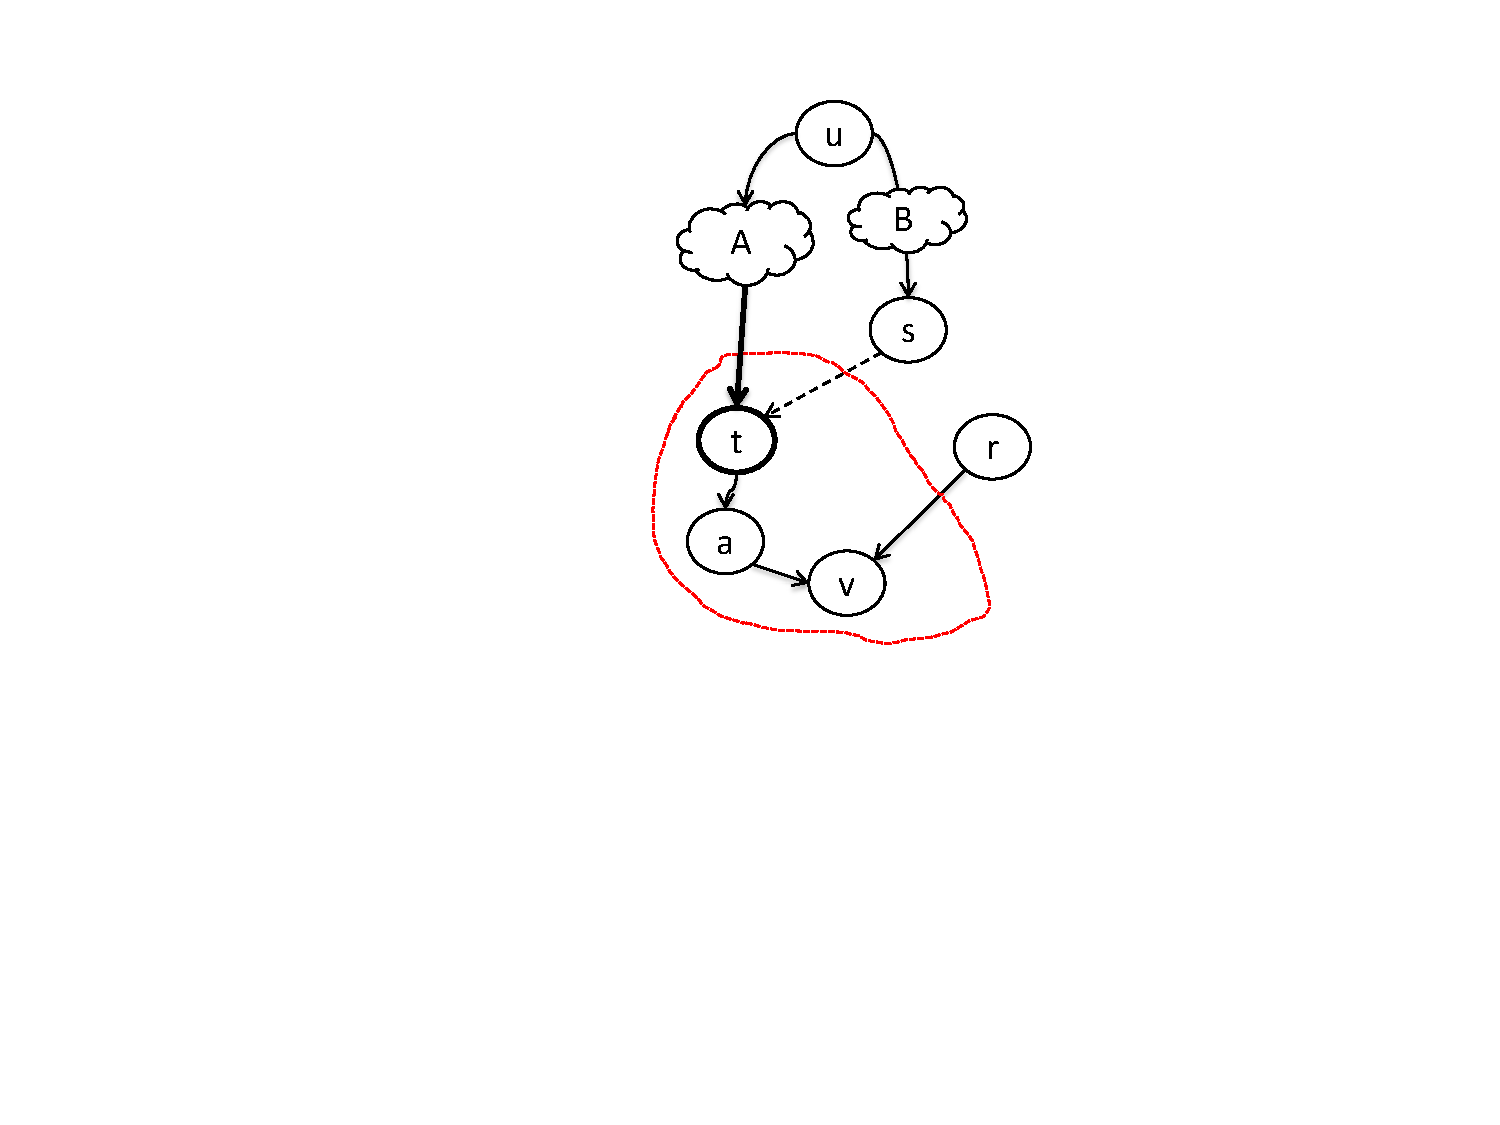
\includegraphics[width=\textwidth]{chapter3/dag_update_2.pdf}
  \caption{ Case 2}
\end{subfigure}
\begin{subfigure}{0.205\linewidth}
  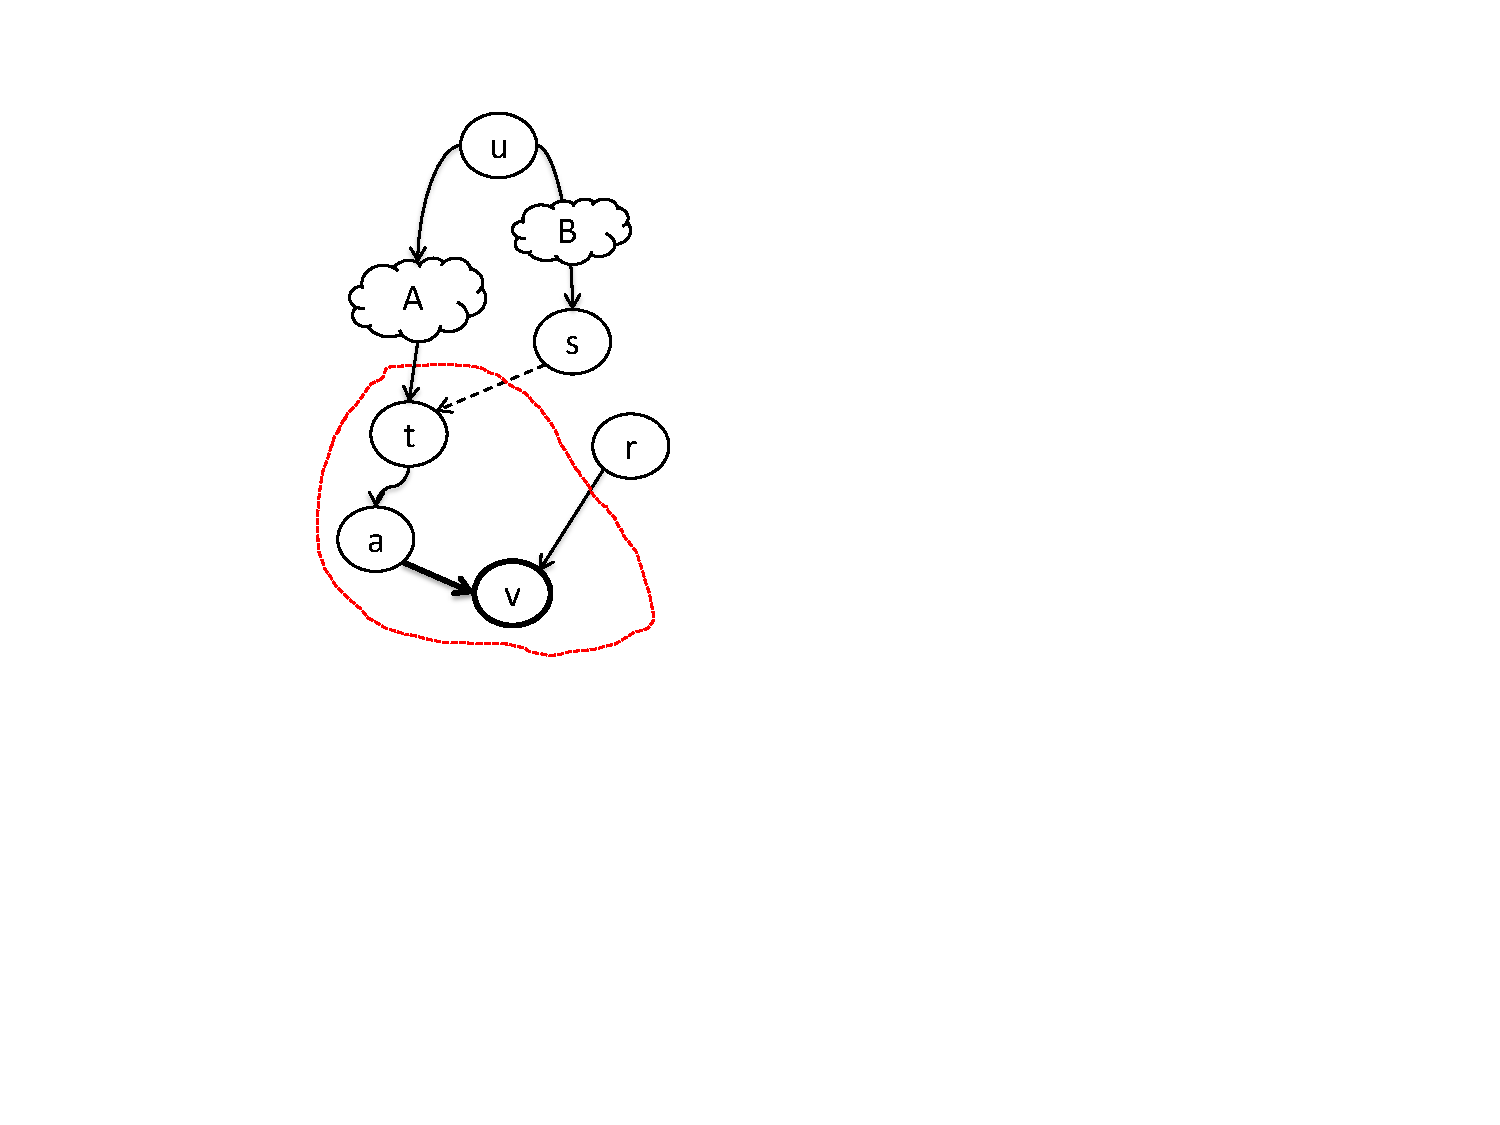
\includegraphics[width=\textwidth]{chapter3/dag_update_3.pdf}
  \caption{Case 3}
\end{subfigure}
\begin{subfigure}{0.22\linewidth}
  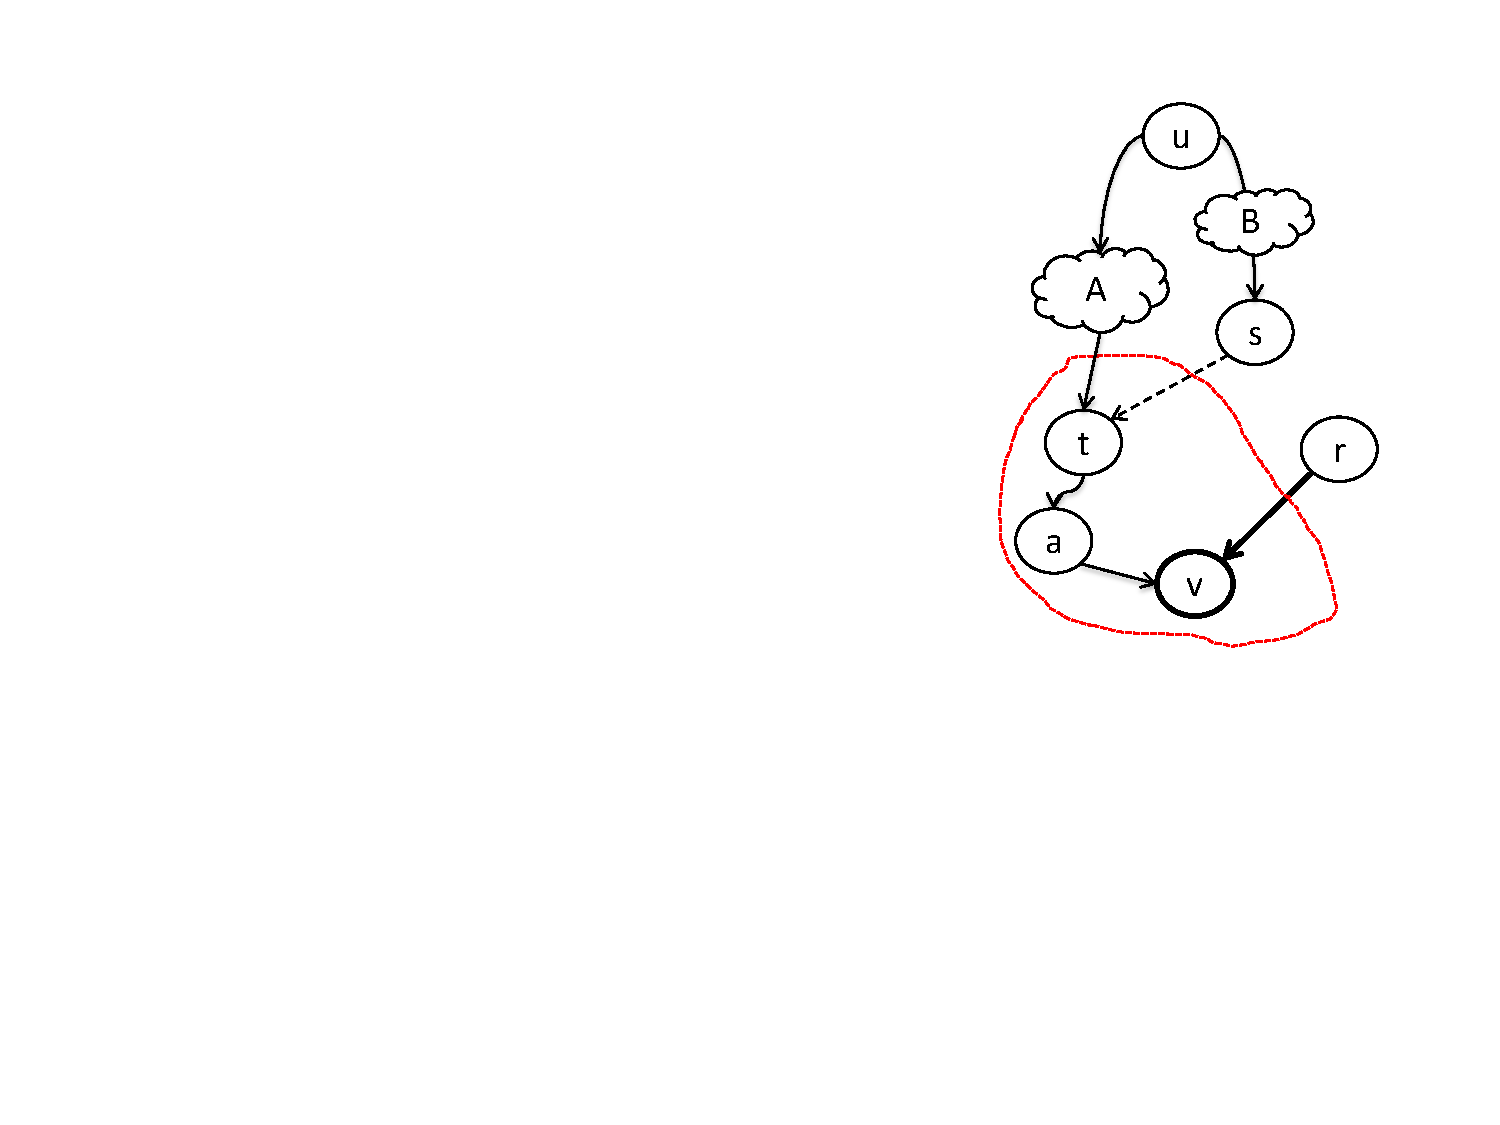
\includegraphics[width=\textwidth]{chapter3/dag_update_4.pdf}
  \caption{Case 4}
\end{subfigure}
\caption{Updates on \emph{I-Index}. Cloud shape indicate the nodes in the subgraph between the endpoint nodes. The dashed circle indicate the affected range of updates. The bold arrow indicates the $PID$ field \emph{I-Index}}
\label{fig:dag_update}
\end{figure*}

%\section{Experimental Evaluation}\label{gw:sec:exp}
In this section, we present a comprehensive experimental evaluation 
of our solutions using several real-world information networks and 
various synthetic datasets. 
%Since the focus of this chapter is on query efficiency, we do not evaluate the efficiency of index updates. 
All experiments are conducted on an 
Amazon EC2 r3.2xlarge machine\footnote{http://aws.amazon.com/ec2/pricing/}, 
with an 8-core 2.5GHz CPU, 60GB memory and 320GB hard drive 
running with 64-bit Ubuntu 12.04. As the source code of EAGR is not
available, we implemented it and used it as a reference in our comparative
study.  
All algorithms are implemented in Java and run under JRE 1.6.

\begin{table}[h]
\caption{Large-scale real graphs.}
\label{tab:realdata}
\centering
\begin{tabular}{|l|l|l|l|}
\hline 
\rule[-1ex]{0pt}{2.5ex} Name & Type & Number of Vertexes & Number of Edges \\ 
\hline 
\rule[-1ex]{0pt}{2.5ex} LiveJournal1 & undirected & 3,997,962 & 34,681,189 \\ 
\hline 
\rule[-1ex]{0pt}{2.5ex} Pokec & directed & 1,632,803 & 30,622,564 \\ 
\hline 
\rule[-1ex]{0pt}{2.5ex} Orkut & undirected & 3,072,441 & 117,185,083 \\ 
\hline 
\rule[-1ex]{0pt}{2.5ex} DBLP & undirected & 317,080 & 1,049,866 \\ 
\hline 
\rule[-1ex]{0pt}{2.5ex} YouTube & undirected & 1,134,890 & 2,987,624 \\ 
\hline 
\rule[-1ex]{0pt}{2.5ex} Google & directed & 875,713 & 5,105,039 \\ 
\hline 
\rule[-1ex]{0pt}{2.5ex} Amazon & undirected & 334,863 & 925,872 \\ 
\hline 
\rule[-1ex]{0pt}{2.5ex} Stanford-web & directed & 281,903 &  2,312,497 \\ 
\hline 
\end{tabular}
\end{table}


\textbf{Datasets.} For real datasets, we use 8 information networks 
which are available at the Stanford \emph{SNAP}\footnote{http://snap.stanford.edu/snap/index.html}: 
LiveJournal1, Pokec, Orkut, DBLP, YouTube, Google, Amazon and Stanford-web. 
The detail description of these datasets is provided in 
Table~\ref{tab:realdata}. 

For synthetic datasets, we use two widely used graph data generators. 
We use the \emph{DAGGER} generator \cite{yildirim2013dagger} to generate 
all the synthetic DAGs and the SNAP graph data generator at the
Stanford SNAP website to generate non-DAG datasets. For each dataset, each vertex is associated with an integer attribute.

\textbf{Query.} In all the experiments, the window query is conducted 
by using the SUM() as the aggregate function over the integer attribute in each dataset. 

\begin{figure*}[t]
\centering
\begin{subfigure}{0.45\textwidth}
  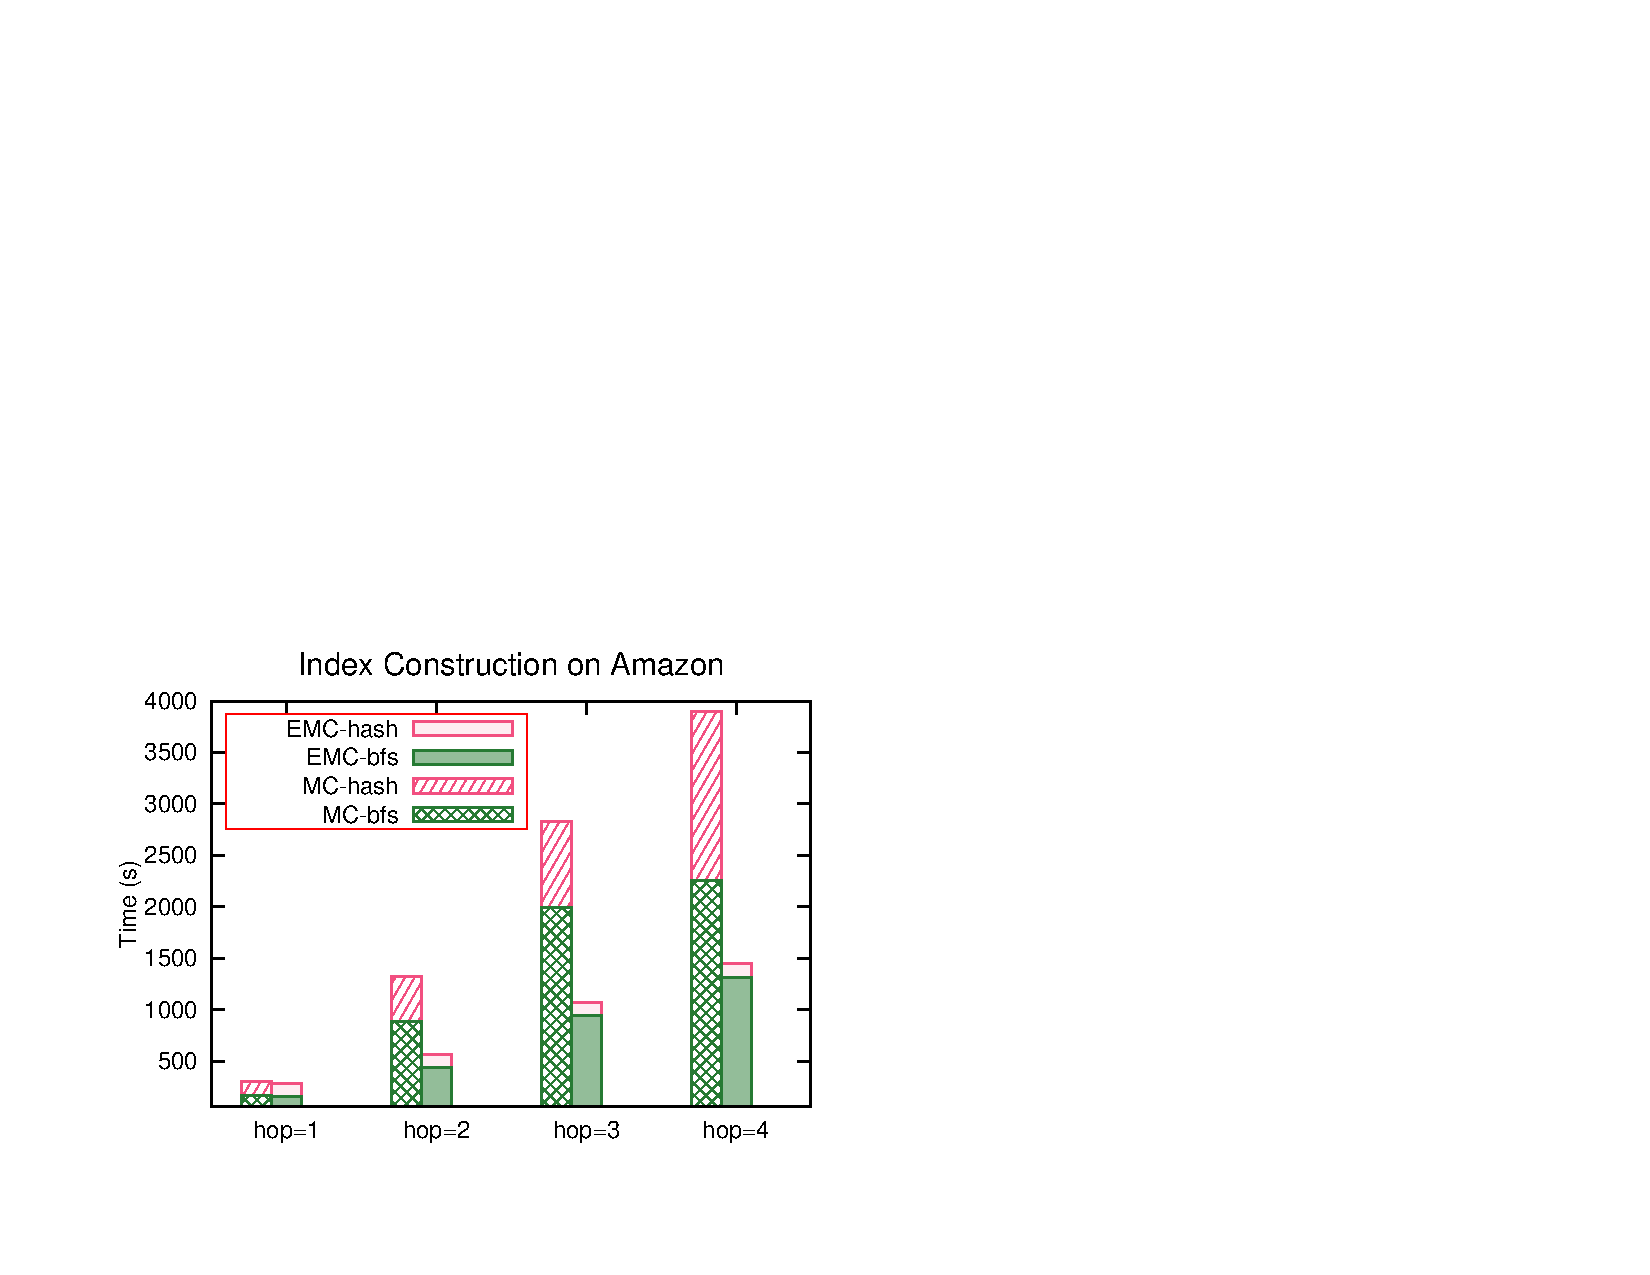
\includegraphics[width=\textwidth]{chapter3/exp/khopeffect/effectiveness/amazon_index_time.pdf}
  \caption{Index built on Amazon}
\end{subfigure}
\begin{subfigure}{0.45\textwidth}
  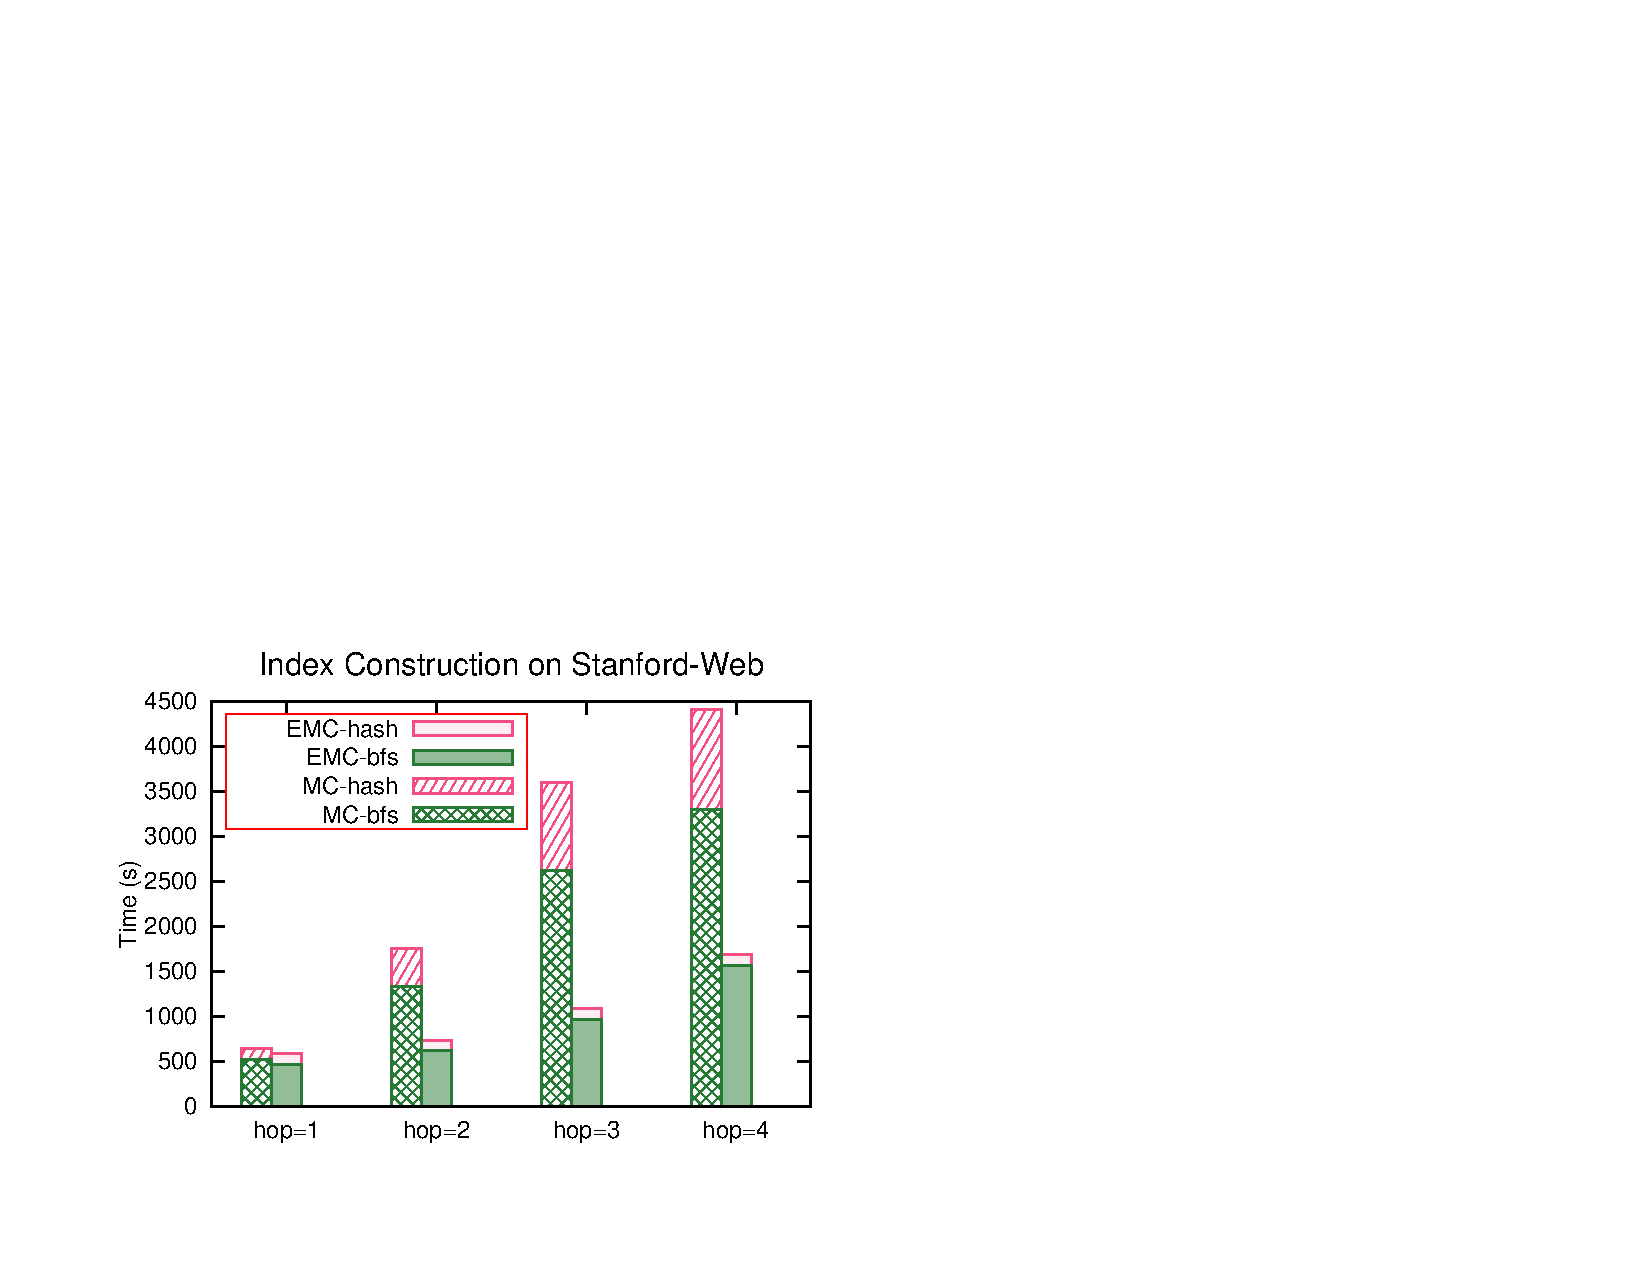
\includegraphics[width=\textwidth]{chapter3/exp/khopeffect/effectiveness/stanford_index_time.pdf}
  \caption{Index built on Stanford-web}
\end{subfigure}

\begin{subfigure}{0.45\textwidth}
  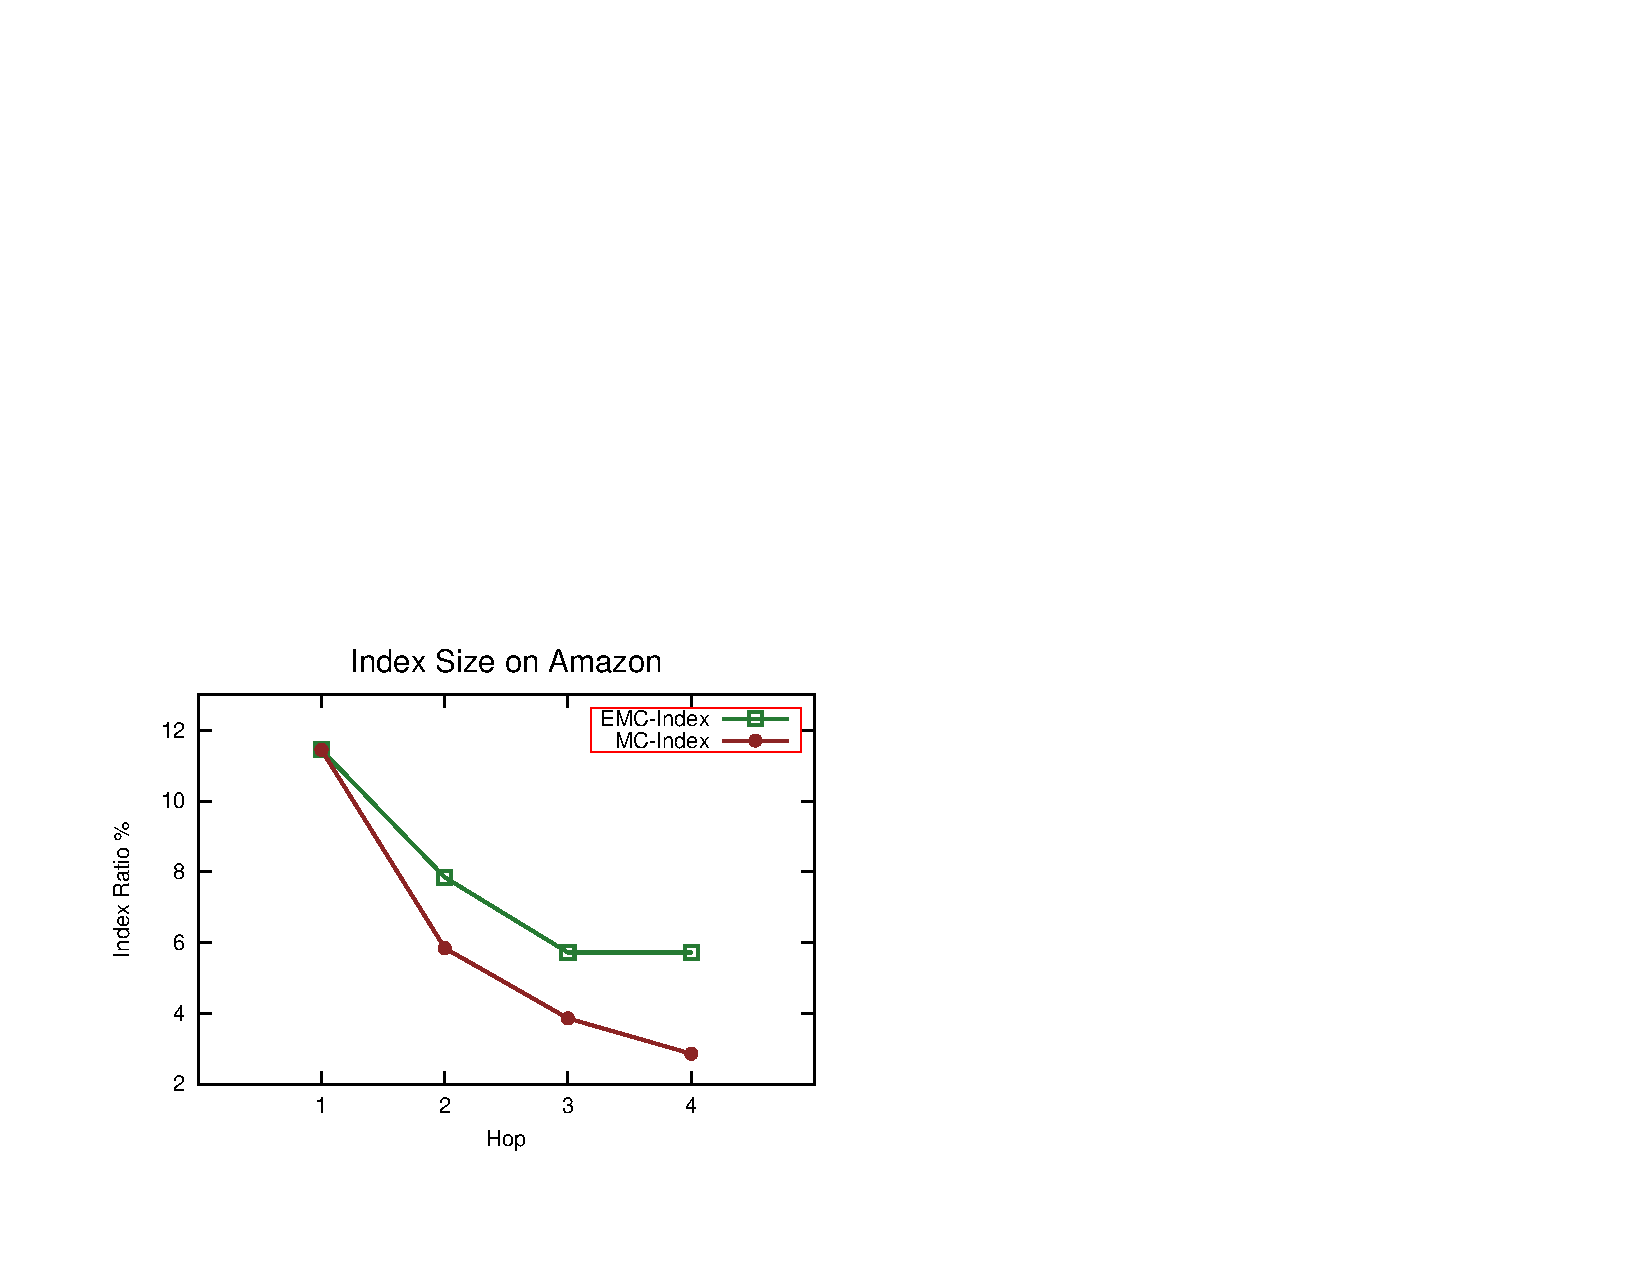
\includegraphics[width=\textwidth]{chapter3/exp/khopeffect/effectiveness/amazon_index_size.pdf}
  \caption{Index size on Amazon}
\end{subfigure}
\begin{subfigure}{0.45\textwidth}
  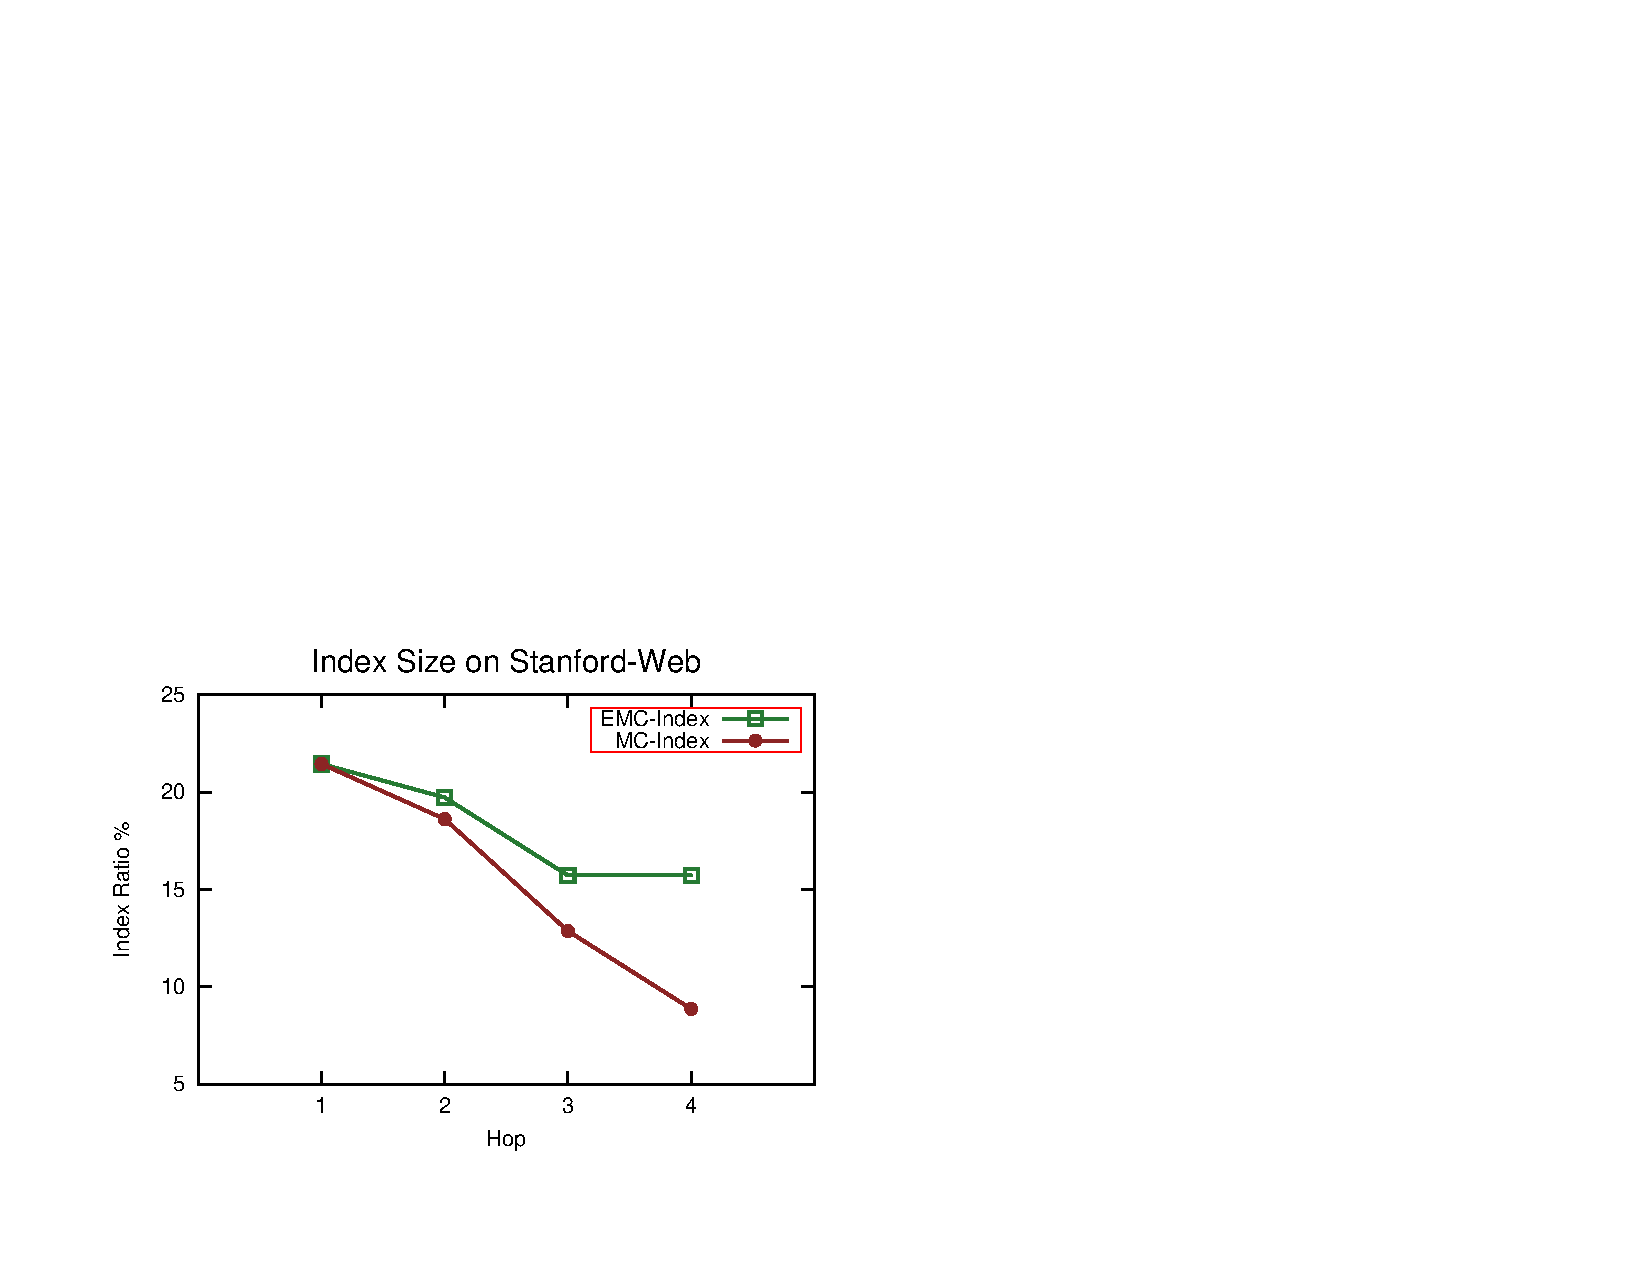
\includegraphics[width=\textwidth]{chapter3/exp/khopeffect/effectiveness/stanford_index_size.pdf}
  \caption{Index size on Stanford-web}
\end{subfigure}
\caption{Index construction analysis for EMC and MC. (a) and (b) 
depict the index time for the Amazon and Stanford-web networks.
(c) and (d) show the index size for the Amazon and Stanford-web datasets.}
\label{fig:index_analysis_emc_mc}
\end{figure*}


\subsection{Comparison between MC and EMC}\label{sec:mc_vs_emc}
We first compare the effectiveness of the two DBIndex 
construction algorithms: MinHash Clustering (MC) and Estimated 
MinHash Clustering (EMC). We look at 
the index construction time, index size and query performance. 
All these experiments are conducted based on two real datasets: 
Amazon and Stanford-web. For both datasets, we run a series of k-hop queries.\footnote{For the Stanford-web graph, which is directed,
the k-hop windows are directed k-hop windows where $u \in W(k)$ if there is a directed path
of at most $k$ hops from vertex $v$ to vertex $u$.
} For queries with hop count larger than 1, 
EMC uses 1-hop information for the initial clustering. 

\textbf{Index Construction. } Figures~\ref{fig:index_analysis_emc_mc} 
(a) and (b) compare the index construction time between MC and EMC 
when we vary the windows from 1-hop to 4-hop for the Amazon and Stanford-web 
graphs respectively. To better understand the time differences, 
the construction time is split into two parts: 
the MinHash cost (EMC-hash or MC-hash) and the breadth-first-search traversal (to compute the $k$-hop window)  cost (EMC-bfs or MC-bfs). The results show the same trend 
for the two datasets. % We make several observations.
First, as the number of hops increases, the index construction time increases as well. 
This is expected as a larger hop count results in a larger window size 
and the BFS and the MinHash time increase correspondingly. 
Second, as the hop count increases, the difference between the
index construction time of EMC and that of MC widens. 
For instance, as shown in Figures~\ref{fig:index_analysis_emc_mc} (a) and (b), for the 4-hop window queries, compared to MC, 
EMC can save $62\%$ and $66\%$ construction time for the Amazon and Stanford-Web datasets respectively.
EMC benefits from both the low MinHash cost and low BFS cost. 
%From Figures~\ref{fig:index_analysis_emc_mc} (a) and (b), 
We can also see that the MinHash cost of MC increases as the number of hops 
increases, while that for EMC remains almost the same as the 1-hop case. 
This shows that the cost of MinHash becomes more significant for larger windows. 
Thus, using 1-hop clustering for larger hop counts reduces the MinHash cost 
in EMC. Similarly, as EMC saves on BFS cost for $k$-hop queries where $k > 1$, 
the BFS cost of EMC is much smaller than that of MC as well. 

\textbf{Index Size.} Figures~\ref{fig:index_analysis_emc_mc} (c) and (d) 
present the effect of hop counts on the index size for the Amazon and Stanford-web 
datasets respectively. The y-axis shows the index ratio which is the index size over the original graph size. 
The insights derived are: 
First, the index size is rather small compared to the original graph: it
varies from $3\%$ to $12\%$ of the original graph for the Amazon dataset 
and from $8\%$ to $22\%$ for the Stanford-web dataset. 
Second, the index size decreases as the number of hops increases. 
While this appears counter-intuitive initially, it is actually reasonable: a larger hop results in a bigger window, which leads
to more dense blocks. Third, the index ratio of EMC is slightly larger 
than that of MC for larger hop count. This indicates that MC can find more dense blocks 
than EMC to reduce the index size. Fourth, the index ratio on 
the Amazon dataset is much smaller than the ones on the Stanford-web dataset. 
This is because the Amazon dataset is undirected while the Stanford-web dataset
is directed. For the Stanford-web dataset, since we use directed k-hop windows, the window size is naturally smaller. 

\begin{figure}[h]
\centering
\begin{subfigure}{0.48\linewidth}
\centering
  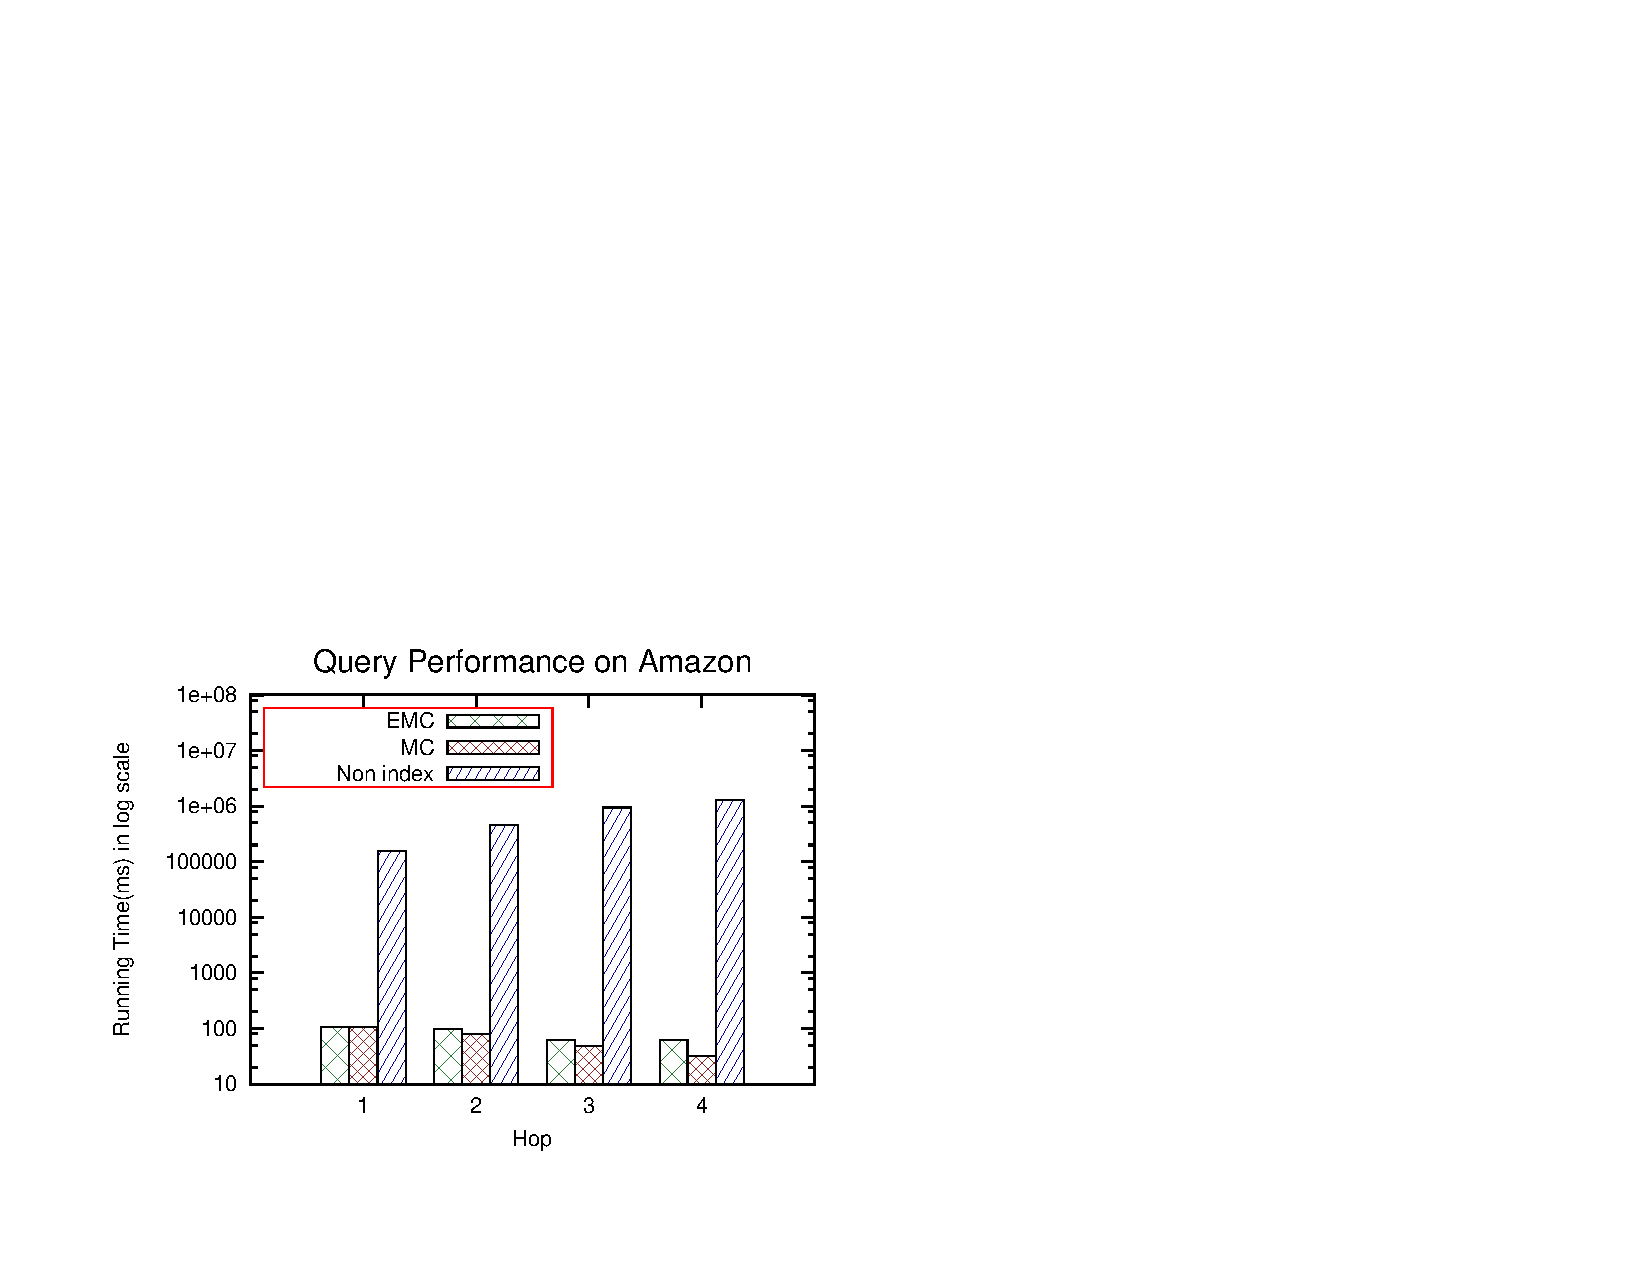
\includegraphics[width=\textwidth]{chapter3/exp/khopeffect/effectiveness/amazon_query_time.pdf}
  \caption{Amazon graph}
\end{subfigure}%
\begin{subfigure}{0.48\linewidth}
\centering
  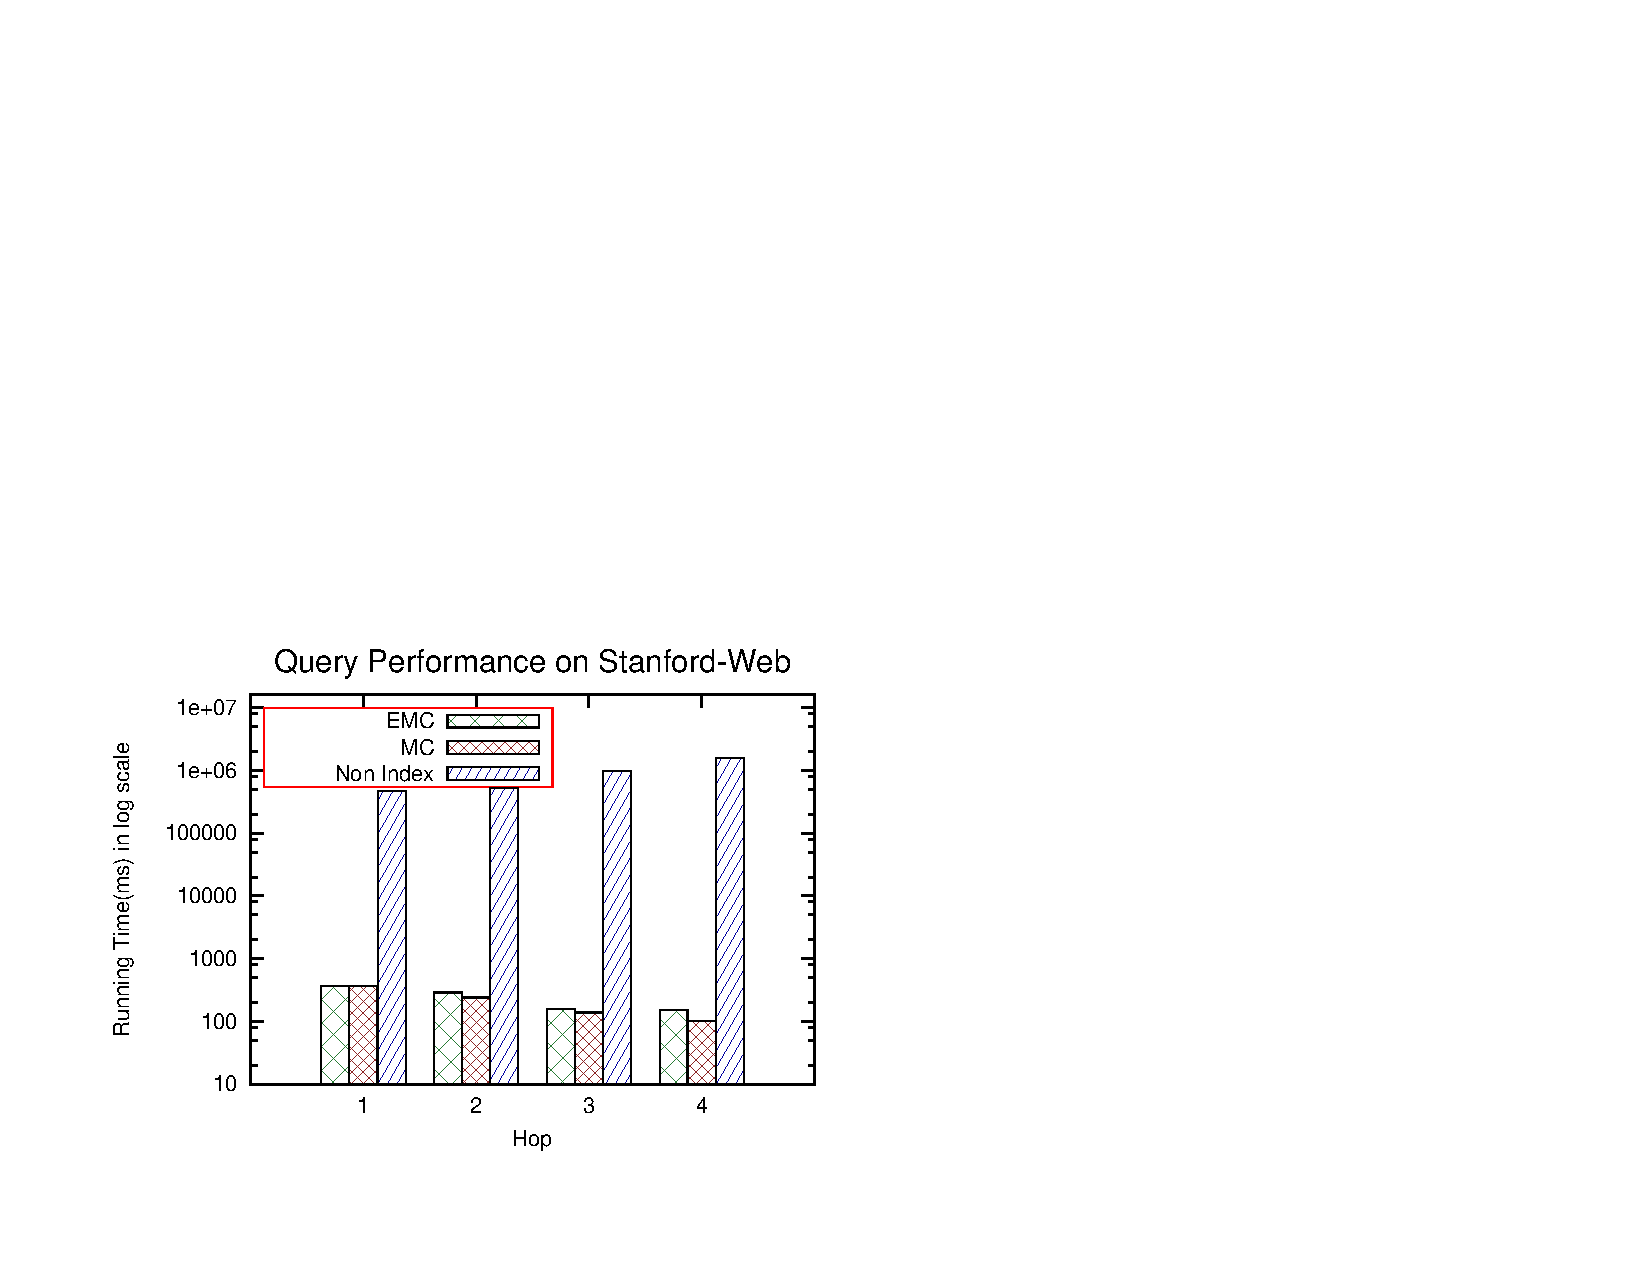
\includegraphics[width=\textwidth]{chapter3/exp/khopeffect/effectiveness/stanford_query_time.pdf}
  \caption{Stanford-web graph}
\end{subfigure}
\caption{Query performance comparison of MC and EMC.}
\label{fig:khop_effective_query_time}
\end{figure}

\textbf{Query Performance.}       
Figures~\ref{fig:khop_effective_query_time} (a) and (b)
present the query time of MC and EMC 
on the two datasets respectively 
as we vary the number of hops from 1 to 4.
To appreciate the benefits of an index-based scheme, we also implemented
a \emph{Non-indexed} algorithm which computes window aggregate by performing $k$-bounded breadth
first search for each vertex individually in run time.
In Figures~\ref{fig:khop_effective_query_time} (a) and (b),
the execution time shown on the y-axis is in log scale. The results show that the index-based 
schemes outperform the non-index approach by four orders of magnitude. 
For instance, for the 4-hop query over the Amazon graph, 
our algorithm is 13,000 times faster than the non-index approach. 
This confirms that it is necessary to have well-designed index support 
for efficient window query processing. By utilizing DBIndex, 
for these graphs with millions of edges, every aggregation query 
can be processed in just between 30ms to 100ms for the Amazon graph and 
between 60ms to 360ms for the Stanford-web graph. In addition, we can 
see that as the number of hops increases, the query time decreases. 
This is the case because a larger hop count eventually results in a larger
number of dense blocks where more (shared) computation can be salvaged. 
Furthermore, we can see that the query time of EMC is slightly longer 
than that of MC when the number of hops is large. This is expected as 
EMC does not cluster based on the complete window information; instead, it
uses only partial information derived from the 1-hop windows. 
However, the performance difference is quite small even for 4-hop queries: for
the Amazon dataset, the difference is only 20ms; and for the Stanford-web
graph, the difference is 35ms. 
For small number of hops, the time difference is even smaller. 
This performance penalty is acceptable as tens of milliseconds time 
difference will not affect user's experience.  As EMC is significantly more 
efficient than MC in index construction, EMC may still be a 
promising solution to many applications. As such, 
in the following sections, we adopt EMC for DBIndex in
our experimental evaluations.  
 

\subsection{Comparison between DBIndex and EAGR}

In this set of experiments, we compare DBIndex and 
EAGR \cite{mondal2014eagr} using both large-scale real 
and synthetic datasets. As described in~\cite{mondal2014eagr},
for each dataset, EAGR runs for 10 
iterations in the index construction.

\begin{figure}[h]
\centering
\begin{subfigure}{0.45\linewidth}
  \centering
  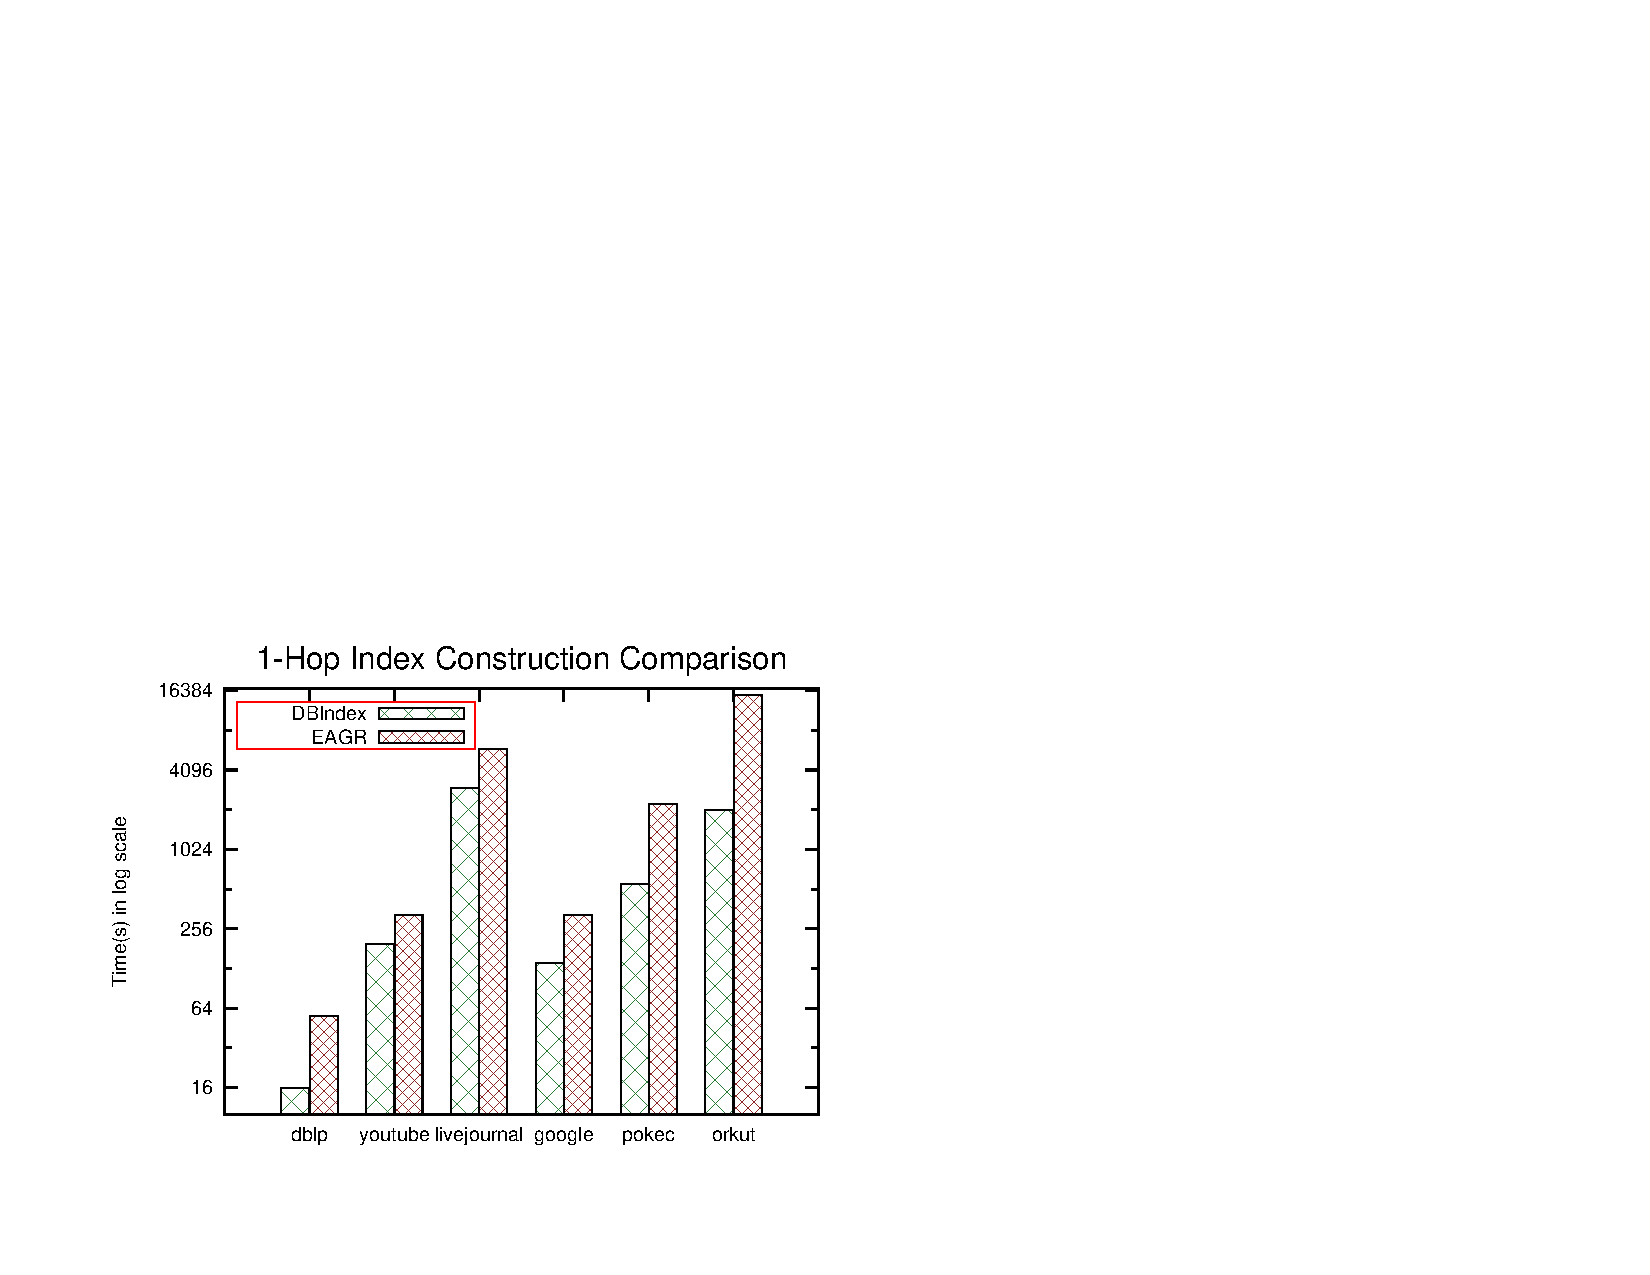
\includegraphics[width=\textwidth]{chapter3/exp/khopeffect/real_data/real_index_time_h1.pdf}
  \caption{1-hop index construction}
\end{subfigure} \begin{subfigure}{0.45\linewidth}
  \centering
  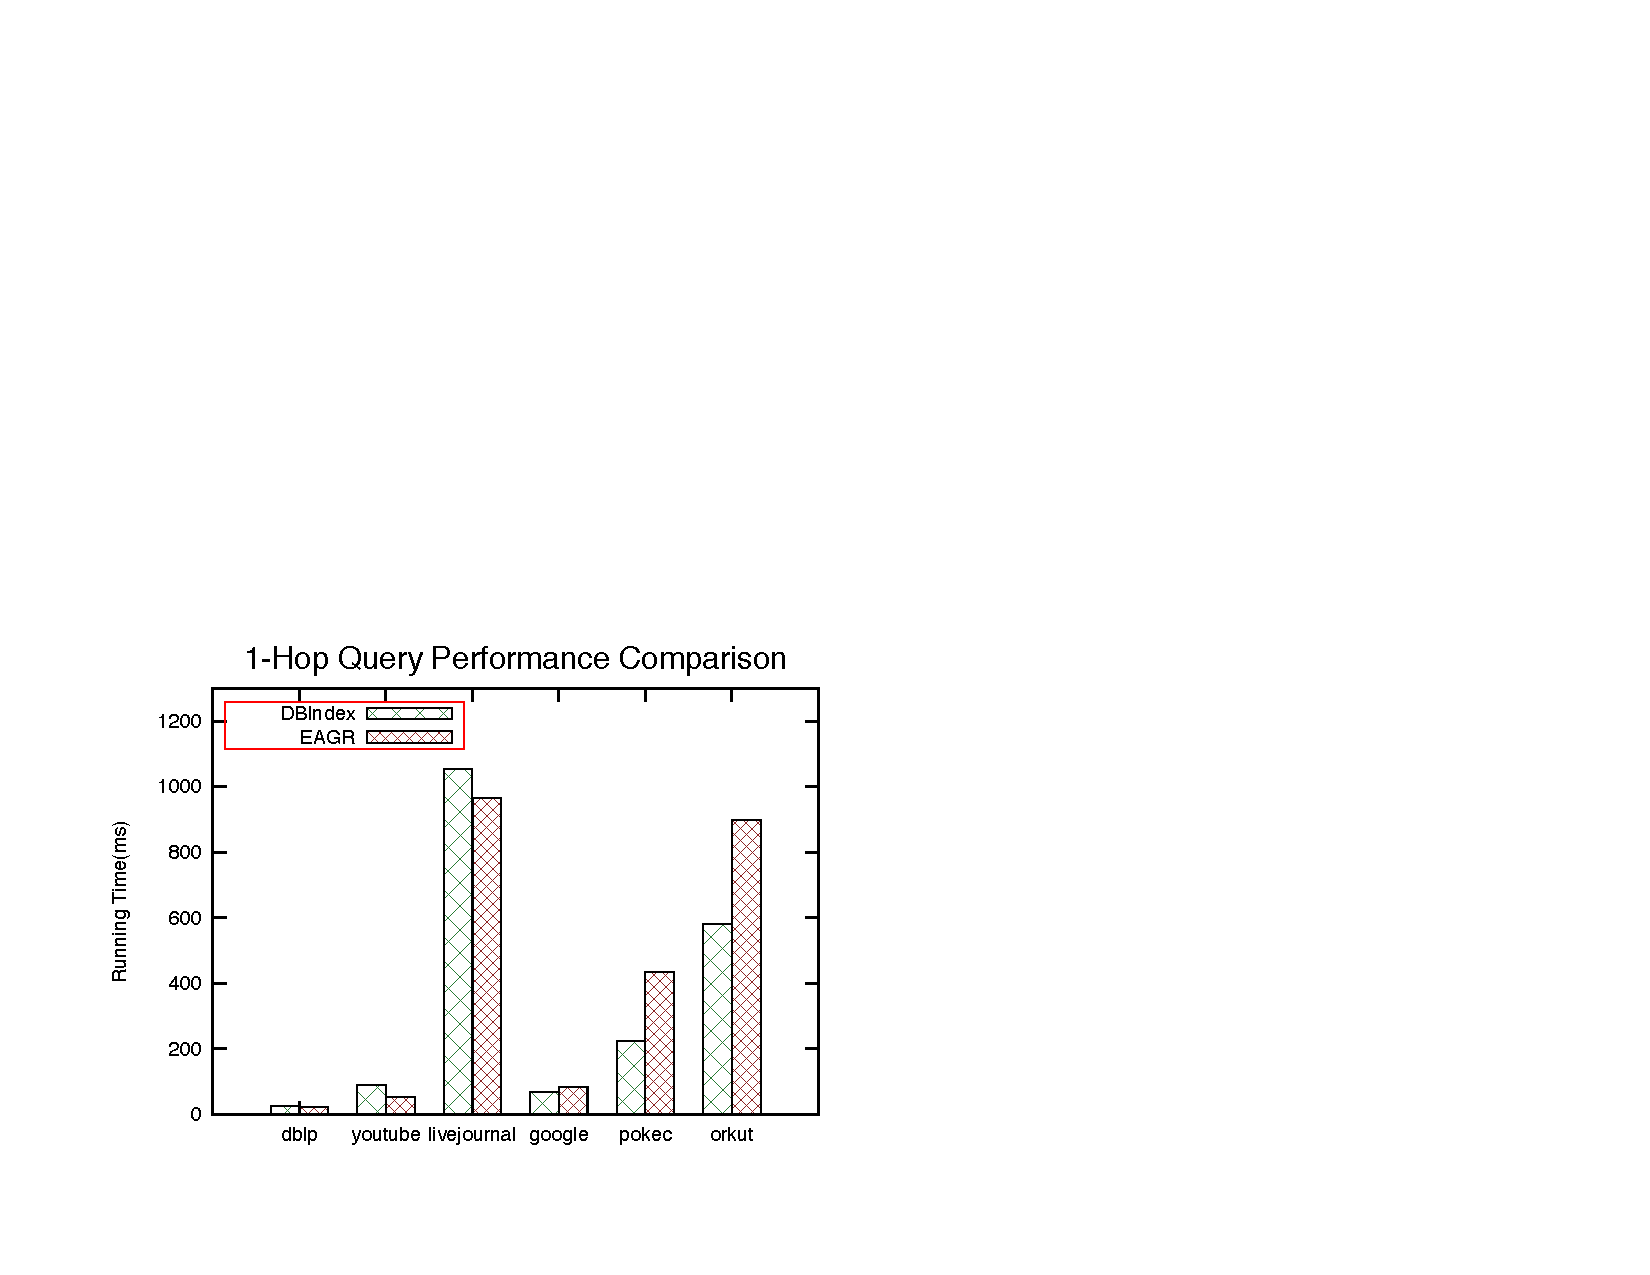
\includegraphics[width=\textwidth]{chapter3/exp/khopeffect/real_data/real_query_time_h1.pdf}
  \caption{1-hop query performance}
\end{subfigure}%
\caption{Comparison between DBIndex and EAGR  for 1-hop query.}
\label{fig:1-hop-real}
\end{figure}

\begin{figure}[h]
\centering
\begin{subfigure}{0.45\linewidth}
  \centering
  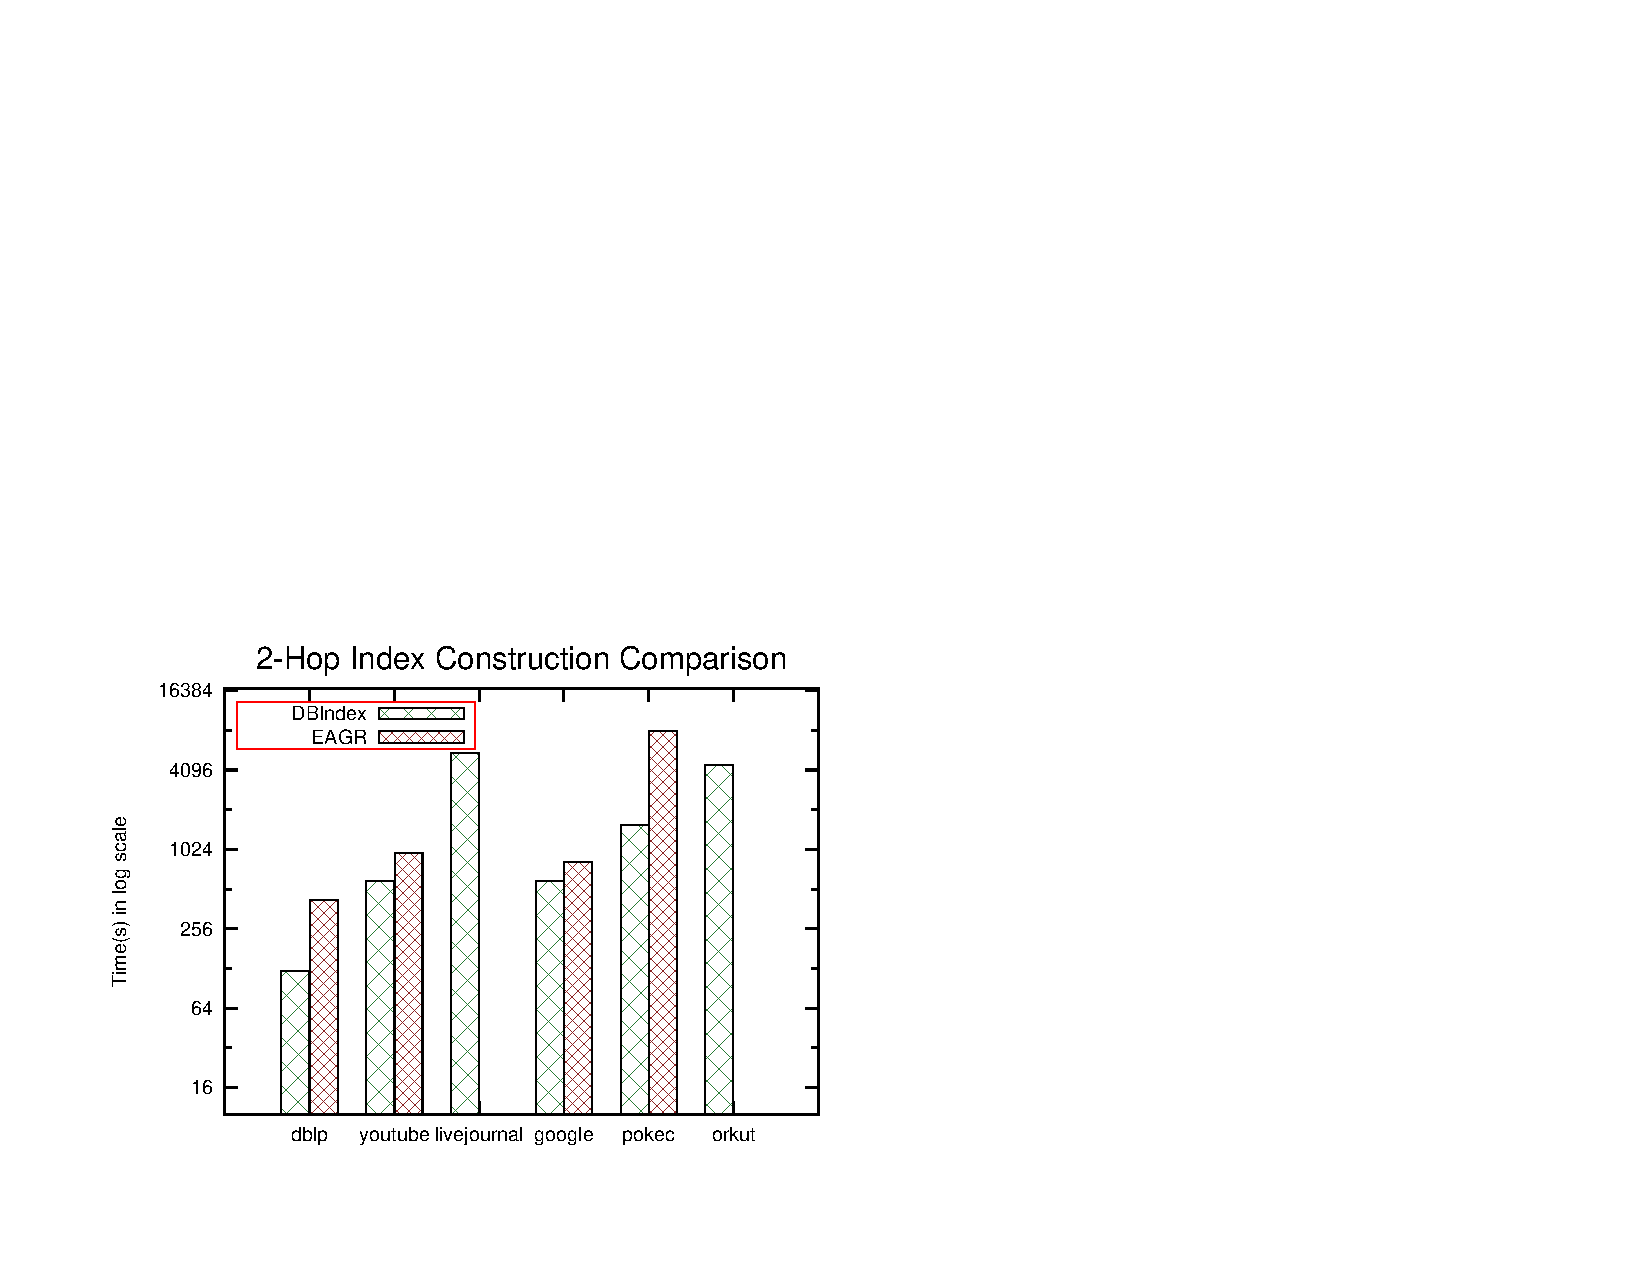
\includegraphics[width=\textwidth]{chapter3/exp/khopeffect/real_data/real_index_time_h2.pdf}
  \caption{2-hop index construction}
\end{subfigure}
\begin{subfigure}{0.45\linewidth}
  \centering
  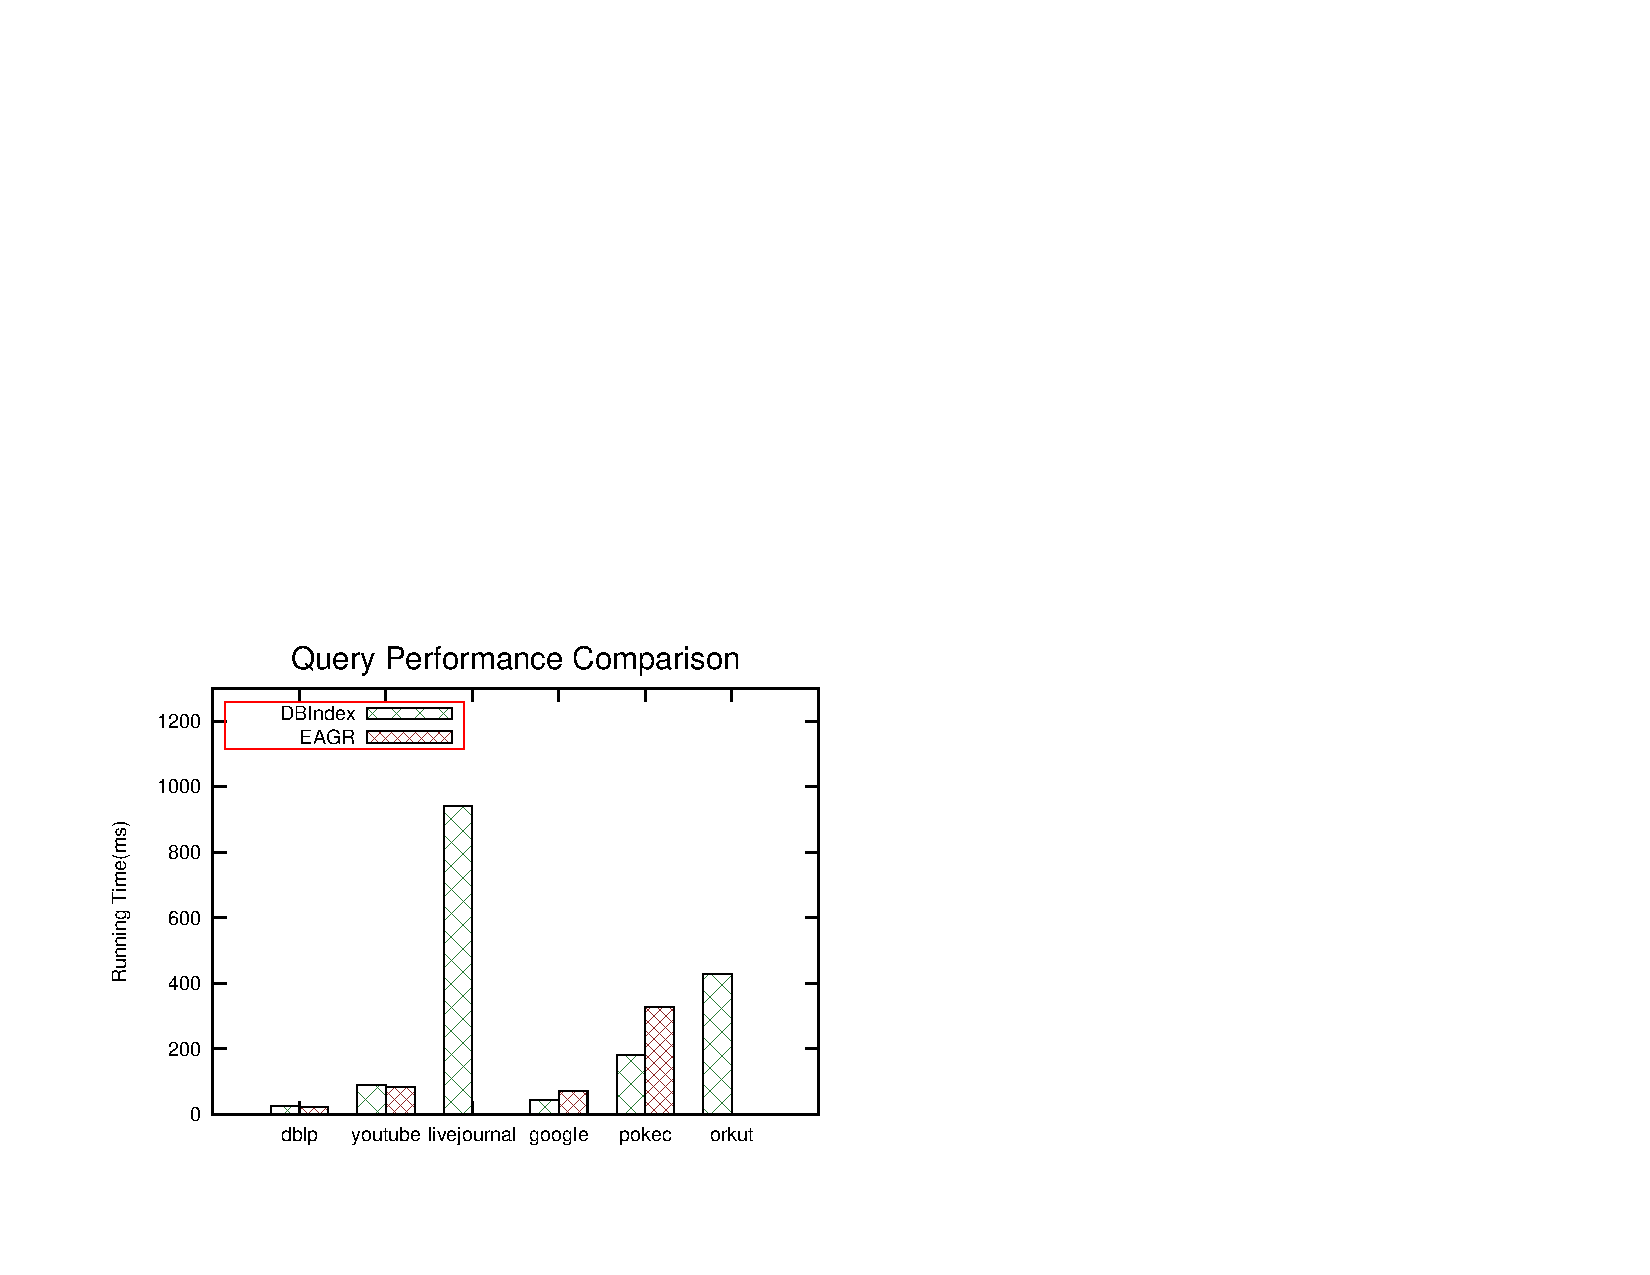
\includegraphics[width=\textwidth]{chapter3/exp/khopeffect/real_data/real_query_time_h2.pdf}
  \caption{2-hop query performance}
\end{subfigure}
\caption{Comparison between DBIndex and EAGR for 2-hop query.}
\label{fig:2-hop-real}
\end{figure}

\subsubsection{Real Datasets} 
We first study the index construction and 
query time performance of DBIndex and EAGR for 1-hop and 2-hop windows 
using 6 real datasets: DBLP, Youtube, Livejournal, Google, Pokec and Orkut. 
The results for 1-hop window and 2-hop window are presented
in Figures~\ref{fig:1-hop-real} and~\ref{fig:2-hop-real} 
respectively. 
As shown in Figures~\ref{fig:1-hop-real}(a) and~\ref{fig:2-hop-real}(a), both DBIndex and EAGR can build the index for all
the real datasets for the 1-hop but EAGR runs out of the memory for the 2-hop query on LiveJournal and Orkut datasets. This further confirms that EAGR incurs 
high memory usage as it needs to build the FP-Tree and 
maintain the vertex-window mapping information. We also observe that 
DBIndex is significantly faster than EAGR in index creation. 
We emphasize that the time is shown in logarithmic scale. 
For instance, for Orkut dataset, EAGR takes 4 hours to build the index 
while DBIndex only takes 33 minutes. 

Figure~\ref{fig:1-hop-real} (b) and Figure~\ref{fig:2-hop-real} (b) 
show the query performance for 1-hop and 2-hop queries respectively. 
The results indicate that the query performance is comparable. 
For most of the datasets, DBIndex is faster than EAGR.
In some datasets (e.g. Orkut and Pokec), DBIndex performs 30\% faster than the EAGR. 
We see that, for the 1-hop query on 
Youtube and LiveJournal datasets and the 2-hop query 
on Youtube dataset, DBIndex is slightly slower than EAGR. We observe 
that these datasets are very sparse graphs where the intersections among windows are naturally small. For very sparse graphs, 
both DBIndex and EAGR are unable to find much computation sharing. In this case, the performance of DBIndex and EAGR is very close. For instance, in the worst case of Livejournal, DBIndex is 9\% slower than EAGR where the actual time difference remains tens of milliseconds.    
%
Another insight is that as expected, compared to Figure~\ref{fig:1-hop-real} (b), 
the 2-hop query runs faster for both algorithms. This is because there is more computation sharing for the 2-hop query. 

In summary, 
DBIndex takes much shorter time to build but offers comparable, if not much faster, query 
performance than EAGR.


\subsubsection{Synthetic Datasets}
To study the scalability of DBIndex under large-scale graphs, 
we generated synthetic datasets using the SNAP generator. 

% streching from 2M vertices to 10M vertices. To see the scalability of our index, we perform extensive tests from both degree and vertex angle.  All data are generated from SNAP\footnote{http://snap.stanford.edu/snap/download.html} graph generator program. We use EAGR as a comparison method. We reported our findings below:

\textbf{Impact of Vertexes.} First, we study how the performance 
changes when we fix the degree\footnote{Degree means average degree of the graph. The generated graph is of Erdos-Renyi model } at 10 and vary the number of vertexes from 
2M to 10M. Figures~\ref{fig:khop_d10_h1} (a) and (b) show the execution time for index construction and query performance respectively. 
From the results, we can see that DBIndex outperforms EAGR in
both index construction and query performance. For the graph with 10M vertexes and 100M edges, the DBIndex query time is less than 450 milliseconds. 
%The increment of DBIndex query with respect to vertex is also steady. 
Moreover, when the number of vertexes changes from 2M to 10M, 
the query performance only increases 3 times. This shows that
DBIndex is not only scalable, but offers acceptable performance. Figures~\ref{fig:khop_d10_h1} (c) and (d) show the
performance of DBIndex in processing the 2-hop query. We notice that EAGR fails to run due to the high memory requirement. For instance, when vertex equals to 2M, the 2-hop query generates 90GB intermediate data, which exceeds the available memory
.

\begin{figure}[t]
\centering
\begin{subfigure}{0.45\linewidth}
  \centering
  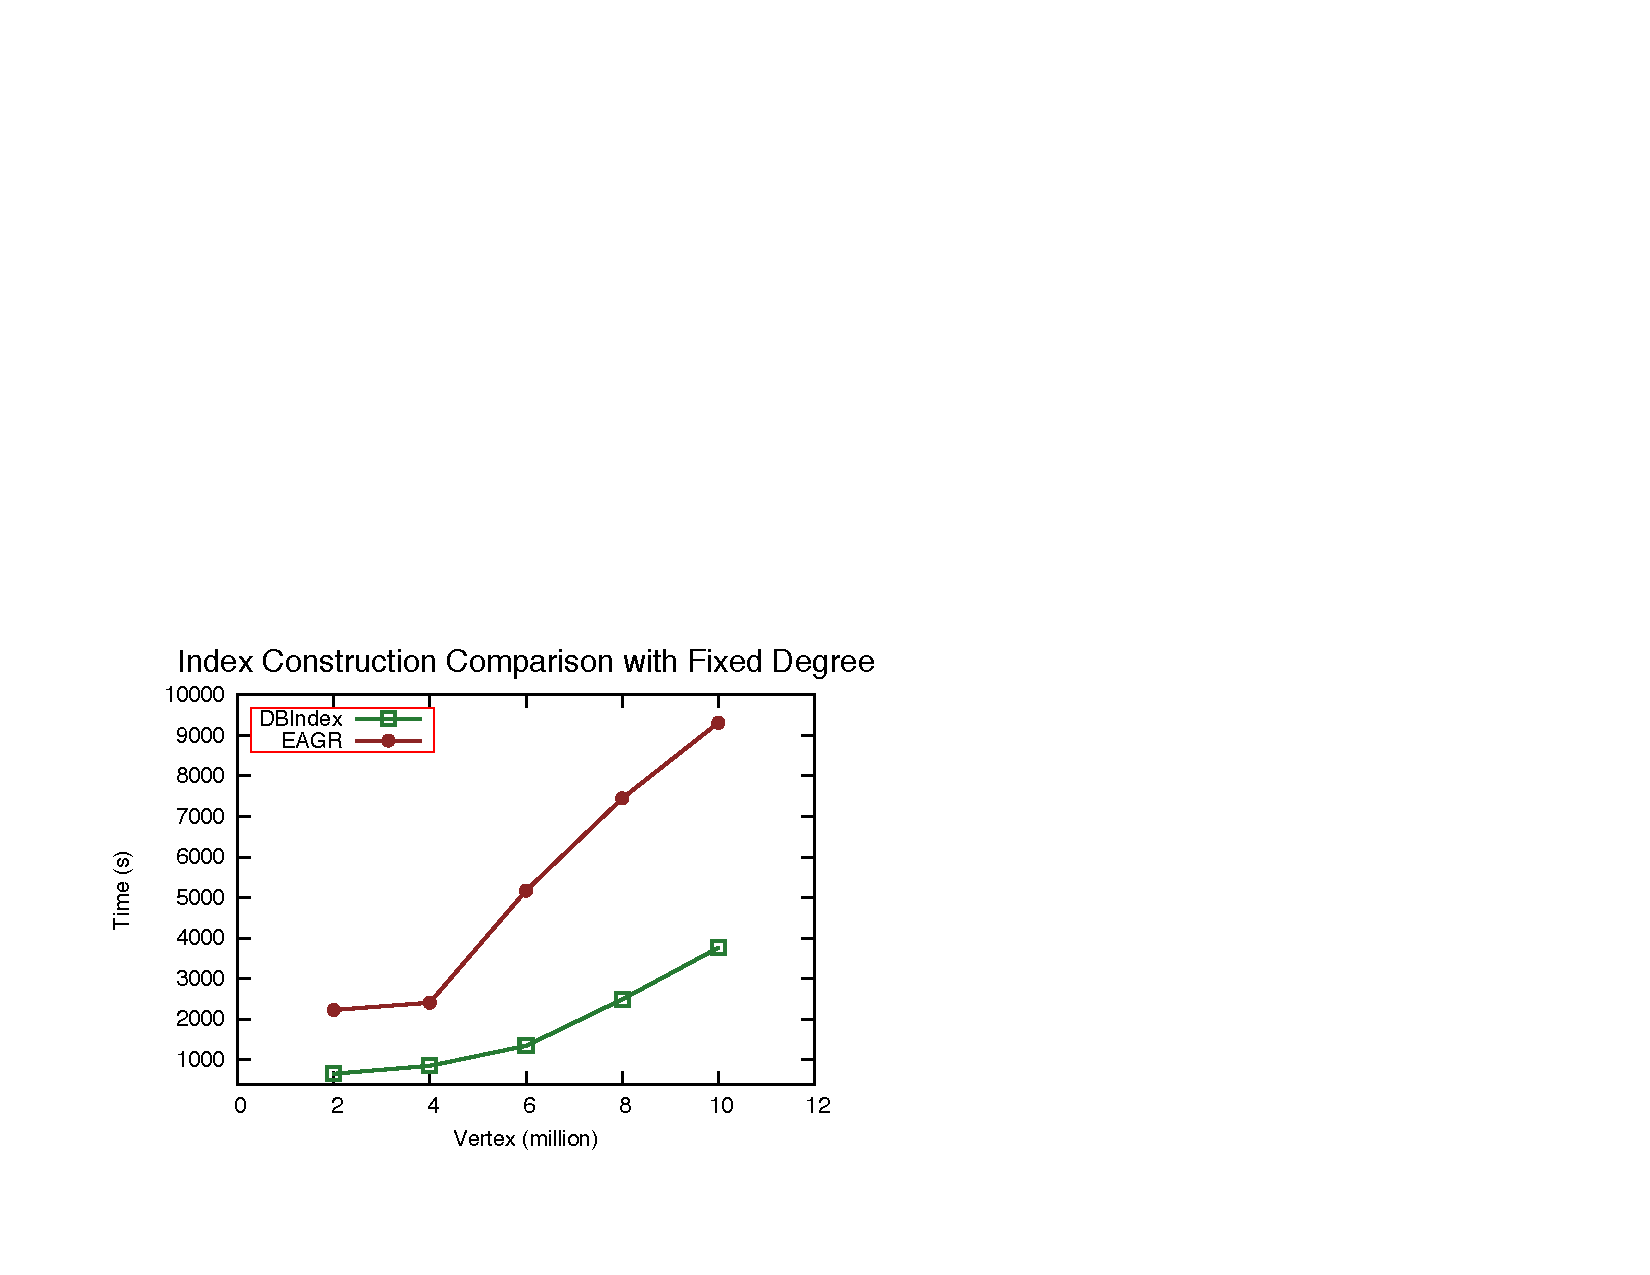
\includegraphics[width=\textwidth]{chapter3/exp/khopeffect/scalability/d10h1_index.pdf}
  \caption{1-hop index construction}
\end{subfigure}
\begin{subfigure}{0.45\linewidth}
  \centering
  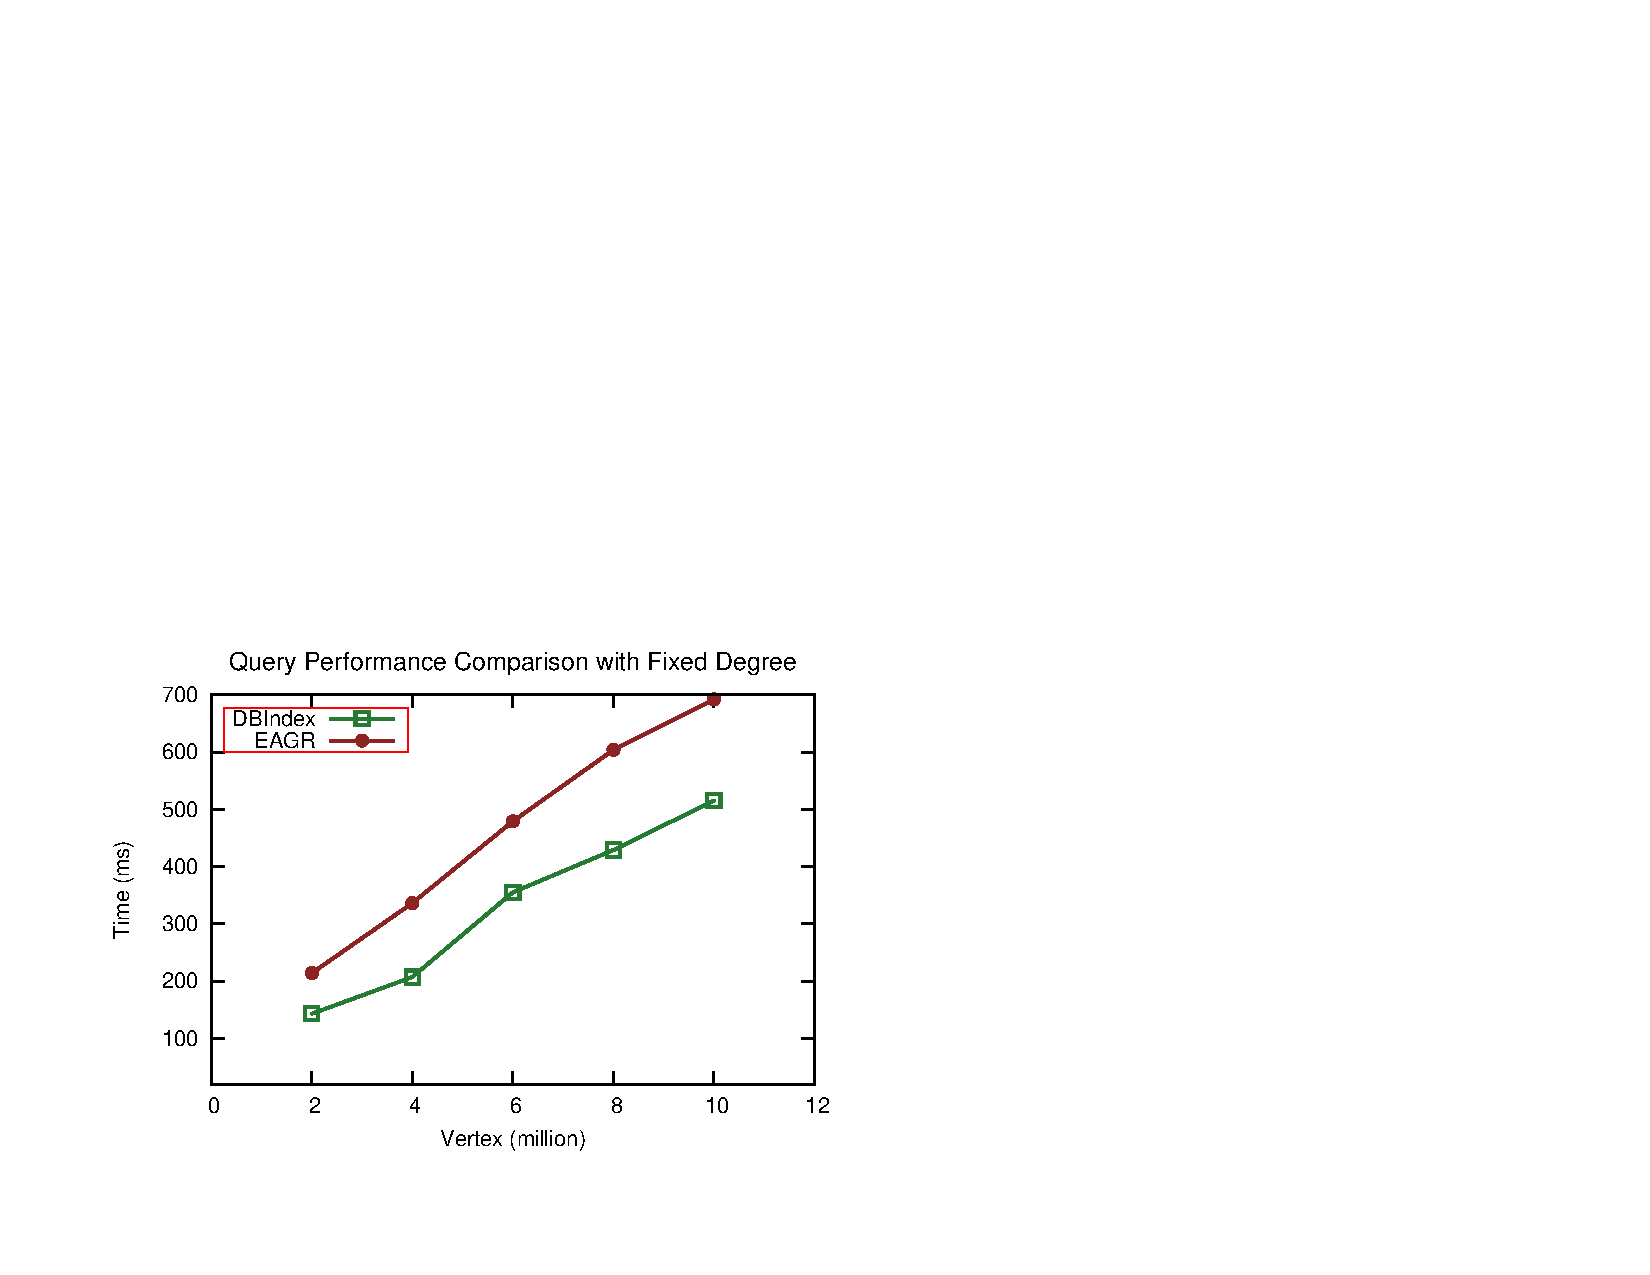
\includegraphics[width=\textwidth]{chapter3/exp/khopeffect/scalability/d10h1_query.pdf}
  \caption{1-hop query performance}
\end{subfigure}
\begin{subfigure}{0.45\linewidth}
  \centering
  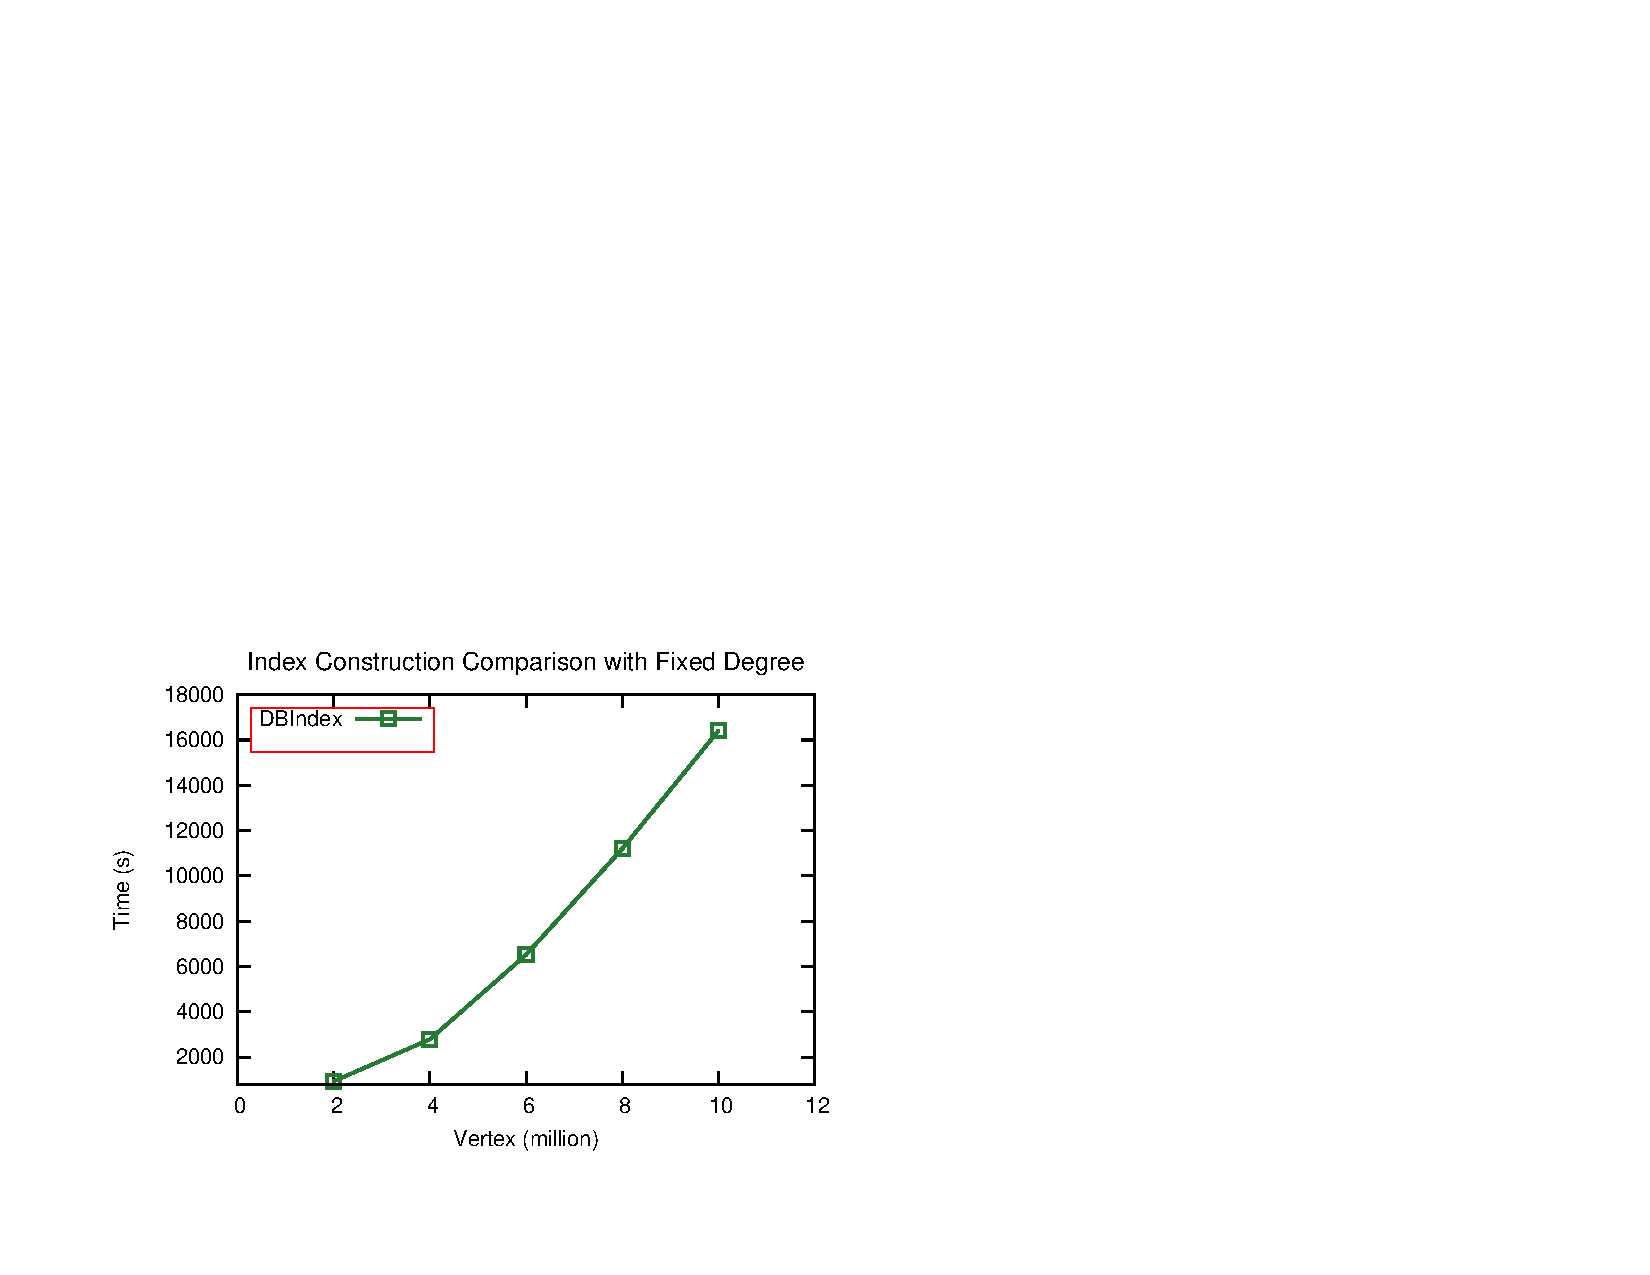
\includegraphics[width=\textwidth]{chapter3/exp/khopeffect/scalability/d10h2_index.pdf}
  \caption{2-hop index construction}
\end{subfigure}
\begin{subfigure}{0.45\linewidth}
  \centering
  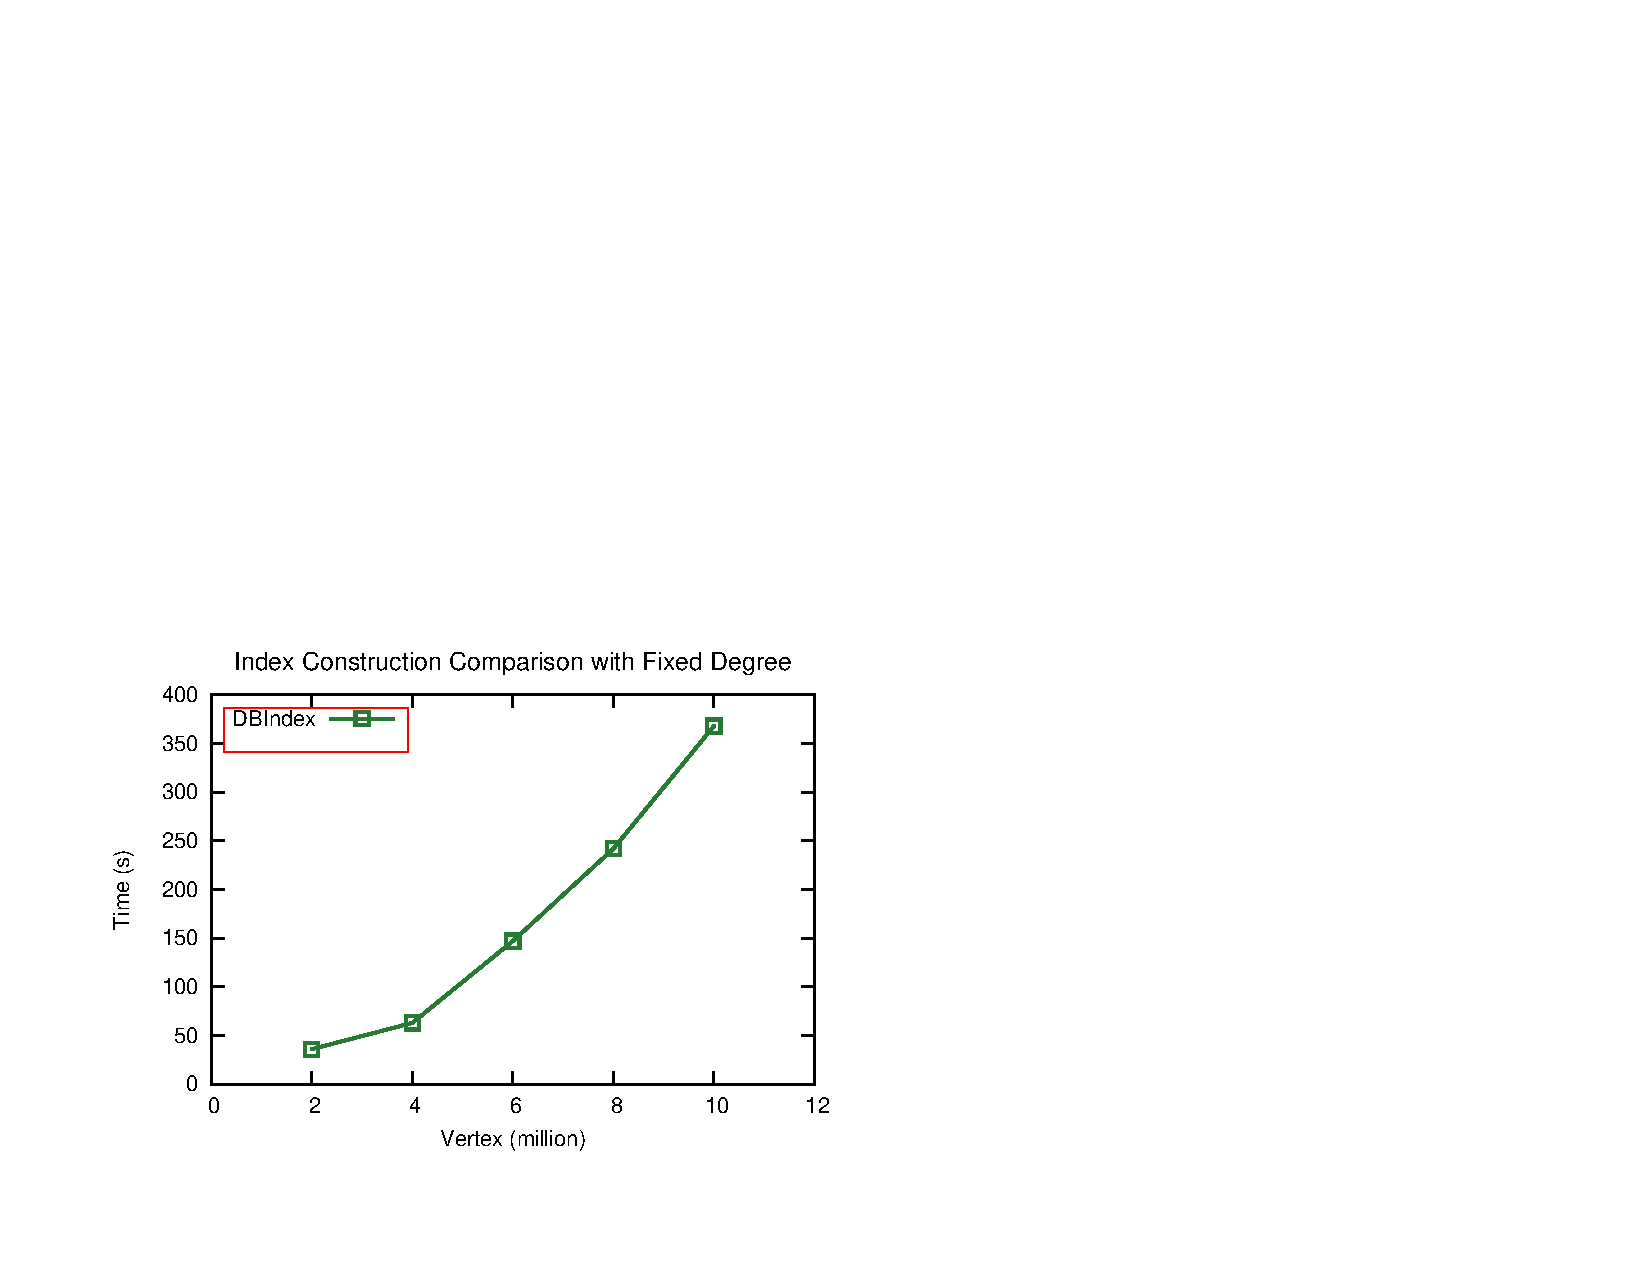
\includegraphics[width=\textwidth]{chapter3/exp/khopeffect/scalability/d10h2_query.pdf}
  \caption{2-hop query performance}
\end{subfigure}
\caption{Impact of number of vertexes.}
\label{fig:khop_d10_h1}
\end{figure}

\begin{figure}[t]
\centering
\begin{subfigure}{0.45\linewidth}
  \centering
  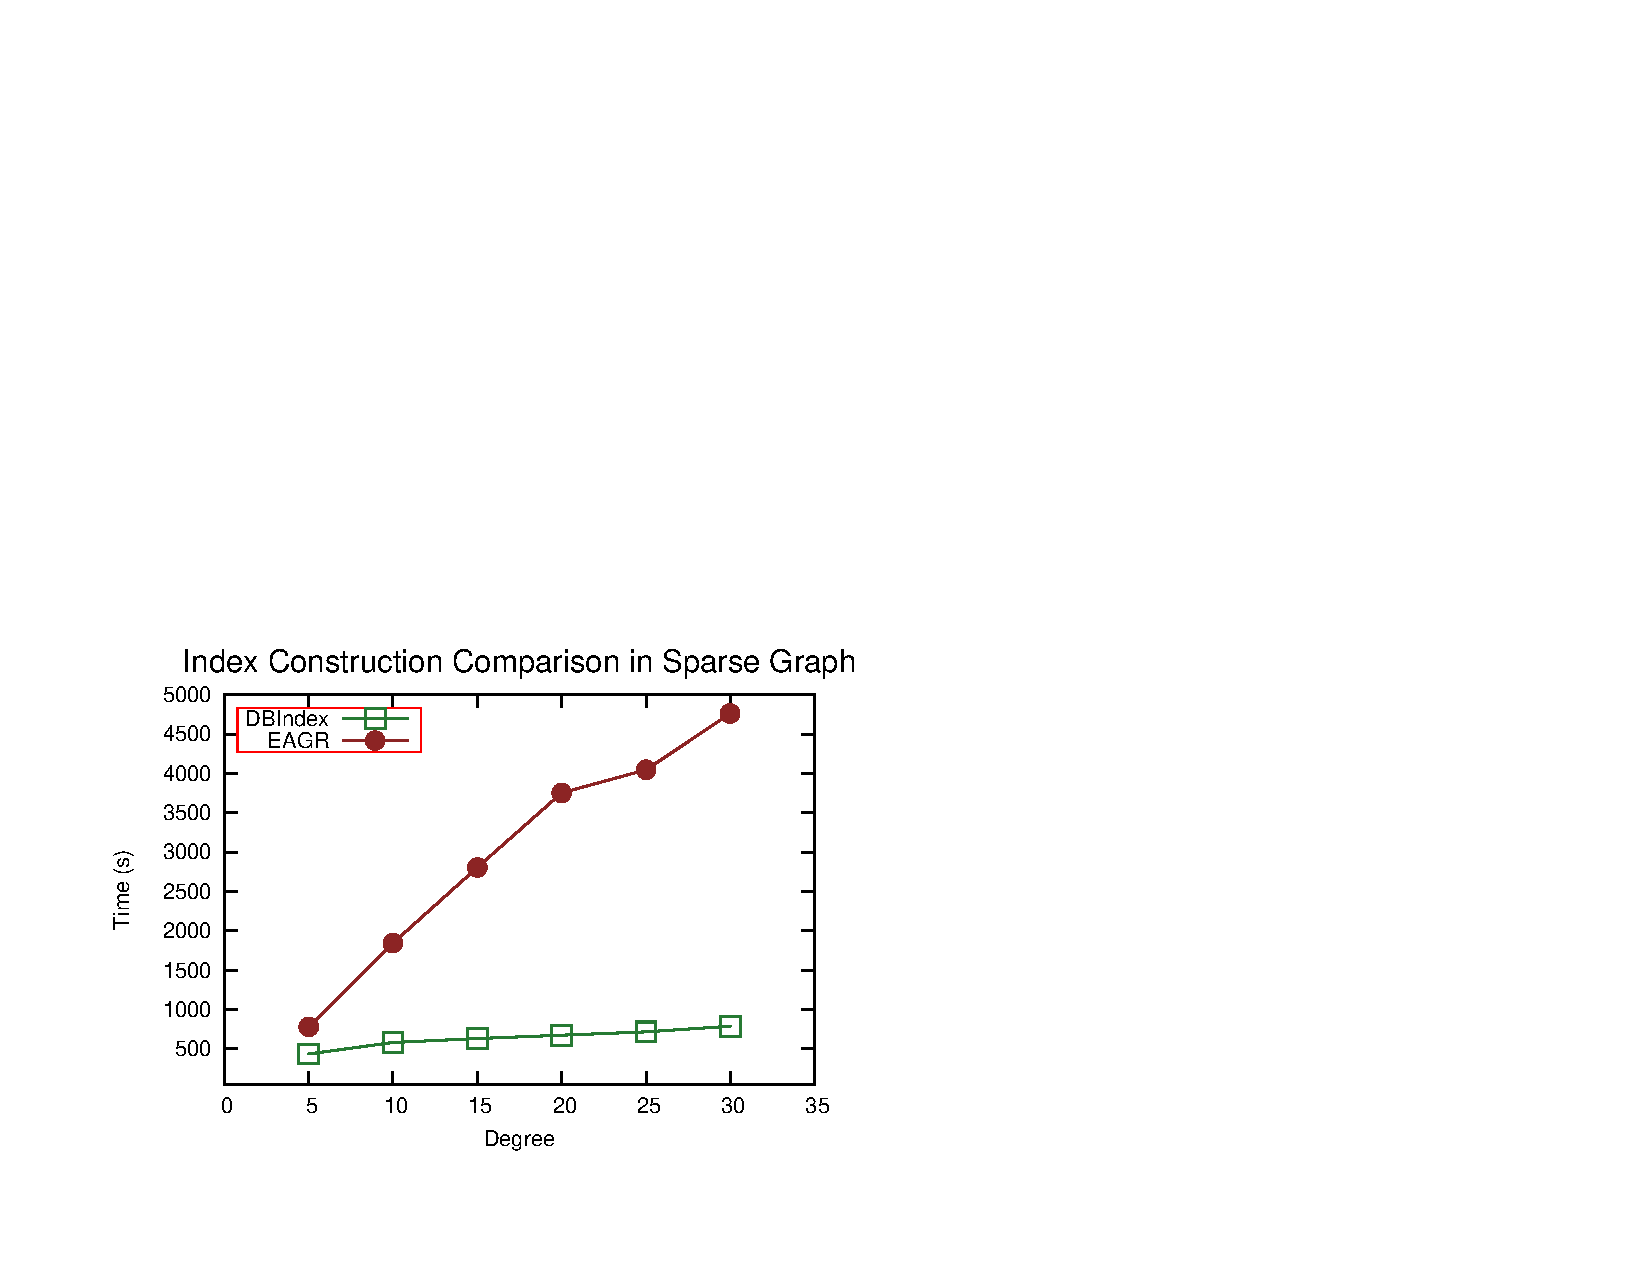
\includegraphics[width=\textwidth]{chapter3/exp/khopeffect/scalability/varyd_index_2M.pdf}
  \caption{1-hop index construction}
\end{subfigure}
\begin{subfigure}{0.45\linewidth}
  \centering
  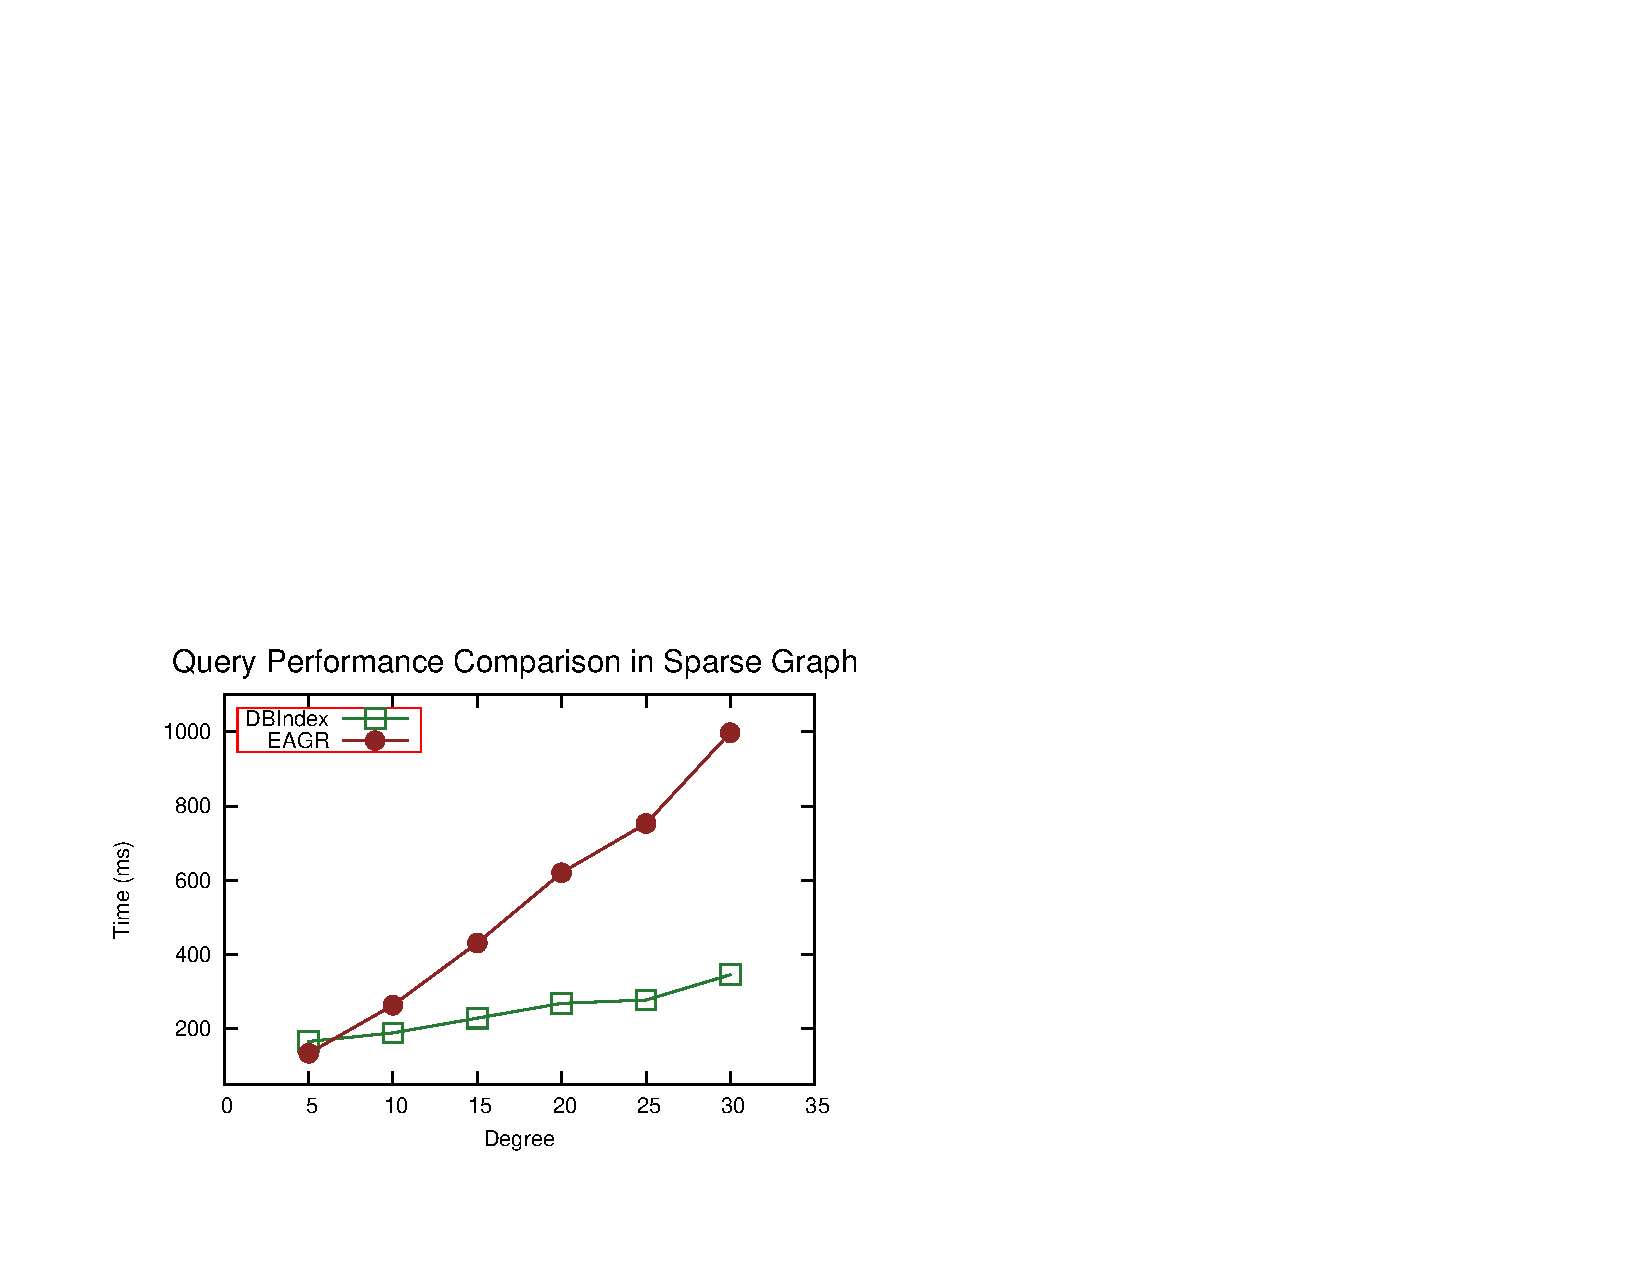
\includegraphics[width=\textwidth]{chapter3/exp/khopeffect/scalability/varyd_query_2M.pdf}
  \caption{1-hop query performance}
\end{subfigure}
\begin{subfigure}{0.45\linewidth}
  \centering
  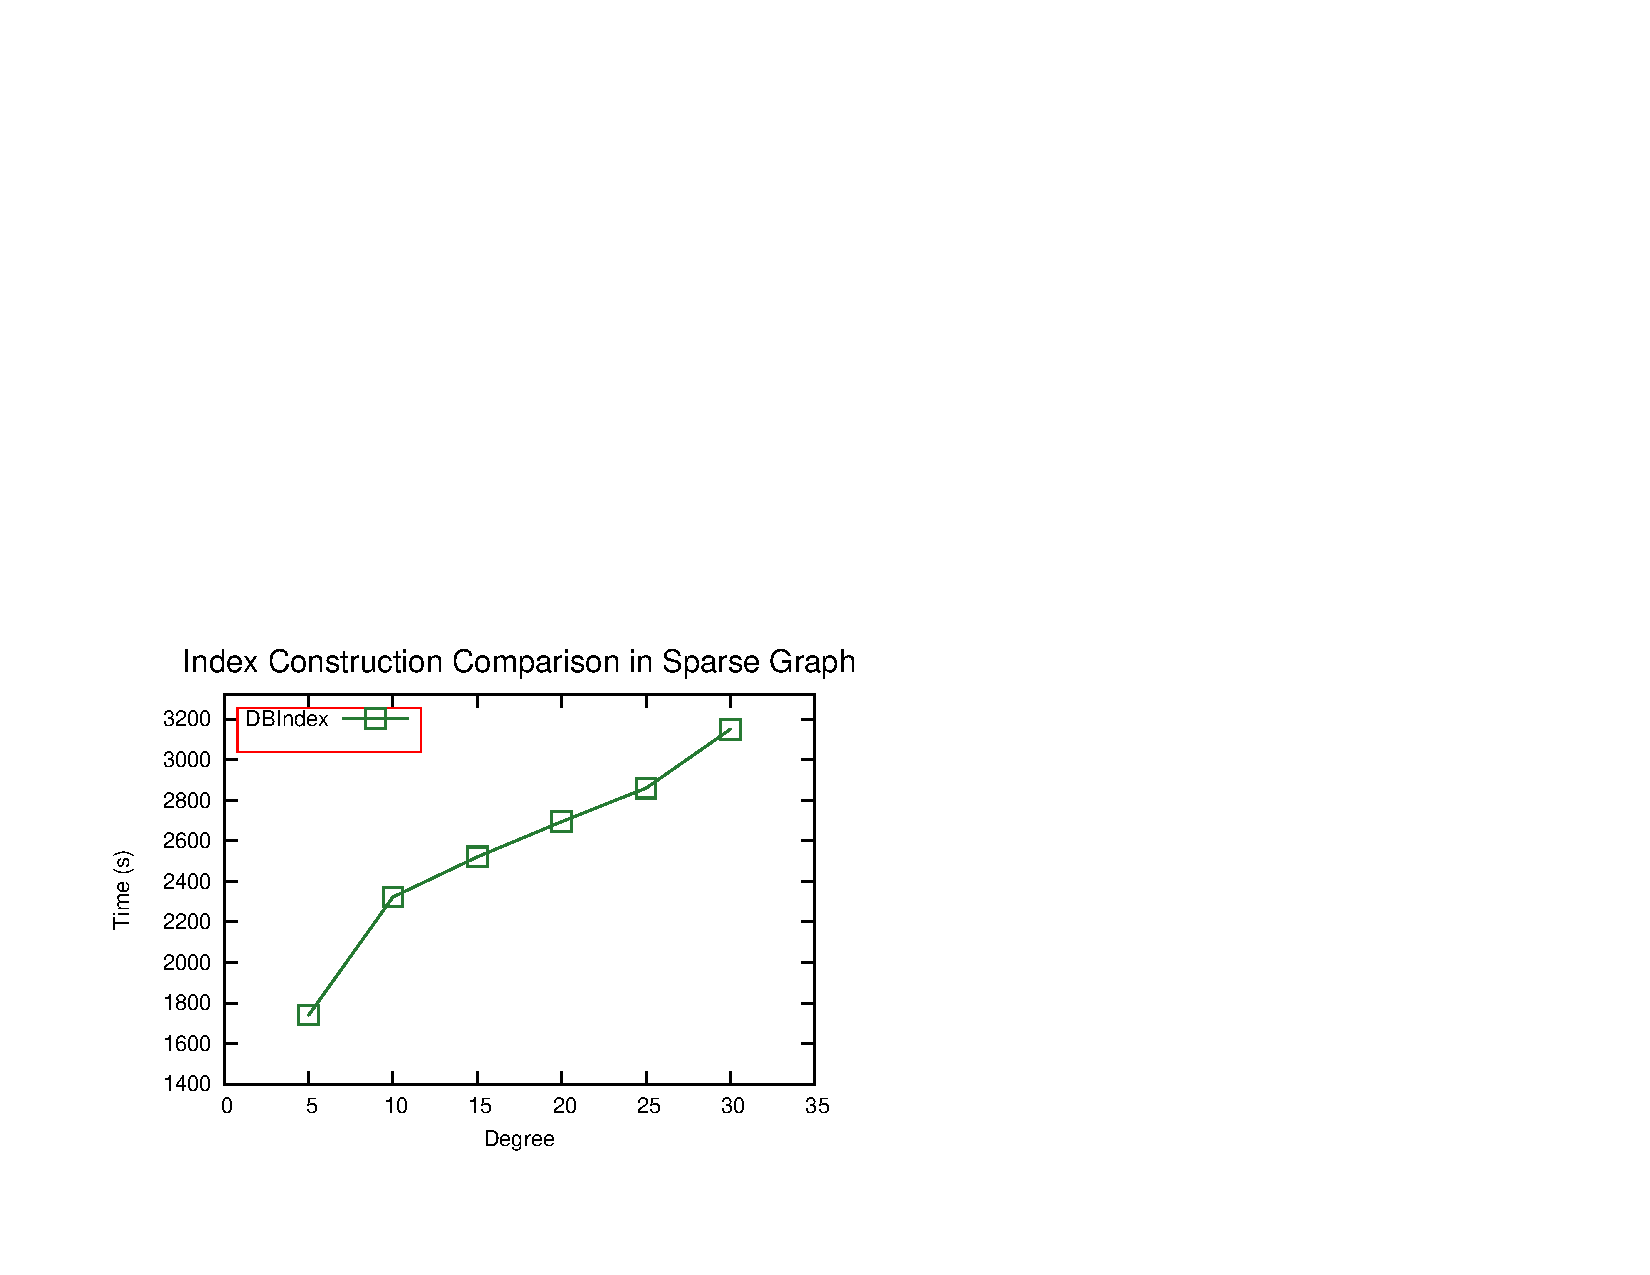
\includegraphics[width=\textwidth]{chapter3/exp/khopeffect/scalability/varyd_index_2M_h2.pdf}
  \caption{2-hop index construction}
\end{subfigure}
\begin{subfigure}{0.45\linewidth}
  \centering
  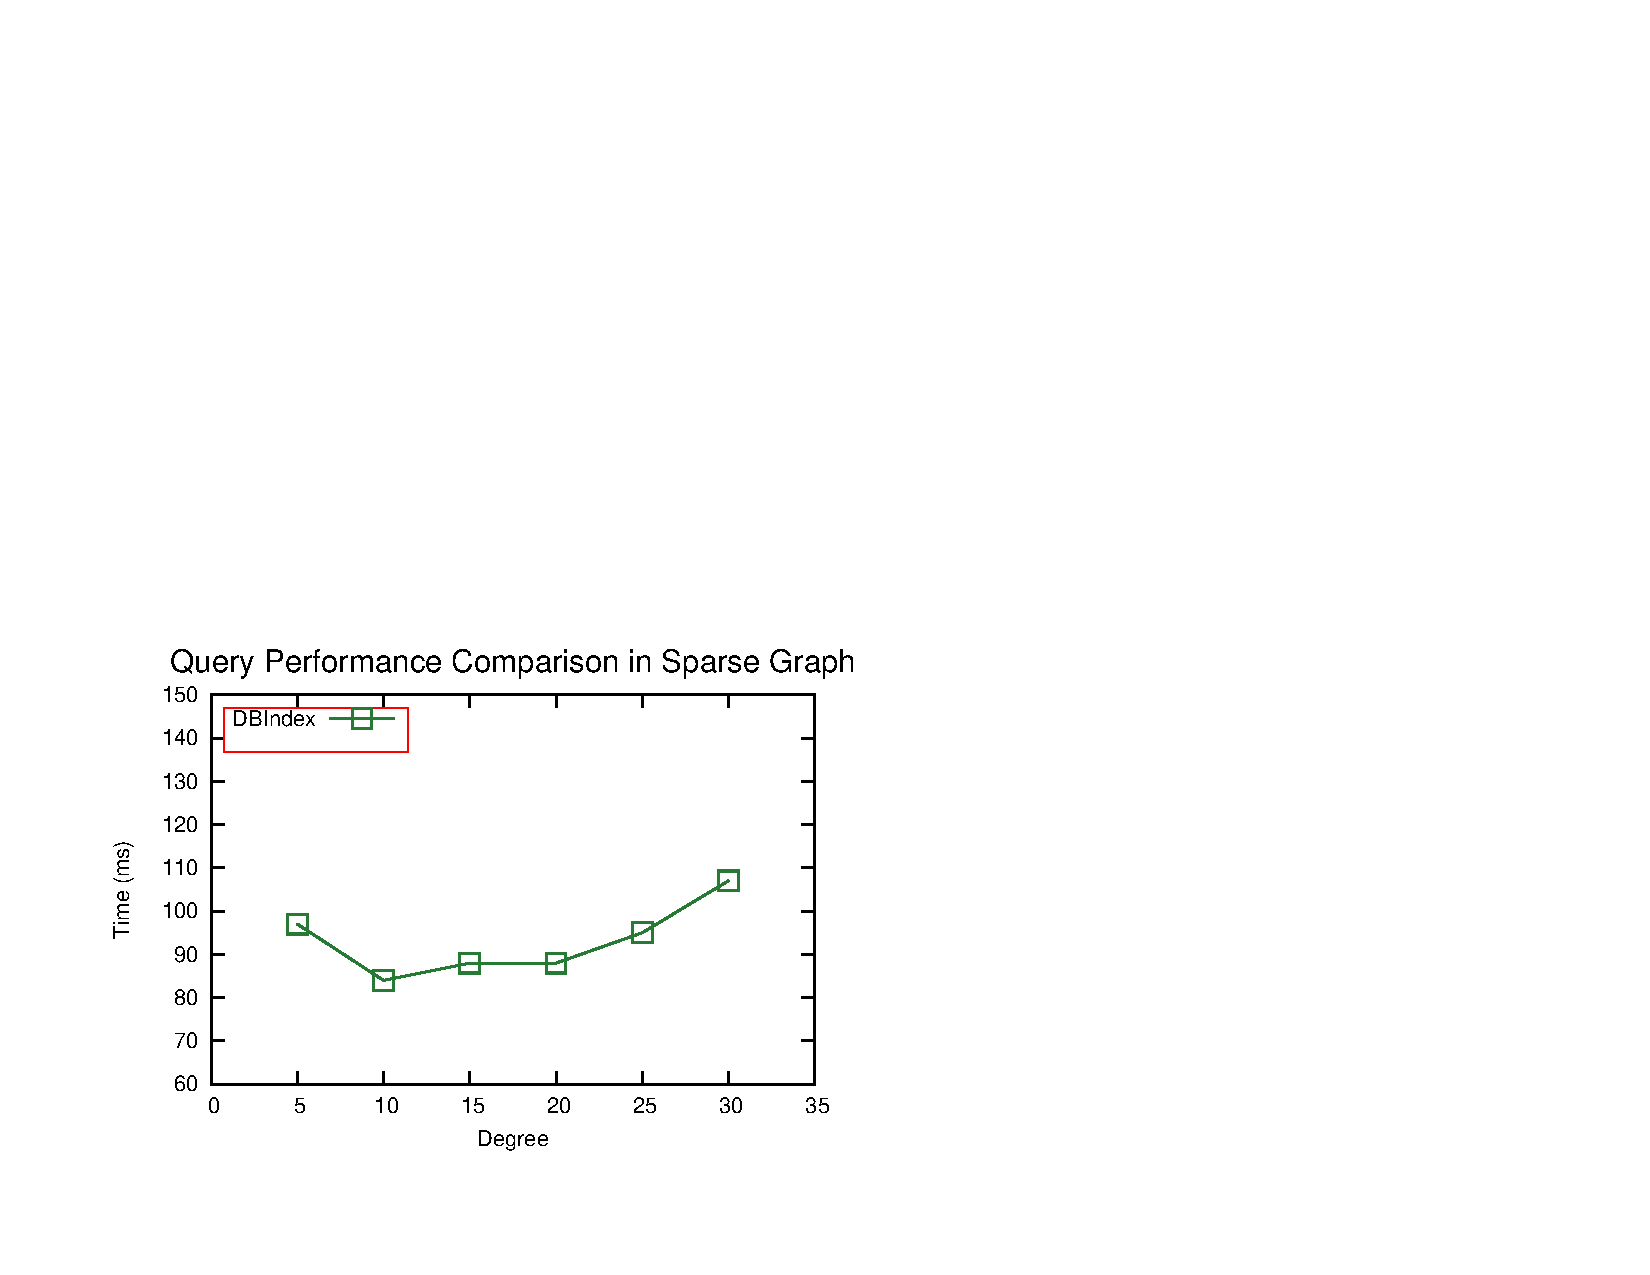
\includegraphics[width=\textwidth]{chapter3/exp/khopeffect/scalability/varyd_query_2M_h2.pdf}
  \caption{2-hop query performance}
\end{subfigure}
\caption{Impact of degree in sparse graphs with 2M vertexes.}
\label{fig:khop_v2m}
\end{figure}

\textbf{Impact of Sparse Graphs.} Our proposed DBIndex is effective when there is significant overlap between windows of neighboring nodes. As such, it is interesting to study how it performs for sparse graph where the vertexes may not share many common neighbors. In these experiments, 
we study the impact of degree when the graph is relatively sparse.
We fix the number vertexes of 2M and vary the vertex degree from 5 to 30. 
Figures~\ref{fig:khop_v2m} (a) and (c) present the results 
on index construction for the 1-hop and the 2-hop queries respectively. 
For the 1-hop query, as degree increases, the time for index
construction also increases. 
However, the index creation time of DBIndex increases much 
slower than EAGR. This is because EAGR incurs relatively more 
overhead to handle multiple FP-Tree creation and reconstruction. 
For the 2-hop query, EAGR again fails to run due to the memory limitation. %This is because even for a very sparse graph (i.e., degree 5), the initial vertex-mapping can be as large 
%as 90GB in a linked list representation, which exceeds the available memory. 
%Note that the size becomes even larger when it is stored in the matrix form.
Therefore, we only show the results of DBIndex. 
In Figure~\ref{fig:khop_v2m} (c), the index construction time of DBIndex increases as the 
degree increases. This is expected as a bigger degree  
increases the overhead of graph traversal time to collect the window. 


Figures~\ref{fig:khop_v2m} (b) and (d)
show the results on query time 
for 1-hop and 2-hop queries respectively. 
We observe a similar pattern for the index construction time:
for the 1-hop query, the query time increases with increasing degree
but at a much slower rate than EAGR; For the 2-hop query, we observe in Figure~\ref{fig:khop_v2m} (d) that the
query performance of DBIndex hovers around 100ms, which is much 
smaller than that of the 1-hop query performance. 
This is because there are more dense blocks in the 2-hop case, 
in which case the query time can be faster compared to the 1-hop case. 

\textbf{Impact of Dense Graphs.} We study the 
impact of degree over very dense graphs with 200k vertexes 
when the degree changes from 80 to 200. 
Figures~\ref{fig:khop_v200k} (a) and (c) show
the execution time for index construction 
for 1-hop and 2-hop queries respectively. From the results, 
we can see that DBIndex also performs well on dense graphs. 
As the degree increases, EAGR's performance degrades much faster than DBIndex. For the 2-hop query,
as shown in Figures~\ref{fig:khop_v200k} (b) and (d), EAGR is only able to work on 
the dataset with degree 80 due to the memory issue. 
Even though the number of vertexes is relatively small (only 200k), 
the number of edges is very large when the degree becomes big 
(e.g. 40M edges with degree of 200). 
%
Figures~\ref{fig:khop_v200k} 
(b) and (d) show the results on query performance 
for the 1-hop and the 2-hop queries respectively. 
The results are consistent with that for sparse graphs: DBIndex is superior over EAGR. 

In summary, the insight we obtained is that the scalability of EAGR 
is highly limited by its large usage of memory.
%: the graph size and the number of hops. 
DBIndex achieves better scalability as it does not need to 
create a large amount of intermediate data in memory. 

\begin{figure}[h]
\centering
\begin{subfigure}{0.45\linewidth}
  \centering
  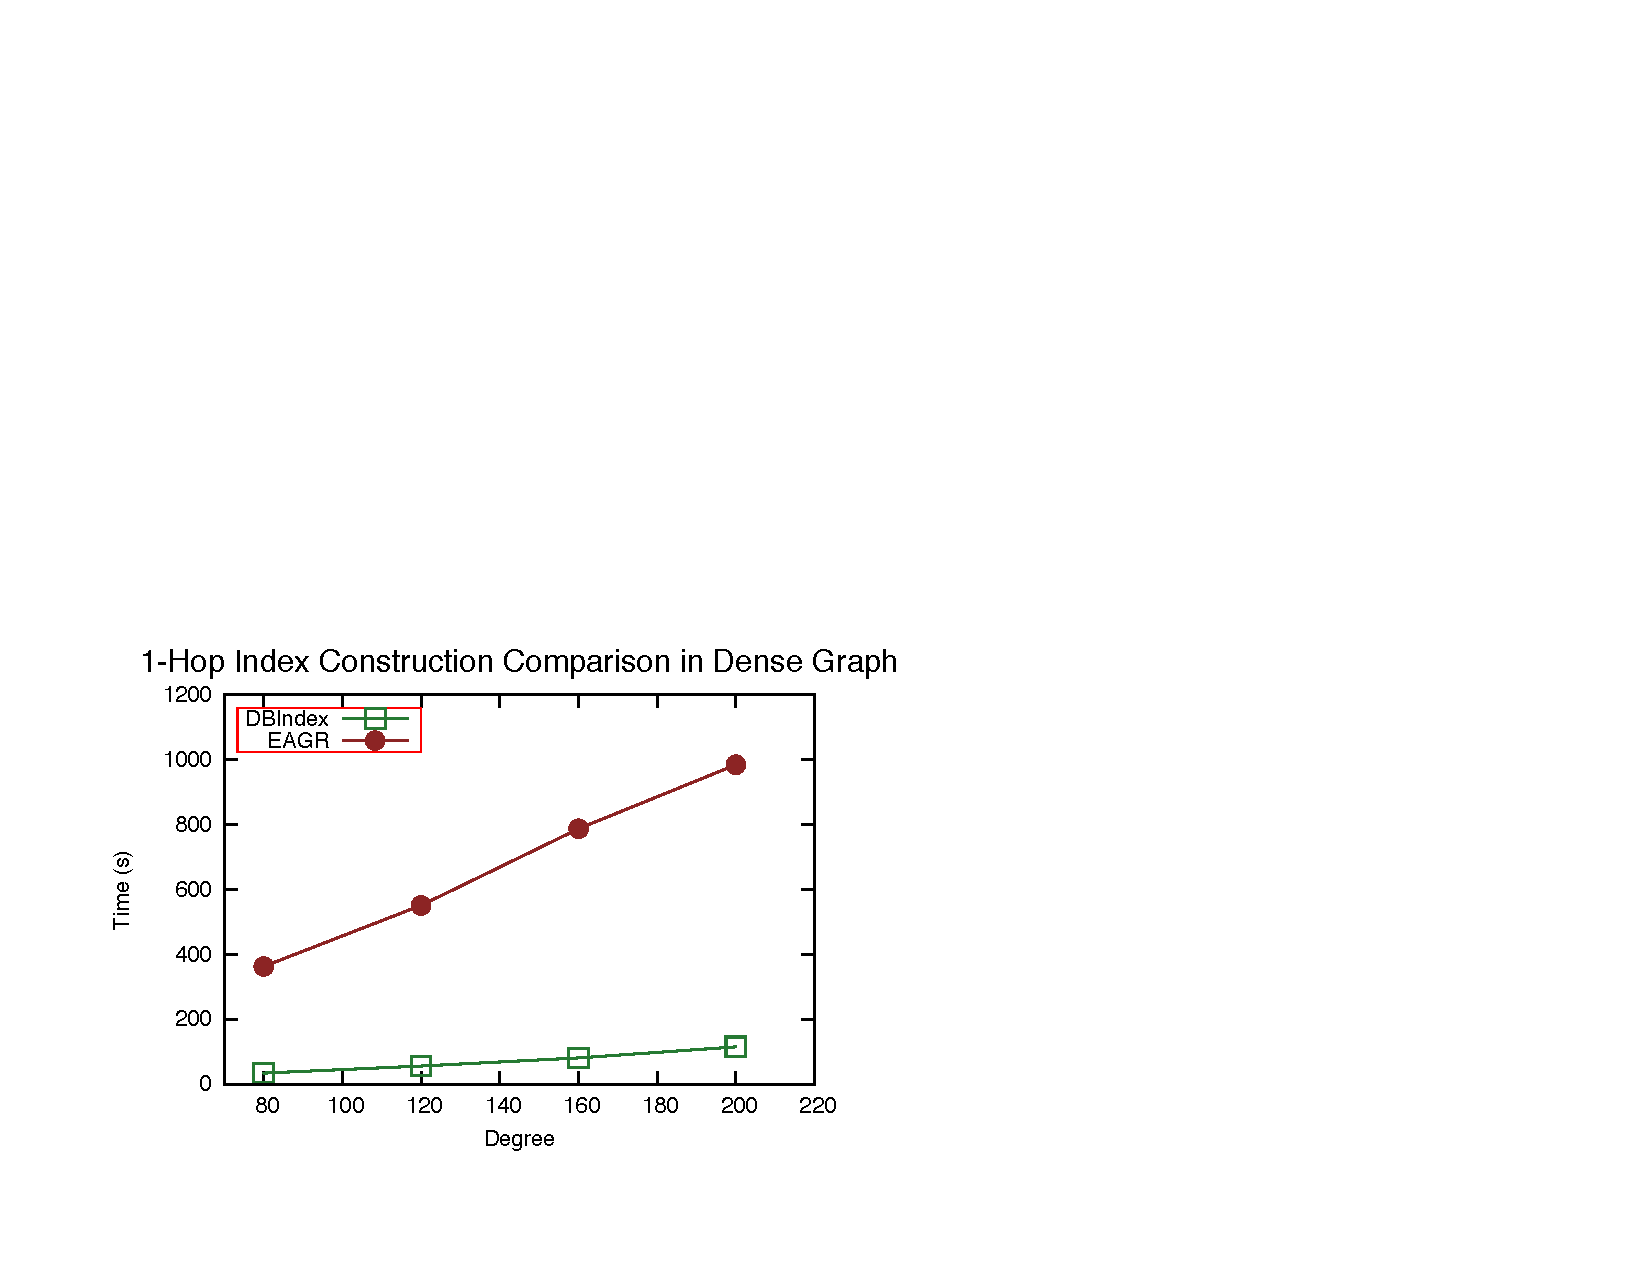
\includegraphics[width=\textwidth]{chapter3/exp/khopeffect/scalability/varyd_index_200k.pdf}
  \caption{1-hop index construction}
\end{subfigure}
\begin{subfigure}{0.45\linewidth}
  \centering
  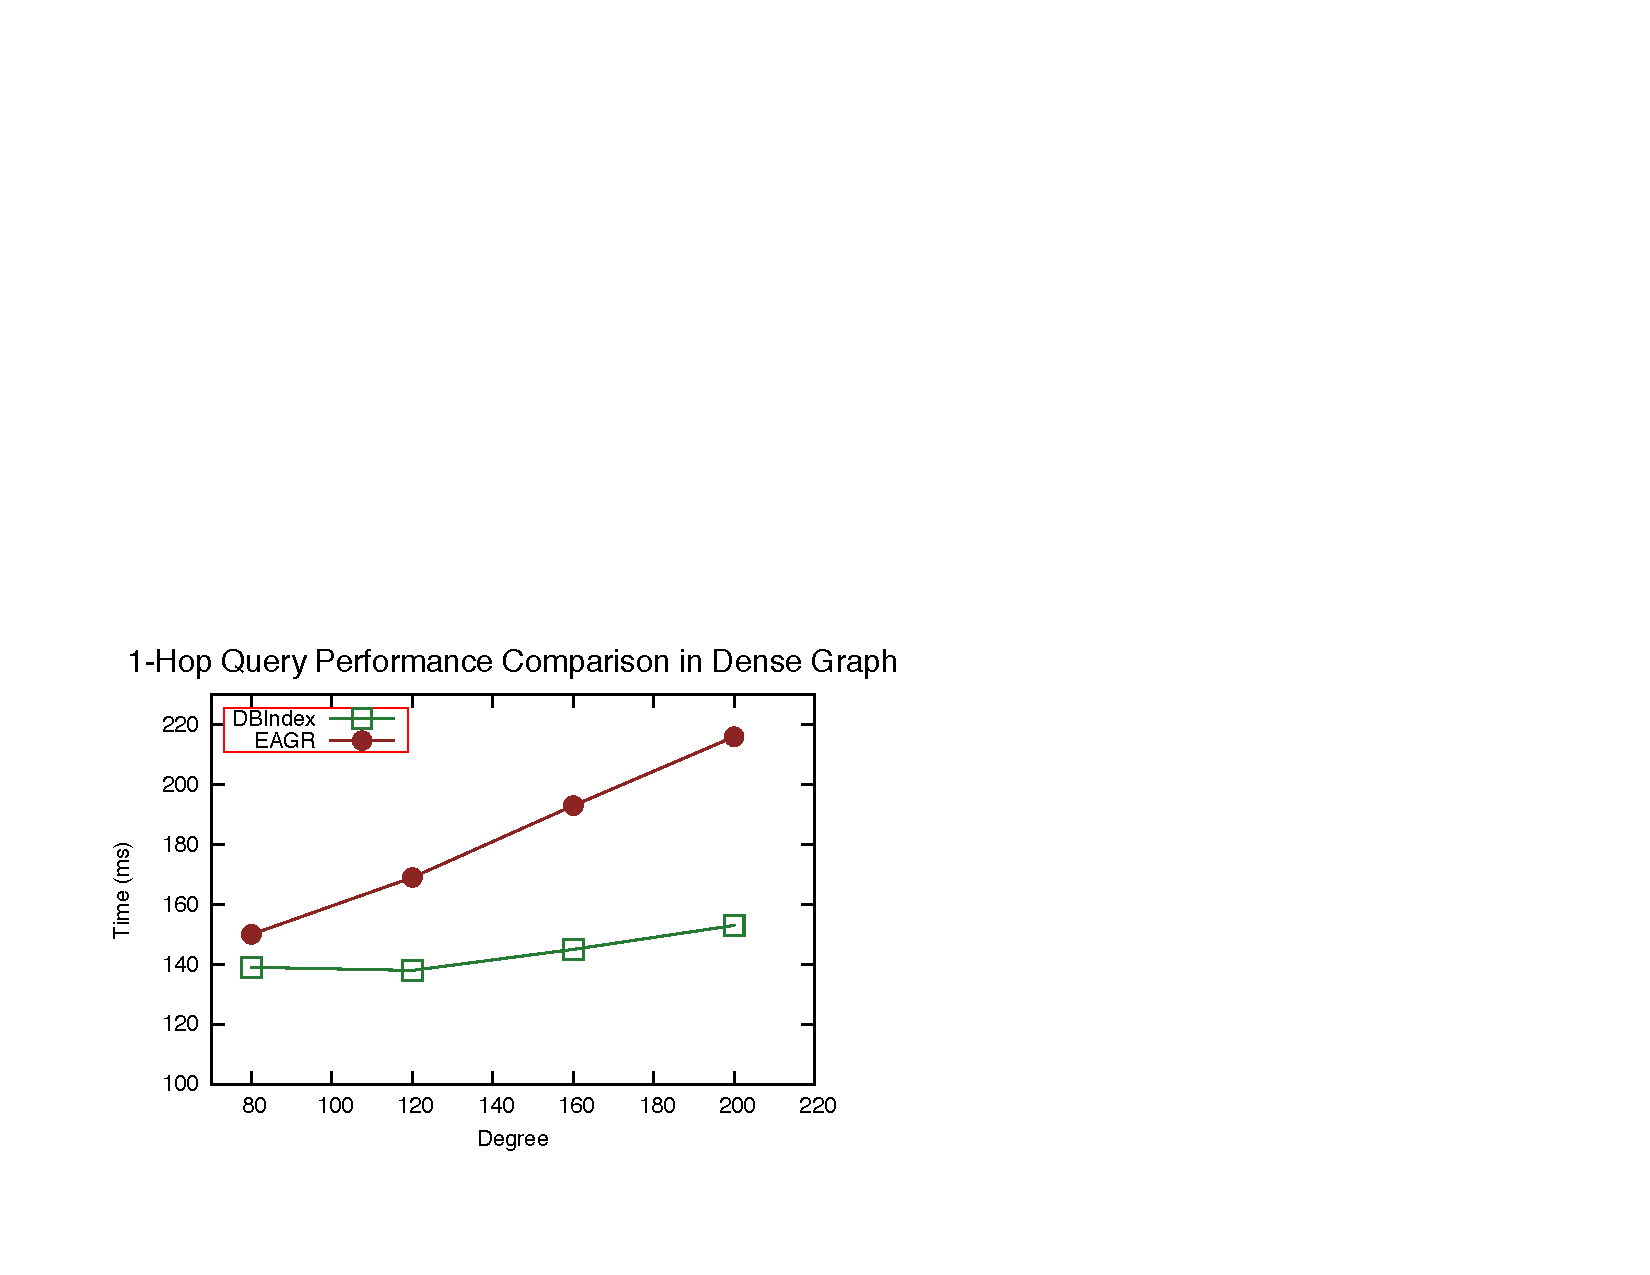
\includegraphics[width=\textwidth]{chapter3/exp/khopeffect/scalability/varyd_query_200k.pdf}
  \caption{1-hop query performance}
\end{subfigure}
\begin{subfigure}{0.45\linewidth}
  \centering
  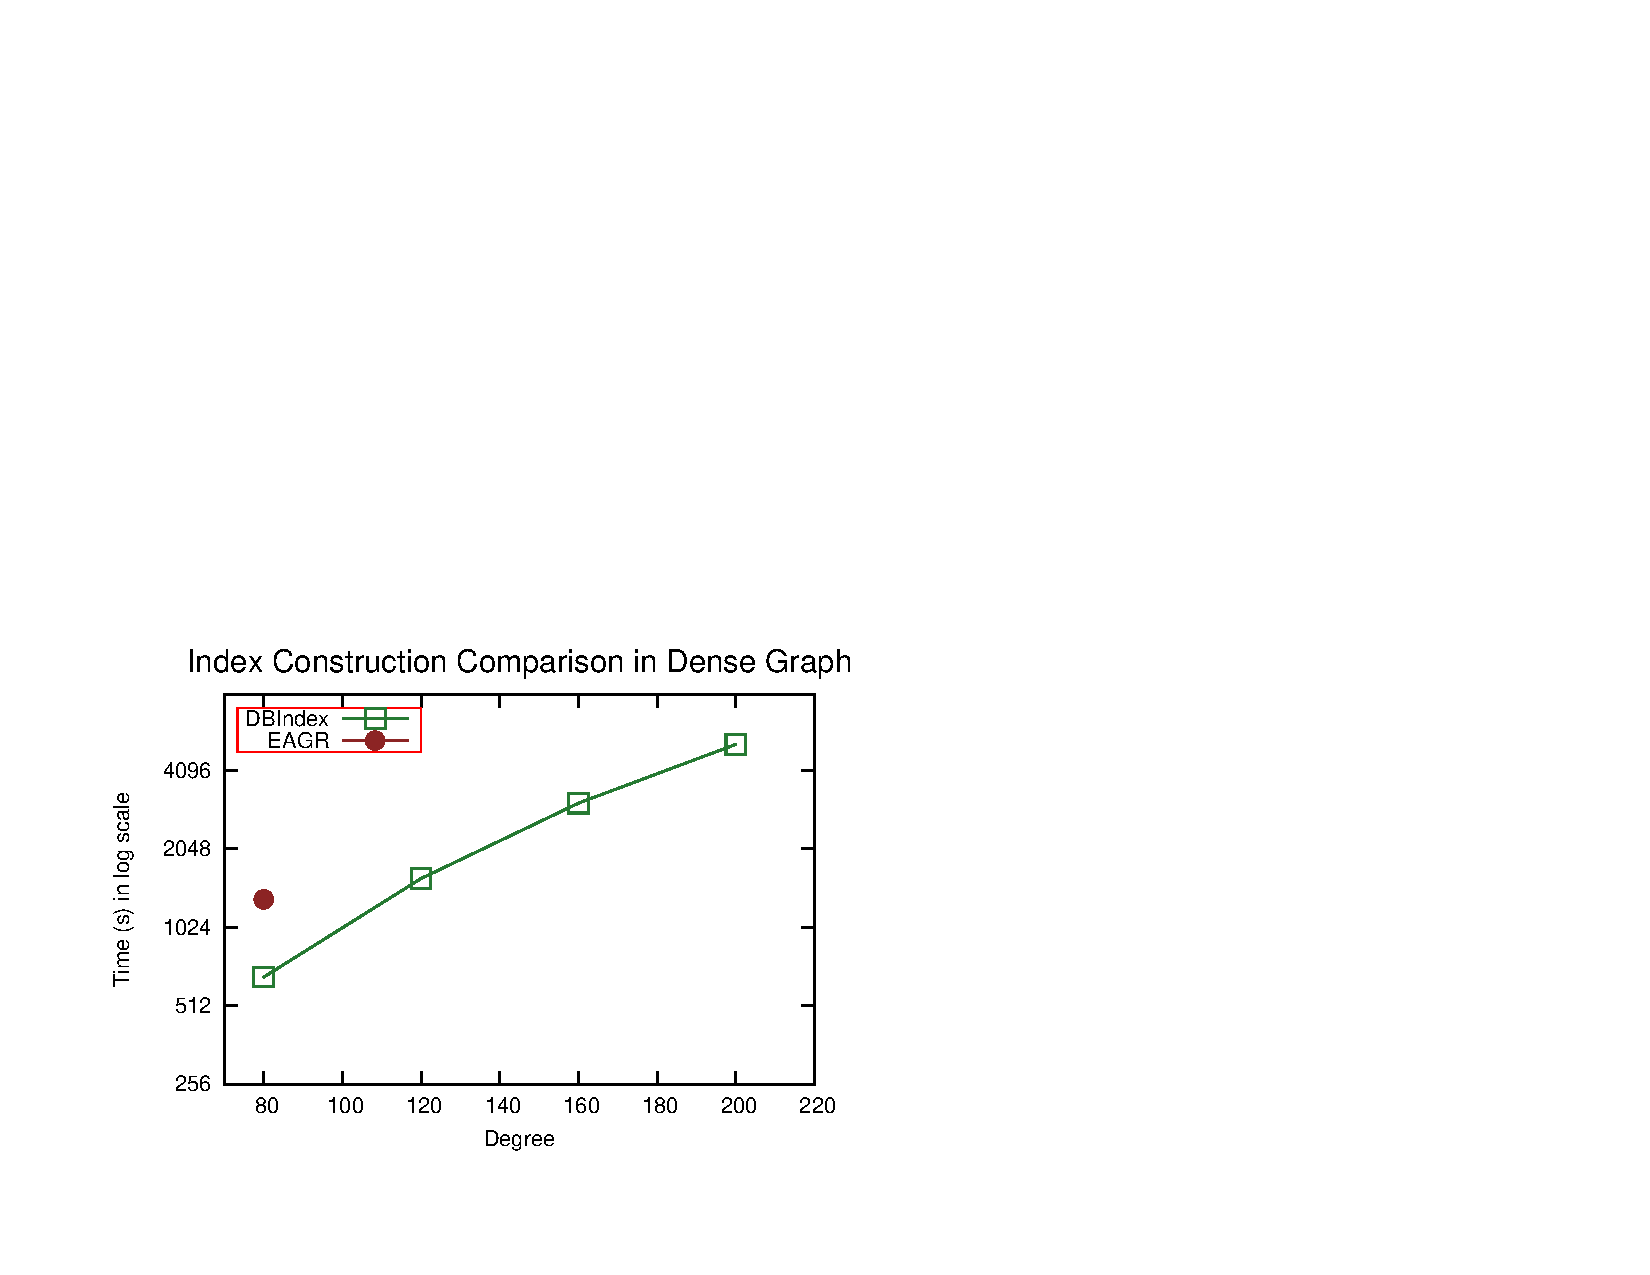
\includegraphics[width=\textwidth]{chapter3/exp/khopeffect/scalability/varyd_index_200k_h2.pdf}
  \caption{2-hop index construction}
\end{subfigure}
\begin{subfigure}{0.45\linewidth}
  \centering
  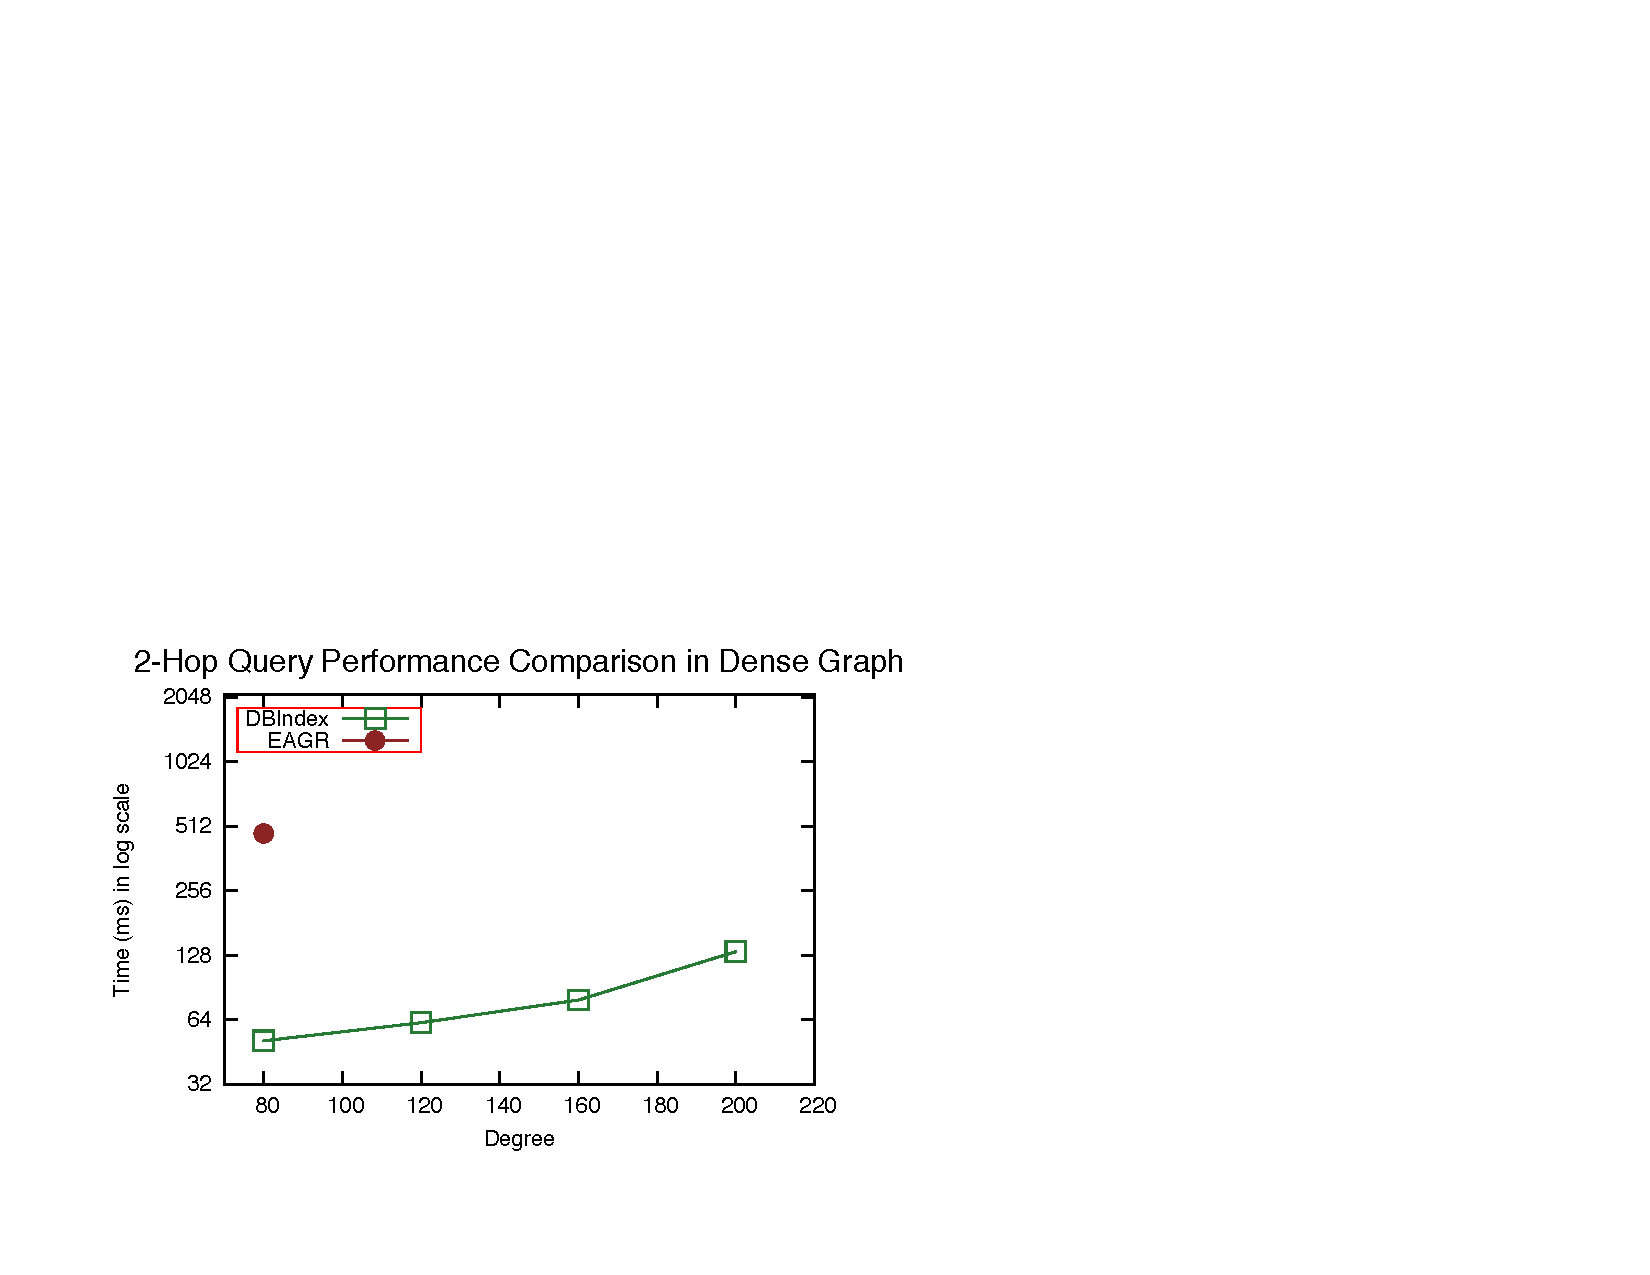
\includegraphics[width=\textwidth]{chapter3/exp/khopeffect/scalability/varyd_query_200k_h2.pdf}
  \caption{2-hop query performance }
\end{subfigure}
\caption{Impact of degree in dense graphs with 200K vertexes.}
\label{fig:khop_v200k}
\end{figure}

\subsection{Evaluation of I-Index}
In this set of experiments, we evaluate I-Index. 
All the datasets are generated from the DAGGER generator.   

\begin{figure}[h]
\centering
\begin{subfigure}{0.45\linewidth}
  \centering
  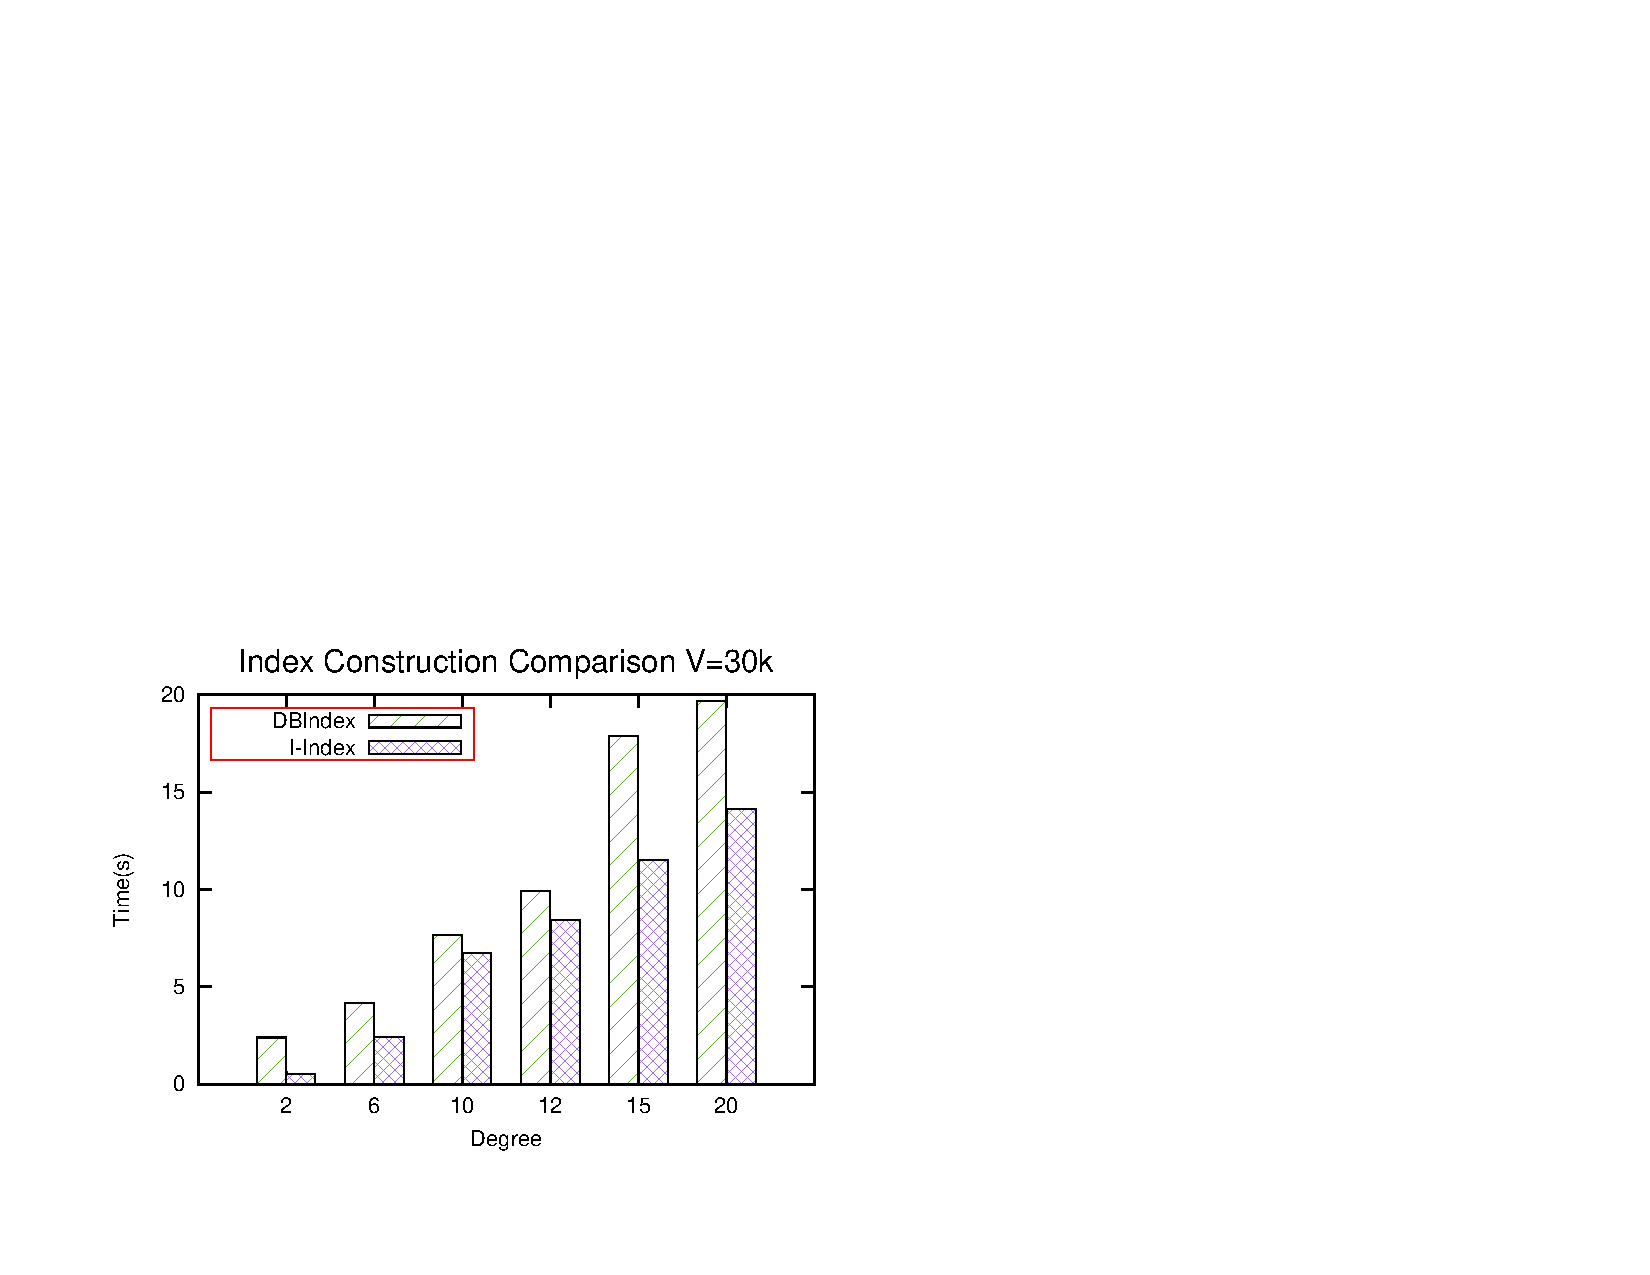
\includegraphics[width=\textwidth]{chapter3/exp/topoeffect/comp/top_index_time_v30k.pdf}
  \caption{Index construction}
\end{subfigure}
\begin{subfigure}{0.45\linewidth}
  \centering
  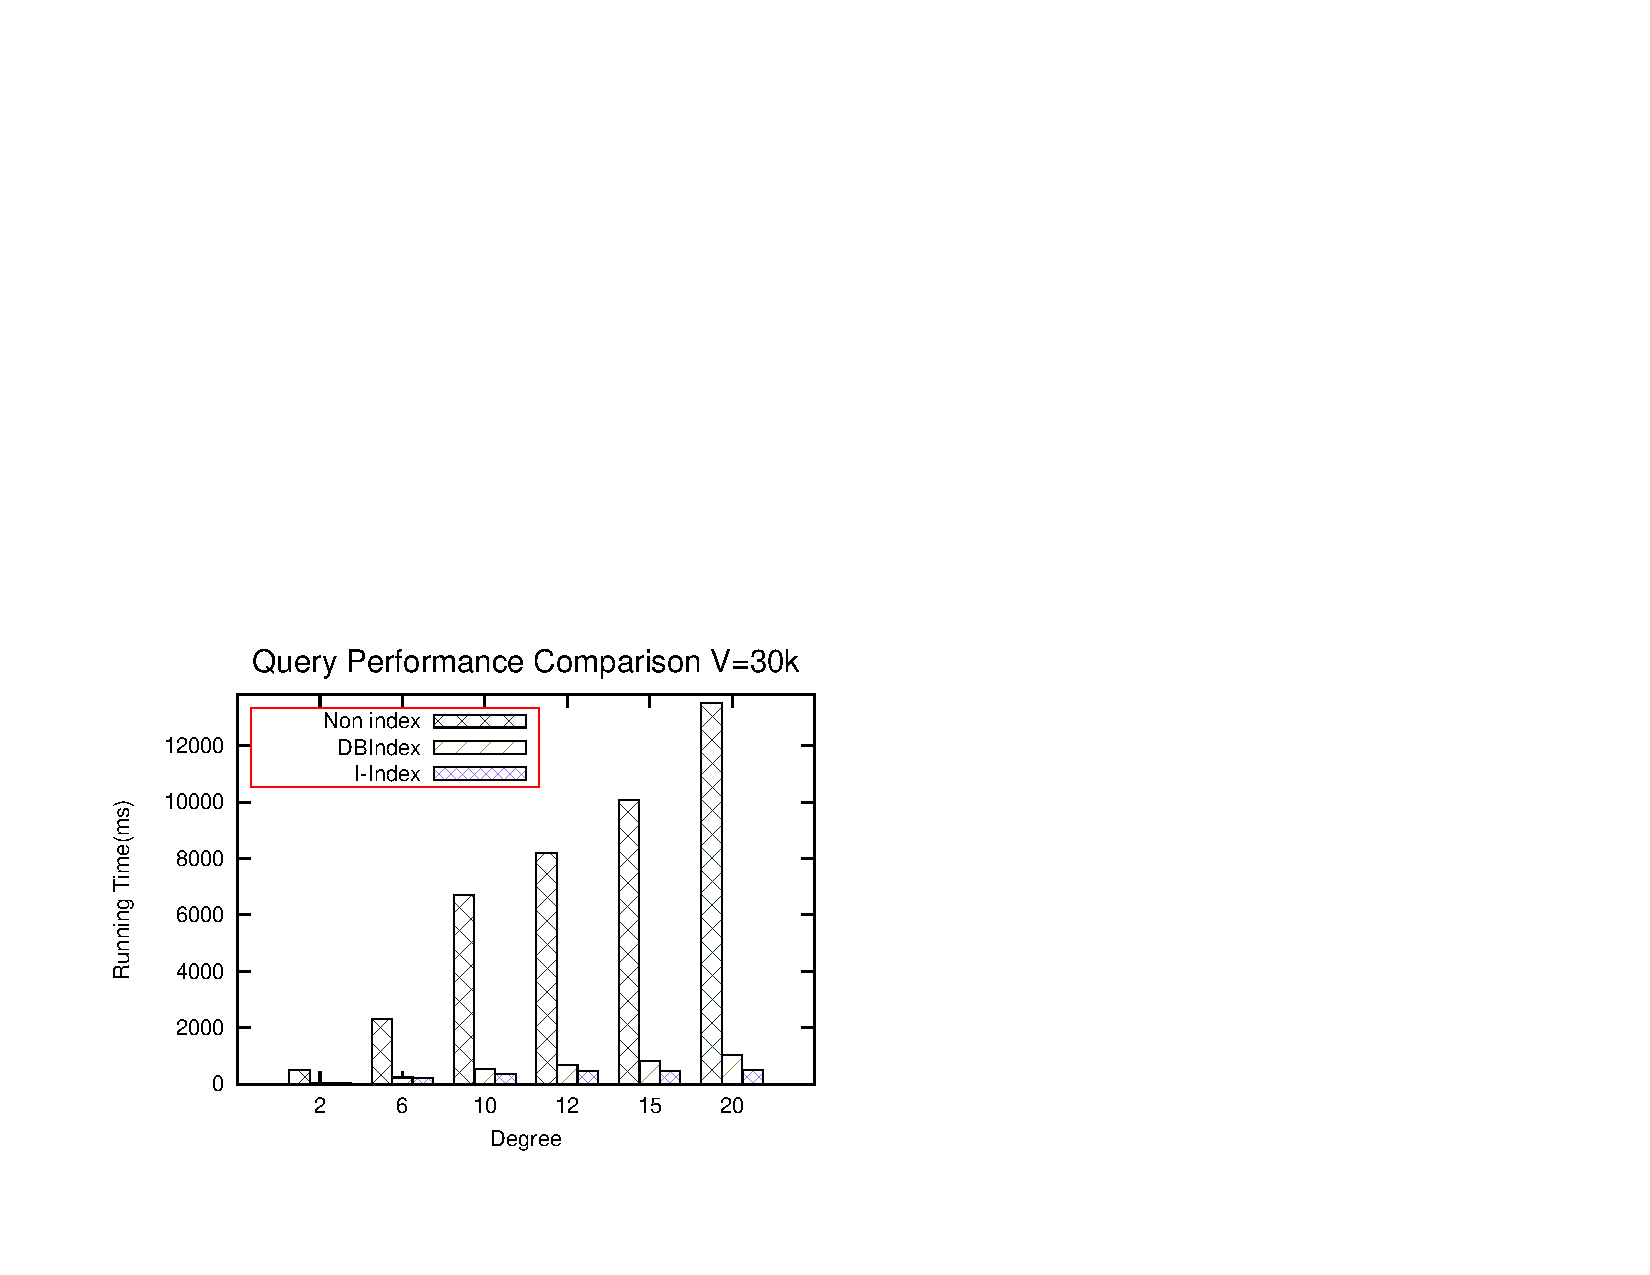
\includegraphics[width=\textwidth]{chapter3/exp/topoeffect/comp/top_query_time_v30k.pdf}
  \caption{Query performance}
\end{subfigure}
\begin{subfigure}{0.45\linewidth}
  \centering
  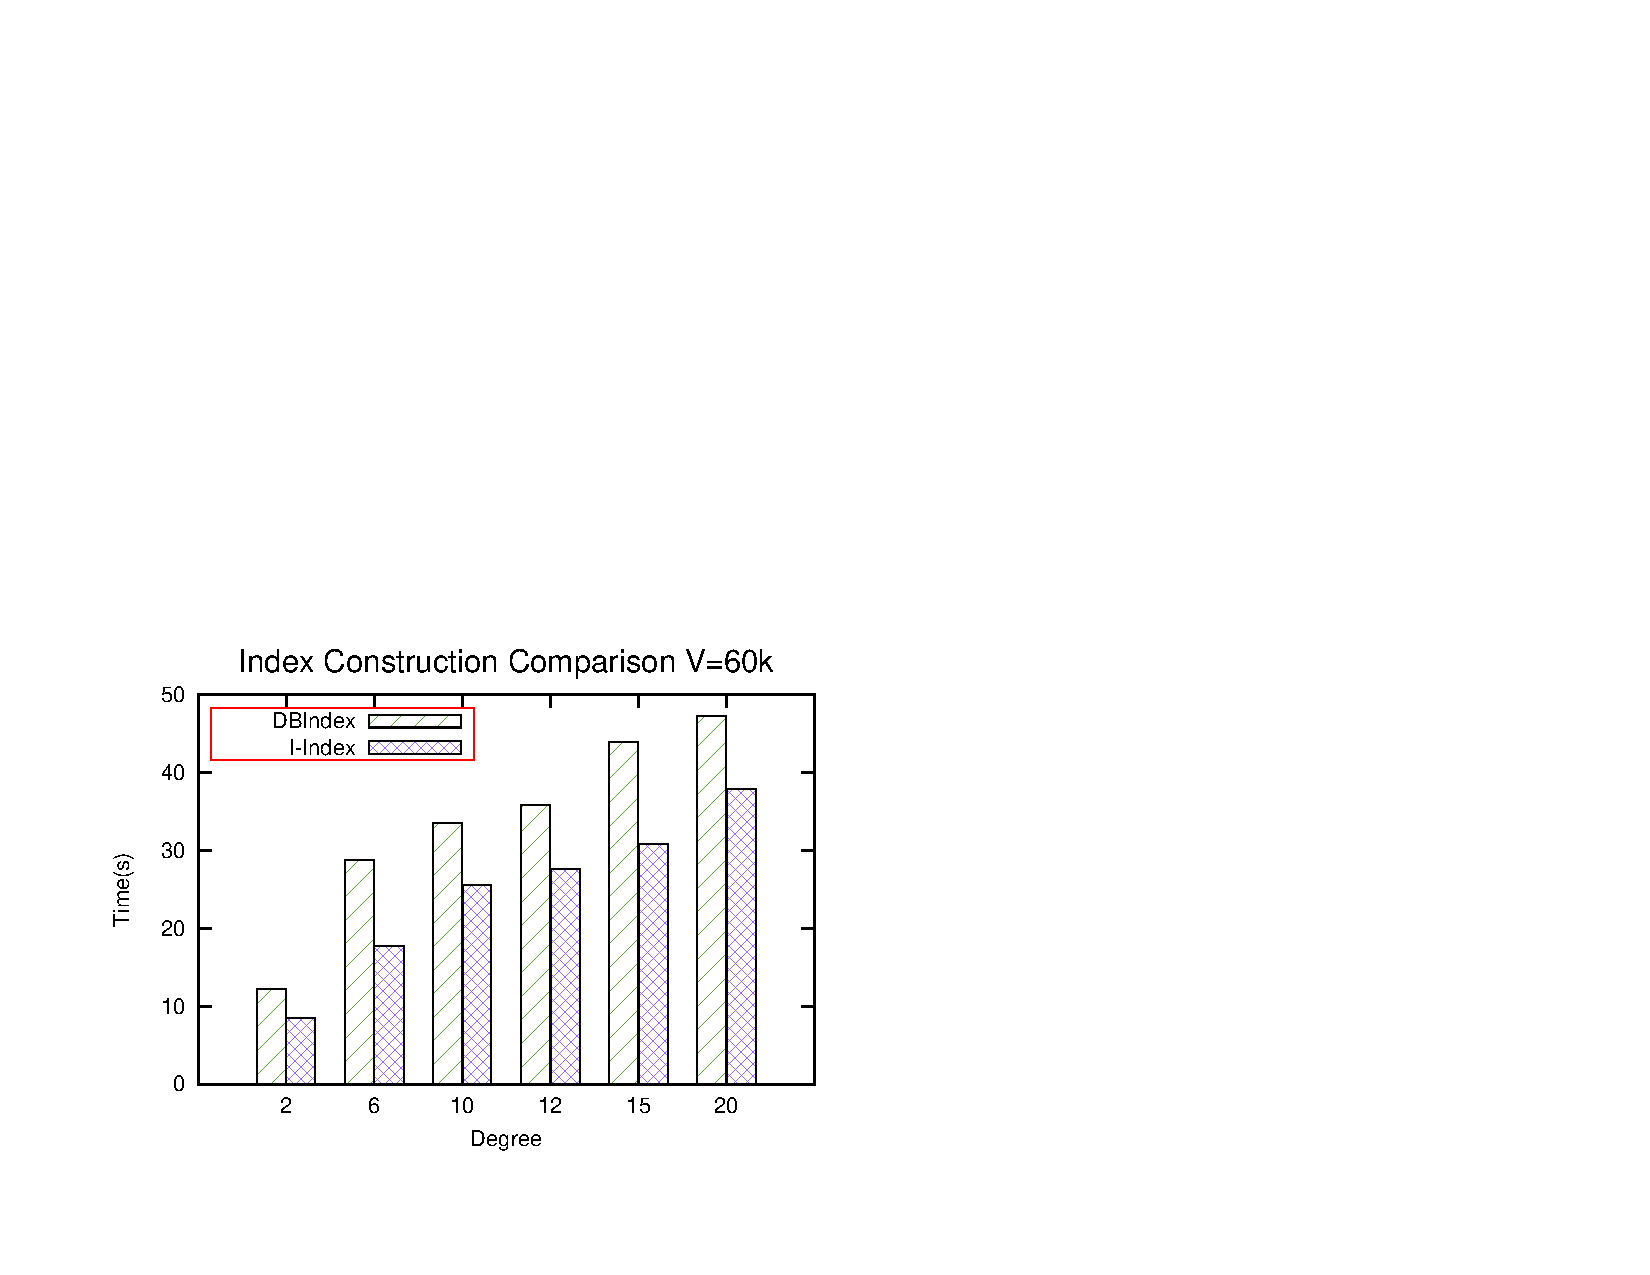
\includegraphics[width=\textwidth]{chapter3/exp/topoeffect/comp/top_index_time_v60k.pdf}
  \caption{Index construction}
\end{subfigure}
\begin{subfigure}{0.45\linewidth}
  \centering
  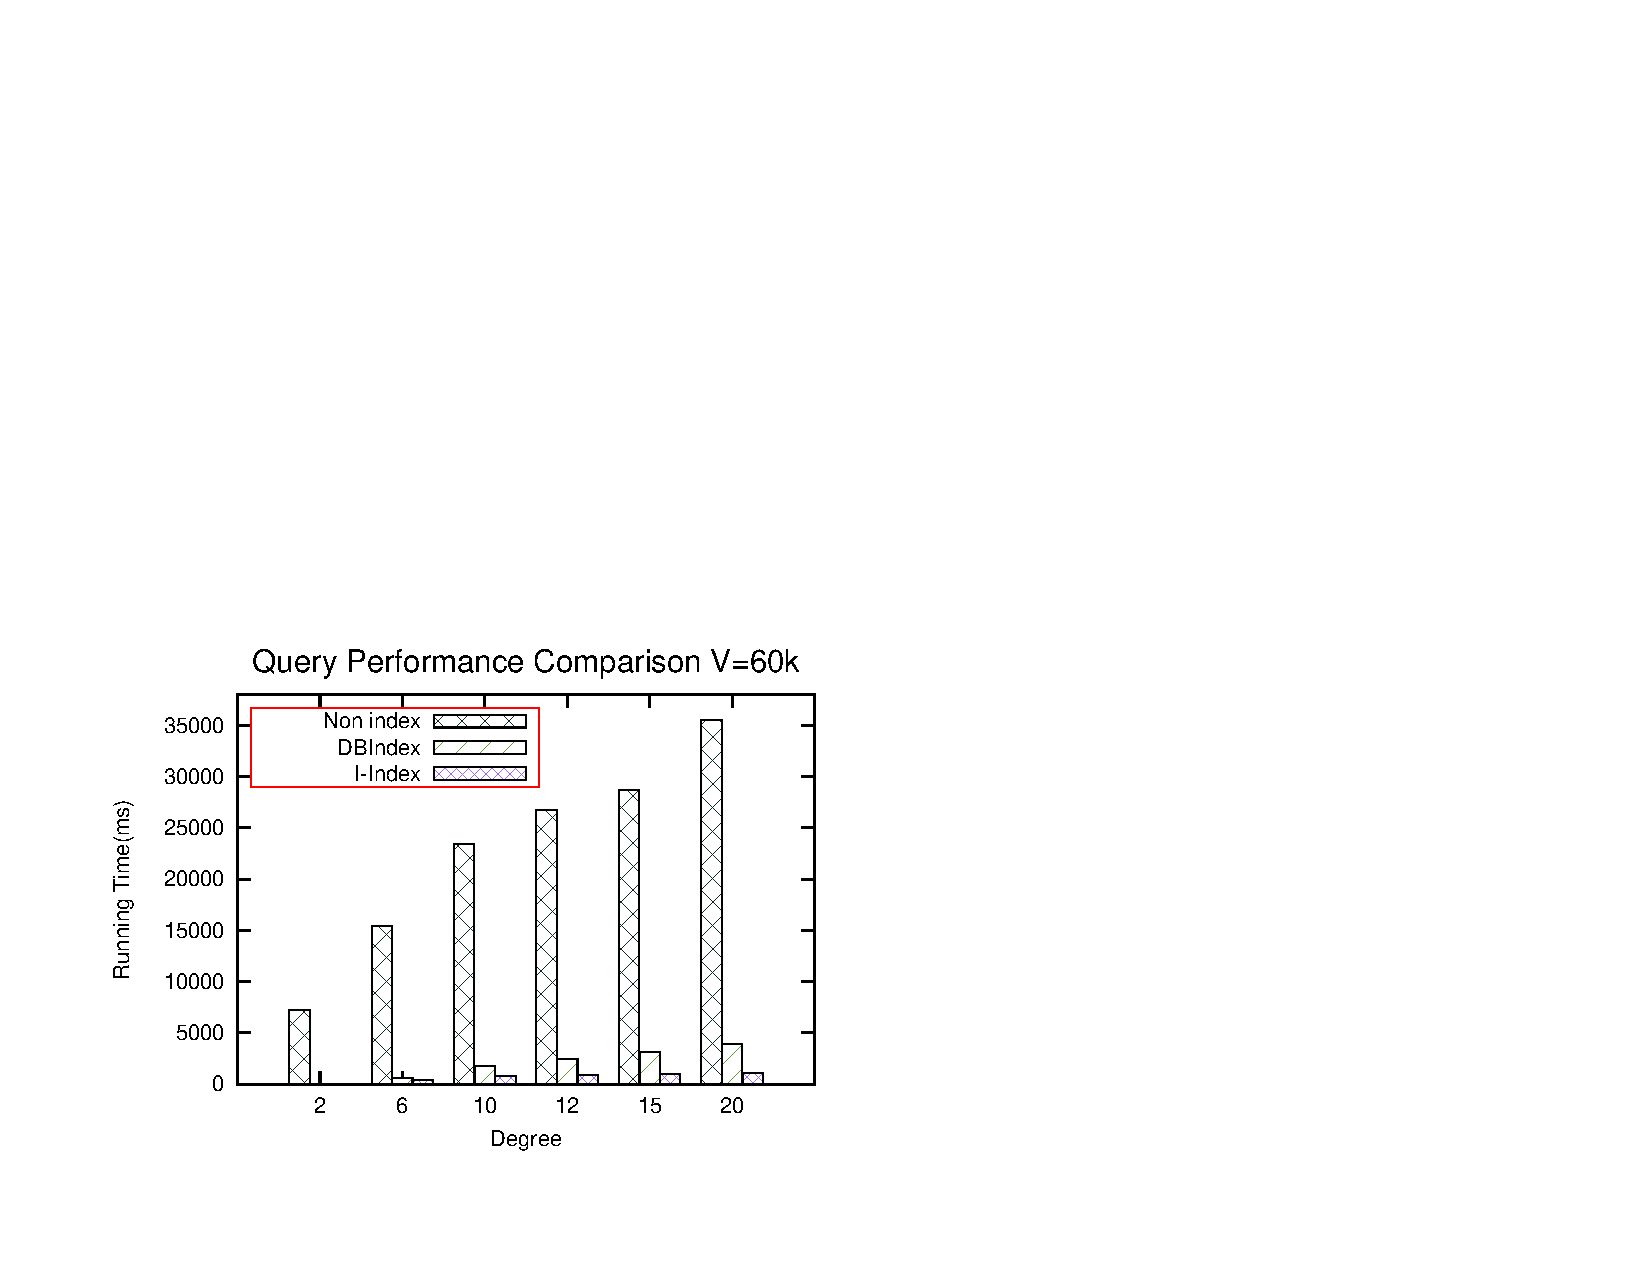
\includegraphics[width=\textwidth]{chapter3/exp/topoeffect/comp/top_query_time_v60k.pdf}
  \caption{Query performance}
\end{subfigure}
\caption{Impact of degree with the fixed number of vertexes.}
\label{fig:pi_effect}
\end{figure}

\textbf{Impact of Degree.} We evaluate the impact of degree when we fix the number of vertex as 30k and 60k.  
We compare \emph{DBIndex} with I-Index. 
In the query results, we also implement one non-index algorithm 
which dynamically calculates the window and then performs the aggregation. 
For index construction time, as shown in Figures~\ref{fig:pi_effect} (a) and (c), as the 
index size increases, both the index construction time of 
DBIndex and I-Index increase. However I-Index is more efficient than 
DBIndex, this is benefit from the inheritance optimization.  We observe that the 
index construction time is almost the same as the non-indexed query time. In other words, 
we can use one query time to create the index which is able to subsequently provide much faster query processing. 
In terms of query performance, shown in Figures~\ref{fig:pi_effect} (b) and (d), the non-index approach is in average 20 times slower than 
the indexed schemes. Meanwhile, I-Index outperforms DBIndex by 20\% to 30\%, which confirms the superiority of I-Index.
%The results clearly show that I-Index outperforms DBIndex for topological 
%window in both index construction and query performance.
%Since I-Index is superior, in the following experiments, we only present the results for I-Index. 

\textbf{Impact of Number of Vertexes.} Then, we study 
the effect of graph size by varying the number of vertexes from 50k to 350K.
%the performance of I-Index 
% is affected when we fix the degree and vary the number of Vertexes from 50k to 350K. 
Figures~\ref{fig:pi_effect2} (a) and (c) show the index construction time when we fix the degree to 
10 and 20 respectively. From the results, we see that the construction time increases as the number of vertexes increases and the construction time of a high degree graph is longer than that for low the degree graph. Figures~\ref{fig:pi_effect2} (b) and (d) show the query time when we fix the degree to 10 and 20 respectively. 
As shown, the degree affects the query processing time: when the degree increases, the query time increases as well. We also observe that the query time is increasing linearly when the number of vertexes increases. This shows that I-Index has good scalability.
  
\begin{figure}[t]
\centering
\begin{subfigure}{0.45\linewidth}
  \centering
  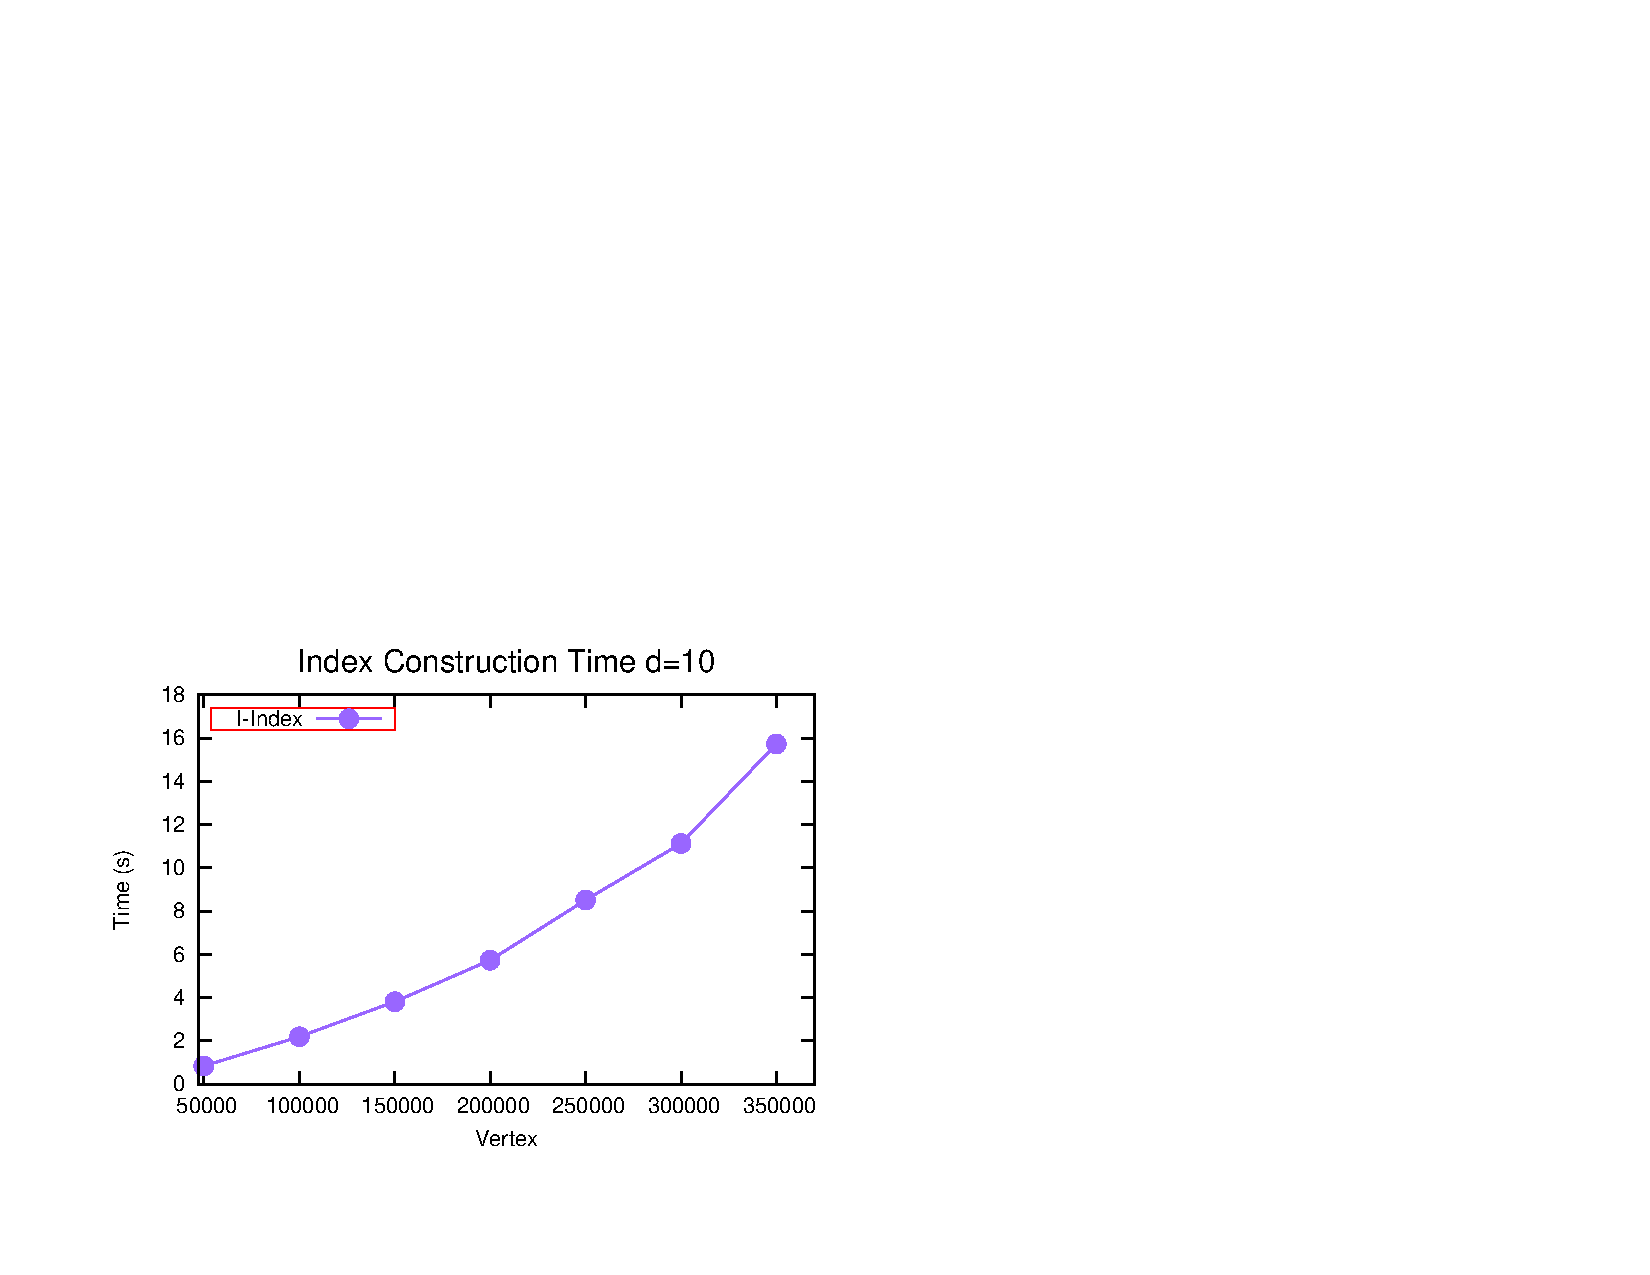
\includegraphics[width=\textwidth]{chapter3/exp/topoeffect/comp/top_scale_index_d10.pdf}
  \caption{Index construction }
\end{subfigure}
\begin{subfigure}{0.45\linewidth}
  \centering
  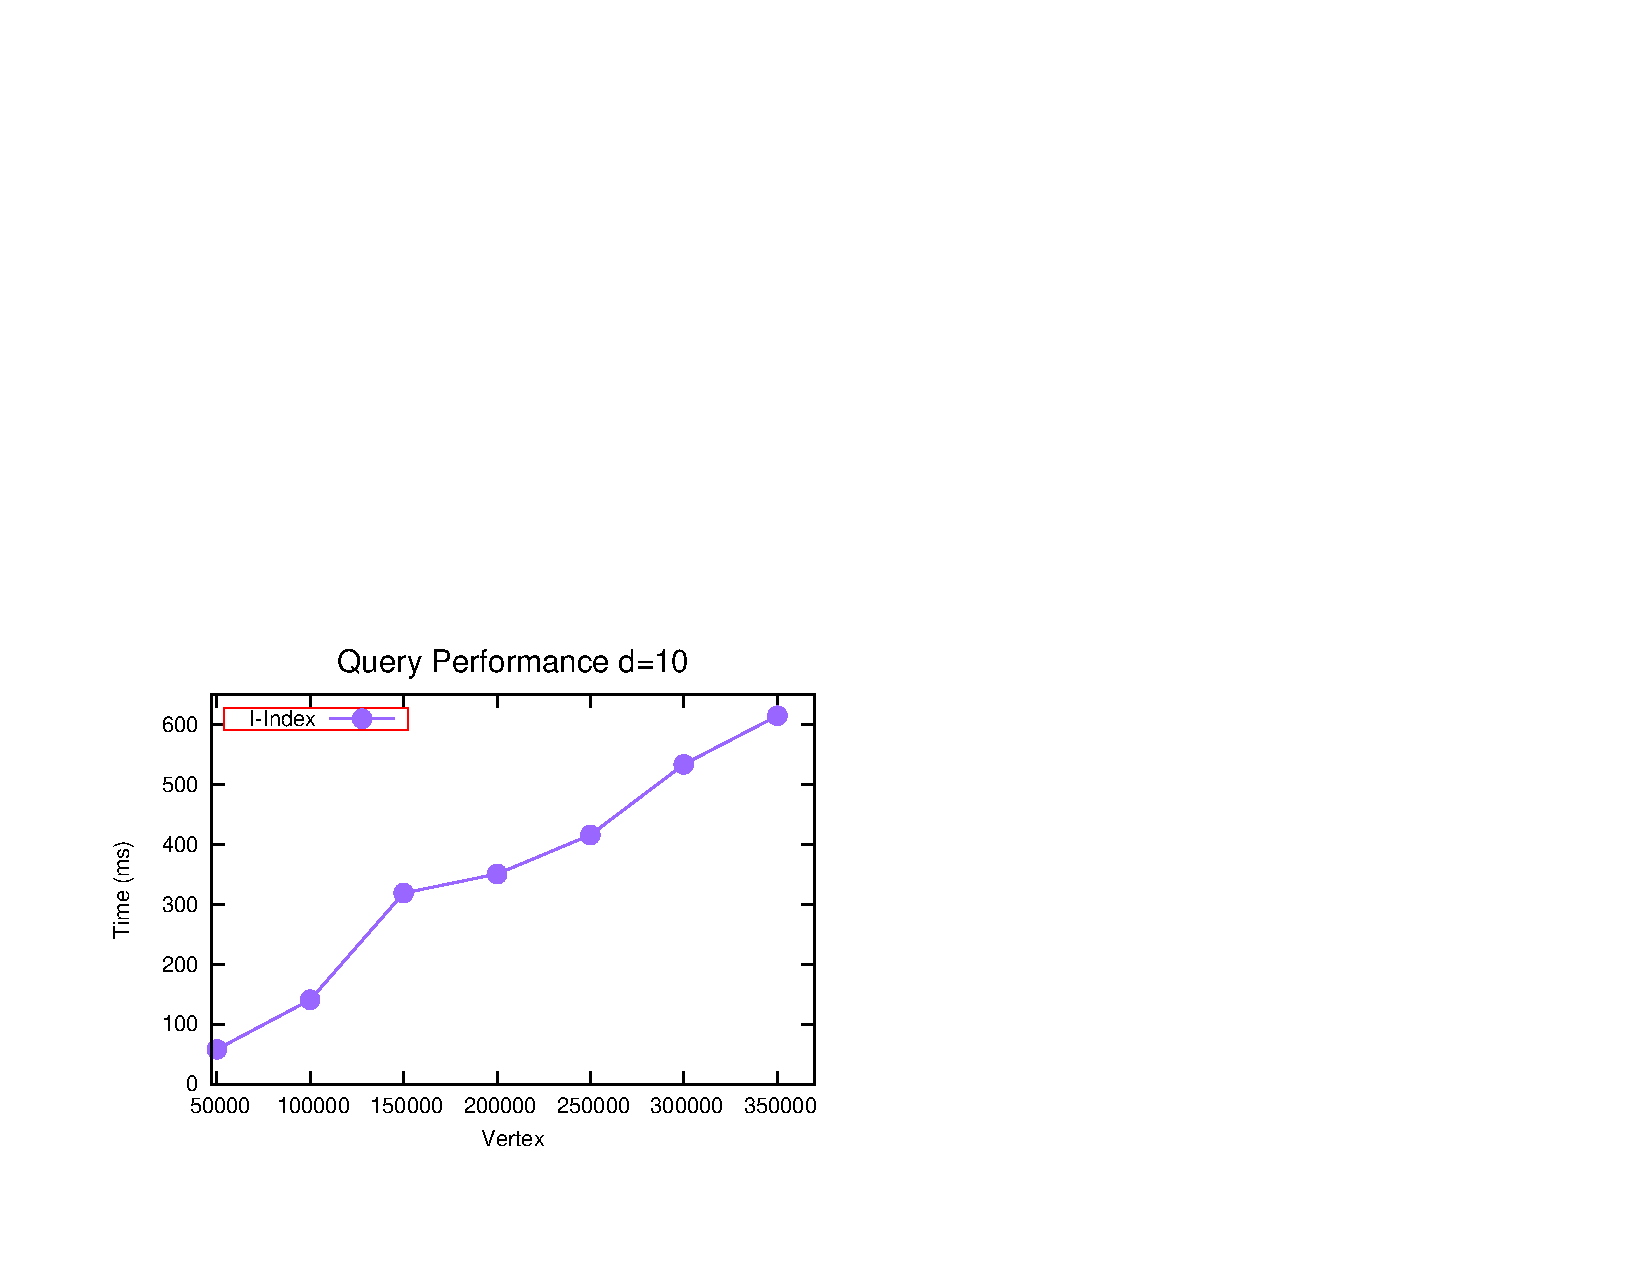
\includegraphics[width=\textwidth]{chapter3/exp/topoeffect/comp/top_scale_query_d10.pdf}
  \caption{Query performance}
\end{subfigure}
\begin{subfigure}{0.45\linewidth}
  \centering
  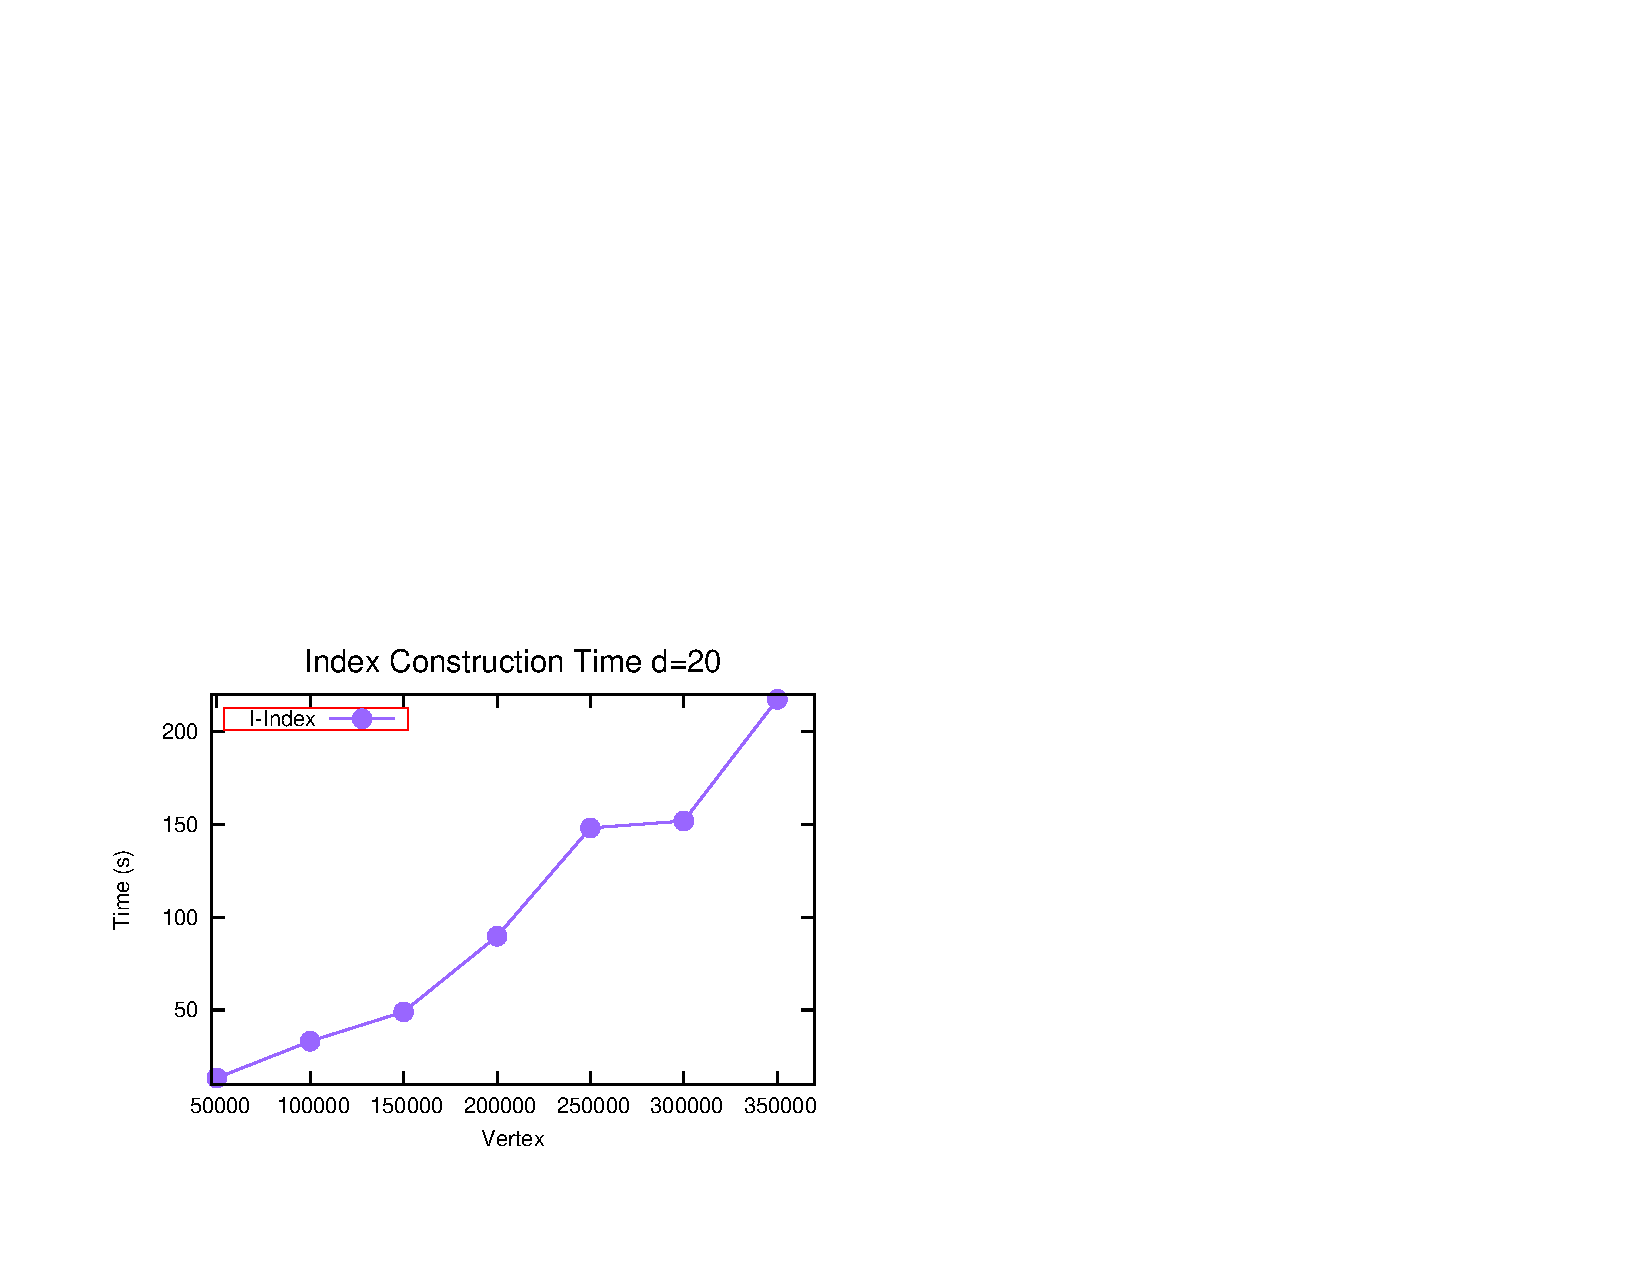
\includegraphics[width=\textwidth]{chapter3/exp/topoeffect/comp/top_scale_index_d20.pdf}
  \caption{Index construction}
\end{subfigure}
\begin{subfigure}{0.45\linewidth}
  \centering
  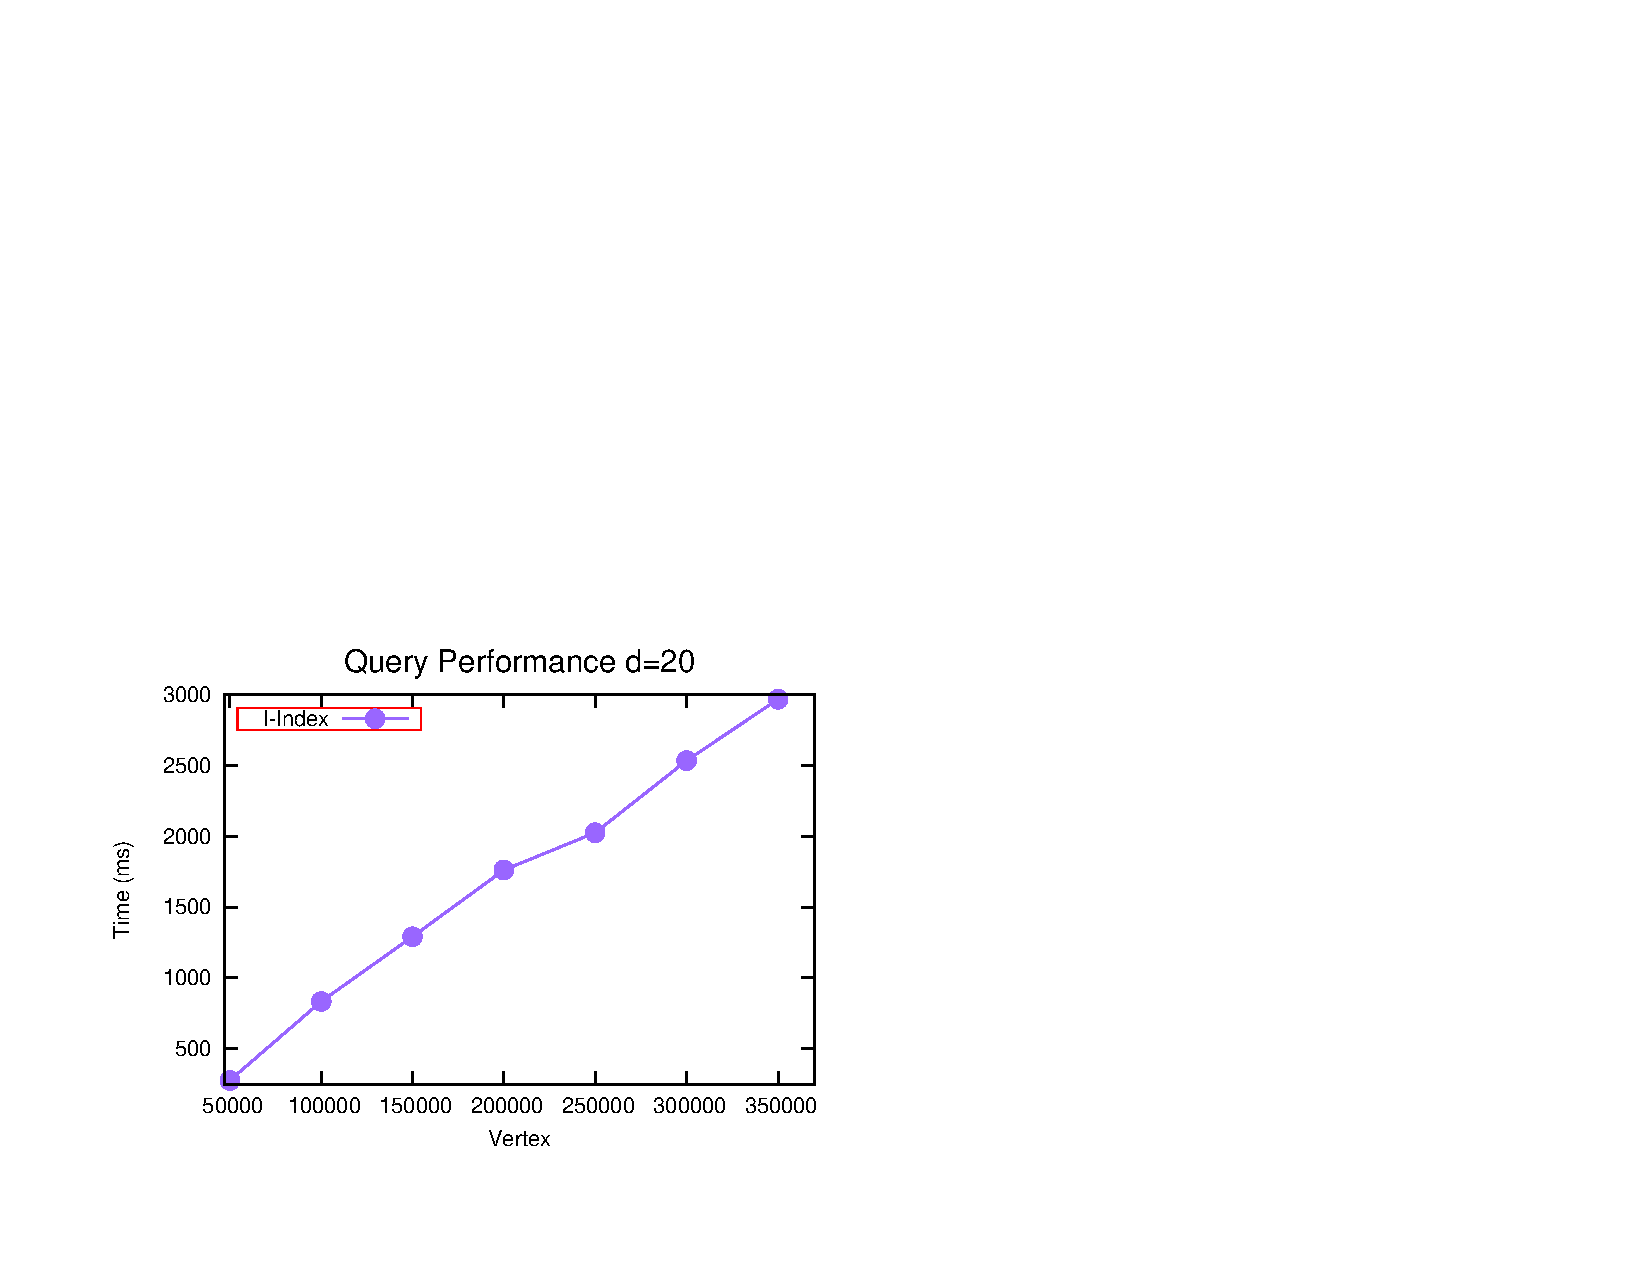
\includegraphics[width=\textwidth]{chapter3/exp/topoeffect/comp/top_scale_query_d20.pdf}
  \caption{Query performance}
\end{subfigure}
\caption{Impact of the number of vertexes with a fixed degree. (a) and (b) 
are the results for the graphs with degree 10; (c) and (d) 
are the graphs with degree 20. }
\label{fig:pi_effect2}
\end{figure}

\begin{figure}[h]
\centering
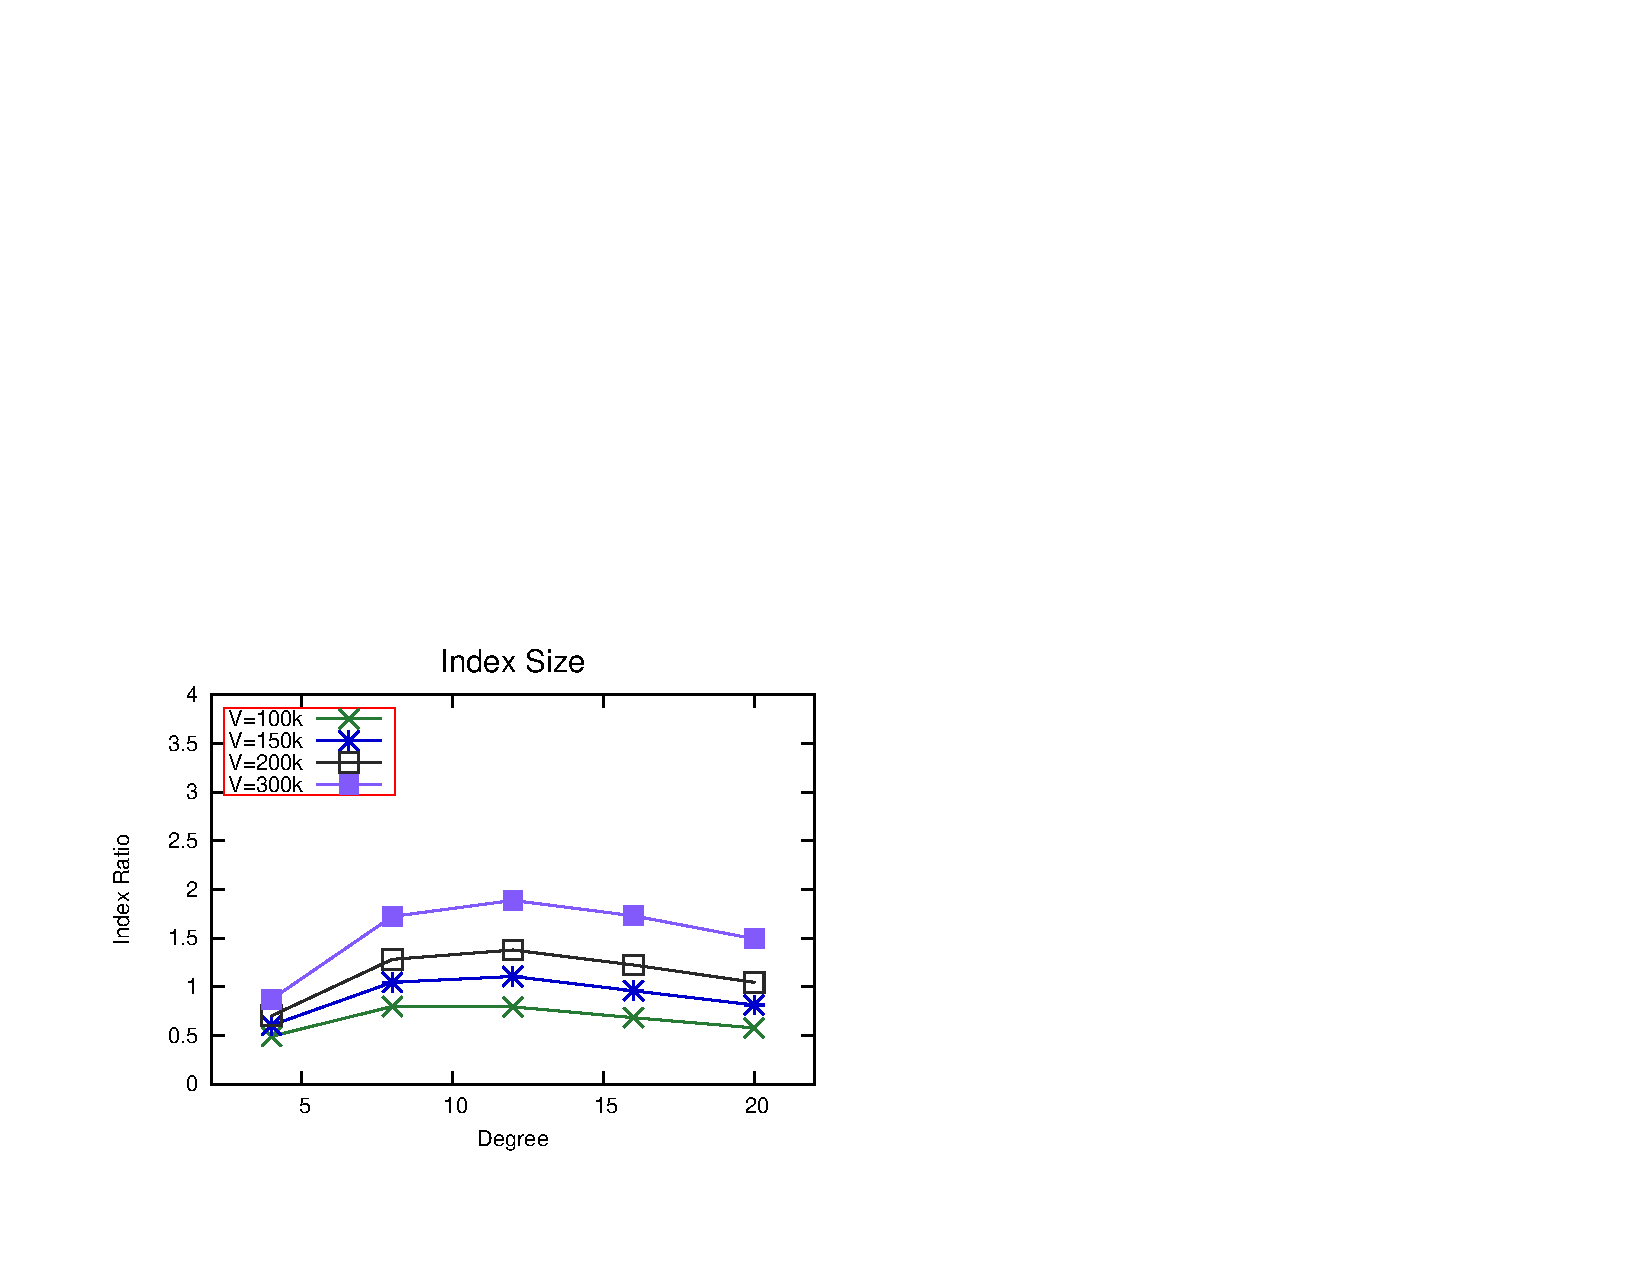
\includegraphics[width=0.5\textwidth]{chapter3/exp/topoeffect/comp/top_scale_index_size.pdf}
\caption{Index ratio of I-Index.}
\label{fig:top-index-size}
\end{figure}


\textbf{Index Size.} Figure~\ref{fig:top-index-size} presents
the index size ratio (i.e. size of index divided by the size of original graph) under different degrees from 3 to 20. 
There are four different sizes of data used with 100k, 150k, 200k and 300k vertexes.  
For every vertex setting, the index size maintains the same trend in various degrees. The index size is linear to the input graph size. 
As a graph gets denser, the difference field of the I-Index
effectively shrinks. Thus, the index size in turn becomes smaller, which explains the bends in the figure.





\section{Chapter Summary} \label{sec:conclusion}
In this chapter, we look at the problem of automatically summarize 
a subject's history using newsworthy stories.
We group consecutive events into streaks and propose a novel idea of \emph{ranked-streak} to represent the strikingness.
We then formulate the \emph{$k$-Sketch} query which aims to best summarize a subject's history using $k$ ranked-streaks.
We study the $k$-Sketch query processing in both offline and online scenarios,
and propose efficient solutions to cope each scenario. In particular, we design novel streak-level pruning techniques and a $(1-1/e)$-approximate algorithm to achieve efficient processing in offline. Then we design a $1/8$-approximate algorithm for the online sketch maintenance.
Our comprehensive experiments demonstrate the efficiency of our solutions and a human study confirms the effectiveness of the $k$-Sketch query.

%Our work opens a wide area of research in computational journalism. 
%In our next step, we aim to extend the event sources from sensor data 
%to non-schema data such as tweets in social networks. We also aim to 
%investigate subject association models to automatically generate 
%news themes involving multiple subjects.
%We further wish to explore leveraging big data technology to support fast-growing 
%event data in journalism. 
\chapter{Efficient $k$-Sketch Discovery in Sequence Data}

\chapter{A General Framework for Mining General Co-movement Patterns over Large-scale Trajectory Databases}

\section{Introduction}
Information networks such as social networks, 
biological networks and phone-call networks are 
typically modeled as graphs \cite{chen2008graph}
where the vertexes correspond to objects and the edges
capture the relationships between these objects.
For instance, in social networks, every user is represented by
a vertex and the friendship between two users is reflected by an edge between
the vertexes. In addition, a user's profile can be maintained as
the vertex's attributes. Such graphs contain a wealth of valuable 
information which can be analyzed to discover interesting patterns. 
For example, we can find the top-k influential users who can 
reach the most number of friends within 2 hops. With increasingly
larger network sizes, it is becoming significantly challenging to 
query, analyze and process these graph data. Therefore, there is an urgent need 
to develop effective and efficient mechanisms over graph data to draw out
information from such data resources.
 
Traditionally, in relational DBMS, window functions have been commonly
used for data analytics \cite{cao2012optimization, bellamkonda2013adaptive}. 
Instead of performing analysis (e.g., ranking, aggregate) over the entire data set, 
a window function returns for each input tuple a value derived from applying the function over a window of 
neighboring tuples. For instance, users may be interested in finding 
each employee's salary ranking within the department. Here,
each tuple's neighbors are essentially records from the same department.

%Interestingly, we find that the locality feature in graph scenario has even more importance than in relational data. In graph data, the graph structure indicates the relationship among different objects. In graph analysis, it is often useful to quantify a structural range to each vertex and perform analytic over the range. For instance, in a social network, it is important to detect one person's social position and influence in his/her social community. In this paper, we are motivated to extend the window queries in traditional SQL into the graph analysis. However, the window definition in the SQL is no longer applicable in graph context, as it does not capture the graph structure information which has a strong meaning in the graph data. 

Interestingly, the notion of window functions turns out to be not uncommon
in graph data. For instance, in a social network, it is important to detect 
a person's social position and influence among his/her social community. 
The ``social community'' of the person is essentially his/her ``window'' 
comprising neighbors derived from his/her k-hop friends.
However, as illustrated in this example, the structure of a graph
plays a critical role in determining the neighboring data of a vertex.
In fact, it is often useful to quantify a structural range to each vertex 
and then perform analytics over the range. 
Surprisingly, though such a concept of window functions has been widely
used, the notion has not been explicitly formulated. 
In this paper, we are motivated to extend the window queries in traditional 
SQL for supporting graph analysis. However, the window definition in 
SQL is no longer applicable in a graph context, as it does not capture 
the graph structure information.
% which has a strong meaning in the graph data. 
Thus, we seek to formulate the notion of graph windows and to develop
efficient algorithms to process them over large scaled graph structures. 

We have identified two instances of graph windows, namely 
$k${\em -hop} and {\em topological} windows. 
We first demonstrate these window semantics with the following examples. 
\begin{example}
\label{query:linkedin-2-hop-window}
\emph{(k-hop window)} In a social network ( such as Linked-In and Facebook etc.), users are normally modeled as vertexes and connectivity relationships are modeled as edges. In social network scenario, it is of great interest to summarize the most relevant connections to each user such as the neighbors within 2-hops. Some analytic queries such as summarizing the related connections' distribution among different companies, and computing age distribution of the related friends can be useful. In order to answer these queries, collecting data from every user's neighborhoods within 2-hop is necessary.
\end{example}

\begin{example}
\label{query:bio-dag-window}
\emph{(Topological window)} In biological networks (such as Argocyc, Ecocyc etc.\cite{keseler2005ecocyc}), genes, enzymes and proteins are vertexes and their dependency in a pathway are edges. Because these networks are directed 
and acyclic, in order to study the protein regulating process, one may be 
interested to find out the statistics of molecules in each protein 
production pathway. For each protein, we can traverse the graph to find 
every other molecule that is in the upstream of its pathway. Then we can group and count the number of genes and enzymes among those molecules. 
\end{example}

A common feature among these examples is that data aggregation is needed based on a set of vertexes (which is the {\em graph window}) 
defined according to each vertex.  To illustrate, in Example~\ref{query:linkedin-2-hop-window}, every user needs to gather data from its friends and friends-of-friends. 
The \emph{2-hop neighbors} form its window. Likewise, in Example~\ref{query:bio-dag-window}, every protein needs to count the number of particular type of genes preceding it in the regulating pathway. For every protein, the set of
\emph{preceding molecules} forms its window. 

To support the analyses in the above-mentioned examples, we propose a new 
type of query, \emph{Graph Window Query} (GWQ in short),
over a data graph. \emph{GWQ} is defined with respect to a graph structure 
and is important in a graph context. Unlike the traditional window in SQL, 
we identify two types of useful graph windows according to the 
graph structures, namely k-hop Window $W_{kh}$ and Topological Window $W_t$. 
A k-hop window forms a window for one vertex by using its k-hop neighbors. 
k-hop neighbors are important to one vertex, as these are the vertexes 
showing structural closeness as in Example~\ref{query:linkedin-2-hop-window}. The k-hop neighbors window 
we define here is similar to the egocentric-network in network analysis \cite{burt2009structural} \cite{mondal2014eagr}. A topological window, on the
other hand, forms a window for one vertex by using all its preceding 
vertexes in a directed acyclic graph. The preceding vertexes of one vertex are normally those which influence the vertex in a network as illustrated in Example~\ref{query:bio-dag-window}. 

To the best of our knowledge, existing graph databases or graph query languages do not directly support our proposed GWQ. There are two major challenges in processing GWQ. First, we need an efficient scheme to  calculate the window of each vertex. Second, we need
efficient solutions to process the aggregation over a large number 
of windows that may overlap. This offers opportunities to share the 
computation. However, it is non-trivial to address these two challenges.  

For $k$-hop window like query, the state-of-the-art processing algorithm
is EAGR \cite{mondal2014eagr}. EAGR builds an overlay graph including 
the shared components of different windows. This is done 
in multiple iterations, each of which performs the following.
First, EAGR sorts all the vertexes according to their $k$-hop 
neighbors based on their lexicographic order. 
Second, the sorted vertexes are split into equal sized chunks each of which is further built as one frequent-pattern tree to mine the shared components. 
However, EAGR requires all the vertexes' $k$-hop 
neighbors to be pre-computed and resided in memory during 
each sorting and mining operation;
otherwise, EAGR incurs high computation overhead if the pre-computed structure needs to be shuffled to/from disk.
This limits the efficiency and scalability of EAGR.
 For instance, 
a LiveJournal social network graph\footnote{Available at http://snap.stanford.edu/data/index.html, which is used in \cite{mondal2014eagr}} 
(4.8M vertices, 69M edges) generates over 100GB neighborhood information 
for k=2 in adjacency list representation. In addition, the overlay graph construction is not a one-time task,
but periodically performed after a certain number of structural updates in order to maintain the overlay quality. The high memory consumption renders the scheme impractical 
when $k$ and the graph size increases.

In this paper,
we propose \textit{Dense Block Index (DBIndex)} 
to process queries efficiently.
Like EAGR, DBIndex seeks to exploit common
components among different windows to salvage 
partial work done. However, unlike EAGR,
we identify the window similarity utilizing a hash-based 
clustering technique instead of sorting. This ensures 
efficient memory usage, as the window information of each vertex can 
be computed on-the-fly. On the basis of the clusters, we develop different optimizations 
to extract the shared components which result in an efficient index construction. 

Moreover, we provide another \emph{Inheritance Index (I-Index)} tailored 
to topological window query. I-Index differentiates itself from
DBIndex by integrating more descendant-ancestor relationships 
to reduce repetitive computations. This results in
%to reduce the repetitive computation. This results in
more efficient index construction and query processing.  

 
Our contributions are summarized as follows:
\begin{itemize}
\item{We propose a new type of graph analytic query, \emph{Graph Window Query} and formally define two graph windows: k-hop window and topological window. We illustrate how these window queries would help users better query and
understand the graphs under these different semantics.}

\item{ To support efficient query processing, we further propose two different types of indexes: \emph{Dense Block Index} (DBIndex) and \emph{Inheritance Index} (I-Index). The
\emph{DBIndex} and \emph{I-Index} are specially 
optimized to support k-hop window and topological window query processing. 
We develop the indices by integrating the window aggregation sharing techniques to salvage partial work done for efficient computation. In addition, we develop space and performance efficient techniques for index construction. 
Compared to EAGR \cite{mondal2014eagr}, the state-of-the-art index method for k-hop window queries, our DBIndex is much more memory efficient and scalable towards handling the large-scale graphs. }

\item{We perform extensive experiments over both real and synthetic datasets
with hundreds of millions of vertexes and edges on a single machine. Our experiments 
indicate that our proposed index-based algorithms outperform the naive non-index
algorithm 
by up to four orders of magnitude. In addition, our experiments also show 
that DBIndex is superior over EAGR in terms of both
scalability and efficiency. In particular, 
DBIndx saves up to 80\% of indexing time as 
compared to EAGR, 
and performs well even when EAGR fails due
to memory limitations. 
}
\end{itemize}

\section{Related Work}\label{sec:related_work}
In this section, we briefly review three closely related areas: automatic news theme detection, frequent episode mining and top-$k$ diversity query.

\subsection{Automatic News Theme Detection}
Earlier works on automatic news theme generation were focused on finding interesting themes from a single event. For example, Sultana et al.~\cite{sultana2014incremental} proposed the \emph{Situational Fact} pattern, which is modeled as a skyline point under certain dimensions. Wu et al.~\cite{wu2012one} proposed the \emph{One-of-the-Few} concept to detect news themes with some rarities. Examples of candidate news themes for the above two patterns are illustrated in Table~\ref{tbl:related_works}.

{\renewcommand{\arraystretch}{1.2} 
\begin{table}[h]
\centering
\begin{tabular}{|l|l|}
\hline
\textbf{Method} & \textbf{Example news theme}\\
\hline
Situational facts~\cite{sultana2014incremental} & \pbox{22cm}{\vspace{.3\baselineskip} Ellen's tweet generates 3.3M retweets\\ with 170,000 comments.\vspace{.3\baselineskip}} \\
\hline
One-of-the-few facts~\cite{wu2012one} & \pbox{22cm}{\vspace{.3\baselineskip}Perry is one of the three candidates \\  who received \$600k. \vspace{.3\baselineskip}} \\
\hline
Prominent streak~\cite{zhang2014discovering} & Kobe scored 40+ in 9 straight games!  \\
\hline
Rank-aware theme & \pbox{22cm}{\vspace{.3\baselineskip}Kobe scored 40+ in 9 straight games\\ ranked 4th in NBA history!\vspace{.3\baselineskip}} \\
\hline
\end{tabular}
\label{tbl:related_works}
\caption{Examples of different news themes}
\end{table}
}

Zhang et al.\cite{zhang2014discovering} proposed using prominent streaks to generate interesting news themes.
In \cite{zhang2014discovering}, a \emph{Prominent Streak} is characterized by a 2D point which represents the window length and the minimum value of all events in the window. The objective is to discover the non-dominated event windows for each subject, where the dominance relationship is defined among streaks of the same subject. Our model differs from \cite{zhang2014discovering} in two aspects. First, we look at the global prominence (quantified by the rank) among all subjects rather than local prominence (quantified by the dominance) within one subject. Second, our model provides the best $k$-sketch for each subject whereas \cite{zhang2014discovering} returns a dominating set which could be potentially large. 
 
\subsection{Frequent Episode Mining}
In time sequenced data mining, an episode~\cite{mannila1997discepisodes,
zhou2010serialepisodes, tatti2012strictepisodes, laxman2007nonoverlapepisodes} is 
defined as a collection of time sequenced events which occur together within a time window. The uniqueness of an episode is determined by the contained events. The objective is to discover episodes whose 
occurrences exceeding a support threshold. 
Our sketch discovery differs from the episode mining in three major aspects. First, an episode is associated with a categorical value while our sketch is defined on numerical values. Second, the episodes are selected based on the occurrence, while in sketch, news themes are generated in a rank-aware manner. Finally, episode mining does not restrict its output size, while sketch only outputs the best $k$ news themes. As such, episode mining techniques cannot be straightforwardly applied to sketch discovery.

%First, episode concerns event types (alphabets), while streak concerns the analytic values. The mismatch makes episode mining inappropriate for sketch discovery since counting the occurrence based on analytic values is not meaningful. Second, candidate episode is selected based on the number of occurrence compared to a threshold, whereas candidate streak is based on the rank among other streaks with the same window size. The notion of rank does not straightforwardly apply to episodes thus making the problem different from sketch discovery. Third, in sketch discovery, we aim to find the best $k$ streaks, while in episode mining, there is no evaluation among episodes thus it does not fit the needs of sketch discovery.


\subsection{Top-$k$ Diversity Query}
Top-$k$ diversity queries~\cite{agrawal2009diversifying,borodin2012max,drosou2014diverse,chen2015diversity}
aim to find a subset of objects to maximize a scoring function. The scoring function normally penalizes
a subset if it contains similar elements. Our sketch discovery problem has two important distinctions
 against the top-$k$ diversity queries.
First, the inputs of the scoring function are known in advance in top-$k$ diversity queries; whereas in our problem, the ranks of event windows are unknown. Since their calculations are expensive, we need to devise efficient methods to compute the ranks.
Second, existing methods for online diversity queries~\cite{borodin2012max,drosou2014diverse,chen2015diversity} only study
the updates on a single result set when a new event arrives. However our online sketch maintenance 
incurs the problem of multiple sketch updates for each new event. Such a complex update pattern has not been studied yet and hence there is a need to develop efficient update scheme.

\subsection{Event Detection and Tracking}
In the information retrieval field, event detection and tracking aim to extract and organize new events from various
media sources. Allen et.al~\cite{allan1998line} first proposed the problem of detecting unseen events from text streams, where they adapted an online clustering algorithm to tackle the problem. Subsequent researches extended the problem to facilitate heterogeneous sources. For example, Brants et.al.~\cite{brants2003asystem} proposed a TF-IDF model to detect unseen events from multiple text streams. Ritter et.al.~\cite{ritter2012opendoamin} proposed a system named TwiCal to categorize events on Twitter streams. Li et.al.~\cite{li2015social} proposed a ranking model to detect events on Flickr and Vuurens et.al.~\cite{Vuurens2015Onlinenews} described a system on tracking events from web articles.

Despite the usefulness of those works, they differ from the rank-aware news themes proposed in this paper.
The major difference is that news detection and tracking focuses on detecting a single event from various sources; While
the rank-aware news theme aims at providing insightful derived events from a single source. This crucial 
difference prevents the above-mentioned techniques directly applying to our problem.


\section{Problem Formulation}
\label{sec:definition}
Let $\mathbb{O} = \{o_1 ,o_2,...,o_n\}$ be the set of objects and $\mathbb{T} =(1,2,...,N)$ be the discretized temporal dimension. A time sequence $T$ is defined as an ordered subset of $\mathbb{T}$. Given two time sequences $T_1$ and $T_2$, we define the commonly-used operators in this chapter in Table~\ref{tbl:operators}.

\begin{table}[h]
\centering
\caption{Operators on time sequence.}
\label{tbl:operators}
\begin{tabular}{|l|l|}
\hline 
\textbf{Operator} & \textbf{Definition} \\ 
\hline
$T[i]$ & the $i$-th element in the sequence $T$ \\ 
\hline
$|T|$ & the number of elements in $T$\\
\hline
$\max(T)$ & the maximum element in $T$\\
\hline
$\min(T)$ & the minimum element in $T$\\
\hline
$\range(T)$ & the range of $T$, i.e., $\max(T) - \min(T) +1$\\ 
\hline 
$T[i:j]$ & subsequence of $T$ from $T[i]$ to $T[j]$ (inclusive) \\ 
\hline
$T_1\subseteq T_2$ &  $\forall T_1[x]\in T_1$, we have $T_1[x]\in T_2$. \\\hline
$T_3=T_1\cup T_2$ & $\forall T_3[x]\in T_3$, we have $T_3[x]\in T_1$ or $T_3[x] \in T_2$\\ 
\hline
$T_3=T_1\cap T_2$ & $\forall T_3[x]\in T_3$, we have $T_3[x]\in T_1$ and $T_3[x] \in T_2$\\ 
\hline
\end{tabular}
\end{table} 

We say a sequence $T$ is consecutive 
if $\forall 1 \leq i < |T|, T[i+1] = T[i] + 1$.  We refer to each consecutive subsequence of $T$ as a \emph{segment}.
It is obvious that any time sequence $T$ can be decomposed into one or more
segments and we say $T$ is \textit{L-consecutive}~\cite{li2015platoon} 
if the length of every segment is no smaller than $L$. As illustrated in Figure~\ref{fig:platoon_weakpoint}, patterns adopting the notion of $L$-consecutiveness (e.g., \emph{platoon} and \emph{group}) still suffer from the \emph{loose-connection} anomaly. 
To avoid such an anomaly without losing generality, we introduce a parameter $G$ to control the gaps between
timestamps in a pattern. Formally, a $G$-connected time sequence is defined as follows:

\begin{definition}[$G$-connected]
A time sequence $T$ is $G$-connected if the gap between any of its neighboring timestamps is no greater than $G$, i.e., $\forall 1 \leq i < |T|, T[i+1]-T[i] \leq G$.
\end{definition}

We take $T=(1,2,3,5,6)$ as an example. $T$ can be decomposed into two segments $(1,2,3)$ and $(5,6)$. $T$ is not $3$-consecutive since the length of $(5,6)$ is $2$. But it is safe to say either $T$ is $1$-consecutive or $2$-consecutive. On the other hand, $T$ is $2$-connected since the maximum gap between its neighboring timestamps is $2$. It is worth noting that $T$ is not $1$-connected because the gap between $T[3]$ and $T[4]$ is $2$ (i.e., $5-3=2$).

Given a trajectory database that is discretized into snapshots, we can conduct a clustering method, either disk-based or density-based, to identify groups with spatial proximity. Let $T$ be the set of timestamps in which a group of objects $O$ are clustered. We are ready to define a more general co-movement pattern:
\begin{definition}[General Co-Movement Pattern]
A general co-movement pattern finds a set of objects $O$ satisfying the following five constraints: (1) \textbf{closeness:} the objects in $O$ belong to the same cluster in every timestamps of $T$; (2) \textbf{significance:} $|O| \geq M$; (3) \textbf{duration:} $|T| \geq K$; (4) \textbf{consecutiveness:} $T$ is $L$-consecutive; and (5) \textbf{connection:} $T$ is $G$-connected.
\end{definition}
There are four parameters in our general co-movement pattern, including object constraint $M$ and temporal constraints $K,L,G$. 
%\revised{These parameters have different effects on the number of patterns discovered. Larger $K$, $L$, $M$ 
%put more stringent constraints on patterns such that less patterns could satisfy the requirements. Larger $G$
%relaxes the temporal constraints therefore more patterns could be discovered. Currently, we leave tuning of
%parameters to users to accommodate various application needs.}  
By customizing these parameters, our pattern can 
express other patterns proposed in the literature, as illustrated in Table~\ref{tbl:patterns}. 
In particular, by setting $G=|\mathbb{T}|$, we achieve the \emph{platoon} pattern. By setting $G=|\mathbb{T}|,L=1$, we reach the \emph{swarm} pattern. By setting $G=|\mathbb{T}|$, $M=2$, $K=1$, we gain the \emph{group} pattern. Finally by setting $G=1$, we result in the \emph{convoy} and \emph{flock} patterns. 
In addition to the flexibility of representing other existing patterns, our GCMP is able to avoid the \emph{loose-connection} anomaly by tuning the parameter $G$. 
%It is notable that GCMP cannot be modeled by existing patterns. 
\begin{table}[h]
\centering
\caption{Expressing other patterns using GCMP. $\cdot$ indicates a user specified value.}
\label{tbl:patterns}
\begin{tabular}{|l|c|c|c|c|c|}
\hline 
\textbf{Pattern} & $M$ & $K$ & $L$ & $G$ & \textbf{Clustering} \\ 
\hline
Group & $2$ & $1$ & $2$ & $|\mathbb{T}|$ & disk\\
\hline
Flock & $\cdot$ & $\cdot$ & $K$ & $1$ & disk \\
\hline 
Convoy & $\cdot$ & $\cdot$ & $K$ & $1$ & density\\ 
\hline 
Swarm & $\cdot$ & $\cdot$ & $1$ & $|\mathbb{T}|$ & density\\ 
\hline 
Platoon & $\cdot$ & $\cdot$ & $\cdot$ & $|\mathbb{T}|$ & density\\  
\hline 
\end{tabular} 
\end{table}

Our definition of GCMP is independent of the clustering method. Users can apply different clustering methods to facilitate different application needs. 
We currently expose both disk-region based clustering and DBSCAN as options to the users. In summary, the goal of this work is to present a parallel solution for discovering all the valid GCMPs from large-scale trajectory databases. Before we move on to the algorithmic part, we list the notations that are used in the following sections.

\begin{table}[h]
\centering
\caption{Summary of notations.}
\begin{tabular}{|c|l|} 
\hline
\textbf{Symbol} & \textbf{Meaning} \\
\hline
$S_t$ & snapshot of objects at time $t$ \\
\hline
$M$ & significance constraint \\
\hline 
$K$ & duration constraint\\
\hline
$L$ & consecutiveness constraint\\
\hline
$G$ & connection constraint \\
\hline
$P=\langle O:T \rangle$ & pattern with object set $O$, time sequence $T$\\
\hline
%$C_t(o)$ & cluster of object $o$ at time $t$ \\
%\hline 
$S_t$ & set of clusters at snapshot $t$\\
\hline
$\eta$ & replication factor in the TRPM framework\\
\hline 
$\lambda_t$ & partition with snapshots $S_t,..,S_{t+\eta-1}$ \\
\hline
$G_A$ & aggregated graph in SPARE framework\\
\hline
$Sr_i $ &  star partition for object (vertex) $i$ \\
\hline 
%$\Gamma$ & size of the largest star partition\\
%\hline
\end{tabular} 
\end{table}
\begin{figure*} [t]
\center
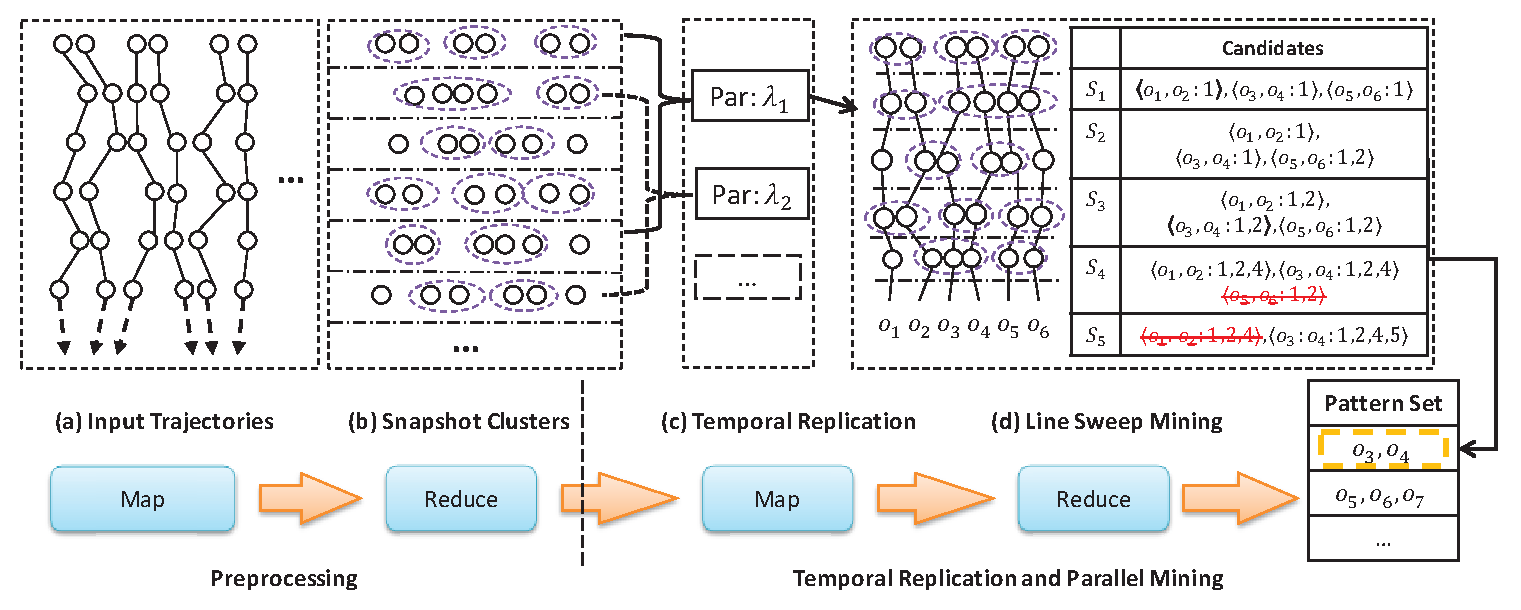
\includegraphics[width=\textwidth]{chapter5/trm.eps}
\caption{Work flow of Temporal Replication and Parallel Mining (TRPM). (a) and (b) correspond to the first map-reduce stage which clusters objects in each snapshot.  (c) and (d) correspond to the second map-reduce stage, which uses TRPM to detect GCMP in parallel.}
\label{fig:trm}
\end{figure*}

\section{Baseline: Temporal Replication and Parallel Mining}
\label{sec:trm}
In this section, we propose a baseline solution that resorts to MapReduce (MR) as a general, parallel and scalable paradigm for GCMP mining. The framework, named \textit{temporal replication and parallel mining} (TRPM), is illustrated in   Figure~\ref{fig:trm}. There are two stages of map-reduce jobs connected in a pipeline manner. The first stage deals with spatial clustering of objects in each snapshot, which can be seen as a preprocessing step for the subsequent pattern mining phase. In particular, for the first stage, the timestamp is treated as the key in the map phase and objects within the same snapshot are clustered (DBSCAN or disk-based clustering) in the reduce phase. Finally, the reducers output clusters of objects in each snapshot, represented by a list of key-value pairs $\langle t, S_t  \rangle$, where $t$ is the timestamp and $S_t$ is a set of clustered objects at snapshot $t$. 

Our focus in this paper is on the second map-reduce stage of parallel mining, which essentially addresses two key challenges. The first is to ensure effective data partitioning such that the mining on each partition can be conducted independently; and the second is to efficiently mine the valid patterns within each partition. 

It is obvious that we cannot simply split the trajectory database 
into disjoint partitions because a GCMP requires $L$-consecutiveness 
and the corresponding segments may span multiple partitions. 
Our strategy is to use data replication to enable parallel mining. 
Each snapshot will replicate its clusters to $\eta-1$ preceding snapshots.
In other words, the partition for the snapshot $S_t$ contains clusters 
in $S_t$, $S_{t+1}\ldots,S_{t+\eta-1}$. 
Determining a proper $\eta$ is critical in ensuring the
correctness and efficiency of TRPM. If $\eta$ is too small, 
certain cross-partition patterns may be missed. 
If $\eta$ is too large, expensive network communication and 
CPU processing costs would be incurred in the map and reduce phases respectively. Our objective is to find an $\eta$ that is not large but can guarantee correctness.

In our implementation, we set $\eta = (\lceil \frac{K}{L} \rceil - 1)*(G-1)+K+L-1$. Intuitively, with $K$ timestamps, at most $\lceil \frac{K}{L} \rceil - 1$ gaps may be generated as the length of each $L$-consecutive segment is at least $L$. Since the gap size is at most $G-1$, $(\lceil \frac{K}{L} \rceil - 1)*(G-1)$ is the upper bound of timestamps allocated to gaps. The remaining part of the expression, $K+L-1$, is used to capture the upper bound allocated for the $L$-consecutive segments. We formally prove that $\eta$ can guarantee correctness.


\begin{theorem}
\label{THM:RP_ETA}
$\eta = (\lceil \frac{K}{L} \rceil - 1)*(G-1)+K+L-1$ guarantees that no valid pattern is missing.
\end{theorem}
\begin{proof}
Given a valid pattern $P$, we can always find at least one valid subsequence of $P.T$ that is also valid. Let $T'$ denote the valid subsequence of $P.T$ with the minimum length. In the worst case, $T'=P.T$. We define $\range(T)=\max(T) - \min(T) +1$ and prove the theorem by showing that $\range(T') \leq \eta$.
Since $T'$ can be written as a sequence of L-consecutive segments interleaved by gaps: $l_1,g_1,\ldots,l_{n-1}$, $g_{n-1},l_n$ ($n \geq 1$),
where $l_i$ is a segment and $g_i$ is a gap. Then, $\range(T')$
is calculated as $\Sigma_{i=1}^{i=n}|l_i| + \Sigma_{i=1}^{i=n-1} |g_i|$. Since $T'$
is valid, then $\Sigma_{i=1}^{i=n}|l_i| \geq K$. As $T'$ is minimum, if we remove the 
last $l_n$, the resulting sequence should not be valid. Let $K' = \Sigma_{i=1}^{i=n-1}|l_i|$, which
is the size of the first $(n-1)$ segments of $T'$. Then, $K' \leq K-1$.
Note that every $|l_i| \geq L$, thus $n \leq \lceil \frac{K'}{L} \rceil \leq \lceil \frac{K}{L} \rceil $. By
using the fact that every $|g_i| \leq G-1$, we achieve $\Sigma_{i=1}^{i=n-1} |g_i| \leq (n-1)(G-1)
\leq (\lceil \frac{K}{L} \rceil -1)(G-1)$. Next, we consider the difference between $K$ and $K'$, denoted by
$\Delta = K- K'$. To ensure $T'$'s validity, $l_n$ must equal to $\min(L, \Delta)$.
Then, $\Sigma_{i=1}^{i=n}|l_i| = K' + l_n = K - \Delta + \min(L, \Delta) \leq K - 1 + L$. We finish showing $\range(T') \leq \eta$.  Therefore, for any valid sequence $T$, it exists at least one valid subsequence with range no greater than $\eta$ and hence this pattern can be detected in a partition with $\eta$ snapshots.
\end{proof}


\begin{algorithm}[h]
\small
\caption{Line Sweep Mining}
\label{algo:line-sweep}
\begin{algorithmic}[1]
\Require $\lambda_t = \{S_t, ..., S_{t+\eta-1}\}$
\State{$C \gets \{\}$} \Comment{Candidate set} \label{code:ls-can-set}
\ForAll{clusters $s$ in snapshot $S_t$} 
\label{code:ls-init-start}
\If{$|s| \geq M$}
\State $C\leftarrow C\cup \{\langle s, t \rangle \}$
\EndIf
\EndFor
\label{code:ls-init-end}
\ForAll{$S_j \in \{S_{t+1},\ldots,S_{t+\eta-1}\}$} \label{code:ls-sweep-starts}
	\State $N \gets \{\}$
	\ForAll {$(c,s) \in C \times S_j$} \label{code:ls-join-start}
		\State {$c' \gets \langle c.O \cap s.O, c.T \cup \{j\} \rangle$} \label{code:ls-join}
		\If {$c'.T$ is valid} 
			\State output $c'$
		\ElsIf{$|c'.O| \geq M$}
			\State $N\leftarrow N\cup \{c'\}$ \label{code:ls-m-prun}	
		\EndIf
	\EndFor \label{code:ls-join-ends}
	\ForAll {$c \in C$}
		\If{$j-\max(c.T)\geq G$}\label{code:ls-g-prune-starts}
			\State $C\leftarrow C-\{c\}$ 
			\State output $c$, if $c$ is a valid pattern
		\EndIf  \label{code:ls-g-prune-ends}
		\If{$c$'s first segment is less than $L$}\label{code:ls-l-prune-starts}
			\State $C\leftarrow C-\{c\}$ 
		\EndIf\label{code:ls-l-prune-ends}
	\EndFor
	\State $C\leftarrow C\cup N$
\EndFor\label{code:ls-sweep-ends}
\State output valid patterns in  $C$  \label{code:ls-valid-check}
\end{algorithmic}
\end{algorithm}



Based on the above theorem, under TRPM, every consecutive $\eta$ snapshots
form a partition. In other words, each snapshot $S_t$ corresponds to a partition $\lambda_t=\{S_t,...,S_{t+\eta-1}\}$. Our next task is to design an efficient pattern mining strategy within each partition. Our solution includes a line sweep algorithm to sequentially scan the $\eta$ replicated snapshots in a partition and an effective candidate pattern enumeration mechanism.  

Details of the algorithm are presented in Algorithm~\ref{algo:line-sweep}. We keep a candidate set $C$ (Line~\ref{code:ls-can-set}) during the sweeping process. It is initialized using the clusters with size no smaller than $M$ in the first snapshot. Then, we sequentially scan each snapshot (Lines~\ref{code:ls-sweep-starts}-\ref{code:ls-sweep-ends}) and generate new candidates by extending the original ones in $C$.
In particular, we join candidates in $C$ with all the clusters in $S_j$ to form new candidates (Lines~\ref{code:ls-join-start}-\ref{code:ls-join-ends}). 

After sweeping all the snapshots, all the valid patterns are stored in $C$ (Line~\ref{code:ls-valid-check}). 
It is worth noting that $C$ continues to grow during the whole sweeping process. We can use three pruning rules to early remove false candidates from $C$. Since there is a partition $\lambda_t$ for each $S_t$, only patterns that start from timestamp $t$ need to be discovered. Therefore, those patterns that do not appear in the $S_t$ are false candidates. In particular, our
three pruning rules are as follows:
First, when sweeping snapshot $S_j$, new candidates with objects set smaller than $M$ are pruned (Line~\ref{code:ls-m-prun}). Second, after joining with all clusters in $S_j$, 
candidates in $C$ with the maximum timestamp no smaller than $j-G$ are pruned (Lines~\ref{code:ls-g-prune-starts}-\ref{code:ls-g-prune-ends}). Third, candidates in $C$ with the size of the first segment smaller than $L$
are pruned (Lines~\ref{code:ls-l-prune-starts}-\ref{code:ls-l-prune-ends}). With the three pruning rules, the size of $C$ can be significantly reduced.  

The complete picture of temporal replication and parallel mining is summarized in Algorithm~\ref{algo:trm_overview}. We illustrate the workflow of the TRPM method using Figure~\ref{fig:trm} (c) and (d) with pattern
parameters $M=2, K=3, L = 2, G=2$. By Theorem~\ref{THM:RP_ETA}, $\eta$ is calculated
as $(\lceil \frac{K}{L} \rceil-1) *(G-1)+ K + L - 1 = 5$. Therefore, 
in Figure~\ref{fig:trm} (c), every $5$ consecutive snapshots are combined 
into a partition in the map phase. In Figure~\ref{fig:trm} (d), a line sweep
method is illustrated for partition $\lambda_1$. Let $C_i$ be the candidate set when sweeping snapshot $S_i$.
Initially, $C_1$ contains patterns with object sets in snapshot $S_1$.
As we sweep the snapshots, the patterns in $C_i$ grow. At snapshot $S_4$, the candidate
$\langle o_5,o_6 \rangle$ is removed. This is because the gap between its latest timestamp (i.e., $2$)
and the next sweeping timestamp (i.e., $5$) is $3$, which violates the $G$-connected constraint.
Next, at snapshot $S_5$, the candidate $\langle o_1,o_2 \rangle$ is removed. This is
because its local consecutive segment $(4)$ has only $1$ element,
which violates the $L$-consecutive constraint.
Finally, $\langle o_3,o_4 \rangle$ is the valid pattern and is returned. Note that in this example, $\eta=5$ is the minimum setting that can guarantee correctness. If $\eta$ is set to $4$, the pattern $\langle o_3,o_4 \rangle$ would be missed. 

\begin{algorithm}[h]
\small
\caption{Temporal Replication and Parallel Mining}
\label{algo:trm_overview}
\begin{algorithmic}[1]
\Require list of $\langle t, S_t \rangle$ pairs
\State $\eta \gets (\lceil \frac{K}{L} \rceil -1)*(G-1)+K+L-1$
\State {\textit{---Map Phase---}}
\label{code:trm-map-start}
\ForAll{snapshots $S_t$}
	\ForAll{$i \in 1...{\eta-1}$}
		\State emit key-value pair $\langle \max(t-i,0), S_t \rangle$ 
	\EndFor  
\EndFor
\label{code:trm-map-end}
\State {\textit{---Partition and Shuffle Phase---}}
\label{code:trm-par-start}
\ForAll{key-value pairs $\langle t, S \rangle$} 
\State group-by $t$ and emit a key-value pair $\langle t, \lambda_t\rangle$, where $\lambda_t = \{S_t, S_{t+1}, .. S_{t+\eta-1}\} $
\EndFor
\label{code:trm-par-end}
\State {\textit{---Reduce Phase---}}
\label{code:trm-red-start}
\ForAll{key-value pairs $\langle t,\lambda_t \rangle$}
\State call line sweep mining for partition $\lambda_t$
\label{code:trm-red-end}
\EndFor
\end{algorithmic}
\end{algorithm}



\begin{figure*}[t]
\centering
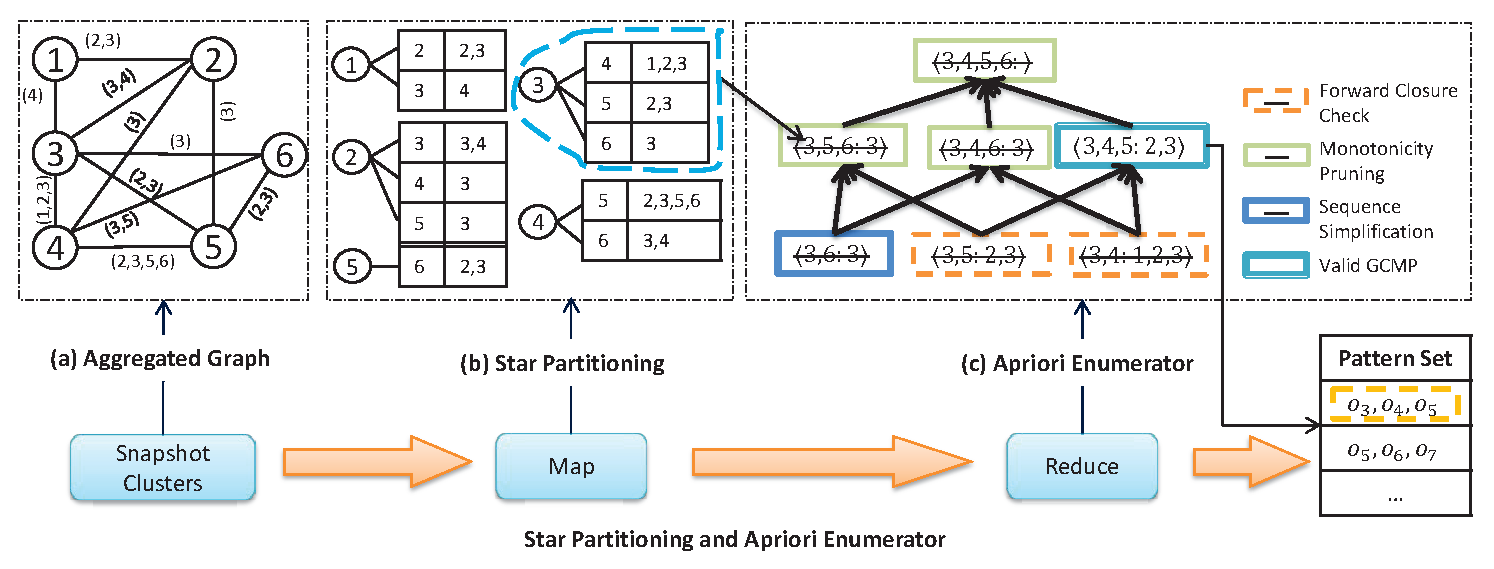
\includegraphics[width=\textwidth]{chapter5/spm.eps}
\caption{Star Partitioning and ApRiori Enumerator (SPARE). (a) Aggregated graph $G_A$ generated from Figure 1. (b) Five star partitions are generated from $G_A$. Star IDs are circled, vertexes and inverted lists are in the connected tables.
(c) Apriori Enumerator with various pruning techniques.}
\label{fig:star_partition}
%\vspace{-0.5em}
\end{figure*}

\section{SPARE: Star Partitioning and Apriori Enumerator}
\label{sec:spm}
The aforementioned TRPM scheme replicates snapshots based on the temporal dimension which suffers from two drawbacks. First, the replication factor $\eta$ can be large. Second, the same valid pattern may be redundantly discovered from different partitions.
To resolve these limitations,
we propose a new Star Partitioning and ApRiori Enumerator, named SPARE, 
to replace the second stage of the mapreduce jobs in Figure~\ref{fig:trm}. 
Our new parallel mining framework is shown in Figure~\ref{fig:star_partition}. 
Its input is the set of clusters generated in each snapshot and the output 
contains all the valid GCMPs. In the following, we explain the two major components: 
star partitioning and apriori enumerator.


\subsection{Star Partitioning}
Let $G_t$ be a graph for snapshot $S_t$, in which each node 
is a moving object and two objects are connected if they appear 
in the same cluster. It is obvious that $G_t$ consists of a set of small cliques. 
Based on $G_t$, we define an aggregated graph $G_A$ to summarize the 
cluster relationship among all the snapshots. In $G_A$, two objects
form an edge if they are connected in any $G_t$s. Furthermore, 
we attach an inverted list for each edge, 
storing the associated timestamps in which the two objects are connected. 
An example of $G_A$, built on the trajectory database in Figure~\ref{fig:related_work}, 
is shown in Figure~\ref{fig:star_partition} (a). 
As long as two objects are clustered in any timestamps, they are connected in $G_A$. 
The object pair $\langle o_1,o_2 \rangle$ appears in two clusters at timestamps 
$2$ and $3$ and is thus associated with an inverted list $(2,3)$.

We use \emph{star}~\cite{yoo2006joinless} as the data structure to capture the pair relationships. 
To avoid duplication, as $G_t$ is an undirected graph and an edge may appear in multiple stars, 
we enforce a global vertex ordering among the objects and propose a concept named \textit{directed star}.

\begin{definition}[Directed Star]
Given a vertex with global ID $s$, its directed star $Sr_s$ is defined as the set of neighboring vertexes with global ID $t>s$. We call $s$ the star ID.
\end{definition}

With the global vertex ordering, we can guarantee that each edge is contained in a unique star partition. Given the aggregated graph $G_A$  in Figure~\ref{fig:star_partition} (a), we enumerate all the possible directed stars in Figure~\ref{fig:star_partition} (b). These stars are emitted from mappers to different reducers. The key is the star ID and the value is the neighbors in the star as well as the associated inverted lists. 
The reducer will then call the Apriori-based algorithm to enumerate all the valid GCMPs.


Before we introduce the Apriori Enumerator, we are interested to 
examine the issue of global vertex ordering.
% on the moving objects.
This is because assigning different IDs to the objects will result in 
different star partitioning results, which will eventually affect the workload 
balance among reducers. The job with the performance bottleneck is often known as a  \emph{straggler}~\cite{kwon2012skewtune}. In the context of star partitioning, a straggler refers to the job assigned with the maximum star partition. We use $\Gamma$ to denote the size of such straggler partition and $\Gamma$ is set to the number of edges in a directed star\footnote{A star is essentially a tree structure and the number of nodes equals the number of edges minus one.}. Clearly, a star partitioning with small $\Gamma$ is preferred. For example, Figure~\ref{fig:star-alt} gives two star partitioning results under 
different vertex ordering on the same graph. The top one has $\Gamma = 5$ while the bottom one has $\Gamma = 3$. Obviously, the bottom one has a smaller $\Gamma$ and is much more balanced.

\begin{figure}[h]
\centering
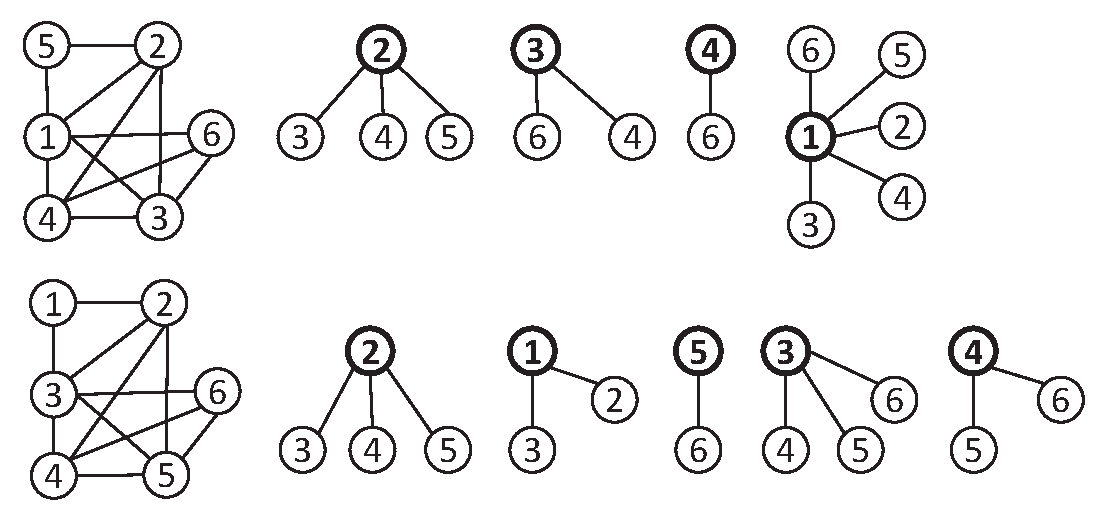
\includegraphics[width=0.8\textwidth]{chapter5/star-alt.eps}
\caption{Star partitioning with different vertex orderings.}
\label{fig:star-alt}
\end{figure}

Although it is very challenging to find the optimal vertex ordering from the $n!$ possibilities, we observe that a random order can actually achieve satisfactory performance based on the following theorem.


\begin{theorem}
\label{THM:SPM_LB}
Let $\Gamma^*$ be the value derived from the optimal vertex ordering and  $\Gamma$ be the value derived from a random vertex ordering. With probability $1-1/n$, we have $\Gamma = \Gamma^* + O(\sqrt{n \log n})$.
\end{theorem}
\begin{proof}
%\vspace{-0.5em}
See Appendix~\ref{apx:thm2proof}.
\end{proof}
If $G_A$ is dense, we are able to obtain a tighter bound for $(\Gamma - \Gamma^*)$.
\begin{theorem}
\label{THM:SPM_LB_INC}
Let $d$ be the average degree in $G_A$. If $d\geq \sqrt{12\log n}$, with
probability $1-1/n$, $\Gamma = \Gamma^* + O(\sqrt{d\log n})$.
\end{theorem}
\begin{proof}
%\vspace{-0.5em}
See Appendix~\ref{apx:thm2proof}.
\end{proof}
Hence, we can simply use object ID to determine the vertex ordering in our implementation.


\subsection{Apriori Enumerator}
Intuitively, given a GCMP with an object set $\{o_1,\ldots,o_m\}$, 
all the pairs of $\langle o_i,o_j \rangle$ with $1\leq i<j\leq m$ must 
be connected in the associated temporal graphs $\{G_t\}$. This inspires us to leverage the classic Apriori algorithm~\cite{agrawal1994fast} to enumerate all the valid GCMPs starting from pairs of objects. However, we observe that the monotonicity property does not hold between an object set and its supersets.

\begin{example}
In this example, we show that if an object set is not a valid pattern, we cannot prune all its super sets.
Consider two candidates $P_1=\langle o_1,o_2:1,2,3,6 \rangle$ and $P_2=\langle o_1,o_3:1,2,3,7 \rangle$. 
Let $L=2,K=3$ and $G=2$. Both candidates are not valid patterns because the constraint on $L$ is not satisfied. 
However, when considering their object superset $\langle o_1,o_2,o_3 \rangle$, we can infer that their co-clustering timestamps are in $(1,2,3)$. This is a valid pattern conforming to the constraints of $L,K,G$. Thus, we need a new type of monotonicity to facilitate pruning.
\end{example}   


\subsubsection{Monotonicity}
To ensure monotonicity, we first introduce a procedure named \textit{sequence simplification}, to reduce the number of edges as well as unnecessary timestamps in the inverted lists. For instance, if the size of the inverted list for an edge $e$ is smaller than $K$, then the edge can be safely removed because the number of timestamps in which its supersets are clustered must also be smaller than $K$. To generalize the idea, we propose three concepts: \textit{maximal $G$-connected subsequence}, \emph{decomposable sequence} and \emph{sequence simplification}.

\begin{definition}[Maximal $G$-connected Subsequence]
A sequence $T'$ is said to be a maximal $G$-connected subsequence of $T$ if (1) $T'$ is the subsequence of $T$, (2) $T'$ is $G$-connected, and (3) there exists no other subsequence $T''$ of $T$ such that $T'$ is the subsequence of $T''$ and $T''$ is G-connected.
\end{definition}

\begin{example}
Suppose $G=2$ and consider two sequences $T_1=(1,2,4,5,6,9,10$, $11,13)$ and $T_2=(1,2,4,5,6,8,9)$. $T_1$ has two maximal $2$-connected subsequences:$T_1^A=(1,2,4,5,6)$ and $T_1^B=(9,10,11,13)$. This is because the gap between $T_1^A$ and $T_1^B$ is $3$ and it is impossible for the timestamps from  $T_1^A$ and $T_1^B$ to form a new subsequence with $G\leq 2$. Since $T_2$ is $2$-connected, $T_2$ has only one maximal $2$-connected subsequence which is
itself. 
\end{example}

The maximal $G$-connected subsequence has the following two properties:
\begin{lemma}\label{lemma:union-property}
Suppose $\{T_1,T_2,\cdots,T_m\}$ is the set of all maximal $G$-connected subsequences of $T$, we have (1) $T_i\cap T_j=\emptyset$ for $i\neq j$ and (2) $T_1\cup T_2\cup\cdots\cup T_m=T$.
\end{lemma}
\begin{proof}
%\vspace{-0.5em}
We assume $T_i\cap T_j\neq \emptyset$ and prove (1) by contradiction. Let $T_i=(T_i[1], \cdots,T_i[p])$ and $T_j= (T_j[1], \cdots,T_j[n])$. Suppose $T[x]$ is a timestamp occurring in both $T_i$ and $T_j$. Let $T[y]=\min\{T_i[1],T_j[1]\}$, i.e., the minimum timestamp of $T_i[1]$ and $T_j[1]$ occurs at the $y$-th position of sequence $T$. Similarly, we assume $T[z]=\max\{T_i[p], T_j[n]\}$. Apparently, the two subsequences $T[y:x]$ and $T[x:z]$ are $G$-connected because $T_i$ and $T_j$ are both $G$-connected. Then, sequence $(T_y,\cdots,T_x,\cdots,T_z)$, the superset of $T_i$ and $T_j$, is also $G$-connected. This contradicts with the assumptions that $T_i$ and $T_j$ are maximal $G$-connected subsequences. 

To prove (2), we assume $\cup_{i=1}^{i=m} T_i$ does not cover all the timestamps in $T$. Then, we can find a subsequence $T'=T[x:x+t]$ such that $T[x-1]\in T_a$ $(1\leq a\leq m)$, $T[x+t+1]\in T_b$ $(1\leq b\leq m)$ and all the timestamps in $T'$ is not included in any $T_i$. Let $g'=\min\{T[x]-T[x-1], T[x+t+1]-T[x+t]\}$. If $g'\leq G$, then it is easy to infer that $T_a$ or $T_b$ is not a maximal $G$-connected subsequence because we can combine it with $T[x]$ or $T[x+t]$  to form a superset which is also $G$-connected. If $g'>G$, $T'$ itself is a maximal $G$-connected subsequence which is missed in $\cup_{i=1}^{i=m} T_i$. Both cases lead to contradictions.
\end{proof}




\begin{lemma}\label{lemma:subset-property}
%If $T_1$ is a subset of $T_2$, 
If $T_1 \subseteq T_2$, then for any maximal $G$-connected subsequence $T_1'$ of $T_1$, we can find a maximal $G$-connected subsequence $T_2'$ of $T_2$ such that %$T_1'$ is a subset of $T_2'$.
$T_1' \subseteq T_2'$.
\end{lemma}
\begin{proof}
%\vspace{-0.5em}
Since $T_1' \subseteq T_1 \subseteq T_2 $, we know $T_1'$ is a $G$-connected subsequence of $T_2$. Based on Lemma~\ref{lemma:union-property}, we can find a maximal $G$-connected subsequence of $T_2$, denoted by $T_2'$, such that $T_1'\cap T_2'\neq \emptyset$. If there exists a timestamp $T_1'[x]$ such that $T_1'[x]\notin T_2'$, similar to the proof of case (1) in Lemma~\ref{lemma:union-property}, we can obtain a contradiction. Thus, all the timestamps in $T_1'$ must occur in $T_2'$.
\end{proof}

\begin{definition}[Decomposable Sequence]
$T$ is decomposable if for any of its maximal $G$-connected subsequence $T'$, we have (1) $T'$ is $L$-consecutive; and (2) $|T'|\geq K$.
\end{definition}

\begin{example}
Let $L = 2, K = 4$ and we follow the above example. $T_1$ is not a decomposable sequence
because one of its maximal $2$-connected subsequence (i.e., $T_1^B$) is not $2$-consecutive.
In contrast, $T_2$ is a decomposable sequence because the sequence itself is the maximal $2$-connected subsequence, which is also $2$-consecutive and with size  $\geq 4$.
\end{example}

\begin{definition}[Sequence Simplification]
Given a sequence $T$, the simplification procedure $\mathtt{sim}(T) =  g_{G,K} \cdot f_L(T) $ can be seen as a composite function with two steps: 
\begin{enumerate}
\item $f$-step: remove segments of $T$ that are not $L$-consecutive;
\item $g$-step: among the maximal $G$-connected subsequences of $f_L(T)$, remove those with size smaller than $K$.
\end{enumerate}
\end{definition}


\begin{example}
Take $T=(1,2,4,5,6,9,10,11,13)$ as an example for sequence simplification. 
Let $L = 2, K = 4$ and $G = 2$. In the $f$-step, $T$ is reduced to $f_2(T)=(1,2,4,5,6,9,10,11)$. 
The segment $(13)$ is removed due to the constraint of $L=2$. 
$f_2(T)$ has two maximal $2$-consecutive subsequences: $(1,2,4,5,6)$ and $(9,10,11)$. 
Since $K=4$, we will remove $(9,10,11)$ in the $g$-step. Finally, the output is $\mathtt{sim}(T)=(1,2,4,5,6)$.
\end{example}

It is possible that the simplified sequence $\mathtt{sim}(T)=\emptyset$. For example, Let $T=(1,2,5,6)$ 
and $L=3$. All the segments will be removed in the $f$-step and the output is $\emptyset$.
We define $\emptyset$ to be not decomposable. 
%Based on the above definitions, we can define our monotonicity to facilitate the pruning in the Apriori algorithm.
We then link \emph{sequence simplification} and \emph{decomposable sequence} in the following lemma:
%We provide an important property of the sequence simplification process as follows:
\begin{lemma}\label{lemma:decom-sim}
If sequence $T$ is a superset of any decomposable sequence, then $\mathtt{sim}(T) \neq \emptyset$.
\end{lemma}

\begin{proof}
%\vspace{-0.5em}
It is obvious that $\mathtt{sim}(T)$ is a one-to-one function. Given an input sequence T, there is a unique  $\mathtt{sim}(T)$. Let $T_p$ be a decomposable subset of $T$ and we prove the lemma by showing that $\mathtt{sim}(T)$ is a superset of $T_p$.

Suppose $T_p$ can be decomposed into a set of maximal $G$-connected
subsequences $T_p^1, \ldots, T_p^m$ ($m \geq 1$). Since $T_p$ is a subset of $T$, all the $T_p^i$ are also subsets of $T$. By definition, each $T_p^i$ is $L$-consecutive. Thus, in the $f$-step of $\mathtt{sim}(T)$, none of $T_p^i$ will be removed. In the $g$-step, based on Lemma~\ref{lemma:subset-property}, we know that each $T_p^i$ has a superset in the maximal $G$-connected subsequences of $f_L(T)$. Since $|T_p^i|\geq K$, none of $T_p^i$ will be removed in the $g$-step. Therefore, all the $T_p^i$ will be retained after the simplification process and $\mathtt{sim}(T) \neq \emptyset$.
\end{proof}

With Lemma~\ref{lemma:decom-sim}, we are ready to define the \emph{monotonicity} concept based on the simplified
sequences to facilitate the pruning in the Apriori algorithm. 

\begin{theorem}[Monotonicity]\label{THM:SPARE_MONO}
Given a candidate pattern $P=\{O:T\}$, if $\mathtt{sim}(P.T)=\emptyset$, then any pattern candidate $P'$ with $P.O \subseteq P'.O$ can be pruned.
\end{theorem}

\begin{proof}
%\vspace{-0.5em}
We prove by contradiction. Suppose there exists a valid pattern $P_2$ such that $P_2.O \supseteq P.O$. It is obvious that $P_2.T \subseteq P.T$. Based on Definition 2, the following conditions hold: (1) $P_2.T$ is $G$-connected. (2) $|P_2.T| \geq K$ and (3) $P_2.T$ is $L$-consecutive. Note that the entire $P_2.T$ is $G$-connected. Thus, $P_2.T$ itself is the only maximal $G$-connected subsequence. Based on conditions (1),(2),(3) and Definition 6, $P_2.T$ is decomposable. Then, based on Lemma~\ref{lemma:decom-sim}, we know $\mathtt{sim}(T)\neq \emptyset$ because $P_2.T \subseteq P.T$ and $P_2.T$ is decomposable. This contradicts with $\mathtt{sim}(P.T)=\emptyset$.
\end{proof}

\subsubsection{Apriori Enumerator}
We design an Apriori based enumeration algorithm to efficiently discover all the valid patterns in a star partition. The principle of the Apriori algorithm is to construct a lattice structure and enumerate all the possible candidate sets in a bottom-up manner. Its merit lies in the monotonic property such that if a candidate set is not valid, then all its supersets can be pruned. Thus, it works well in practice in spite of the exponential search space.

Our customized Apriori Enumerator is presented in Algorithm~\ref{algo:apriori_mining}. Initially, the edges (pairs of objects) in the star constitute the bottom level (Lines~\ref{code:init-start}-\ref{code:init-end}) and invalid candidates are excluded (Line~\ref{code:simp1}). An indicator \emph{level} is used to control the result size for candidate joins. During each iteration (Lines~\ref{code:level-start}-\ref{code:level-ends}), only candidates with object size equals to \emph{level} are generated (Line~\ref{code:join-start}). When two candidates $c_1$ and $c_2$ are joined, the new candidate becomes $c'=\langle c_1.O \cup c_2.O, c_1.T\cap c_2.T\rangle$ (Line~\ref{code:join}). To check the validity of the candidate, we calculate $\mathtt{sim}(c'.T)$. If its simplified sequence is empty, $c'$ is excluded from the next level (Line~\ref{code:simp2}). This ensures that all the candidates with $P.O\supseteq c'.O$ are pruned. If a candidate cannot generate any new candidate, then
it is directly reported (Lines~\ref{code:output1-start}-\ref{code:output1-end}).
To further improve the performance, we adopt the idea of \textit{forward closure}~\cite{wang2003closet+,pei2000closet} and  aggressively check if the union of all the current candidates form a valid pattern (Lines~\ref{code:fc-checking-start}-\ref{code:fc-checking-end}). If yes, we can  terminate the algorithm early and output the results.

\begin{algorithm}[h]
\caption{Apriori Enumerator}
\label{algo:apriori_mining}
\begin{algorithmic}[1]
\Require{$Sr_s$}
\State {$C \leftarrow \emptyset$}
\ForAll{edges $c=\langle o_i\cup o_j, T_{o_i}\cap T_{o_j}\rangle$ in $Sr_s$} \label{code:init-start}
\If {$\mathtt{sim}(T_{o_i}\cap T_{o_j})\neq \emptyset$}
\State {$C\leftarrow C\cup \{c\}$} \label{code:simp1}
\EndIf 
\EndFor\label{code:init-end}
\State $\mathrm{level} \gets 2$ \label{code:level}
\While{$C\neq \emptyset$} \label{code:level-start}
	\ForAll{$c_1 \in C$}
		\ForAll{$c_2 \in C$ and $|c_2.O \cup c_2.O| = \mathrm{level}$}\label{code:join-start}	
			\State {$c' \gets \langle c_1.O \cup c_2.O:(c_1.T \cap c_2.T )\rangle$} \label{code:join}			
			\If{ $\mathtt{sim}(c'.T)\neq \emptyset$} \label{code:simp2}
					\State {$C'\leftarrow C'\cup \{c'\}$}
			\EndIf			
		\EndFor\label{code:join-end}
		\If {no $c'$ is added to $C'$} \label{code:output1-start}
			\If{$c_1$ is a valid pattern}
				\State output $c_1$
			\EndIf
		\EndIf \label{code:output1-end}
	\EndFor
	\State $O_u \gets $ union of $c.O$ in $C$	\label{code:fc-checking-start}
	\State $T_u \gets $ intersection of $c.T$ in $C$	
	\If {$\langle O_u, T_u\rangle$ is a valid pattern}
		\State{output $\langle O_u, T_u\rangle$, \textbf{break}} \label{code:fc-checking}
	\EndIf \label{code:fc-checking-end}
	\State {$C\leftarrow C';C'\leftarrow \emptyset; \mathrm{level} \gets \mathrm{level}+1$}	
\EndWhile\label{code:level-ends}
\State output $C$ \label{code:output2-end}
\end{algorithmic}
\end{algorithm}



\begin{example}
As shown in Figure~\ref{fig:star_partition} (c), in the bottom level of the lattice structure, candidate $\langle 3,6:3 \rangle $ is pruned because its simplified sequence is empty. Thus, all the object sets containing $\langle 3,6 \rangle $ can be pruned. The remaining two candidates (i.e., $\langle 3,4:1,2,3 \rangle$ and $\langle 3,5:2,3 \rangle$)  derive a new  $\langle 3,4,5:2,3 \rangle$ which is valid. By the forward closure checking, the algorithm can terminate and output $\langle 3,4,5:2,3 \rangle$ as the final pattern.
\end{example}


\subsection{Put Everything Together}
We summarize the workflow of SPARE in Figure~\ref{fig:star_partition} as follows. After the parallel clustering in each snapshot, for ease of presentation, we use an aggregated graph $G_A$ to capture the clustering relationship. However, in the implementation of the map phase, there is no need to create $G_A$ in advance. Instead, we simply need to emit the edges within a star to the same reducer. 
%Before sending stars to reducers, we use a simple best-fit strategy to calculate the star allocation. Under the best-fit strategy, the most costly unallocated star is assigned to the most lightly loaded reducers, where we use the edges in the star as a cost estimation.
Each reducer is an Apriori Enumerator. When receiving a star $Sr_i$, the reducer creates initial candidate patterns. Specifically, for each $o \in Sr_i$, a candidate pattern $\langle o,i: e(o,i) \rangle$ is created. Then it enumerates all the valid patterns from the candidate patterns. The pseudocode of SPARE is presented in Algorithm~\ref{algo:spm_overview}. 
In our implementation of SPARE on Spark~\cite{zaharia2012resilient}, we take advantage of Spark features to achieve better workload balance. In particular,
we utilize Spark DAG execution engine to inject a planning phase between map and reduce phases. By knowing all map results (i.e., star sizes), a simple best-fit strategy is adopted which assigns the most costly unallocated star to the most lightly loaded reducer, where the edges in a star are used as cost estimations. We also leverage Spark in-memory cache to avoid recomputing all stars after the planning phase.
% 
%In Apache Spark, further optimization can be made by balancing the loads among reducers at runtime. 
%Leveraging
%Spark's DAG execution engine~\cite{zaharia2012resilient}, a planning phase can be inserted in between map and reduce phases.
%With knowing all map results (i.e., star sizes), a simple best-fit planning strategy can be adopted by assigning the most costly unallocated star to the most lightly loaded reducer, where the edges in a star can be used as a cost estimation.

\begin{algorithm}
\caption{Star Partitioning and ApRiori Enumerator}
\label{algo:spm_overview}
\begin{algorithmic}[1]
\Require list of $\langle t, S_t \rangle$ pairs
\State {\textit{---Map phase---}}
\label{code:spm-map-start}
\ForAll{$C \in S_t$}
	\ForAll {$o_1 \in C,  o_2 \in C, o_1 < o_2$}
	\State emit a $\langle o_1, o_2, \{t\}\rangle$ triplet~\label{code:spm-edge-direct}
	\EndFor
\EndFor
\label{code:spm-map-end}

\State {\textit{---Partition and Shuffle phase---}}
\label{code:spm-shuffle-start}
\ForAll{$\langle o_1, o_2, \{t\}\rangle$ triplets} 
	\State group-by $o_1$, emit $\langle o_1, Sr_{o_1} \rangle$ 
\EndFor
\label{code:spm-shuffle-end}

\State {\textit{---Reduce phase---}}
\label{code:spm-reduce-start}
\ForAll{$\langle o, Sr_{o} \rangle$}
\State call Apriori Enumerator for star $Sr_o$
\EndFor
\label{code:spm-reduce-end}

\end{algorithmic}
\end{algorithm}

Compared with TRPM, the SPARE framework does not rely on snapshot replication to guarantee correctness. In addition, we can show that the patterns derived from a star partition are unique and there would not be duplicate patterns mined from different star partitions.
\begin{theorem}[Pattern Uniqueness]
\label{LEM:SPM_CORRECT}
Let $Sr_i$ and $Sr_j$ ($i\neq j$) be two star partitions. Let $P_i$ (resp. $P_j$) be 
the patterns discovered from $Sr_i$ (resp. $Sr_j$). 
Then, $\forall p_i \in P_i, \forall p_j \in P_j$, we have $p_i.O \neq p_j.O$.
\end{theorem}
\begin{proof} 
%\vspace{-0.5em}
We prove by contradiction. Suppose there exist $p_i \in P_i$ and $p_j \in P_j$ with the same object set. Note that the center vertex of the star is associated with the minimum id. Let $o_i$ and $o_j$ be the center vertexes of the two partitions and we have $o_i=o_j$. However, $P_i$ and $P_j$ are from different stars, meaning their center vertexes are different (i.e., $o_i\neq o_j$), leading to a contradiction. 
%\vspace{-0.5em}
\end{proof}

Theorem~\ref{LEM:SPM_CORRECT} implies that no mining efforts are wasted in discovering redundant patterns  
%that no replication is required 
in the SPARE framework, which is superior to the TRPM baseline. Finally, we show the correctness of the SPARE framework.
\begin{theorem}
\label{THM:SPM_CORRECT}
The SPARE framework guarantees completeness and soundness.
\end{theorem}
\begin{proof}  
%\vspace{-0.5em}
See Appendix~\ref{apx:spm_correct}.
%\vspace{-0.5em}
\end{proof}

\section{Experimental Evaluation}\label{gw:sec:exp}
In this section, we present a comprehensive experimental evaluation 
of our solutions using several real-world information networks and 
various synthetic datasets. 
%Since the focus of this chapter is on query efficiency, we do not evaluate the efficiency of index updates. 
All experiments are conducted on an 
Amazon EC2 r3.2xlarge machine\footnote{http://aws.amazon.com/ec2/pricing/}, 
with an 8-core 2.5GHz CPU, 60GB memory and 320GB hard drive 
running with 64-bit Ubuntu 12.04. As the source code of EAGR is not
available, we implemented it and used it as a reference in our comparative
study.  
All algorithms are implemented in Java and run under JRE 1.6.

\begin{table}[h]
\caption{Large-scale real graphs.}
\label{tab:realdata}
\centering
\begin{tabular}{|l|l|l|l|}
\hline 
\rule[-1ex]{0pt}{2.5ex} Name & Type & Number of Vertexes & Number of Edges \\ 
\hline 
\rule[-1ex]{0pt}{2.5ex} LiveJournal1 & undirected & 3,997,962 & 34,681,189 \\ 
\hline 
\rule[-1ex]{0pt}{2.5ex} Pokec & directed & 1,632,803 & 30,622,564 \\ 
\hline 
\rule[-1ex]{0pt}{2.5ex} Orkut & undirected & 3,072,441 & 117,185,083 \\ 
\hline 
\rule[-1ex]{0pt}{2.5ex} DBLP & undirected & 317,080 & 1,049,866 \\ 
\hline 
\rule[-1ex]{0pt}{2.5ex} YouTube & undirected & 1,134,890 & 2,987,624 \\ 
\hline 
\rule[-1ex]{0pt}{2.5ex} Google & directed & 875,713 & 5,105,039 \\ 
\hline 
\rule[-1ex]{0pt}{2.5ex} Amazon & undirected & 334,863 & 925,872 \\ 
\hline 
\rule[-1ex]{0pt}{2.5ex} Stanford-web & directed & 281,903 &  2,312,497 \\ 
\hline 
\end{tabular}
\end{table}


\textbf{Datasets.} For real datasets, we use 8 information networks 
which are available at the Stanford \emph{SNAP}\footnote{http://snap.stanford.edu/snap/index.html}: 
LiveJournal1, Pokec, Orkut, DBLP, YouTube, Google, Amazon and Stanford-web. 
The detail description of these datasets is provided in 
Table~\ref{tab:realdata}. 

For synthetic datasets, we use two widely used graph data generators. 
We use the \emph{DAGGER} generator \cite{yildirim2013dagger} to generate 
all the synthetic DAGs and the SNAP graph data generator at the
Stanford SNAP website to generate non-DAG datasets. For each dataset, each vertex is associated with an integer attribute.

\textbf{Query.} In all the experiments, the window query is conducted 
by using the SUM() as the aggregate function over the integer attribute in each dataset. 

\begin{figure*}[t]
\centering
\begin{subfigure}{0.45\textwidth}
  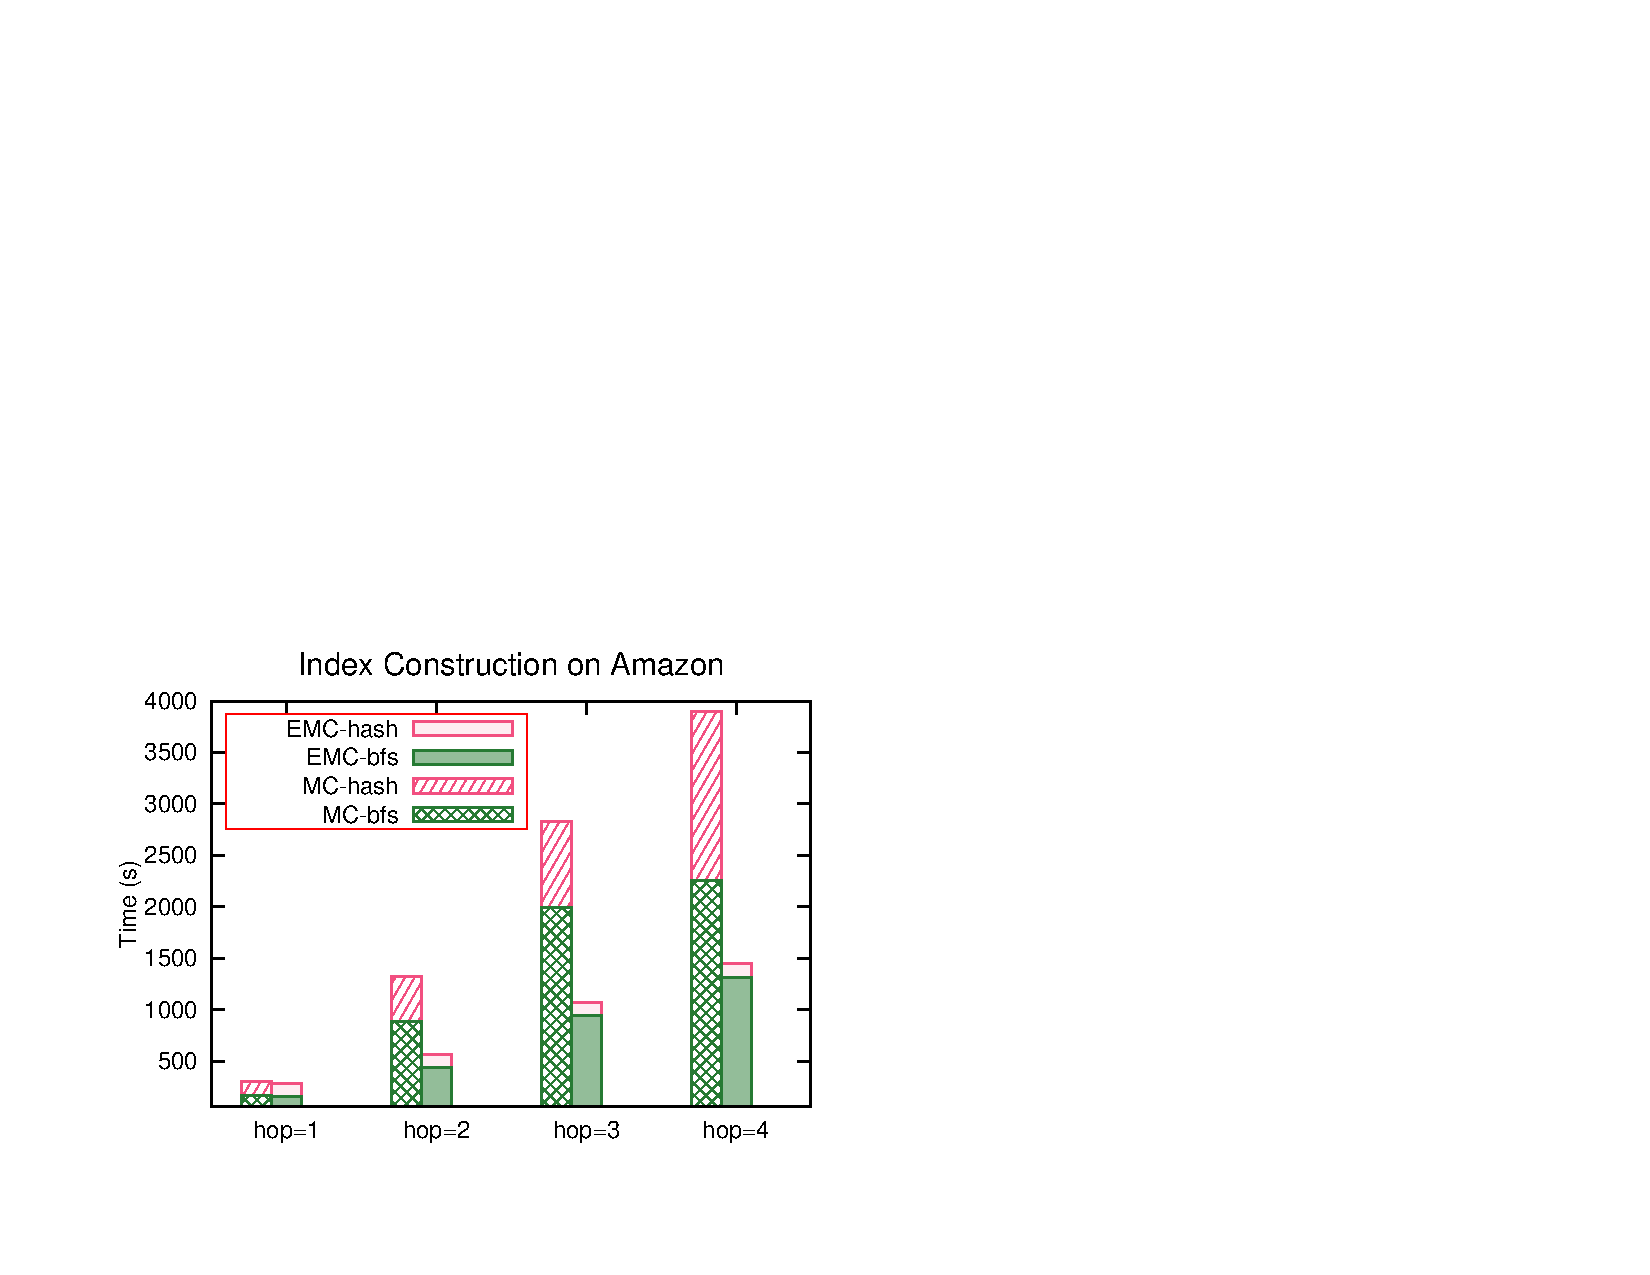
\includegraphics[width=\textwidth]{chapter3/exp/khopeffect/effectiveness/amazon_index_time.pdf}
  \caption{Index built on Amazon}
\end{subfigure}
\begin{subfigure}{0.45\textwidth}
  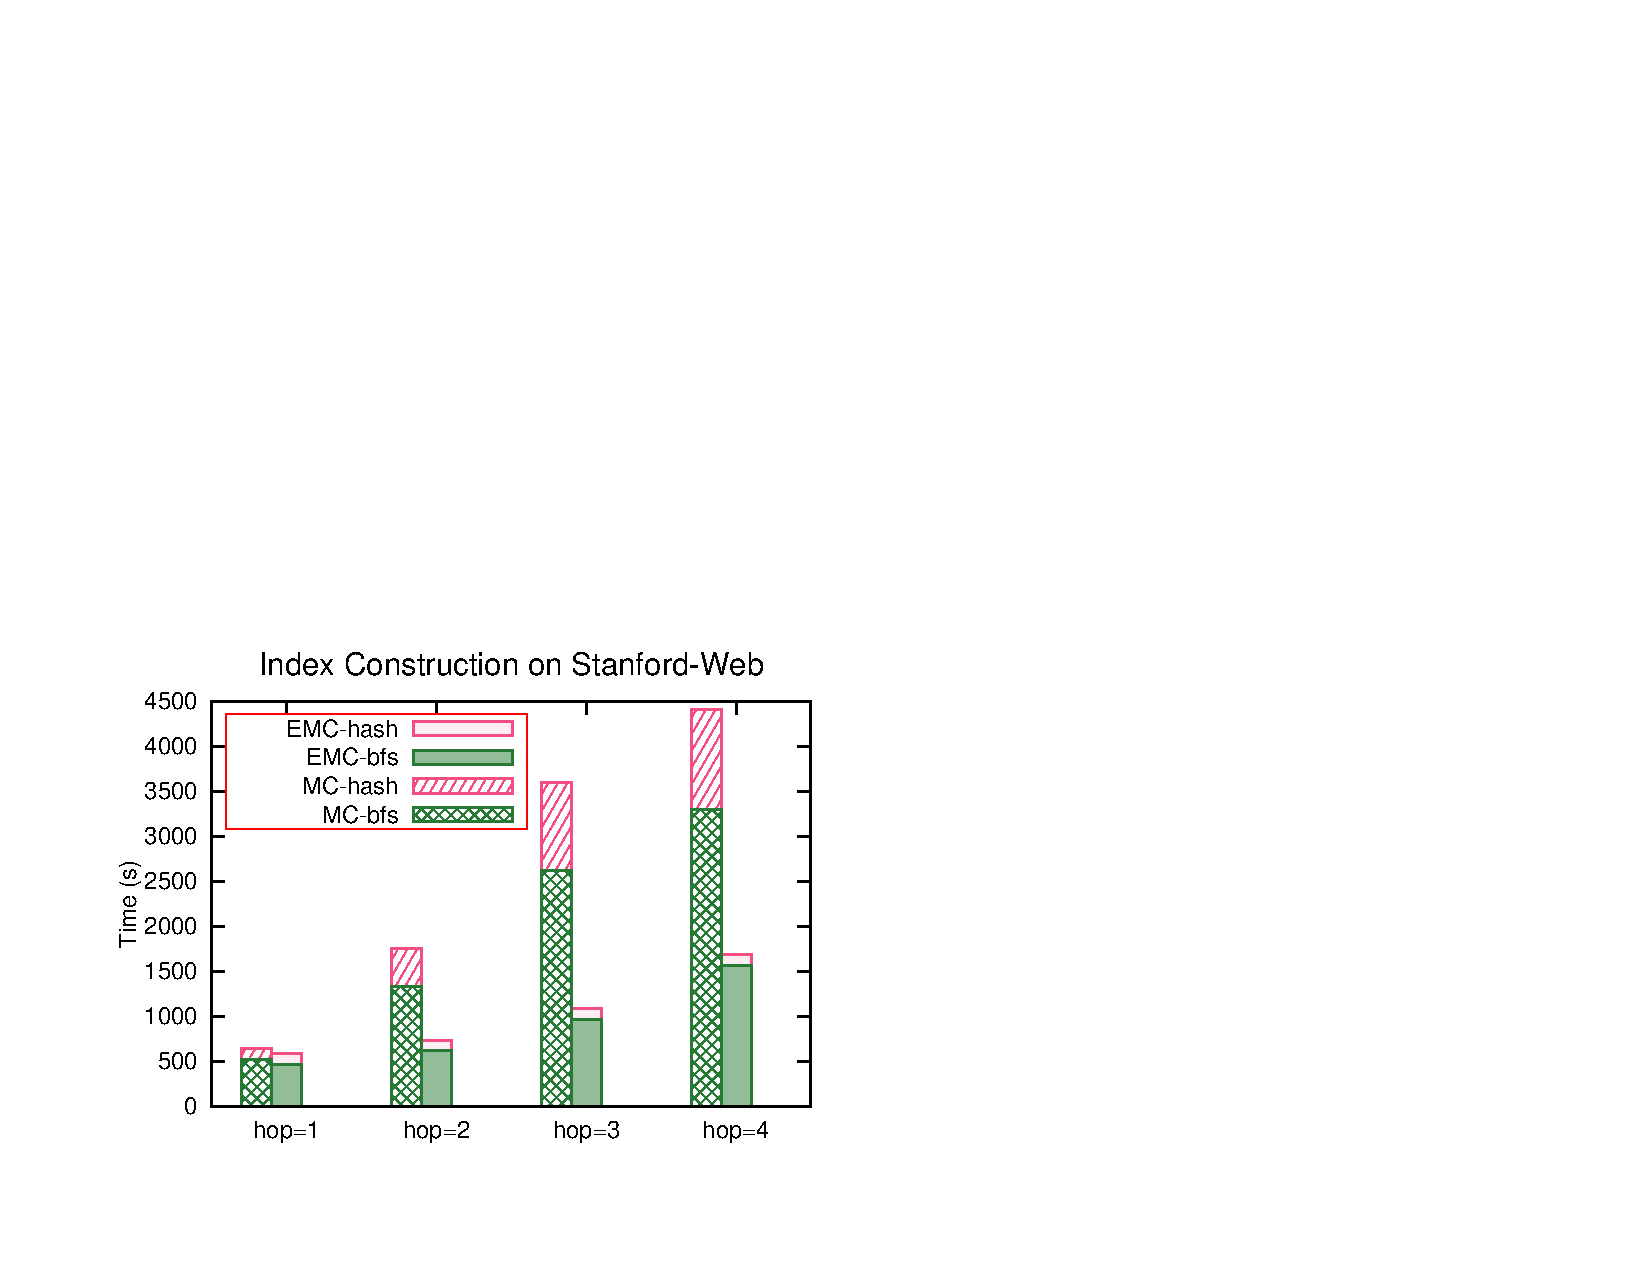
\includegraphics[width=\textwidth]{chapter3/exp/khopeffect/effectiveness/stanford_index_time.pdf}
  \caption{Index built on Stanford-web}
\end{subfigure}

\begin{subfigure}{0.45\textwidth}
  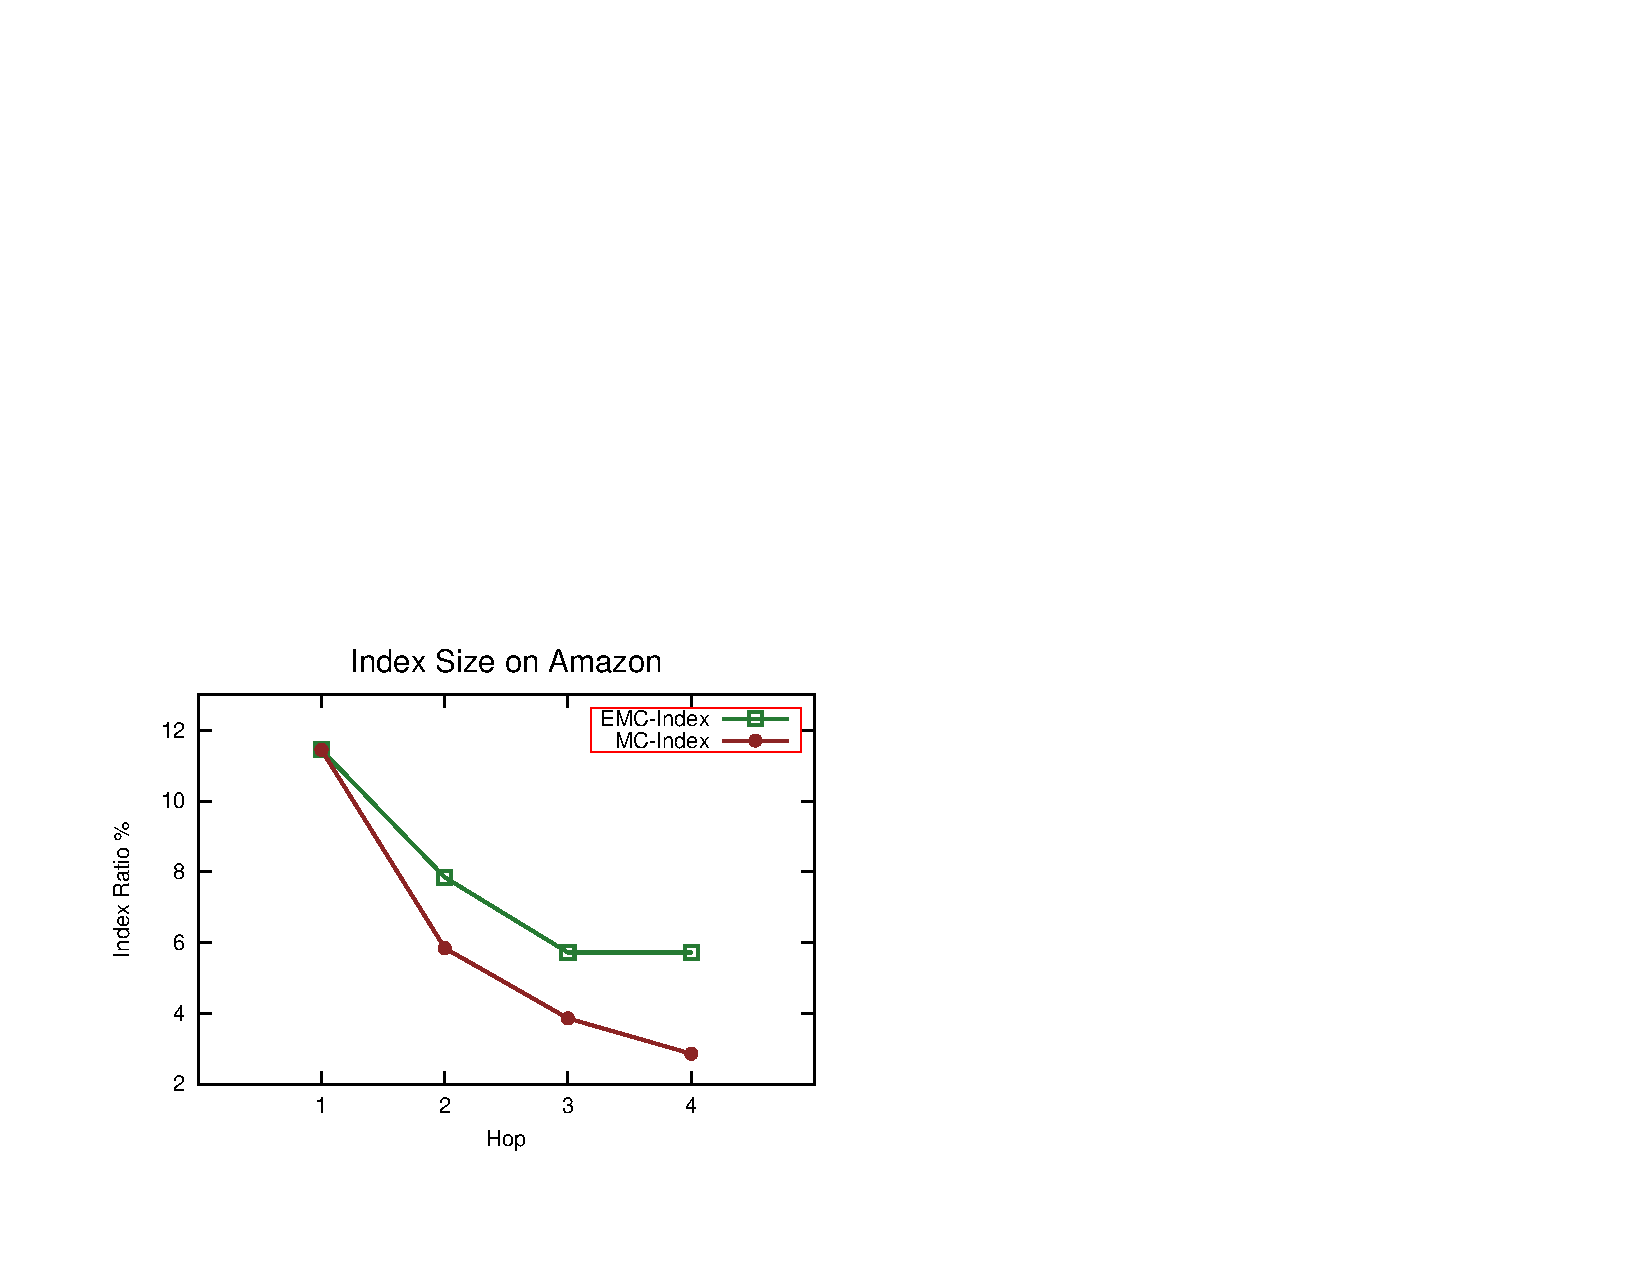
\includegraphics[width=\textwidth]{chapter3/exp/khopeffect/effectiveness/amazon_index_size.pdf}
  \caption{Index size on Amazon}
\end{subfigure}
\begin{subfigure}{0.45\textwidth}
  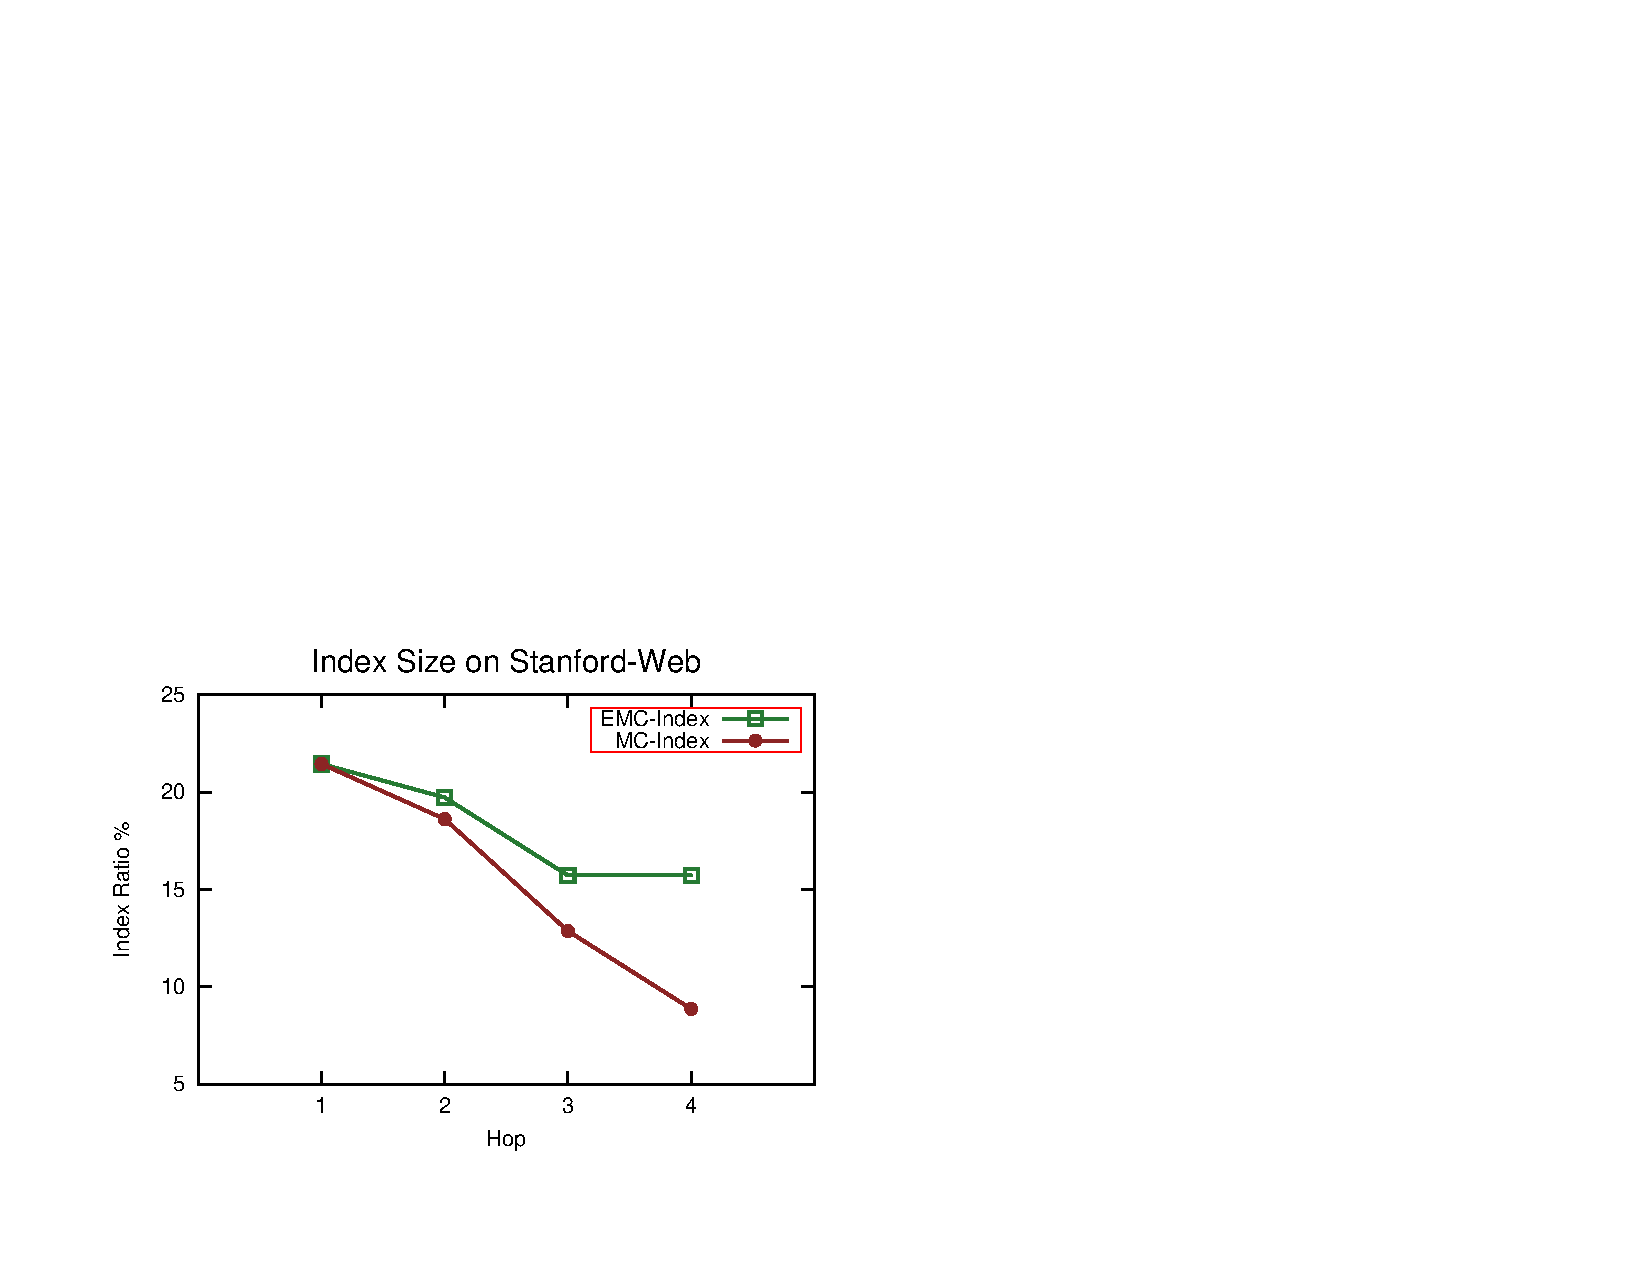
\includegraphics[width=\textwidth]{chapter3/exp/khopeffect/effectiveness/stanford_index_size.pdf}
  \caption{Index size on Stanford-web}
\end{subfigure}
\caption{Index construction analysis for EMC and MC. (a) and (b) 
depict the index time for the Amazon and Stanford-web networks.
(c) and (d) show the index size for the Amazon and Stanford-web datasets.}
\label{fig:index_analysis_emc_mc}
\end{figure*}


\subsection{Comparison between MC and EMC}\label{sec:mc_vs_emc}
We first compare the effectiveness of the two DBIndex 
construction algorithms: MinHash Clustering (MC) and Estimated 
MinHash Clustering (EMC). We look at 
the index construction time, index size and query performance. 
All these experiments are conducted based on two real datasets: 
Amazon and Stanford-web. For both datasets, we run a series of k-hop queries.\footnote{For the Stanford-web graph, which is directed,
the k-hop windows are directed k-hop windows where $u \in W(k)$ if there is a directed path
of at most $k$ hops from vertex $v$ to vertex $u$.
} For queries with hop count larger than 1, 
EMC uses 1-hop information for the initial clustering. 

\textbf{Index Construction. } Figures~\ref{fig:index_analysis_emc_mc} 
(a) and (b) compare the index construction time between MC and EMC 
when we vary the windows from 1-hop to 4-hop for the Amazon and Stanford-web 
graphs respectively. To better understand the time differences, 
the construction time is split into two parts: 
the MinHash cost (EMC-hash or MC-hash) and the breadth-first-search traversal (to compute the $k$-hop window)  cost (EMC-bfs or MC-bfs). The results show the same trend 
for the two datasets. % We make several observations.
First, as the number of hops increases, the index construction time increases as well. 
This is expected as a larger hop count results in a larger window size 
and the BFS and the MinHash time increase correspondingly. 
Second, as the hop count increases, the difference between the
index construction time of EMC and that of MC widens. 
For instance, as shown in Figures~\ref{fig:index_analysis_emc_mc} (a) and (b), for the 4-hop window queries, compared to MC, 
EMC can save $62\%$ and $66\%$ construction time for the Amazon and Stanford-Web datasets respectively.
EMC benefits from both the low MinHash cost and low BFS cost. 
%From Figures~\ref{fig:index_analysis_emc_mc} (a) and (b), 
We can also see that the MinHash cost of MC increases as the number of hops 
increases, while that for EMC remains almost the same as the 1-hop case. 
This shows that the cost of MinHash becomes more significant for larger windows. 
Thus, using 1-hop clustering for larger hop counts reduces the MinHash cost 
in EMC. Similarly, as EMC saves on BFS cost for $k$-hop queries where $k > 1$, 
the BFS cost of EMC is much smaller than that of MC as well. 

\textbf{Index Size.} Figures~\ref{fig:index_analysis_emc_mc} (c) and (d) 
present the effect of hop counts on the index size for the Amazon and Stanford-web 
datasets respectively. The y-axis shows the index ratio which is the index size over the original graph size. 
The insights derived are: 
First, the index size is rather small compared to the original graph: it
varies from $3\%$ to $12\%$ of the original graph for the Amazon dataset 
and from $8\%$ to $22\%$ for the Stanford-web dataset. 
Second, the index size decreases as the number of hops increases. 
While this appears counter-intuitive initially, it is actually reasonable: a larger hop results in a bigger window, which leads
to more dense blocks. Third, the index ratio of EMC is slightly larger 
than that of MC for larger hop count. This indicates that MC can find more dense blocks 
than EMC to reduce the index size. Fourth, the index ratio on 
the Amazon dataset is much smaller than the ones on the Stanford-web dataset. 
This is because the Amazon dataset is undirected while the Stanford-web dataset
is directed. For the Stanford-web dataset, since we use directed k-hop windows, the window size is naturally smaller. 

\begin{figure}[h]
\centering
\begin{subfigure}{0.48\linewidth}
\centering
  \includegraphics[width=\textwidth]{chapter3/exp/khopeffect/effectiveness/amazon_query_time.pdf}
  \caption{Amazon graph}
\end{subfigure}%
\begin{subfigure}{0.48\linewidth}
\centering
  \includegraphics[width=\textwidth]{chapter3/exp/khopeffect/effectiveness/stanford_query_time.pdf}
  \caption{Stanford-web graph}
\end{subfigure}
\caption{Query performance comparison of MC and EMC.}
\label{fig:khop_effective_query_time}
\end{figure}

\textbf{Query Performance.}       
Figures~\ref{fig:khop_effective_query_time} (a) and (b)
present the query time of MC and EMC 
on the two datasets respectively 
as we vary the number of hops from 1 to 4.
To appreciate the benefits of an index-based scheme, we also implemented
a \emph{Non-indexed} algorithm which computes window aggregate by performing $k$-bounded breadth
first search for each vertex individually in run time.
In Figures~\ref{fig:khop_effective_query_time} (a) and (b),
the execution time shown on the y-axis is in log scale. The results show that the index-based 
schemes outperform the non-index approach by four orders of magnitude. 
For instance, for the 4-hop query over the Amazon graph, 
our algorithm is 13,000 times faster than the non-index approach. 
This confirms that it is necessary to have well-designed index support 
for efficient window query processing. By utilizing DBIndex, 
for these graphs with millions of edges, every aggregation query 
can be processed in just between 30ms to 100ms for the Amazon graph and 
between 60ms to 360ms for the Stanford-web graph. In addition, we can 
see that as the number of hops increases, the query time decreases. 
This is the case because a larger hop count eventually results in a larger
number of dense blocks where more (shared) computation can be salvaged. 
Furthermore, we can see that the query time of EMC is slightly longer 
than that of MC when the number of hops is large. This is expected as 
EMC does not cluster based on the complete window information; instead, it
uses only partial information derived from the 1-hop windows. 
However, the performance difference is quite small even for 4-hop queries: for
the Amazon dataset, the difference is only 20ms; and for the Stanford-web
graph, the difference is 35ms. 
For small number of hops, the time difference is even smaller. 
This performance penalty is acceptable as tens of milliseconds time 
difference will not affect user's experience.  As EMC is significantly more 
efficient than MC in index construction, EMC may still be a 
promising solution to many applications. As such, 
in the following sections, we adopt EMC for DBIndex in
our experimental evaluations.  
 

\subsection{Comparison between DBIndex and EAGR}

In this set of experiments, we compare DBIndex and 
EAGR \cite{mondal2014eagr} using both large-scale real 
and synthetic datasets. As described in~\cite{mondal2014eagr},
for each dataset, EAGR runs for 10 
iterations in the index construction.

\begin{figure}[h]
\centering
\begin{subfigure}{0.45\linewidth}
  \centering
  \includegraphics[width=\textwidth]{chapter3/exp/khopeffect/real_data/real_index_time_h1.pdf}
  \caption{1-hop index construction}
\end{subfigure} \begin{subfigure}{0.45\linewidth}
  \centering
  \includegraphics[width=\textwidth]{chapter3/exp/khopeffect/real_data/real_query_time_h1.pdf}
  \caption{1-hop query performance}
\end{subfigure}%
\caption{Comparison between DBIndex and EAGR  for 1-hop query.}
\label{fig:1-hop-real}
\end{figure}

\begin{figure}[h]
\centering
\begin{subfigure}{0.45\linewidth}
  \centering
  \includegraphics[width=\textwidth]{chapter3/exp/khopeffect/real_data/real_index_time_h2.pdf}
  \caption{2-hop index construction}
\end{subfigure}
\begin{subfigure}{0.45\linewidth}
  \centering
  \includegraphics[width=\textwidth]{chapter3/exp/khopeffect/real_data/real_query_time_h2.pdf}
  \caption{2-hop query performance}
\end{subfigure}
\caption{Comparison between DBIndex and EAGR for 2-hop query.}
\label{fig:2-hop-real}
\end{figure}

\subsubsection{Real Datasets} 
We first study the index construction and 
query time performance of DBIndex and EAGR for 1-hop and 2-hop windows 
using 6 real datasets: DBLP, Youtube, Livejournal, Google, Pokec and Orkut. 
The results for 1-hop window and 2-hop window are presented
in Figures~\ref{fig:1-hop-real} and~\ref{fig:2-hop-real} 
respectively. 
As shown in Figures~\ref{fig:1-hop-real}(a) and~\ref{fig:2-hop-real}(a), both DBIndex and EAGR can build the index for all
the real datasets for the 1-hop but EAGR runs out of the memory for the 2-hop query on LiveJournal and Orkut datasets. This further confirms that EAGR incurs 
high memory usage as it needs to build the FP-Tree and 
maintain the vertex-window mapping information. We also observe that 
DBIndex is significantly faster than EAGR in index creation. 
We emphasize that the time is shown in logarithmic scale. 
For instance, for Orkut dataset, EAGR takes 4 hours to build the index 
while DBIndex only takes 33 minutes. 

Figure~\ref{fig:1-hop-real} (b) and Figure~\ref{fig:2-hop-real} (b) 
show the query performance for 1-hop and 2-hop queries respectively. 
The results indicate that the query performance is comparable. 
For most of the datasets, DBIndex is faster than EAGR.
In some datasets (e.g. Orkut and Pokec), DBIndex performs 30\% faster than the EAGR. 
We see that, for the 1-hop query on 
Youtube and LiveJournal datasets and the 2-hop query 
on Youtube dataset, DBIndex is slightly slower than EAGR. We observe 
that these datasets are very sparse graphs where the intersections among windows are naturally small. For very sparse graphs, 
both DBIndex and EAGR are unable to find much computation sharing. In this case, the performance of DBIndex and EAGR is very close. For instance, in the worst case of Livejournal, DBIndex is 9\% slower than EAGR where the actual time difference remains tens of milliseconds.    
%
Another insight is that as expected, compared to Figure~\ref{fig:1-hop-real} (b), 
the 2-hop query runs faster for both algorithms. This is because there is more computation sharing for the 2-hop query. 

In summary, 
DBIndex takes much shorter time to build but offers comparable, if not much faster, query 
performance than EAGR.


\subsubsection{Synthetic Datasets}
To study the scalability of DBIndex under large-scale graphs, 
we generated synthetic datasets using the SNAP generator. 

% streching from 2M vertices to 10M vertices. To see the scalability of our index, we perform extensive tests from both degree and vertex angle.  All data are generated from SNAP\footnote{http://snap.stanford.edu/snap/download.html} graph generator program. We use EAGR as a comparison method. We reported our findings below:

\textbf{Impact of Vertexes.} First, we study how the performance 
changes when we fix the degree\footnote{Degree means average degree of the graph. The generated graph is of Erdos-Renyi model } at 10 and vary the number of vertexes from 
2M to 10M. Figures~\ref{fig:khop_d10_h1} (a) and (b) show the execution time for index construction and query performance respectively. 
From the results, we can see that DBIndex outperforms EAGR in
both index construction and query performance. For the graph with 10M vertexes and 100M edges, the DBIndex query time is less than 450 milliseconds. 
%The increment of DBIndex query with respect to vertex is also steady. 
Moreover, when the number of vertexes changes from 2M to 10M, 
the query performance only increases 3 times. This shows that
DBIndex is not only scalable, but offers acceptable performance. Figures~\ref{fig:khop_d10_h1} (c) and (d) show the
performance of DBIndex in processing the 2-hop query. We notice that EAGR fails to run due to the high memory requirement. For instance, when vertex equals to 2M, the 2-hop query generates 90GB intermediate data, which exceeds the available memory
.

\begin{figure}[t]
\centering
\begin{subfigure}{0.45\linewidth}
  \centering
  \includegraphics[width=\textwidth]{chapter3/exp/khopeffect/scalability/d10h1_index.pdf}
  \caption{1-hop index construction}
\end{subfigure}
\begin{subfigure}{0.45\linewidth}
  \centering
  \includegraphics[width=\textwidth]{chapter3/exp/khopeffect/scalability/d10h1_query.pdf}
  \caption{1-hop query performance}
\end{subfigure}
\begin{subfigure}{0.45\linewidth}
  \centering
  \includegraphics[width=\textwidth]{chapter3/exp/khopeffect/scalability/d10h2_index.pdf}
  \caption{2-hop index construction}
\end{subfigure}
\begin{subfigure}{0.45\linewidth}
  \centering
  \includegraphics[width=\textwidth]{chapter3/exp/khopeffect/scalability/d10h2_query.pdf}
  \caption{2-hop query performance}
\end{subfigure}
\caption{Impact of number of vertexes.}
\label{fig:khop_d10_h1}
\end{figure}

\begin{figure}[t]
\centering
\begin{subfigure}{0.45\linewidth}
  \centering
  \includegraphics[width=\textwidth]{chapter3/exp/khopeffect/scalability/varyd_index_2M.pdf}
  \caption{1-hop index construction}
\end{subfigure}
\begin{subfigure}{0.45\linewidth}
  \centering
  \includegraphics[width=\textwidth]{chapter3/exp/khopeffect/scalability/varyd_query_2M.pdf}
  \caption{1-hop query performance}
\end{subfigure}
\begin{subfigure}{0.45\linewidth}
  \centering
  \includegraphics[width=\textwidth]{chapter3/exp/khopeffect/scalability/varyd_index_2M_h2.pdf}
  \caption{2-hop index construction}
\end{subfigure}
\begin{subfigure}{0.45\linewidth}
  \centering
  \includegraphics[width=\textwidth]{chapter3/exp/khopeffect/scalability/varyd_query_2M_h2.pdf}
  \caption{2-hop query performance}
\end{subfigure}
\caption{Impact of degree in sparse graphs with 2M vertexes.}
\label{fig:khop_v2m}
\end{figure}

\textbf{Impact of Sparse Graphs.} Our proposed DBIndex is effective when there is significant overlap between windows of neighboring nodes. As such, it is interesting to study how it performs for sparse graph where the vertexes may not share many common neighbors. In these experiments, 
we study the impact of degree when the graph is relatively sparse.
We fix the number vertexes of 2M and vary the vertex degree from 5 to 30. 
Figures~\ref{fig:khop_v2m} (a) and (c) present the results 
on index construction for the 1-hop and the 2-hop queries respectively. 
For the 1-hop query, as degree increases, the time for index
construction also increases. 
However, the index creation time of DBIndex increases much 
slower than EAGR. This is because EAGR incurs relatively more 
overhead to handle multiple FP-Tree creation and reconstruction. 
For the 2-hop query, EAGR again fails to run due to the memory limitation. %This is because even for a very sparse graph (i.e., degree 5), the initial vertex-mapping can be as large 
%as 90GB in a linked list representation, which exceeds the available memory. 
%Note that the size becomes even larger when it is stored in the matrix form.
Therefore, we only show the results of DBIndex. 
In Figure~\ref{fig:khop_v2m} (c), the index construction time of DBIndex increases as the 
degree increases. This is expected as a bigger degree  
increases the overhead of graph traversal time to collect the window. 


Figures~\ref{fig:khop_v2m} (b) and (d)
show the results on query time 
for 1-hop and 2-hop queries respectively. 
We observe a similar pattern for the index construction time:
for the 1-hop query, the query time increases with increasing degree
but at a much slower rate than EAGR; For the 2-hop query, we observe in Figure~\ref{fig:khop_v2m} (d) that the
query performance of DBIndex hovers around 100ms, which is much 
smaller than that of the 1-hop query performance. 
This is because there are more dense blocks in the 2-hop case, 
in which case the query time can be faster compared to the 1-hop case. 

\textbf{Impact of Dense Graphs.} We study the 
impact of degree over very dense graphs with 200k vertexes 
when the degree changes from 80 to 200. 
Figures~\ref{fig:khop_v200k} (a) and (c) show
the execution time for index construction 
for 1-hop and 2-hop queries respectively. From the results, 
we can see that DBIndex also performs well on dense graphs. 
As the degree increases, EAGR's performance degrades much faster than DBIndex. For the 2-hop query,
as shown in Figures~\ref{fig:khop_v200k} (b) and (d), EAGR is only able to work on 
the dataset with degree 80 due to the memory issue. 
Even though the number of vertexes is relatively small (only 200k), 
the number of edges is very large when the degree becomes big 
(e.g. 40M edges with degree of 200). 
%
Figures~\ref{fig:khop_v200k} 
(b) and (d) show the results on query performance 
for the 1-hop and the 2-hop queries respectively. 
The results are consistent with that for sparse graphs: DBIndex is superior over EAGR. 

In summary, the insight we obtained is that the scalability of EAGR 
is highly limited by its large usage of memory.
%: the graph size and the number of hops. 
DBIndex achieves better scalability as it does not need to 
create a large amount of intermediate data in memory. 

\begin{figure}[h]
\centering
\begin{subfigure}{0.45\linewidth}
  \centering
  \includegraphics[width=\textwidth]{chapter3/exp/khopeffect/scalability/varyd_index_200k.pdf}
  \caption{1-hop index construction}
\end{subfigure}
\begin{subfigure}{0.45\linewidth}
  \centering
  \includegraphics[width=\textwidth]{chapter3/exp/khopeffect/scalability/varyd_query_200k.pdf}
  \caption{1-hop query performance}
\end{subfigure}
\begin{subfigure}{0.45\linewidth}
  \centering
  \includegraphics[width=\textwidth]{chapter3/exp/khopeffect/scalability/varyd_index_200k_h2.pdf}
  \caption{2-hop index construction}
\end{subfigure}
\begin{subfigure}{0.45\linewidth}
  \centering
  \includegraphics[width=\textwidth]{chapter3/exp/khopeffect/scalability/varyd_query_200k_h2.pdf}
  \caption{2-hop query performance }
\end{subfigure}
\caption{Impact of degree in dense graphs with 200K vertexes.}
\label{fig:khop_v200k}
\end{figure}

\subsection{Evaluation of I-Index}
In this set of experiments, we evaluate I-Index. 
All the datasets are generated from the DAGGER generator.   

\begin{figure}[h]
\centering
\begin{subfigure}{0.45\linewidth}
  \centering
  \includegraphics[width=\textwidth]{chapter3/exp/topoeffect/comp/top_index_time_v30k.pdf}
  \caption{Index construction}
\end{subfigure}
\begin{subfigure}{0.45\linewidth}
  \centering
  \includegraphics[width=\textwidth]{chapter3/exp/topoeffect/comp/top_query_time_v30k.pdf}
  \caption{Query performance}
\end{subfigure}
\begin{subfigure}{0.45\linewidth}
  \centering
  \includegraphics[width=\textwidth]{chapter3/exp/topoeffect/comp/top_index_time_v60k.pdf}
  \caption{Index construction}
\end{subfigure}
\begin{subfigure}{0.45\linewidth}
  \centering
  \includegraphics[width=\textwidth]{chapter3/exp/topoeffect/comp/top_query_time_v60k.pdf}
  \caption{Query performance}
\end{subfigure}
\caption{Impact of degree with the fixed number of vertexes.}
\label{fig:pi_effect}
\end{figure}

\textbf{Impact of Degree.} We evaluate the impact of degree when we fix the number of vertex as 30k and 60k.  
We compare \emph{DBIndex} with I-Index. 
In the query results, we also implement one non-index algorithm 
which dynamically calculates the window and then performs the aggregation. 
For index construction time, as shown in Figures~\ref{fig:pi_effect} (a) and (c), as the 
index size increases, both the index construction time of 
DBIndex and I-Index increase. However I-Index is more efficient than 
DBIndex, this is benefit from the inheritance optimization.  We observe that the 
index construction time is almost the same as the non-indexed query time. In other words, 
we can use one query time to create the index which is able to subsequently provide much faster query processing. 
In terms of query performance, shown in Figures~\ref{fig:pi_effect} (b) and (d), the non-index approach is in average 20 times slower than 
the indexed schemes. Meanwhile, I-Index outperforms DBIndex by 20\% to 30\%, which confirms the superiority of I-Index.
%The results clearly show that I-Index outperforms DBIndex for topological 
%window in both index construction and query performance.
%Since I-Index is superior, in the following experiments, we only present the results for I-Index. 

\textbf{Impact of Number of Vertexes.} Then, we study 
the effect of graph size by varying the number of vertexes from 50k to 350K.
%the performance of I-Index 
% is affected when we fix the degree and vary the number of Vertexes from 50k to 350K. 
Figures~\ref{fig:pi_effect2} (a) and (c) show the index construction time when we fix the degree to 
10 and 20 respectively. From the results, we see that the construction time increases as the number of vertexes increases and the construction time of a high degree graph is longer than that for low the degree graph. Figures~\ref{fig:pi_effect2} (b) and (d) show the query time when we fix the degree to 10 and 20 respectively. 
As shown, the degree affects the query processing time: when the degree increases, the query time increases as well. We also observe that the query time is increasing linearly when the number of vertexes increases. This shows that I-Index has good scalability.
  
\begin{figure}[t]
\centering
\begin{subfigure}{0.45\linewidth}
  \centering
  \includegraphics[width=\textwidth]{chapter3/exp/topoeffect/comp/top_scale_index_d10.pdf}
  \caption{Index construction }
\end{subfigure}
\begin{subfigure}{0.45\linewidth}
  \centering
  \includegraphics[width=\textwidth]{chapter3/exp/topoeffect/comp/top_scale_query_d10.pdf}
  \caption{Query performance}
\end{subfigure}
\begin{subfigure}{0.45\linewidth}
  \centering
  \includegraphics[width=\textwidth]{chapter3/exp/topoeffect/comp/top_scale_index_d20.pdf}
  \caption{Index construction}
\end{subfigure}
\begin{subfigure}{0.45\linewidth}
  \centering
  \includegraphics[width=\textwidth]{chapter3/exp/topoeffect/comp/top_scale_query_d20.pdf}
  \caption{Query performance}
\end{subfigure}
\caption{Impact of the number of vertexes with a fixed degree. (a) and (b) 
are the results for the graphs with degree 10; (c) and (d) 
are the graphs with degree 20. }
\label{fig:pi_effect2}
\end{figure}

\begin{figure}[h]
\centering
\includegraphics[width=0.5\textwidth]{chapter3/exp/topoeffect/comp/top_scale_index_size.pdf}
\caption{Index ratio of I-Index.}
\label{fig:top-index-size}
\end{figure}


\textbf{Index Size.} Figure~\ref{fig:top-index-size} presents
the index size ratio (i.e. size of index divided by the size of original graph) under different degrees from 3 to 20. 
There are four different sizes of data used with 100k, 150k, 200k and 300k vertexes.  
For every vertex setting, the index size maintains the same trend in various degrees. The index size is linear to the input graph size. 
As a graph gets denser, the difference field of the I-Index
effectively shrinks. Thus, the index size in turn becomes smaller, which explains the bends in the figure.





\section{Chapter Summary} \label{sec:conclusion}
In this chapter, we look at the problem of automatically summarize 
a subject's history using newsworthy stories.
We group consecutive events into streaks and propose a novel idea of \emph{ranked-streak} to represent the strikingness.
We then formulate the \emph{$k$-Sketch} query which aims to best summarize a subject's history using $k$ ranked-streaks.
We study the $k$-Sketch query processing in both offline and online scenarios,
and propose efficient solutions to cope each scenario. In particular, we design novel streak-level pruning techniques and a $(1-1/e)$-approximate algorithm to achieve efficient processing in offline. Then we design a $1/8$-approximate algorithm for the online sketch maintenance.
Our comprehensive experiments demonstrate the efficiency of our solutions and a human study confirms the effectiveness of the $k$-Sketch query.

%Our work opens a wide area of research in computational journalism. 
%In our next step, we aim to extend the event sources from sensor data 
%to non-schema data such as tweets in social networks. We also aim to 
%investigate subject association models to automatically generate 
%news themes involving multiple subjects.
%We further wish to explore leveraging big data technology to support fast-growing 
%event data in journalism. 
%\chapter{A General Framework for Discovering Co-movement Patterns in Trajectory Data}


%now enable appendix numbering format and include any appendices
\appendix
\appendix
\section{Proofs of Theorems}
%\subsection{Proof of Theorem~\ref{THM:RP_ETA}} 
%\label{appx:proof-rp-eta}
%\begin{proof}
%We compute $\eta$ by analyzing $\range(\rho_{G,L,K}(\cdot))$.
%In the following, when no ambiguity, we use $\rho(T)$ to represent
%$\rho_{G,L,K}(T)$. For any sequence $T$, its $\rho(T)$ can
%be viewed as interleaving segments and gaps. 
%We may view $\rho(T)$ as $l_1,g_1,\ldots, l_{n-1}, g_{n-1}, l_n$, where $l_i$ is a
%segment and $g_i$ is a gap. For simplicity, we use $l_i$ and $g_i$ directly as their sizes.
%Then the
%range of $\rho(T)$ is $\Sigma_{i=1}^{i=n} l_i + \Sigma_{i=1}^{i=n-1} g_i$. 
%Since $\rho(T)$ is valid, the following constraints holds: 
%(1) $\Sigma_{i=1}^{i=n} l_i \geq K$; (2) $\forall l_i$, $l_i \geq L$;
%(3) $\forall g_i$, $g_i \leq G-1$. Based on constraint (1) and (2), 
%$n \leq \lceil \frac{K}{L}\rceil$. 
%This indicates that $\Sigma_{i=1}^{i=n-1} g_i \leq (\lceil \frac{K}{L}\rceil -1 ) (G-1)$.
%If $l_n > L$ and $\Sigma_{i=1}^{i=n} l_i > K$, we can reduce the range of $\rho(T)$
%by reducing $l_n$. If $\Sigma_{i=1}^{i=n} l_i - K < l_n - L$ 
%then, $\Sigma_{i=1}^{i=n} l_i - K$ can be reduced to $K$. In this case, the maximum range of $\rho(T)$ is 
%$\leq K +(\lceil \frac{K}{L}\rceil -1 ) (G-1)$.
%Otherwise, we can reduce $l_n$ to be $L$. When $l_n = L$, 
%since we wish $\rho(T)$ to be minimum, it indicates $\Sigma_{i=1}^{i=n} l_i \leq K-1$.
%Therefore $\Sigma_{i=1}^{i=n} l_i \leq K-1+L$. In this case,
%the maximum range of  $\rho(T)$ is $K-1+L +(\lceil \frac{K}{L}\rceil -1 ) (G-1)$.
%Taking maximum, the maximal possible $\rho(T)$ for all $T$s is thus $K-1+L +(\lceil \frac{K}{L}\rceil -1 ) (G-1)$. This proves the first half of the theorem.
%
%For the second half of theorem, we prove by construction. Given $G,L,K$, let $\eta^*$
%be the optimal value. Then consider the sequence $T$ generated 
%by replicate the following pattern: a $L$-segment followed by $G$-gap. The replication
%stops when $|T|\geq K$. Apparently $T$ is valid wrt. $G,L,K$.
%It is easy to see that the minimum $\range(\rho(T))$ 
%is $(\lceil \frac{K}{L}\rceil -1 ) (G-1) + K$. Since $\eta^*$ is optimal,
%$\eta^* \geq \range(\rho(T)) = (\lceil \frac{K}{L}\rceil -1 ) (G-1) + K$. Recall $\eta =(\lceil \frac{K}{L}\rceil -1 ) (G-1) + K +L-1$, this implies that $\eta \leq \eta^* + L - 1$. 
%\end{proof}
%\subsection{Proof of Theorem~\ref{THM:RP_ETA}}
%\begin{proof}
%Let $T'$ be the \emph{shortest} valid subsequence (wrt. $K,L,G$) 
%of a valid sequence $T$. Let $\eta$ be the upper bound for all $T'$s among 
%all possible valid sequence. It is easy to see that, under such a setting,
%any valid sequence would be captured by one of the partitions in temporal
%replication. This proves the completeness. Now, we compute the minimum value
%of $\eta$ as follows:
%any $T'$ can be viewed as $n$ consecutive segments with sizes $l_1,..,l_n$
%and $n-1$ gaps with sizes $g_1,...,g_{n-1}$. Since $\eta$ is the upper bond among all $T'$s, $\eta$ can be formulated 
%as follows:
%\begin{equation}
%\eta = \max_{n,l_i,g_i} \{ \Sigma_{i=1}^{i=n} l_i + \Sigma_{i=1}^{i=n-1} g_i \}
%\end{equation}
%With the following constraints: (1)$\forall l_i, L \leq l_i \leq K-1$;(2)
%$\forall g_i, 1 \leq g_i \leq G$; (3) $\Sigma_{i=1}^{i=n} l_i \geq K$ and
%(4) $\Sigma_{i=1}^{i=n-1}l_i  \leq K-1$. The constraint (1)(2)(3) due to the 
%validity of $T'$ and the constraint (4) is because of the minimum size of $T'$.
%Observe that, constraints (1)-(4) form a convex polygon and $\eta$ is monotone
%increasing wrt. $n,l_i,g_i$, the maximum value of $\eta$ is thus taken at the boundaries. Further
%observe that $n \in [2, \lceil \frac{K}{L} \rceil]$ and $K \geq 1$, these
%conditions naturally derive
%$\eta = (\lceil \frac{K}{L} \rceil -1)*G+2K -2$.
%%valid pattern $P$, let $T'$ be the subsequence of $P.T$ which conforms to $K,L,G$ 
%%with the smallest length. Note that there could be many qualified $T'$s. 
%%Let the $i^{th}$ local-consecutive segment of $T'$ be $l_i$ and 
%%let the $i^{th}$ gap of $T'$ be $g_i$. Then, the size of $T'$ can 
%%be written as $\Sigma_i (l_i + g_i)$.  Since $T'$ conforms to $K,L,G$, 
%%then $2K \geq \Sigma_i (l_i) \geq K$, $l_i \geq L$, $g_i \leq G$. 
%%It follows: $\Sigma_i(l_i+g_i) \leq (\lceil \frac{K}{L} \rceil -1) *G+2K$. 
%%If every partition is of at least such a size, then $T'$ must be
%%captured by at least one of the partition. Thus, the pattern $P$ would 
%%be valid in that partition. This proves the completeness.
%\end{proof}
%\subsection{Proof of Theorem~\ref{THM:SPM_CORRECT} and Lemma~\ref{LEM:SPM_CORRECT}}
\vspace{-2mm}
\subsection{Proofs of Theorem~\ref{THM:SPM_LB} and~\ref{THM:SPM_LB_INC}}
\label{apx:thm2proof}
\vspace{-2mm}
\begin{proof}
$\Gamma$ can be formalized using linear algebra:
Let $J$ be the adjacent matrix of $G_A$.
%Let $G_A$ be an aggregated graph, with a $n \times n$ adjacent matrix $J$.
A vertex order on $G_A$ can be represented as 
%
%Since a vertex order is a permutation of $J$, the adjacent matrices 
%of any reordered graphs can be represented as 
$PJP^T$
where $P$ %$\in \mathbb{P}$ 
is a %$n\times n$ 
\emph{permutation matrix}~\footnote{an identity matrix with rows shuffled}.
Consider an assignment matrix $B$ of star partitioning (i.e., $b_{i,j} = 1$ if vertex $j$ is in star $Sr_i$),
$B=\triu(PJP^T)$~\footnote{\text{triu} is the upper triangle part of a matrix} holds.
% $B=\triu(PJP^T)$~\footnote{\text{triu} is the upper triangle part of a matrix}, then $B$ is the assignment matrix of the star partitioning (i.e., $b_{i,j} = 1$ if vertex $j$ is in star $Sr_i$).
%
%In star partitioning, we assign each edge $e(i,j)$ in $G_A$ to the lower vertex, 
%then the matrix $B=\triu(PJP^T)$~\footnote{\text{triu} is the upper triangle part of a matrix}
%represents the assignment matrix wrt. $P$ (i.e., $b_{i,j} = 1$ if vertex $j$ is in star $Sr_i$).
Let vector $\vec{b}$ be the \textit{one}\footnote{every element in $\vec{b}$ is $1$} 
vector with size $n$. Let $\vec{c} = B\vec{b}$, then each $c_i$ 
denotes the number of edges in star $Sr_i$. Thus, $\Gamma$ can be represented
as the infinity norm of $B\vec{b}$. Let $\Gamma^*$ be the minimum $\Gamma$ among all vertex orderings, that is:
\vspace{-1mm}
\begin{equation}
\vspace{-1mm}
\Gamma^* = \min_{P \in \mathbb{P}}{||B\vec{b}||_\infty} \text{ ,where } ||B\vec{b}||_\infty = \max_{1\leq j \leq n}(c_j)
\end{equation}

Let $B^*$ be the optimal assignment matrix. It follows that 
%Since we have a star for each object, by the degree-sum formula and pigeon-hole theorem, 
$\Gamma^*=||B^*\vec{b}||_\infty \geq d/2$.
Next, %for a vertex ordering $P$, 
let $e_{i,j}$ be an entry in $PAP^T$,
% Since  edges in graph $G$ are independent, then
$e_{i,j}$s are independent. Further, $E[\Sigma_{1\leq j \leq n}e_{i,j}]=d$ where $d$ is the average degree of $G_A$.
% Let $d_i$ denote the degree of vertex $i$,
% since a vertex ordering does not
%affect the average degree,
%then $E[d_i]=E[\Sigma_{1\leq j \leq n}e_{i,j}]=d$. 
%Therefore, 
Entries in $B$ can be written as:
\vspace{-4mm}
\begin{equation*}
\vspace{-1mm}
b_{i,j} = \begin{cases}
			e_{i,j}, i>j \\
			0, otherwise
		  \end{cases}  
\end{equation*}

%There are two observations. First, 
%%since $e_{i,j}$s are independent,
%$b_{i,j}$s are independent. Second, 
Since $i>j$ and $e_{i,j}$s are independent. 
$E[b_{i,j}] = E[e_{i,j}]E[i>j]= E[e_{i,j}]/2$.
%As $c_i$ is a sum of $n$ independent 0-1 variables ($b_{i.j}$s).
 By linearity 
of expectations,
we get: $E[c_i] = E[\Sigma_{1\leq j \leq n} b_{i,j}]=E[\Sigma_{1\leq j \leq n} e_{i,j}]/2 = d/2$.
 Let $\mu =E[c_i] = d/2$, 
$t = \sqrt{n\log n}$, by Hoeffding Bound, the following holds:
\vspace{-4mm}
\begin{equation*}
\vspace{-1mm}
\begin{split}
	Pr(c_i \geq \mu + t) &\leq \exp(\frac{-2t^2}{n}) = \exp(-2\log n) = n^{-2}
\end{split}
\end{equation*}

%The first step holds since all $b_{i,j}$ are 0-1 variables. 
Next, the event $(\max_{1 \leq j \leq n}(c_j) \geq \mu + t)$ can be viewed as
$\cup_{c_i} (c_i \geq \mu + t )$, by Union Bound, the following holds:
\vspace{-1mm}
\begin{equation*}
\vspace{-1mm}
\begin{split}
	Pr(\Gamma \geq \mu + t) &=Pr(\max_{1\leq j \leq n}(c_j) \geq \mu + t)  \\
		& = Pr(\cup_{c_i} (c_i \geq \mu + t )) \\
		&\leq \Sigma_{1 \leq i \leq n} Pr(c_i \geq \mu + t) = n^{-1} = 1/n
\end{split}
\end{equation*}
%Substitute back $t$ and $\mu$, we achieve the following concise form:
%\vspace{-1mm}
%\begin{equation*}
%\small
%\vspace{-1mm}
%	Pr(\Gamma \geq (d/2 + \sqrt{n\log n})) \leq 1/n
%\end{equation*}
This indicates the probability of $(\Gamma-d/2) \leq O(\sqrt{n\log n})$ is $(1-1/n)$. 
Since $\Gamma^* \geq d/2$, Theorem 2 holds.
%it follows with probability greater than $(1-1/n)$, 
%$\Gamma - \Gamma^* \leq O(\sqrt{n\log n})$.
When the aggregated graph is \emph{dense} (i.e., $d\geq \sqrt{12 \log n}$),
the Chernoff Bound can be used to derive a tighter bound of 
$O(\sqrt{d\log n}) $ following similar reasoning.
\end{proof}

%\subsection{Proof of Theorem~\ref{THM:SPM_TM}}
%\begin{proof}
%Let $P_1$, $P_2$ be two candidates with $P_1.O \subseteq P_2.O$. It is easy to see that $P_1.T \supseteq P_2.T$.
%Suppose $P_1.T$ cannot be simplified to a candidate sequence. Then
%by proof of contradiction, any subset of $P_1.T$ cannot
%be simplified. It follows that $P_2.T$ cannot be simplified to a candidate sequence. 
%In summary, if $P_1.T$ cannot be simplified, $P_2$ can be pruned. 
%\end{proof}

\subsection{Proof of Theorem~\ref{THM:SPM_CORRECT}}
\label{apx:spm_correct}
\begin{proof}\vspace{-0.5em}
For soundness, let $P$ be a pattern enumerated by SPARE. For any two objects $o_1, o_2 \in P.O$, the edge $e(o_1,o_2)$ is a superset of $P.T$. 
%By the definition of star, $o_1$ $o_2$ belong to the same cluster at every timestamps in $P.T$. 
As $P.T$ is a valid sequence, by the definition of GCMP, $P$ is a true pattern.
For completeness, let $P$ be a true pattern. Let $s$ be the object with smallest ID in $P.O$. We prove that $P$ must be outputted by Algorithm~\ref{algo:apriori_mining} from $Sr_s$. 
First, based on the definition of star, every object in $P.O$ appears in $Sr_s$. Since $P.T$ is decomposable, then by Lemma 3 %$\forall O' \subseteq O$,
the time sequence of %$O'$ 
any subset would not be eliminated by any $\mathtt{sim}$ operations.  Next, we prove at every iteration \emph{level} $\leq |P.O|$, $P.O \subset O_u$, where $O_u$ is the forward closure. We prove by induction. $level$ = 2 trivially holds. If $P.O \subset O_u$ at \emph{level $i$}, then any subsets of $P.O$ with size $i$ are in the candidate set. %In \emph{level} $i+1$, these subsets grow (in last iteration, they grow to $P.O$). 
This suggests that no subsets are removed by Lines~\ref{code:output1-start}-\ref{code:output2-end}. Then, $P.O \subset U_{i+1}$ holds. Since $P.O$ does not pruned by simplification, monotonicity and forward closure, $P$ must be returned by SPARE.
\end{proof}

%next line adds the Bibliography to the contents page
\addcontentsline{toc}{chapter}{Bibliography}
%uncomment next line to change bibliography name to references
%\renewcommand{\bibname}{References}
\bibliography{refs}        %use a bibtex bibliography file refs.bib
\bibliographystyle{plain}  %use the plain bibliography style

\end{document}

